% Copyright (C) 2005-2015 Airbus - EDF - IMACS - Phimeca
% Permission is granted to copy, distribute and/or modify this document
% under the terms of the GNU Free Documentation License, Version 1.2
% or any later version published by the Free Software Foundation;
% with no Invariant Sections, no Front-Cover Texts, and no Back-Cover
% Texts.  A copy of the license is included in the section entitled "GNU
% Free Documentation License".




%%%%%%%%%%%%%%%%%%%%%%%%%%%%%%%%%%%%%%%%%%%%%%%%%%%%%%%%%%%%%%%%%%%%%%%%%%%%%%%%%%%%%%%%%%
\newpage \section*{Introduction}
\addcontentsline{toc}{section}{Introduction}



This guide aims at facilitating the use of OpenTURNS through its textual User interface (TUI), by proposing numerous examples of TUI studies.\\

The presentation of the Use Cases Guide follows the methodology of uncertainty treatment presented in the scientific documentation of OpenTURNS : examples are divided into four steps corresponding to the four steps of an uncertainty treatment study.\\


The example list presented here is not exhaustive but recovers most of the standard User needs. The TUI enables the User to perform much more functionalities of the \emph{openturns} python library than those  presented here : it is necessary for the User to refer to the complete python documentation of the \emph{openturns} python library to have  the whole list of what is possible to perform.\\

It is important to note that the python test files given in open source with the code source of OpenTURNS  are very useful : they provide to the User an example of the utilisation of each object of OpenTURNS. The User is invited to refer to them : they will surely help him to write his study through the TUI with the right syntax.\\



% Copyright (C) 2005-2015 Airbus - EDF - IMACS - Phimeca
% Permission is granted to copy, distribute and/or modify this document
% under the terms of the GNU Free Documentation License, Version 1.2
% or any later version published by the Free Software Foundation;
% with no Invariant Sections, no Front-Cover Texts, and no Back-Cover
% Texts.  A copy of the license is included in the section entitled "GNU
% Free Documentation License".
\renewcommand{\filename}{docUC_Intro_PythonLib}
\renewcommand{\filetitle}{Loading the openturns python library}

\HeaderNNIILevel
% \HeaderIILevel
% \HeaderIIILevel



In order to write a python file using fonctionalities proposed by the \emph{openturns} python module, it is necessary to load the module in the python shell. If there is no danger to overload functionalities coming from other python modules, the loading command is :

\begin{center}
  \begin{lstlisting}
    from openturns import *
  \end{lstlisting}
\end{center}
Otherwise, if some functionalities of the {\itshape openturns} python module might overload some functionalities coming from other python modules, it is preferable to launch the command :
\begin{center}
  \begin{lstlisting}
    import openturns
  \end{lstlisting}
\end{center}
In that second case, each call to an {\itshape openturns} type must be accompagnied by the prefix {\itshape openturns}. For example, to create a {\itshape NumericalPoint} of dimension 2, the command is {\itshape myNumericalPoint = openturns.NumericalPoint(2)}.\\

In order to visualize graphics through the TUI, it is necessary to import the functionality {\itshape View} from the  {\itshape openturns.viewer} module, thanks to the command :
\begin{center}
  \begin{lstlisting}
    from openturns.viewer import View
  \end{lstlisting}
\end{center}

The command :
\begin{center}
  \begin{lstlisting}
    dir()
  \end{lstlisting}
\end{center}
gives a general overview of the whole objects proposed by the \emph{openturns} python library.\\

If you want to remove the welcome message that shows the current OpenTURNS version, you can either add the {\itshape --silent} command line option:
\begin{verbatim}
  python myScript.py --silent
\end{verbatim}

or set the {\itshape OPENTURNS\_PYTHON\_SILENT} environment variable to some non empty value, e.g.

\begin{verbatim}
  export OPENTURNS_PYTHON_SILENT=Y
  python myScript.py
\end{verbatim}

You can disable the thread-interrupt handler when using ipython by doing:
\begin{verbatim}
  export OPENTURNS_PYTHON_NO_INTERRUPT=Y
  ipython
\end{verbatim}
Note that you won't be able to cancel long calculuses threads for example.

% Copyright (C) 2005-2015 Airbus - EDF - IMACS - Phimeca
% Permission is granted to copy, distribute and/or modify this document
% under the terms of the GNU Free Documentation License, Version 1.2
% or any later version published by the Free Software Foundation;
% with no Invariant Sections, no Front-Cover Texts, and no Back-Cover
% Texts.  A copy of the license is included in the section entitled "GNU
% Free Documentation License".
\renewcommand{\filename}{docUC_Intro_VerbosityLevel}
\renewcommand{\filetitle}{Verbosity level of the OpenTURNS platform}

\HeaderNNIILevel
% \HeaderIILevel
% \HeaderIIILevel


It is possible to specify the verbosity level of the OpenTURNS platform, through the object {\itshape Log} which contains the internal following variables :
\begin{itemize}
\item {\itshape Log.DBG} to catch the messages related the level debug,
\item {\itshape Log.WRAPPER} to catch the messages related to the wrapper,
\item {\itshape Log.INFO} to catch the messages related to the platform information,
\item {\itshape Log.USER} to catch the messages defined by the User,
\item {\itshape Log.WARN} to catch the messages related to warnings,
\item {\itshape Log.ERROR} to catch the messages related to errors.
\end{itemize}
By default, the OpenTURNS platform shows all the messages related to the levels DBG, WARN and ERROR.\\
It is possible to change it by the command {\itshape Log.Show()}. For example to catch the messages related to the level debug, the warnings and information, the command is :
\begin{center}
  \begin{lstlisting}
    Log.Show(Log.DBG + Log.WARN + Log.INFO)
  \end{lstlisting}
\end{center}
In order to catch all the possible messages (highest verbosity level), the command is :
\begin{center}
  \begin{lstlisting}
    Log.Show(Log.ALL)
  \end{lstlisting}
\end{center}
In order to catch no message (lowest verbosity level), the command is :
\begin{center}
  \begin{lstlisting}
    Log.Show(Log.NONE)
  \end{lstlisting}
\end{center}

% Copyright 2005-2016 Airbus-EDF-IMACS-Phimeca
% Permission is granted to copy, distribute and/or modify this document
% under the terms of the GNU Free Documentation License, Version 1.2
% or any later version published by the Free Software Foundation;
% with no Invariant Sections, no Front-Cover Texts, and no Back-Cover
% Texts.  A copy of the license is included in the section entitled "GNU
% Free Documentation License".
\renewcommand{\filename}{docUC_Intro_GeneralCommands}
\renewcommand{\filetitle}{Some useful general commands}

\HeaderNNIILevel

$\boldsymbol{\Longrightarrow}$ {\bf help command}\\

The command {\itshape help} gives detailed information on each  object of the {\itshape openturns} python library. For example, to get information on the object {\itshape NumericalPoint}, the command is :
\begin{center}
  \begin{lstlisting}
    help(NumericalPoint)
  \end{lstlisting}
\end{center}
or
\begin{center}
  \begin{lstlisting}
    help(openturns.NumericalPoint)
  \end{lstlisting}
\end{center}
according to the way the  {\itshape openturns} python module has been loaded.\\
In order to quit the \emph{help} document, tape the key {\itshape q}.\\

$\boldsymbol{\Longrightarrow}$ {\bf Styles in LOG messages}\\

It is possible to set the color of the LOG messages according to the severity level of the log information,  using the \emph{TTY} class. For example, to color the DBG messages in red, the command is :
\begin{center}
  \begin{lstlisting}
    Log.SetColor(Log.DBG, TTY.REDFG)
  \end{lstlisting}
\end{center}

Colors are also available through codes. For example, the bold red color \textit{REDBG} is coded by $13$. To get all the possible colors and the association colors / codes, use the command :
\begin{center}
  \begin{lstlisting}
    help(TTY)
  \end{lstlisting}
\end{center}

Then to print a message in a specific style, associated to the code $N$, use the command :
\begin{center}
  \begin{lstlisting}
    print TTY.GetColor(N), 'my message in style code'
  \end{lstlisting}
\end{center}

In order to inhibit any future change of style, use the command :
\begin{center}
  \begin{lstlisting}
    TTY.ShowColors('false')
  \end{lstlisting}
\end{center}
and to make it possible again, use the command :
\begin{center}
  \begin{lstlisting}
    TTY.ShowColors('true')
  \end{lstlisting}
\end{center}
By default, it is possible to change the messages style.\\

$\boldsymbol{\Longrightarrow}$ {\bf List of methods}\\

If {\itshape myObject} is one instance of an {\itshape openturns} object, then the command :
\begin{center}
  \begin{lstlisting}
    myObject.[TAB]
  \end{lstlisting}
\end{center}
lists all the methods proposed by the object {\itshape myObject}.\\

More generally, to list all the methods proposed by the {\itshape NumericalMathFunction} object, type the command :
\begin{center}
  \begin{lstlisting}
    NumericalMathFunction.[TAB]
  \end{lstlisting}
\end{center}


{$\boldsymbol{\Longrightarrow}$ \bf Automatic completion}\\

In order to have some automatic completion of the {\itshape openturns} objects and their methods, it is necessary to type the following command in the current python session :
\begin{center}
  \begin{lstlisting}
    import readline
    import rlcompleter
    readline.parse_and_bind("tab: complete")
  \end{lstlisting}
\end{center}

These commands may be written in the file {\itshape .pythonrc.py} put in the root repertory {\itshape \$HOME}: it will be automatically taken into account  for current python sessions.\\
Then, in order to complete and list all the {\itshape openturns} objects which begin by {\itshape Num}, the command is :
\begin{center}
  \begin{lstlisting}
    Num[TAB]
  \end{lstlisting}
\end{center}

where $[TAB]$ is the Tabulation key.\\


$\boldsymbol{\Longrightarrow}$ {\bf Manipulation of a $\boldsymbol{NumericalSample}$}\\

To get the value \textit{value} of the  $(j+1)-th$ component of $(i+1)-th$ point of the NumericalSample \textit{myNumSample}, type the following command :

\begin{center}
  \begin{lstlisting}
    value = myNumSample[i,j]
  \end{lstlisting}
\end{center}

To set the value \textit{myValue} of the  $(j+1)-th$ component of $(i+1)-th$ point of the NumericalSample \textit{myNumSample}, type the following command :

\begin{center}
  \begin{lstlisting}
    myNumSample[i,j] = myValue
  \end{lstlisting}
\end{center}

$\boldsymbol{\Longrightarrow}$ {\bf System calls for Windows Users}

For some services, OpenTURNS makes system calls (for example graph production using R or evaluation of a generic wrapper) which, under Windows, open a console window which might be really annoying. \\
It is possible to swith from the standard system calls (\emph{system()}) to a Windows specific system calls (\emph{CreateProcess()}) that does not open a console windows. The command is :
\begin{center}
  \begin{lstlisting}
    Os.EnableCreateProcess()
  \end{lstlisting}
\end{center}
Yet some Users have reported some strange behavior (currently under investigation) when using the new system calls : OpenTURNS freezes. You can check whether the command is active with :
\begin{center}
  \begin{lstlisting}
    Os.IsCreateProcessEnabled()
  \end{lstlisting}
\end{center}
and, in that case, come back to the standard system calls writting :
\begin{center}
  \begin{lstlisting}
    Os.DisableCreateProcess()
  \end{lstlisting}
\end{center}

Furthermore, it is possible to make a shell call using (for example with the sell command : \emph{shell}) :
\begin{center}
  \begin{lstlisting}
    Os.ExecuteCommand('ls')
  \end{lstlisting}
\end{center}

% Copyright (C) 2005-2015 Airbus - EDF - IMACS - Phimeca
% Permission is granted to copy, distribute and/or modify this document
% under the terms of the GNU Free Documentation License, Version 1.2
% or any later version published by the Free Software Foundation;
% with no Invariant Sections, no Front-Cover Texts, and no Back-Cover
% Texts.  A copy of the license is included in the section entitled "GNU
% Free Documentation License".
\renewcommand{\filename}{docUC_Intro_PythonStandards}
\renewcommand{\filetitle}{Link with other python standards}

\HeaderNNIILevel
% \HeaderIILevel
% \HeaderIIILevel

Many OpenTURNS object act like python ones, so they can be safely included in algorithms or passed as function parameters like any other python object.\\
The table Tab.(\ref{conv}) gives all the conversion possibilities between OpenTURNS objects and python or scipy ones.

\begin{table}
  \begin{center}
    \begin{tabular}[Hhtbp]{|l|c|c|c|}
      \hline
      \backslashbox{~~~~~~~~from~~~}{~~~to~~~~~~~~~}   & list     & tuple    & array \\
      \hline
      NumericalPoint            & $\times$ & $\times$ & $\times$ \\
      \hline
      NumericalSample           & $\times$ & $\times$ & $\times$ \\
      \hline
      Matrix                    &   --     &   --     & $\times$ \\
      \hline
      SquareMatrix              &   --     &   --     & $\times$ \\
      \hline
      SymmetricMatrix           &   --     &   --     & $\times$ \\
      \hline
      CovarianceMatrix          &   --     &   --     & $\times$ \\
      \hline
      CorrelationMatrix         &   --     &   --     & $\times$ \\
      \hline
      Tensor                    &   --     &   --     & $\times$ \\
      \hline
      SymmetricTensor           &   --     &   --     & $\times$ \\
      \hline
      ComplexMatrix             &   --     &   --     & $\times$ \\
      \hline
      SquareComplexMatrix       &   --     &   --     & $\times$ \\
      \hline
      HermitianMatrix           &   --     &   --     & $\times$ \\
      \hline
      TriangularComplexMatrix   &   --     &   --     & $\times$ \\
      \hline
      NumericalScalarCollection & $\times$ & $\times$ & $\times$ \\
      \hline
      Indices                   & $\times$ & $\times$ & $\times$\footnote{the type is not preserved} \\
      \hline
      BoolCollection            & $\times$ & $\times$ & $\times$\footnote{the type is not preserved} \\
      \hline
      UnsignedLongCollection    & $\times$ & $\times$ & $\times$\footnote{the type is not preserved} \\
      \hline
      NumericalPointCollection  & $\times$ & $\times$ & $\times$\footnote{if all the NumericalPoint instances share the same dimension} \\
      \hline
    \end{tabular}
    \begin{tabular}[Hhtbp]{|l|c|c|c|}
      \hline
      \backslashbox{~~~~~~~~to~~~}{~~~from~~~~~~~~~}   & list     & tuple    & array \\
      \hline
      NumericalPoint            & $\times$ & $\times$ & $\times$ \\
      \hline
      NumericalSample           & $\times$ & $\times$ & $\times$ \\
      \hline
      Matrix                    &   --     &    --    & $\times$ \\
      \hline
      SquareMatrix              &   --     &    --    & $\times$ \\
      \hline
      SymmetricMatrix           &   --     &    --    & $\times$ \\
      \hline
      CovarianceMatrix          &   --     &    --    & $\times$ \\
      \hline
      CorrelationMatrix         &   --     &    --    & $\times$ \\
      \hline
      Tensor                    &   --     &    --    & $\times$ \\
      \hline
      SymmetricTensor           &   --     &    --    & $\times$ \\
      \hline
      ComplexMatrix             &   --     &    --    & $\times$ \\
      \hline
      SquareComplexMatrix       &   --     &    --    & $\times$ \\
      \hline
      HermitianMatrix           &   --     &    --    & $\times$ \\
      \hline
      TriangularComplexMatrix   &   --     &    --    & $\times$ \\
      \hline
      NumericalScalarCollection & $\times$ & $\times$ & $\times$ \\
      \hline
      Indices                   & $\times$ & $\times$ &   --     \\
      \hline
      BoolCollection            & $\times$ & $\times$ &   --     \\
      \hline
      UnsignedLongCollection    & $\times$ & $\times$ &   --     \\
      \hline
      NumericalPointCollection  & $\times$ & $\times$ & $\times$ \\
      \hline
    \end{tabular}
    \caption{\label{conv} Conversions of OpenTURNS objects into python/scipy ones. A $\times$ means that the conversion works, a -- that it does not work and an empty cell means that no conversion is expected.}
  \end{center}
\end{table}

For example, the NumericalPoint acts as a sequence object (aka, a list or a tuple).

It can be defined a NumericalPoint from a python list, as follows:
\begin{center}
  \begin{lstlisting}
    point = NumericalPoint( [1.1, 2.2, 3.3, 4.4] )
  \end{lstlisting}
\end{center}

or from a python tuple, as follows:
\begin{center}
  \begin{lstlisting}
    point2 = NumericalPoint( (1.1, 2.2, 3.3, 4.4) )
  \end{lstlisting}
\end{center}

It can be printed:
\begin{center}
  \begin{lstlisting}
    print point
    print repr( point )
    print str( point )
  \end{lstlisting}
\end{center}

or iterated:
\begin{center}
  \begin{lstlisting}
    l = len( point )
    for x in point:
    print x
  \end{lstlisting}
\end{center}

The NumericalSample acts the same way. It can be define from a python list, as follows:
\begin{center}
  \begin{lstlisting}
    point = NumericalSample( [[1., 2.], [3., 4.], [5., 6.]])
  \end{lstlisting}
\end{center}
which represents the sample $(1,2), (3,4), 5,6)$.


In fact any Collection object is python-aware.

Moreover, as listed in the previous table, some OpenTURNS types can be converted from/to the numpy array type.

Here is how to build a NumericalSample from a numpy array:
\begin{center}
  \begin{lstlisting}
    import numpy as np
    a0 = np.array( ((1.,2.,3.),(4.,5.,6)) )
    n0 = NumericalSample( a0 )
  \end{lstlisting}
\end{center}

and how to convert it back to array:
\begin{center}
  \begin{lstlisting}
    a1 = np.array( n0 )
  \end{lstlisting}
\end{center}

As we can see the OpenTURNS type to/from numpy array type is made easily by simpy calling the constructor of the desired type.\\
Another convenient feature is that the tuple/list/array types are allowed when calling every method that requires a NumericalPoint, NumericalSample, Indices or Description object
instead of explicitely creating an object of the required type and setting its content.\\

For example when creating a NumericalMathFunction from variables and formulas using sequences of strings instead of Description objects:
\begin{center}
  \begin{lstlisting}
    myFunction = NumericalMathFunction( np.array(('x0','x1')), ['y0','y1'], ('x0+x1','x0-x1') )
  \end{lstlisting}
\end{center}

Another quick example for extracting the marginals of a Distribution object using a tuple of integers instead of a Indices object:
\begin{center}
  \begin{lstlisting}
    distribution = ComposedDistribution(...)
    myMarginal = distribution.getMarginal( (1,3) )
  \end{lstlisting}
\end{center}


%%%%%%%%%%%%%%%%%%%%%%%%%%%%%%%%%%%%%%%%%%%%%%%%%%%%%%%%%%%%%%%%
\newpage \section{Probabilistic input vector modelisation}


The objective of the section is to model the probabilistic input vector, described with different ways, according to available data .\\
It corresponds to the step "Step B : Quantification of the uncertainty sources" of the global methodology
(\extref{ReferenceGuide}{see Reference Guide - Global Methodology for an uncertainty study - Part B : quantification of the uncertainty sources}{stepB}).

% Copyright (C) 2005-2015 Airbus - EDF - IMACS - Phimeca
% Permission is granted to copy, distribute and/or modify this document
% under the terms of the GNU Free Documentation License, Version 1.2
% or any later version published by the Free Software Foundation;
% with no Invariant Sections, no Front-Cover Texts, and no Back-Cover
% Texts.  A copy of the license is included in the section entitled "GNU
% Free Documentation License".
\renewcommand{\filename}{docUC_InputNoData_InputRandomVector.tex}
\renewcommand{\filetitle}{UC : Creation  of the random input vector from a distribution}

% \HeaderNNIILevel
% \HeaderIILevel
\HeaderIIILevel


\label{UsualRandomVector}

\index{Random Vector!Input random vector}


The objective of this Use Case is to model a random  vector described by its joint probability density function. This random vector is called a {\itshape UsualRandomvector}. This UC is particularly adapted to the input random vector.\\


\noindent%
\requirements{
  \begin{description}
  \item[$\bullet$] the input distribution : {\itshape inputDistribution}
  \item[type:] Distribution
  \end{description}
}
             {
               \begin{description}
               \item[$\bullet$] the random input vector : {\itshape inputRandomVector}
               \item[type:] RandomVector which implementation is a UsualRandomVector
               \end{description}
             }

             \textspace\\
             Python script for this UseCase :


             \begin{lstlisting}

               # Create the UsualRandomVector 'inputRandomVector' from
               # the Distribution 'inputDistribution'
               inputRandomVector = RandomVector(inputDistribution)
             \end{lstlisting}



%%%%%%%%%%%%%%%%%%%%%%%%%%%%%%
\newpage \subsection{Without samples of data}


% Copyright (C) 2005-2015 Airbus - EDF - IMACS - Phimeca
% Permission is granted to copy, distribute and/or modify this document
% under the terms of the GNU Free Documentation License, Version 1.2
% or any later version published by the Free Software Foundation;
% with no Invariant Sections, no Front-Cover Texts, and no Back-Cover
% Texts.  A copy of the license is included in the section entitled "GNU
% Free Documentation License".
\renewcommand{\filename}{docUC_InputNoData_UsualDist}
\renewcommand{\filetitle}{UC : List of usual distributions}

% \HeaderNNIILevel
% \HeaderIILevel
\HeaderIIILevel

\index{Usual Distribution!Arcsine}
\index{Usual Distribution!Beta}
\index{Usual Distribution!Bernoulli}
\index{Usual Distribution!Binomial}
\index{Usual Distribution!Burr}
\index{Usual Distribution!Chi}
\index{Usual Distribution!ChiSquare}
\index{Usual Distribution!Dirac}
\index{Usual Distribution!Dirichlet}
\index{Usual Distribution!Epanechnikov}
\index{Usual Distribution!Exponential}
\index{Usual Distribution!Fisher-Snedecor}
\index{Usual Distribution!GeneralizedPareto}
\index{Usual Distribution!Gamma}
\index{Usual Distribution!Gumbel}
\index{Usual Distribution!Histogram}
\index{Usual Distribution!InverseChiSquare}
\index{Usual Distribution!InverseGamma}
\index{Usual Distribution!InverseNormal}
\index{Usual Distribution!InverseWishart}
\index{Usual Distribution!Laplace}
\index{Usual Distribution!Logistic}
\index{Usual Distribution!LogNormal}
\index{Usual Distribution!LogUniform}
\index{Usual Distribution!Negative Binomial}
\index{Usual Distribution!Non Central Chi Square}
\index{Usual Distribution!Non Central Student}
\index{Usual Distribution!Normal}
\index{Usual Distribution!NormalGamma}
\index{Usual Distribution!Rayleigh}
\index{Usual Distribution!Rice}
\index{Usual Distribution!Student}
\index{Usual Distribution!Triangular}
\index{Usual Distribution!Trapezoidal}
\index{Usual Distribution!TruncatedNormal}
\index{Usual Distribution!Uniform}
\index{Usual Distribution!Weibull}
\index{Usual Distribution!Wishart}
\index{Usual Distribution!Geometric}
\index{Usual Distribution!Multinomial}
\index{Usual Distribution!Poisson}
\index{Usual Distribution!User defined}
\index{Usual distribution!Zipf-Mandelbrot}

The objective of this Use Case is to list all the usual distributions proposed by OpenTURNS and to precise how each distribution is created, with its different arguments.\\

The different distributions proposed by OpenTURNS are listed here after.\\[1em]

\begin{itemize}
\item Continuous distributions :
\end{itemize}

{\footnotesize

  \noindent \begin{tabular}{|p{1.8cm}|p{6.0cm}|p{2.7cm}|p{1.7cm}|p{4.6cm}|}
    % 
    \hline
    % 
    Name & probability density function & conditions & param. 1 & param. $2^{\strut}_{\strut}$\\
    % 
    \hline
    % 
    Arcsine & $\frac{1}{\pi \frac{b-a}{2} \sqrt{1-\left(\frac{x-\frac{a+b}{2}}{\frac{b-a}{2}}\right)^{2}}}$ & $a <b$& $(a, b)$ & $(\mu, \sigma)$ with
    $
    \left\{
      \begin{array}{l}
        \mu = \frac{a+b}{2} \\
        \sigma = \frac{b-a}{2\sqrt{2}}
      \end{array}
    \right.
    $ \\
    % 
    \hline
    % 
    Beta & $\displaystyle  \frac{(x-a)^{(r-1)^{\strut}}(b-x)^{(t-r-1)}}{(b-a)^{(t-1)}B(r,t-r)}\boldsymbol{1}_{[a,b]}(x)$  & $r>0$, $t>r$, $a < b$ & $(r, t, a, b)$ & $(\mu, \sigma, a,b)$ with

    $
    \left\{
      \begin{array}{l}
        \mu = a+(b-a)\frac{r}{t} \\
        \sigma = (b-a)\frac{r}{t}\frac{\sqrt{t-r}}{\sqrt{r(t+1)}}
      \end{array}
    \right._{\strut}
    $\\
    % 
    \hline
    % 
    Burr & $\displaystyle ck\frac{x^{(c-1)}}{(1+x^c)^{(k+1)}} \boldsymbol{1}_{]0,+\infty[}(x)$  & $c>0$, $k>0$,  & $(c,k)$ & -- \\
    % 
    \hline
    % 
    Chi & $\displaystyle x^{\nu-1}e^{-x^2/2}\frac{2^{1-\nu^{\strut}/2}}{\Gamma(\nu/2)_{\strut}} \boldsymbol{1}_{[0,+\infty[}(x)$ & $\nu > 0$& $\nu$ & -- \\
    % 
    \hline
    % 
    ChiSquare & $\displaystyle \frac{2^{-\nu^{\strut}/2}}{\Gamma(\nu/2)_{\strut}} x^{(\nu/2-1)}e^{-x/2}\boldsymbol{1}_{[0,+\infty[}(x)$ & $\nu > 0$& $\nu$ & -- \\
    % 
    \hline
    % 
    Dirichlet & $\displaystyle A \left[ 1-\sum_{j=1}^{d} x_j\right]^{(\theta_{d+1}-1)}\prod_{j=1}^d x_j^{(\theta_j-1)}\mathbf{1}_{\Delta}(\vect{x}) $ with $A = \frac{\Gamma(\sum_{j=1}^{d+1}\theta_j)}{\prod_{j=1}^{d+1}\Gamma(\theta_j)}$, $\Delta = \{ \vect{x} \in \Rset^d / \forall i, x_i \geq 0, \sum_{i=1}^{d} x_i \leq 1 \}$ & $d \geq 1$, $\theta_i>0$ & $(\theta_1, \hdots, \theta_{d+1})$  & -- \\
    % 
    \hline
    % 
    Epanechnikov & $\displaystyle \frac{3^{\strut}}{4_{\strut}}(1 - x^2)\boldsymbol{1}_{[-1,1]}(x)$ & -- & -- & -- \\
    % 
    \hline
    % 
    Exponential & $ \displaystyle \lambda e^{-\lambda(x-\gamma)^{\strut}}\boldsymbol{1}_{[\gamma,+\infty[_{\strut}}(x)$ & $\lambda>0$ & $(\lambda, \gamma)$ & -- \\
    % 
    \hline
    % 
    Fisher-Snedecor & $\displaystyle  \left[\left(\frac{d_1x}{d_1x+d_2}\right)^{d_1/2} \left(\frac{d_2}{d_1x+d_2}\right)^{{d_2/2}^{\strut}} \right]\frac{\mathbf{1}_{x \geq 0}}{Ax} $ with $A =  B(d_1/2, d_2/2)$ & $d_i>0$ & $\left(d_1, d_2 \right)_{\strut}$ & -- \\
    % 
    \hline
    % 
    Gamma & $ \displaystyle \frac{\lambda^{k^{\strut}}}{\Gamma(k)_{\strut}}(x-\gamma)^{(k-1)} e^{-\lambda(x-\gamma)}\boldsymbol{1}_{[\gamma,+\infty[}(x)$ & $k>0$, $\lambda > 0$ & $(k, \lambda, \gamma)$ & $(\mu, \sigma, \gamma)$ with
    $
    \left\{
      \begin{array}{l}
        \mu = \frac{k}{\lambda} +  \gamma \\
        \sigma = \frac{\sqrt{k}}{\lambda}
      \end{array}
    \right.
    $\\
    % 
    \hline
    % 
    \ifpdf % Manual splitting of the tabular in PDF mode
  \end{tabular}\\


  \noindent \begin{tabular}{|p{2cm}|p{5.3cm}|p{2.7cm}|p{1.7cm}|p{4.6cm}|}
    % 
    \hline
    % 
    Name & probability density function & conditions & param. 1 & param. $2^{\strut}_{\strut}$\\
    % 
    \hline
    % 
    Generalized Pareto & cumulative density function: $  \left\{
      \begin{array}{ll}
        \displaystyle F(x) =  1-\left[
          1+\xi\frac{x}{\sigma}\right]_{\strut}^{-1/\xi} & \mbox{if } \xi \neq 0 \\
        \displaystyle F(x) =  1-exp(-\frac{x}{\sigma}) & \mbox{if } \xi = 0
      \end{array}
    \right. $
    & $\sigma >0$  & $( \sigma, \xi)$ & -- \\
    % 
    \hline
    % 
    \fi % Manual splitting of the tabular in PDF mode
    Gumbel & $ \displaystyle \alpha e^{-\alpha(x-\beta)-e^{-\alpha(x-\beta)}}$ & $\alpha >0 $ & $(\alpha, \beta)$ & $(\mu, \sigma)$ with $
    \left\{
      \begin{array}{l}
        \mu = \frac{\gamma^{*}}{\alpha} + \beta \\
        \sigma = \frac{\pi}{\sqrt{6}} \frac{1}{\alpha}
      \end{array}
    \right.^{\strut}
    $
    where $ \displaystyle \gamma^{*} = -\int_0^{\infty} \log(t)e^{-t}dt$ is Euler's constant.
    or (a,b) with $
    \left\{
      \begin{array}{l}
        a = \beta \\
        b = \frac{1}{\alpha}
      \end{array}
    \right.^{\strut}
    $
    (param. 3)
    \\
    % 
    \hline
    % 
    Histogram & $ \displaystyle \sum_{i=1}^{n} h_i1_{[x_i, x_{i+1}]}(x)/S $ & $\begin{array}{lcl}
      l_i^{\strut} & = & x_{i+1} - x_i\\
      S & = & \sum_{i=1}^n h_i l_i \\
      l_i & \geq & 0
    \end{array}
    $ & $(x_1, (l_i, h_i))$ ${1\leq i \leq n} $ & -- \\
    % 
    \hline
    % 
    Inverse ChiSquare & $\displaystyle \dfrac{\exp \left( -\dfrac{1}{2 x}\right)}{\Gamma \left(\dfrac{\nu}{2}\right)\lambda^{\dfrac{\nu^{\strut}}{2}}x^{\dfrac{\nu}{2}+1}} \mathbf{1}_{x>0} $ & $\nu>0$& $(\nu)$ & -- \\
    % 
    \hline
    % 
    Inverse Gamma & $\displaystyle  \frac{\exp \left( -\dfrac{1}{\lambda x}\right)^{\strut}}{\Gamma^{\strut}(k)\lambda^kx^{k+1}} \mathbf{1}_{x>0}$ & $k>0$, $\lambda>0$ & $(k,\lambda)$ & -- \\
    % 
    \hline
    % 
    Inverse Normal & $\displaystyle \left(\frac{\lambda}{2\pi x^3} \right)^{1^{\strut}/2}e^{-\lambda(x-\mu)^2/(2\mu^2x)} \mathbf{1}_{x>0}$ & $\lambda>0$, $\mu>0$ & $(\lambda, \mu)$ & -- \\
    % 
    \hline
    % 
    InverseWishart &  $\displaystyle \frac{|\mat{V}|^{\frac{\nu}{2}}e^{-\frac{\mathrm{tr}(\mat{V}\mat{X}^{-1})^{\strut}}{2}}}{2^{\frac{\nu p}{2}}|\mat{X}|^{\frac{\nu+p+1}{2}}\Gamma_p\left(\frac{\nu}{2}\right)_{\strut}}\fcar{\cM_p^+(\Rset)}{\mat{X}}$ where $\cM_p^+(\Rset)$ is the set of symmetric positive matrices of dimension $p$ & $\mat{V}\in\cM_p^+(\Rset)$, $\nu>p-1$ &  $(\mat{V},\nu)$ & -- \\
    % 
    \hline
    % 
    Laplace & $ \displaystyle \frac{\lambda^{\strut}}{2_{\strut}}e^{-\lambda |x-\mu|}$ & $\lambda>0$ & $(\lambda, \mu)$ & -- \\
    % 
    \hline
    % 
    Logistic & $ \displaystyle \frac{e^{\left(-\frac{x-\alpha}{\beta}\right)^{\strut}}} {\beta\left(1+ e^{\left(-\frac{x-\alpha}{\beta}\right)}\right)^2_{\strut}}$ & $\beta > 0$ & $(\alpha, \beta)$ & -- \\
    % 
    \hline
    % 
    LogNormal & $ \displaystyle \frac{e^{-\frac{1}{2}\left(\frac{log(x-\gamma)-\mu_\ell}{\sigma_\ell}\right)^{2^{\strut}}}}{\sqrt{2\pi}\sigma_\ell (x-\gamma)}\boldsymbol{1}_{[\gamma,+\infty[}(x) $ & $\sigma_\ell >0$ & $(\mu_\ell, \sigma_\ell, \gamma)$ & $(\mu, \sigma, \gamma)$ or $(\mu, \frac{\sigma}{\mu}, \gamma)$ (param. 3) with $\mu > \gamma$, $\sigma > 0$. We have :
    $
    \left\{
      \begin{array}{@{}l@{}}
        \mu =  e^{\frac{1}{2}\sigma_\ell^2 + \mu_\ell} + \gamma\\
        \sigma =  (e^{\frac{1}{2}\sigma_\ell^2 + \mu_\ell})\sqrt{e^{\sigma_\ell^2}-1}
      \end{array}
    \right.
    $\\
    % 
    \hline
    % 
    LogUniform & $ \displaystyle \frac{1}{x(b_\ell-a_\ell)}\boldsymbol{1}_{[a_\ell, b_\ell]}(\log(x)) $ & $b_\ell > a_\ell$ & $(a_\ell, b_\ell)$ & -- \\
    % 
    \hline
    % 
    Meixner & $ \displaystyle  \frac{\left[ 2 \cos(\beta/2)\right]^{2\delta^{\strut}}}{2\alpha \pi \Gamma(2\delta)}e^{\frac{\beta(x-\mu)}{\alpha}}\left|\Gamma(\delta +i\frac{x-\mu}{\alpha})\right|^2$ with $i^2=-1$ & $\alpha>0$, $\beta \in ]-\pi, \pi[$, $\delta >0$& $ \left(\alpha, \beta, \delta, \mu \right)$& -- \\
    % 
    \hline
    % 
    Non Central Chi Square & $ \displaystyle \sum_{j=0}^{\infty} e^{-\lambda}\frac{\lambda^j}{j!}p_{\chi^2(\nu+2j)}(x)$ where $p_{\chi^2(q)}$ is the PDF of a $\chi^2(q)$ random variate.& $\nu>0$, $\lambda \geq 0$ & $(\nu,\lambda )$ & -- \\
    % 
    \hline
    \ifpdf % Manual splitting of the tabular in PDF mode
  \end{tabular}



  \noindent \begin{tabular}{|p{2cm}|p{5.3cm}|p{2.7cm}|p{1.7cm}|p{4.6cm}|}
    % 
    \hline
    % 
    Name & probability density function & conditions & param. 1 & param. $2^{\strut}_{\strut}$\\
    % 
    \hline
    % 
    Non Central Student & See text for $p_{NCS}(x)^{\strut}$ & -- & $(\nu,\delta, \gamma )$ & -- \\
    % 
    \hline
    % 
    Normal (nD) & $\displaystyle
    \frac{1}
    {
      \displaystyle (2\pi)^{\frac{n}{2}}|\mat{\Sigma}|^{\frac{1}{2}}
    }
    \displaystyle e^{-\frac{1}{2}\Tr{(\vect{x}-\vect{\mu})}\mat{\Sigma}^{-1^{\strut}}(\vect{x}-\vect{\mu})}$
    &
    $\mat{\Sigma} = \mat{\Lambda}_{\vect{\sigma}} \mat{R} \mat{\Lambda}_{\vect{\sigma}}$, $\mat{\Lambda}_{\vect{\sigma}} = \mathrm{diag}(\vect{\sigma})$, $\mat{R}$ SPD, $\sigma_i >0$ & $(\vect{\mu}, \vect{\sigma},\mat{R})$ or $(\vect{\mu}, \mat{\Sigma})$ & -- \\
    % 
    \hline
    % 
    Normal Gamma (2D) & See text for $p_{NG}(x,y)^{\strut}$
    & $\kappa>0, \alpha>0, \beta>0$ &
    $(\mu, \kappa, \alpha, \beta)$  & -- \\
    % 
    \hline
    % 
    Rayleigh & $\displaystyle \frac{(x - \gamma)^{\strut}}{\sigma^2_{\strut}}e^{-\frac{(x-\gamma)^2}{2\sigma^2}}\boldsymbol{1}_{[\gamma,+\infty[}(x)$ & $\sigma > 0$ & $(\sigma, \gamma)$ & -- \\
    % 
    \hline
    % 
    Rice & $\displaystyle 2\frac{x}{\sigma_{\strut}^{2^{\strut}}}p_{\chi^2(2,\frac{\nu^2}{\sigma^2})}(\frac{x^2}{\sigma^2})$ where $p_{\chi^2(\nu, \lambda)}$ is the PDF of a Non Central Chi Square random variate $(\nu, \lambda)$. & $\nu \geq 0, \sigma>0$ & $( \sigma, \nu)$ & -- \\
    % 
    \hline
    % 
    Student (nD) & See text for $p_T(x)^{\strut}$ & $\nu > 2$ & $(\nu,\vect{\mu}, \vect{\sigma}, \mat{R}_{\strut} )$ & $(\nu, \mu, \sigma)$ with $d=1$ \\
    % 
    \hline
    % 
    Trapezoidal & $  \left\{
      \begin{array}{ll}
        \displaystyle h \frac {x-a}{b-a} & \textrm{if}\ a\leq x < b \\
        \displaystyle h & \textrm{if}\ b\leq x < c \\
        \displaystyle h \frac{d-x}{d-c}& \textrm{if}\ c\leq x < d \\
        0 & \textrm{otherwise}
      \end{array}
    \right. $ with  $h=\frac{2}{d+c-a-b}$
    &  $a\leq b < c\leq d$ & $(a, b, c, d)$ & -- \\
    % 
    \hline
    % 
    \fi % Manual splitting of the tabular in PDF mode
    Triangular & $  \displaystyle \left\{
      \begin{array}{ll}
        \displaystyle 2\frac{x-a}{(m-a)(b-a)} & a \leq x \leq m \\
        \displaystyle 2\frac{b-x}{(b-m)(b-a)} & m \leq x \leq b \\
        0 & \mbox{otherwise.}
      \end{array}
    \right.^{\strut} $ & $a < m < b$ & $(a, m, b)$ & -- \\
    % 
    \hline
    % 
    Truncated Normal & $  \displaystyle \frac{\frac{1^{\strut}}{\sigma_n}\phi(\frac{x-\mu_n}{\sigma_n})}
    {\Phi(\frac{b-\mu_n}{\sigma_n}) - \Phi(\frac{a-\mu_n}{\sigma_n})}\boldsymbol{1}_{[a, b]}(x)$
    & $\sigma_n >0$ & $(\mu_n, \sigma_n, a, b)$ & -- \\
    % 
    \hline
    % 
    Uniform & $  \displaystyle \frac{1^{\strut}}{b-a}\boldsymbol{1}_{[a, b]}(x)$ & $a < b$ & $(a, b)$ & -- \\
    % 
    \hline
    % 
    Weibull &  $\displaystyle \frac{\beta^{\strut}}{\alpha}\left(\frac{x-\gamma}{\alpha}\right)^{\beta-1}e^{-\left(\frac{x-\gamma}{\alpha}\right)^\beta} \boldsymbol{1}_{[\gamma,+\infty[}(x)$ & $\alpha>0$, $\beta>0$ &  $(\alpha, \beta, \gamma)$ & $(\mu, \sigma, \gamma)$ with
    $
    \left\{
      \begin{array}{@{}l@{}}
        \mu =  \alpha\Gamma(1+\frac{1}{\beta}) + \gamma\\
        \sigma =  \alpha\sqrt{\Gamma(1+\frac{2}{\beta}) - \Gamma^2(1+\frac{1}{\beta})}
      \end{array}
    \right._{\strut}
    $ \\
    % 
    \hline
    %
    Wishart &  $\displaystyle \frac{|\mat{X}|^{\frac{\nu-p-1}{2}}e^{-\frac{\mathrm{tr}(\mat{V}^{-1}\mat{X})^{\strut}}{2}}}{2^{\frac{\nu p}{2}}|\mat{V}|^{\frac{\nu}{2}}\Gamma_p\left(\frac{\nu}{2}\right)_{\strut}}\fcar{\cM_p^+(\Rset)}{\mat{X}}$ where $\cM_p^+(\Rset)$ is the set of symmetric positive matrices of dimension $p$ & $\mat{V}\in\cM_p^+(\Rset)$, $\nu>p-1$ &  $(\mat{V},\nu)$ & -- \\
    % 
    \hline
    % 
  \end{tabular}

} % end of footnotesize



\vspace*{0.2cm}
Let's note that a random variable $X$ is said to have a  {\bf standard non-central student distribution} $\cT(\nu, \delta)$ if it can be written as:
\begin{equation}
  X = \frac{N}{\sqrt{C/\nu}}
\end{equation}
where $N$ has the normal distribution $\cN(\delta, 1)$ and $C$ has the $\chi^2(\nu)$ distribution, $N$ and $C$ being independent.\\
The non-central Student distribution in OpenTURNS has an additional parameter $\gamma$ such that the random variable $X$ is said to have a non-central Student distribution $\cT(\nu, \delta, \gamma)$ if $X-\gamma$ has a standard $\cT(\nu,\delta)$ distribution.\\

The probability density function of the Non Central Student writes:
\begin{align*}
  p_{NCS}(x) = \frac{\exp(-\delta^2 / 2)}{\sqrt{\nu\pi} \Gamma(\nu / 2)}\left(\frac{\nu}{\nu + (x-\gamma)^2}\right) ^ {(\nu + 1) / 2} \sum_{j=0}^{\infty} \frac{\Gamma\left(\frac{\nu + j + 1}{2}\right)}{\Gamma(j + 1)}\left(\delta(x-\gamma)\sqrt{\frac{2}{\nu + (x-\gamma)^2}}\right) ^ j
\end{align*}

The  {\bf Student} distribution has the following  probability density function, written en dimension $d$ :
\begin{align*}
  p_T(\vect{x}) = \frac{\Gamma\left(\frac{\nu+d}{2}\right)}
  {(\pi d)^{\frac{d}{2}}\Gamma\left(\frac{\nu}{2}\right)}\frac{|\mat{R}|^{-1/2}}{\prod_{k=1}^d\sigma_k}\left(1+\frac{\vect{z}^t\mat{R}^{-1}\vect{z}}{\nu}\right)^{-\frac{\nu+d}{2}}
\end{align*}
where $\vect{z}=\mat{\Delta}^{-1}\left(\vect{x}-\vect{\mu}\right)$ with $\mat{\Delta}=\mat{\mathrm{diag}}(\vect{\sigma})$.\\

In dimension $d=1$ we have the following expression :
\begin{align*}
  \displaystyle p_T(x) = \frac{\Gamma\left(\frac{\nu+1}{2}\right)}
  {\sqrt{\pi}\Gamma\left(\frac{\nu}{2}\right)}\frac{1}{\sigma}\left(1+\frac{(x-\mu)^2}{\nu}\right)^{-\frac{\nu+1}{2}}
\end{align*}

The {\bf Normal Gamma} distribution is the distribution of the random vector $(X,Y)$ where $Y$ follows the distribution $\Gamma(\alpha, \beta)$ with $\alpha>0$ and $\beta>0$, $X|Y$ follows the distribution $\mathcal{N}(\mu, \dfrac{1}{\sqrt{\kappa Y}})$. Its probability density function writes:

\begin{align*}
   p_{NG}(x,y) =  \dfrac{\Gamma(\alpha)}{\beta^\alpha}\sqrt{\dfrac{2\pi}{\kappa}}y^{\alpha-1/2}\exp\left(-\dfrac{y}{2}\left[\kappa(x-\mu)^2+2\beta\right]\right)
\end{align*}


The {\bf Inverse ChiSquare} distribution parametered by $\nu$, with $\nu>0$ is the distribution of the random variable $X$ such that $\displaystyle \frac{1}{X}$ follows the $ChiSquare(\nu)$ distribution.\\
Note also that the Inverse ChiSquare distribution parametered by $\nu$ is exactly the Inverse Gamma$(\dfrac{\nu}{2}, 2)$ distribution.


The {\bf Inverse Gamma} distribution parametered by $(k,\lambda)$, with $k>0$ and~$\lambda>0$, is the distribution of the random variable $X$ such that $\displaystyle \frac{1}{X}$ follows the $\Gamma(k, \frac{1}{\lambda})$ distribution.





\begin{itemize}
\item Discrete distributions :
\end{itemize}

{\footnotesize
  \noindent \begin{tabular}{|p{2cm}|p{8cm}|p{4cm}|p{2cm}|}
    % 
    \hline
    % 
    Name & Distribution & \multicolumn{1}{l|}{conditions} & param. $1^{\strut}_{\strut}$\\
    % 
    \hline
    % 
    Bernoulli & $\displaystyle P(X = 1)^{\strut} = p, P(X = 0) = 1-p $ & $p \in [0,1]$ & $p$\\
    % 
    \hline
    % 
    Binomial & $\displaystyle P(X = k) = C_n^k p^k (1-p)^{{n-k}^{\strut}}$ &
    $\begin{array}{@{}l@{}}
      k^{\strut} \in \{0, \hdots, n\} \\
      n \in \Nset \\
      p \in [0,1]
    \end{array}
    $
    & $(n,p)$\\
    % 
    \hline
    % 
    Dirac & $ \Prob{\vect{X} = \vect{point}_{\strut}^{\strut}} = 1$ & - & \textit{point}\\
    % 
    \hline
    % 
    Geometric & $\displaystyle P(X = k) = p(1-p)^{k^{\strut}-1}_{\strut}$ & $k \in \Nset^{*}$ & $p$\\
    % 
    \hline
    % 
  \end{tabular}
}



{\footnotesize
  \noindent \begin{tabular}{|p{2cm}|p{8cm}|p{4cm}|p{2cm}|}
    % 
    \hline
    % 
    Name & Distribution & \multicolumn{1}{l|}{conditions} & param. $1^{\strut}_{\strut}$\\
    % 
    \hline
    % 
    KPermutations Distribution & $\displaystyle \Prob{\vect{X} =
      point}=1/d$ whith $d=A_n^k=\displaystyle \frac{n!}{(n-k)!}$
    and \textit{point} is an injective function $(i_0, \hdots, i_{k_1})$ from $\{0, \dots, k-1\}$ into $\{0, \dots, n-1\}$ &
    $k \geq 1, n\geq 1$ & $(k,n)$\\
    % 
    \hline
    % 
    Multinomial (nD) & $\displaystyle P(\vect{X} = \vect{x}) = \frac{N!}{x_1!\dots x_n! (N-s)!}p_1^{x_1}\dots p_n^{x_n}(1-q)^{N-s}$ &
    $\begin{array}{@{}l@{}}
      0^{\strut}\leq p_i \leq 1 \\
      x_i\in \Nset \\
      \displaystyle q = \sum_{k=1}^n p_k \leq 1 \\
      s=  \sum_{k=1}^n x_k \leq N_{\strut}
    \end{array}
    $
    & $((p_k)_{1 \leq k \leq n}, N)$\\
    % 
    \hline
    % 
    Negative Binomial & $\displaystyle P(X = k) = \frac{\Gamma(k + r)}{\Gamma(r)\Gamma(k+1)}p^k (1-p)^{r^{\strut}}$ &
    $\begin{array}{@{}l@{}}
      k^{\strut} \in \Nset\\
      r \in (0,+\infty) \\
      p \in (0,1)
    \end{array}
    $
    & $(r,p)$\\
    % 
    \hline
    % 
    Poisson & $ \displaystyle P(X = k) =  \frac{\lambda^{k^{\strut}}}{k!_{\strut}}e^{-\lambda}$ & $k \in \Nset$, $\lambda >0$ & $\lambda$ \\
    % 
    \hline
    % 
    Skellam & $ \displaystyle \Prob{X = k}^{\strut} = 2\Prob{Y=2\lambda_1}$, $Y \sim  \chi^2_{\nu=2(k+1), \delta=2_{\strut}\lambda_2}$& $k \in \Zset$, $\lambda_i >0$ & $(\lambda_1, \lambda_2)$ \\
    % 
    \hline
    % 
    User defined (nD) &  $P(\vect{X} = \vect{x}_k) = p_k)_{1 \leq k \leq N}$ & $0\leq p_k \leq 1$, $\displaystyle \sum_{k=1}^{N^{\strut}} p_k = 1$ & $(\vect{x_k}, p_k)_{1 \leq k \leq N}$\\
    % 
    \hline
    % 
    Zipf-Mandelbrot &  $P(X=k) = \frac{1}{(k+q)^s} \frac{1}{H(N,q,s)}$ $ \forall k\in [1,N]$, where $H(N,q,s) = \sum_{i=1}^{N} \displaystyle \frac{1}{(i+q)^s}$ (Generalized Harmonic Number) & $0\leq p_k \leq 1$, $\displaystyle \sum_{k=1}^{N^{\strut}} p_k = 1$ & $N \geq 1$, $q \geq 0$, $s>0$ \\
    % 
    \hline
    % 
  \end{tabular}
}

\textspace\\
Let's note that in dimension 1, the Multinomial distribution is the Binomial distribution $B(n,p)$ described as :
\begin{align*}
  \forall k \in  \Nset, P(X=k) = C^k_n p^k (1-p)^{n-k}.
\end{align*}

Furthermore, for all these 1D usual distributions, it is possible to truncate them within $[a,b]$, $[a, +\infty[$ or $]-\infty, b]$ (see UC.\ref{truncatedistribution}).

\textspace\\
\noindent%
\requirements{
  \begin{description}
  \item[$\bullet$] none
  \end{description}
}
{
  \begin{description}
  \item[$\bullet$] the random input distribution
  \item[type:] Distribution
  \end{description}
}

\textspace\\
Python  script for this UseCase :

\inputscript{script_docUC_InputNoData_UsualDist}

\textspace\\

Refer to the Reference Guide to get graphs of the distributions pdf.

\newpage % Copyright 2005-2016 Airbus-EDF-IMACS-Phimeca
% Permission is granted to copy, distribute and/or modify this document
% under the terms of the GNU Free Documentation License, Version 1.2
% or any later version published by the Free Software Foundation;
% with no Invariant Sections, no Front-Cover Texts, and no Back-Cover
% Texts.  A copy of the license is included in the section entitled "GNU
% Free Documentation License".
\renewcommand{\filename}{docUC_InputNoData_TruncatedDist.tex}
\renewcommand{\filetitle}{UC : Creation of a truncated distribution}

% \HeaderNNIILevel
% \HeaderIILevel
\HeaderIIILevel
\label{truncatedistribution}




\index{Usual Distribution!Truncated distribution}

The objective of the Use Case is to truncate a 1D distribution already defined. OpenTURNS enables to truncate the distribution in its lower area, or its upper area or in both lower and upper areas. After having  truncated a distribution, it is possible to recuperate the initial distribution thanks to the method {\itshape getDistribution()}.\\

Let's consider $X$ a random variable with respectively $F_X$ and $p_X$ its cumulative and probability density functions, and $(a,b)\in \Rset \cup {\pm \infty}$. The random variable $Y=X/[a,b]$ which is the random variable $X$ given that $X\in[a,b]$ is defined by the following cumulative and probability density functions $F_Y$ and $p_Y$ :
\begin{align*}
  \forall y \in \Rset, F_Y(y) = \Prob{X<y\, / \, X\in[a,b]} =
  \begin{array}{|ll}
    1 & \mbox{for } y \geq b, \\
    0 & \mbox{for } y \leq a, \\
    \displaystyle \frac{F_X(y) - F_X(a)}{F_X(b) - F_X(a)} & \mbox{for } y\in[a,b]
  \end{array}
\end{align*}
\begin{align*}
  \forall y \in \Rset, p_Y(y) =
  \begin{array}{|ll}
    0 &  \mbox{for } y \geq b  \mbox{ or }  y \leq a\\
    \displaystyle \frac{1}{F_X(b) - F_X(a)}\, p_X(y) & \mbox{for } y\in[a,b]
  \end{array}
\end{align*}





\noindent%
\requirements{
  \begin{description}
  \item[$\bullet$] some lower and upper bounds : {\itshape myLowerBound, myUpperBound}
  \item[type:] reals
  \item[$\bullet$] a scalar distribution : {\itshape myEntireDist}
  \item[type:] a Distribution which implementation is UsualDistribution or ComposedDistribution or Mixture
  \end{description}
}
{
  \begin{description}
  \item[$\bullet$] a distribution : {\itshape myTruncatedDistribution}
  \item[type:]  a TruncatedDistribution
  \end{description}
}

\textspace\\
Python script for this UseCase :

\inputscript{script_docUC_InputNoData_TruncatedDist}

\textspace\\

Figures \ref{truncatedDistribution_pdf} and \ref{truncatedDistribution_cdf} show the PDF and CDF of the truncated distributions of a Logistic($\alpha = 1.0$, $\beta  =2.0$) respectively within the ranges $[4.0, \infty[$,  $[-2.0, 5.0]$ and $[-\infty, 3.0]$.

\begin{figure}[H]
  \begin{center}
    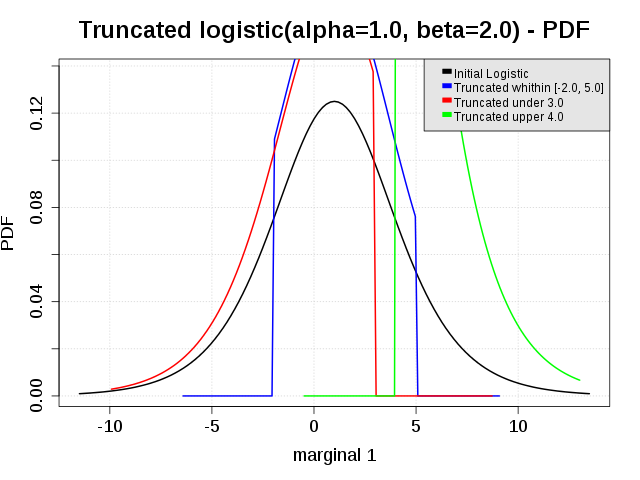
\includegraphics[width=10cm]{Figures/truncatedDistribution_pdf.png}
  \end{center}
  \caption{PDF of several truncated Logistic distributions}
  \label{truncatedDistribution_pdf}
\end{figure}

\begin{figure}[H]
  \begin{center}
    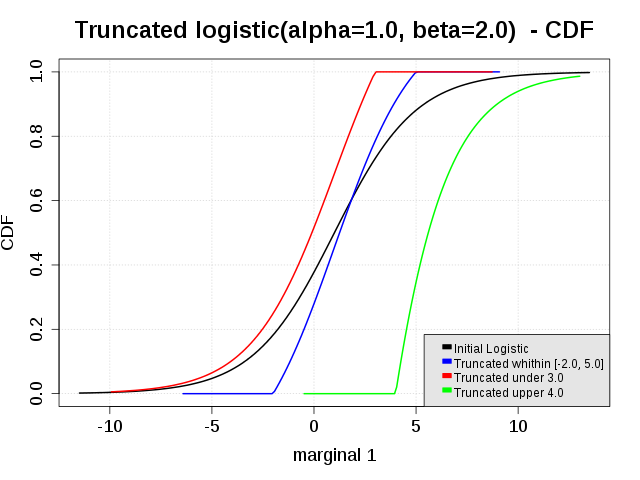
\includegraphics[width=10cm]{Figures/truncatedDistribution_cdf.png}
  \end{center}
  \caption{CDF of several truncated Logistic distributions}
  \label{truncatedDistribution_cdf}
\end{figure}

\newpage % Copyright 2005-2016 Airbus-EDF-IMACS-Phimeca
% Permission is granted to copy, distribute and/or modify this document
% under the terms of the GNU Free Documentation License, Version 1.2
% or any later version published by the Free Software Foundation;
% with no Invariant Sections, no Front-Cover Texts, and no Back-Cover
% Texts.  A copy of the license is included in the section entitled "GNU
% Free Documentation License".
\renewcommand{\filename}{docUC_InputNoData_Copula}
\renewcommand{\filetitle}{UC : List of Copula}

% \HeaderNNIILevel
% \HeaderIILevel
\HeaderIIILevel








The objective of this Use Case is to manipulate copulas of OpenTURNS.\\

A copula may be considered as the restriction to $[0,1]^n$ of a distribution with uniform 1D marginals on $[0,1]$ and this copula as copula. That's why an object of type {\itshape Copula} offers the same methods as an object of type {\itshape Distribution} (see U.C. \ref{manipulation_distribution} to have the list of the methods).\\

Details on copula may be found in the Reference Guide (\extref{ReferenceGuide}{see file Reference Guide - Step B -- Copula}{stepB}).\\



\index{Copula!Ali-Mikhail-Haq}
\index{Copula!Clayton}
\index{Copula!Composed copula}
\index{Copula!Farlie-Gumbel-Morgenstern}
\index{Copula!Frank}
\index{Copula!Gumbel}
\index{Copula!Independent}
\index{Copula!Normal}
\index{Copula!Min}
\index{Copula!Mixture}
\index{Copula!Sklar}
\index{Correlation!Correlation matrix of the Normal copula}
\index{Correlation!Spearman rank correlation matrix}


OpenTURNS proposes the copulas listed in Table.\ref{ListCopulas}.  Table.\ref{CaracCopulas} gives the main copula features, where AMH means Ali-Mikhail-Haq and FGM means Farlie-Gumbel-Morgenstern.

\begin{table}[H]
  \begin{center}
    \begin{tabular}{|l|c|c|c|c|}
      \hline
      Copula & Archimedean & Independent & Elliptical & Other \\
      \hline
      AMH & $\times$ & for $\theta = 0$ &  & \\
      \hline
      Clayton & $\times$ &  for $\theta = 0$ & &\\
      \hline
      ComposedCopula & & \parbox[c]{4cm}{if each copula is Independent} & \parbox[c]{4cm}{if each copula is Normal} & $\times$ \\
      \hline
      FGM & & for $\theta = 0$ & & $\times$ \\
      \hline
      Frank & $\times$ & for $\theta = 0$ & &\\
      \hline
      Gumbel & $\times$ & for $\theta = 1 $ & &\\
      \hline
      Independant &$\times$ & $\times$& $\times$&\\
      \hline
      Min & & & &$\times$\\
      \hline
      Normal & & for $\mat{R} = \mat{I}$ & $\times$ &\\
      \hline
      SklarCopula & \parbox[c]{4cm}{if coming from a distribution with Archimedean copula}& the same & the same & $\times$ \\
      \hline
    \end{tabular}
    \caption{Features of the OpenTURNS copula.}
    \label{CaracCopulas}
  \end{center}
\end{table}
\textspace\\





\newcommand\B{\rule[-2.4ex]{0pt}{0pt}}
\newcommand\Top{\rule{0pt}{4.8ex}}

\begin{table}[H]
  \begin{center}
    \begin{tabular}{|l|c|c|c|}
      \hline
      Name & Dimension & $C(u_1, \cdots, u_n)$ & Parameters\textspace\Top\B\\
      \hline
      AMH & 2 & $\displaystyle \frac{u_1u_2}{1-\theta(1-u_1)(1-u_2)}$ & $|\theta|<1$\textspace\Top\B\\
      \hline
      Clayton & 2 & $\displaystyle \left(u_1^{-\theta}+u_2^{-\theta}-1\right)^{-1/\theta}$ & $\theta \geq 0$\textspace\Top\B\\
      \hline
      FGM & $2$ & $\displaystyle u_1u_2 (1 + \theta(1 - u_1)(1 - u_2))$ & $\theta\in[-1,1]$\textspace\Top\B\\
      \hline
      Frank & 2 & $\left\{^{\strut}\begin{array}{ll}\displaystyle -\frac{1}{\theta}\log\left(1+\frac{(e^{-\theta u_1}-1)(e^{-\theta u_2}-1}{e^{-\theta}-1}\right) & \mbox{ for }\theta\neq 0\\
        \displaystyle  u_1u_2&\mbox{ for }\theta=0
      \end{array}\right._{\strut}$ & $\theta>0$\textspace\Top\B\\
      \hline
      Gumbel & 2 & $\displaystyle \exp\left(-\left((-\log(u_1))^{\theta}+(-\log(u_2))^{\theta}\right)^{1/\theta}\right)$ & $\theta \geq 1$\textspace\Top\B\\
      \hline
      Independent & $n$ & $\displaystyle \prod_{i=1}^{n} u_i$ & $n$ \textspace\Top\B\\
      \hline
      Min & $n$ & $\displaystyle \min(u_1,\dots,u_n)$ & $n$\textspace\Top\B\\
      \hline
      Normal & 2 &  $\displaystyle\int_{-\infty}^{\Phi^{-1}(u_1)}\int_{-\infty}^{\Phi^{-1}(u_2)}\frac{1}{2\pi\sqrt{1-\rho^2}}\exp\left(-\frac{s^2-2\rho st+t^2}{2(1-\rho^2)}\right)\,\Diff s\,\Diff t$ \mathspace\Top\B & $\begin{array}{l}
        \mat{R} = \left(\begin{array}{cc}
          1 & \rho \\
          \rho & 1
        \end{array}
        \right)^{\strut}\\
        \rho \in (-1,1)
      \end{array}$\\
      \hline
      Normal & $n$ & $\displaystyle\int_{-\infty}^{\Phi^{-1}(u_1)}\cdots \int_{-\infty}^{\Phi^{-1}(u_n)}\frac{1}{(2\pi)^{n/2} \sqrt{\det(\mat{R})}}\exp\left(-\frac{1}{2}\vect{x}^t \mat{R}^{-1} \vect{x} \right)\,\Diff \vect{x}$ & $\mat{R}$, SPD \textspace\Top\B\\
      \hline
      Sklar & $n$ & $\displaystyle F\left(F_1^{-1}(u_1), \dots, F_n^{-1}(u_n)\right)$ & $-$\textspace\Top\B\\
      \hline
    \end{tabular}
    \caption{Expressions of the copulas of OpenTURNS.}
    \label{ListCopulas}
  \end{center}
\end{table}
\textspace\\


Furthermore, OpenTURNS allows to extract the copula $C$ from any $n$ dimensional distribution, thanks to the inverse of the Sklar theorem :
\begin{align*}
  C(u_1, \dots, u_n) = F(F_1^{-1}(u_1), \dots, F_n^{-1}(u_n))
\end{align*}
where $F$ is the cumulative density function of the distribution and $F_i$ its respective marginals. This copula is denoted \emph{Sklar Copula} within OpenTURNS.\\

OpenTURNS also allows to create some copula as the product of other copulas : if $C_1$ and $C_2$ are two copulas respectively of random vectors in  $\Rset^{n_1}$ and $\Rset^{n_2}$, we can create the copula of a random vector of $\Rset^{n_1+n_2}$, noted $C$ as follows :
\begin{align*}
  C(u_1, \cdots, u_n) = C_1(u_1, \cdots, u_{n_1}) C_2(u_{n_1+1}, \cdots, u_{n_1+n_2})
\end{align*}
It means that both subvectors $(u_1, \cdots, u_{n_1})$ and $(u_{n_1+1}, \cdots, u_{n_1+n_2})$ of $\Rset^{n_1}$ and $\Rset^{n_2}$ are independent.\\

OpenTURNS also creates some mixtures of copulas (the density is a linear combination of some copulas densities) thanks to the object {\itshape Mixture} (see the use case \label{Mixture}). Note that the result still remains a copula.\\

OpenTURNS also builds ordinal sums of copulas from a collection of $n$ copulas $(C_1, \dots, C_n)$, each one being of the same dimension $d$ and a collection of bounds $(\alpha_1, \dots, \alpha_{n+1})$ in $]0,1[$. The ordinal sums of copulas is defined by:
\begin{equation}
 C(\vect{u}) = \left\{
    \begin{array}{ll}
       \alpha_i+C_i \left( \dfrac{u_1-\alpha_i}{\alpha_{i+1} - \alpha_i} \right) & \mbox{ if } \vect{u} \in [\alpha_i, \alpha_{i+1}[ \\
       M_d(\vect{u}) & \mbox{ else } 
    \end{array}
    \right.
\end{equation}
with $M_d$ the Min-copula: $M_d(\vect{u}) = \min_{k=1 \dots d} u_k$ and where, for convenience, we noted $\alpha_0=0$ and $\alpha_n=1$.\\
Note that if  $\alpha_i=\alpha_{i+1}$ then the copula $C_{i+1}$ is erased from the list, for $i=0 \dots n-1$.




 
\noindent%
\requirements{
  \begin{description}
  \item[$\bullet$] none
  \end{description}
}
             {
               \begin{description}
               \item[$\bullet$] all the copula named according to the rule : {\itshape typeCopula}
               \item[type:] usual copula (for example NormalCopula,...)
               \item[$\bullet$] a composed copula : {\itshape finalCopula}
               \item[type:] ComposedCopula
               \end{description}
             }

             \textspace\\
             Python script for this UseCase :

             \inputscript{script_docUC_InputNoData_Copula}

             \textspace\\

             Refer to the Reference Guide to get the graphs of the pdf iso-curves of each copula.

\newpage % Copyright 2005-2016 Airbus-EDF-IMACS-Phimeca
% Permission is granted to copy, distribute and/or modify this document
% under the terms of the GNU Free Documentation License, Version 1.2
% or any later version published by the Free Software Foundation;
% with no Invariant Sections, no Front-Cover Texts, and no Back-Cover
% Texts.  A copy of the license is included in the section entitled "GNU
% Free Documentation License".
\renewcommand{\filename}{docUC_InputNoData_ComposedDistribution.tex}
\renewcommand{\filetitle}{UC : Creation  of nD distribution from (marginals, copula)}

% \HeaderNNIILevel
% \HeaderIILevel
\HeaderIIILevel





\index{Composed Distribution}
\index{Copula!Independent}
\index{Copula!Normal}
\index{Correlation!Correlation matrix of the Normal copula}
\index{Correlation!Spearman rank correlation matrix}
\index{Distribution!Marginals and copula}


The objective of the Use Case is to model a distribution, described by its marginal distributions and its dependence structure (a particular copula). A simplified way is proposed when the copula is the independent one.\\

Details on copula may be found in the Reference Guide (\extref{ReferenceGuide}{see file Reference Guide - Step B -- Copula}{stepB}).\\

This Use Case is particularly adapted to the modelisation of the distribution of the input random vector.\\

The example here is a distribution of dimension 3 defined by :
\begin{itemize}
\item Beta, Triangular and Uniform marginals,
\item an independent copula.
\end{itemize}

\noindent%
\requirements{
  \begin{description}
  \item[$\bullet$] none
  \end{description}
}
             {
               \begin{description}
               \item[$\bullet$] a nD distribution : {\itshape myDistribution}
               \item[type:] Distribution which implementation is a ComposedDistribution
               \end{description}
             }

             \textspace\\
             Python script for this UseCase :

             \inputscript{script_docUC_InputNoData_ComposedDistribution}

\newpage % Copyright (C) 2005-2015 Airbus - EDF - IMACS - Phimeca
% Permission is granted to copy, distribute and/or modify this document
% under the terms of the GNU Free Documentation License, Version 1.2
% or any later version published by the Free Software Foundation;
% with no Invariant Sections, no Front-Cover Texts, and no Back-Cover
% Texts.  A copy of the license is included in the section entitled "GNU
% Free Documentation License".
\renewcommand{\filename}{docUC_InputNoData_Mixture.tex}
\renewcommand{\filetitle}{UC : Creation  of a nD distribution from a Mixture}

% \HeaderNNIILevel
% \HeaderIILevel
\HeaderIIILevel

\label{Mixture}

\index{Distribution!Mixture}
\index{Graph!PDF-CDF curves}
\index{Graph Manipulation!Bounding box}
\index{Graph Manipulation!View}
\index{Graph Manipulation!Show}

In OpenTURNS, a Mixture is a distribution which probability density function is a linear combination of probability density functions.\\

The objective of this Use Case is to model a distribution, defined as a mixture :
\begin {equation}\label{mixPDF}
  p(\vect{x}) = \sum_{i=1}^{n} a_i p_i(\vect{x})
\end{equation}
where
\begin {equation}\label{mixcons}
  \sum_{i=1}^{n} a_i = 1
\end{equation}
and
\begin {equation}\label{mixcons2}
  \forall i,  \, a_i \geq 0
\end{equation}

OpenTURNS automatically normalizes the  weights so the User can give $a_i$ which don't verify the constraint (\ref{mixcons}). \\
By default, the weights are taken equal to $\frac{1}{n}$.\\

The example here is a mixture of three univariate distributions: Triangular(1.0, 2.0, 4.0), Normal(-1.0, 1.0) and Uniform(5.0, 6.0), with respective weights : (0.2, 0.3, 0.5).\\
The PDF and CDF graphs the mixture distribution are drawn in Figures \ref{mixtureGraphPDF} and  \ref{mixtureGraphCDF}.\\

Note that it is possible to create a mixture of copula. The result still remains a copula.

\textspace\\
\noindent%
\requirements{
  \begin{description}
  \item[$\bullet$] some distributions : {\itshape dist1, dist2}
  \item[type:] Distribution
  \item[$\bullet$] some  copulas: {\itshape cop1, cop2}
  \item[type:] Distribution
  \end{description}
}
             {
               \begin{description}
               \item[$\bullet$] a mixture distribution : {\itshape myMixtDist}
               \item[type:] Mixture
               \item[$\bullet$] a mixture copula : {\itshape myMixtCop}
               \item[type:] Mixture
               \end{description}
             }

             \textspace\\
             Python script for this UseCase :

             \inputscript{script_docUC_InputNoData_Mixture}

             \textspace\\


             \begin{figure}[H]
               \begin{center}
                 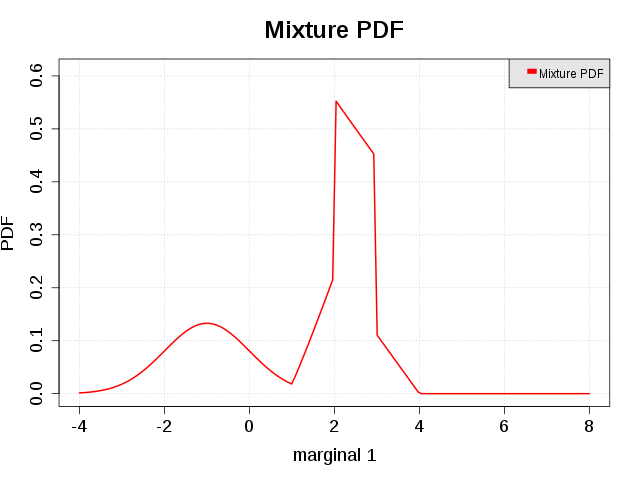
\includegraphics[width=10cm]{Figures/pdf_Mixture.png}
                 \caption{PDF of the Mixture distribution = 0.2*Triangular(1.0, 2.0, 4.0) + 0.5*Normal(-1.0, 1.0) + 0.3*Uniform(5.0, 6.0)}
                 \label{mixtureGraphPDF}
               \end{center}
             \end{figure}

             \begin{figure}[H]
               \begin{center}
                 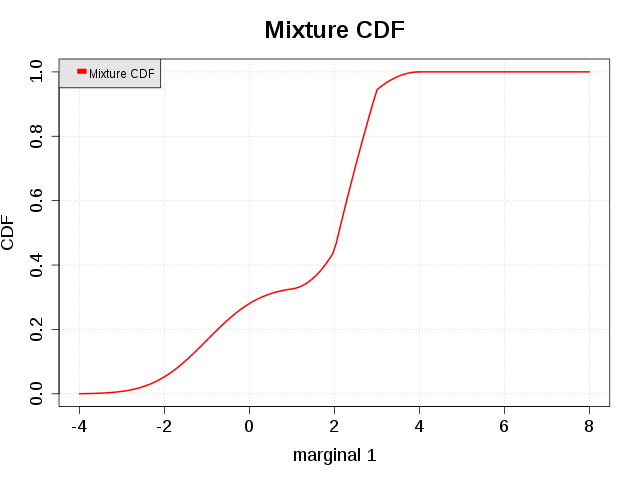
\includegraphics[width=10cm]{Figures/cdf_Mixture.png}
                 \caption{CDF of the Mixture distribution = 0.2*Triangular(1.0, 2.0, 4.0) + 0.5*Normal(-1.0, 1.0) + 0.3*Uniform(5.0, 6.0)}
                 \label{mixtureGraphCDF}
               \end{center}
             \end{figure}

%\newpage % Copyright (C) 2005-2015 Airbus - EDF - IMACS - Phimeca
% Permission is granted to copy, distribute and/or modify this document
% under the terms of the GNU Free Documentation License, Version 1.2
% or any later version published by the Free Software Foundation;
% with no Invariant Sections, no Front-Cover Texts, and no Back-Cover
% Texts.  A copy of the license is included in the section entitled "GNU
% Free Documentation License".
\renewcommand{\filename}{docUC_InputNoData_ProductDistribution.tex}
\renewcommand{\filetitle}{UC : Creation  of 1D distribution as the product of 1D distributions}

% \HeaderNNIILevel
% \HeaderIILevel
\HeaderIIILevel

\index{Product Distribution}

The objective of the Use Case is to create a distribution, defined as the prodcut of univariate distributions.\\

If we note $\mathcal{L}_X$ and $\mathcal{L}_Y$ two univariate distributions, OpenTURNS enables to easily create the distribution  $\mathcal{L}$ of the random variable $Z$ defined by:
\begin{align}
  Z=XY
\end{align}
where $(X,Y)$ are independent with respective marginal distributions  $\mathcal{L}_X$ and $\mathcal{L}_Y$.

\textspace\\

\noindent%
\requirements{
  \begin{description}
  \item[$\bullet$] two independent  univariate distribution : {\itshape distX, distY}
  \item[type:] Distribution
  \end{description}
}
{
  \begin{description}
  \item[$\bullet$] the product distribution : {\itshape distZ}
  \item[type:] ProductDistribution
  \end{description}
}

\textspace\\
Python script for this UseCase :

\inputscript{script_docUC_InputNoData_ProductDistribution}

\textspace\\

The figure \ref{prodDist} illustrates the product distribution where:
\begin{itemize}
\item  $\mathcal{L}_X = Uniform(0, 1)$,
\item  $\mathcal{L}_Y = Uniform(2, 3)$.
\end{itemize}




\begin{figure}[H]
  \begin{center}
    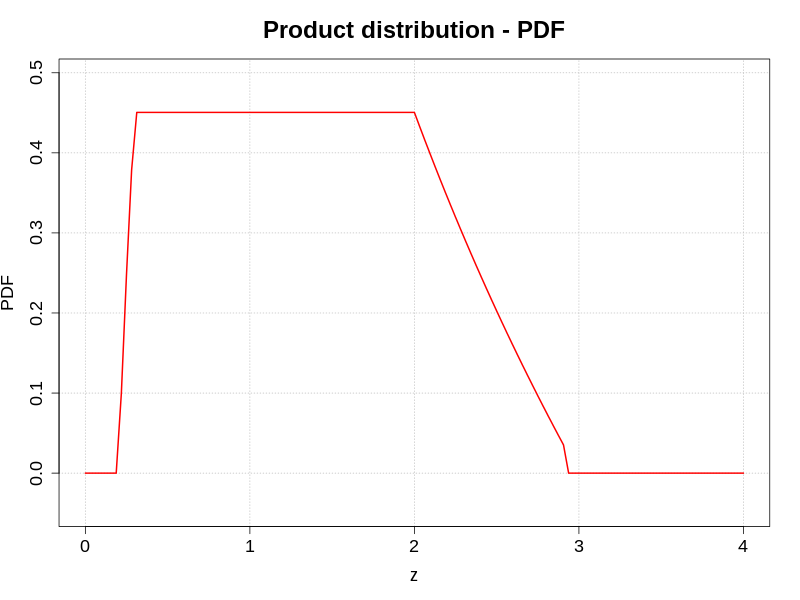
\includegraphics[width=7cm]{Figures/productDist.png}
    \caption{PDF $Z=XY$ where $(X, Y)$ are independent with respective marginal distributions $Uniform(0, 1$) and $Uniform(2, 3)$.}
    \label{prodDist}
  \end{center}
\end{figure}

\newpage % Copyright (C) 2005-2015 Airbus - EDF - IMACS - Phimeca
% Permission is granted to copy, distribute and/or modify this document
% under the terms of the GNU Free Documentation License, Version 1.2
% or any later version published by the Free Software Foundation;
% with no Invariant Sections, no Front-Cover Texts, and no Back-Cover
% Texts.  A copy of the license is included in the section entitled "GNU
% Free Documentation License".
\renewcommand{\filename}{docUC_InputNoData_CompositeDistribution.tex}
\renewcommand{\filetitle}{UC : Creation  of 1D distribution from a 1D distribution}

% \HeaderNNIILevel
% \HeaderIILevel
\HeaderIIILevel





\index{Composed Distribution}


The objective of the Use Case is to create a distribution, defined as the push-forward distribution of a scalar distribution  by a transformation $\Rset \rightarrow \Rset$. \\

If we note $\mathcal{L}_0$ a scalar distribution, $f: \Rset \rightarrow \Rset$ a mapping, then OpenTURNS enables to easily create the push-forward distribution $\mathcal{L}$ defined by: 
\begin{align}
\mathcal{L} = f(\mathcal{L}_0)
\end{align}
which means that for all scalar random variable $X$ following the distribution $\mathcal{L}_0$, $Y=f(X)$ follows the distribution $\mathcal{L}$. \\

Note that for the following usual transformations $f$, a simplified notation has been implemented: \emph{cos, sin, tan, acos, asin, atan, cosh, sinh, tanh, acosh, asinh, atanh, exp,  log, ln, pow, inverse, sqr, sqrt, cbrt, abs}.  If the operators are chained, they are applied from left to right. See the foolowing script for some examples.


             \textspace\\

\noindent%
\requirements{
  \begin{description}
  \item[$\bullet$] a scalar distribution : {\itshape myAntecedentDist}
  \item[type:] Distribution
  \end{description}

  \begin{description}
  \item[$\bullet$] a mapping  $\Rset \rightarrow \Rset$: {\itshape f}
  \item[type:] NumericalMathFunction
  \end{description}
}
             {
  \begin{description}
  \item[$\bullet$] a scalar distribution : {\itshape myImageDist}
  \item[type:] CompositeDistribution
  \end{description}
             }

             \textspace\\
             Python script for this UseCase :

             \inputscript{script_docUC_InputNoData_CompositeDistribution}

             \textspace\\
The following figures illustrate the cases where $\mathcal{L}_0$ is the Normal() distribution and $f$ the function defined by:
\begin{itemize}
  \item  $f(x)=\sin(x) + \cos(x)$ in the figure  \ref{Imagedist};
  \item  $f(x)=\exp(x)$  in the figure   \ref{Imagedist2};
  \item  $f(x)=\sqrt{|x|}$  in the figure   \ref{Imagedist3}.
\end{itemize}




\begin{figure}[H]
  \begin{minipage}{9cm}
    \begin{center}
      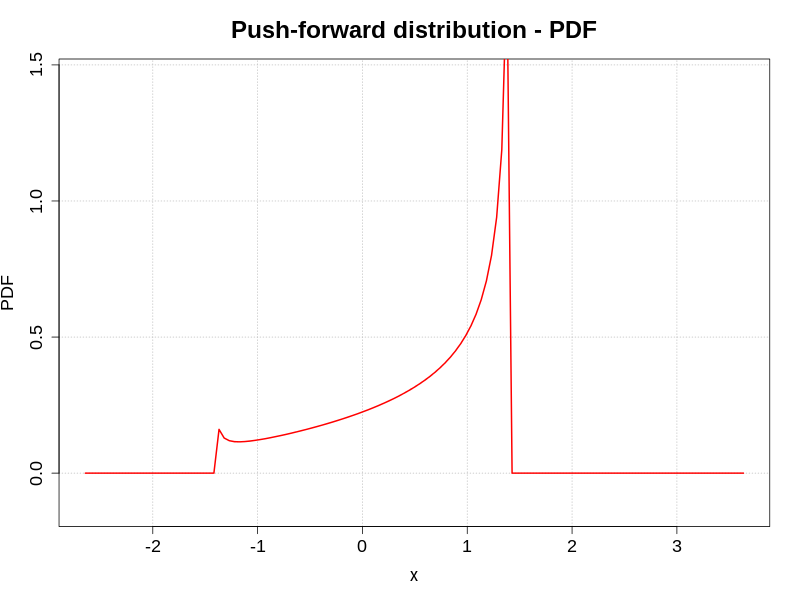
\includegraphics[width=7cm]{Figures/ImageDist.png}
      \caption{PDF of the push-forward distribution of a Normal() mapped through $f(x)=\sin(x) + \cos(x)$}
      \label{Imagedist}
    \end{center}
  \end{minipage}
  \hfill
  \begin{minipage}{9cm}
    \begin{center}
      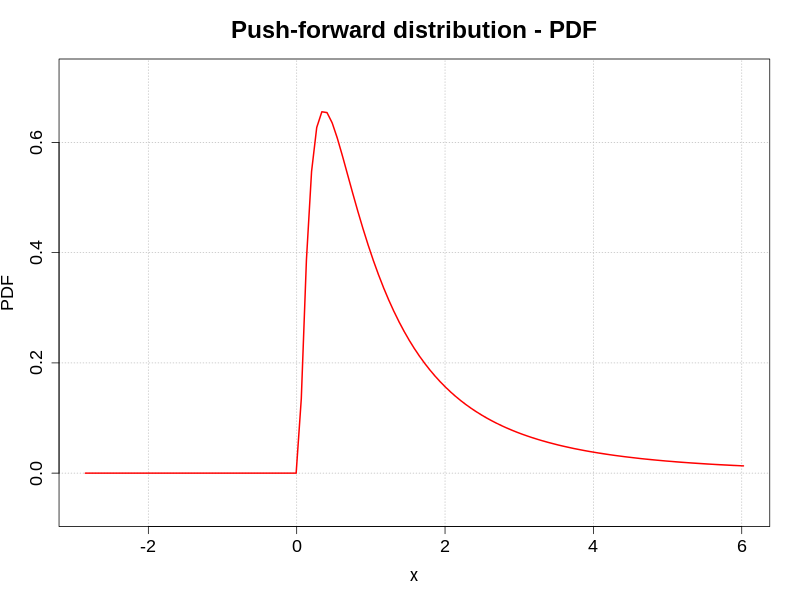
\includegraphics[width=7cm]{Figures/ImageDist2.png}
      \caption{PDF of the push-forward distribution of a Normal() mapped through $f(x)=\exp(x)$}
      \label{Imagedist2}
    \end{center}
  \end{minipage}
\end{figure}

\begin{figure}[H]
  \begin{center}
      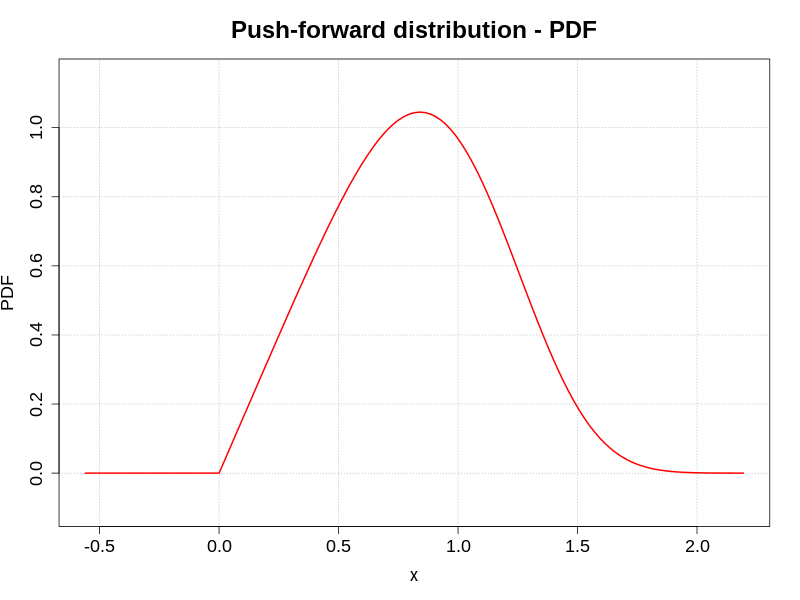
\includegraphics[width=7cm]{Figures/ImageDist3.png}
      \caption{PDF of the push-forward distribution of a Normal() mapped through $f(x)=\sqrt{|x|}$}
      \label{Imagedist3}
    \end{center}
\end{figure}

\newpage % Copyright 2005-2016 Airbus-EDF-IMACS-Phimeca
% Permission is granted to copy, distribute and/or modify this document
% under the terms of the GNU Free Documentation License, Version 1.2
% or any later version published by the Free Software Foundation;
% with no Invariant Sections, no Front-Cover Texts, and no Back-Cover
% Texts.  A copy of the license is included in the section entitled "GNU
% Free Documentation License".
\renewcommand{\filename}{docUC_InputNoData_DistManipulation.tex}
\renewcommand{\filetitle}{UC : Manipulation of a distribution}

% \HeaderNNIILevel
% \HeaderIILevel
\HeaderIIILevel


\label{manipulation_distribution}


\index{Copula!Estimation from sample}
\index{Mixture}
\index{Graph!Specifying the file format}
\index{Graph!PDF-CDF curves}
\index{Graph!PDF-CDF isocurves}
\index{Graph Manipulation!Bounding box}
\index{Graph Manipulation!View}
\index{Graph Manipulation!Show}
\index{Quantile!Distribution evaluation}
\index{Sample Statistics!Sample Generation}



The objective of this Use Case is to describe the main functionalities that OpenTURNS enables to manipulate a distribution of dimension $n \geq 1$.\\



Let's note $\vect{X} = (X_1, \cdots, X_n)$ the random vector associated to that distribution, which PDF is note $p$. OpenTURNS enables :
\begin{itemize}
\item to ask for the dimension, with the method {\itshape getDimension};
\item if $n >1$, to extract the extracted distribution of dimension $k<n$ corresponding to $k$ 1D marginals, with the method {\itshape getMarginal};
\item to get the copula, with the method {\itshape getCopula}: if the distribution is of type ComposedDistribution, the copula is the one specified at the creation of the ComposedDistribution. If the distribution is not that sort (for example, a KernelMixture, a Mixture, a RandomMixture), the copula is computed from the Sklar theorem;
\item to ask for some properties on the copula, with the method {\itshape hasIndependentCopula, hasEllipticalCopula}, only for the types Usual Distribution and ComposedDistribution (defined from the 1D marginals and a copula);
\item to evaluate the mean vector (potentially of dimension 1), the covariance matrix (potentially of dimension $1\times 1$), the standard deviation, skewness and kurtosis vectors (potentially of dimension 1), with the methods {\itshape getMean, getStandardDeviation, getCovariance, getKurtosis, getSkewness}, defined by the following expressions :
  \begin{align*}
    \left\{
      \begin{array}{lcl}
        \displaystyle \vect{E}[\vect{X}] & = & \displaystyle (E[X_1], \cdots, E[X_n]) \\
        \displaystyle \mat{StdDev}[\vect{X}] & = & \displaystyle (\sqrt{E[(X_1-E[X_1])^2]}, \cdots, \sqrt{E[(X_n-E[X_n])^2]}) \\
        \displaystyle \mat{Cov}[\vect{X}] & = & \displaystyle (E\left[(X_i-E[X_i])(X_j-E[X_j])\right])_{i,j} \\
        \displaystyle \vect{skewness}[\vect{X}] & = & \displaystyle (E\left[\left(\frac{(X_1-E[X_1])}{\sqrt{\Var{X_1}}}\right)^3\right], \cdots, E\left[\left(\frac{(X_n-E[X_n])}{\sqrt{\Var{X_n}}}\right)^3\right]) \\
        \displaystyle \vect{kurtosis}[\vect{X}] & = & \displaystyle (E\left[\left(\frac{(X_1-E[X_1])}{\sqrt{\Var{X_1}}}\right)^4\right], \cdots, E\left[\left(\frac{(X_n-E[X_n])}{\sqrt{\Var{X_n}}}\right)^4\right])
      \end{array}
    \right.
  \end{align*}
\item to evaluate the roughness, with the method {\itshape getRoughness}, defined by :
  \begin{align*}
    roughness(\vect{X}) = ||p||_{\cL^2} = \sqrt{\int_\vect{x} p^2(\vect{x})d\vect{x}}
  \end{align*}

\item to get one realization or simultaneously $n$ realizations, with the method {\itshape getRealization, getSample},
\item to evaluate the Cumulative Distribution Function (CDF), the complementary CDF, the Probability Density Function (PDF) on a scalar (1D distribution only), on a point or on a numerical sample with the method {\itshape computeCDF, computePDF},
\item to evaluate the probability content of a given interval, with the method {\itshape computeProbability},
\item to evaluate a quantile (or a group of quantiles) or a complementary quantile, (or a group of complementary quantile) with the method {\itshape computeQuantile}. If the distribution if of dimension $n>1$, the $p-$ quantile is the hyper surface in $\Rset^n$ defined by  $\{\vect{x}\in \Rset^n, F(x_1, \dots, x_n) = p \}$ where $F$ is the CDF. OpenTURNS makes the choice to return one particular point among these points : $(x_1^p, \dots, x_n^p)$ such that $\forall i, F_i(x_i^p) =  \tau$ where $F_i$ is the marginal of component $X_i$ and $F(x_1, \dots, x_n) = C(\tau, \dots, \tau)$ where $C$ is the distribution copula. Thus, OpenTURNS resolves the equation $ C(\tau, \dots, \tau)=p$ then computes $F_i^{-1}(\tau) = x_i^p$.\\
  Note that the point  $(x_1^p, \dots, x_n^p)$ belongs to the curve $(F_1^{-1}(s), \dots, F_n^{-1}(s))$. In dimension 2, OpenTURNS draws the curve $s \mapsto (F_1^{-1}(s), F_2^{-1}(s))$ and points the quantile of order $p$, with $p\in [p_{min}, p_{max}]$ discretized with $N$ points: see the method {\itshape drawQuantiles}.
\item to evaluate the derivative of the CDF or PDF with respect to the parameters of the distribution at a particular point, with the methods {\itshape computeCDFGradient, computePDFGradient},
\item to evaluate the characteristic function of the distribution, only for the following distributions : Chi2, Gamma, Laplace, Logistic, univariate Normal, Rayleigh, Triangular, univariate TruncatedNormal, Uniform, KernelMixture (which includes a KernelSmoothing without bound treatment), Mixture, RandomMixture;
\item to draw :
  \begin{itemize}
  \item for a 1D distribution : the PDF and CDF curves, with the methods {\itshape drawPDF, drawCDF},
  \item for a 2D distribution : the PDF and CDF iso-curves, with the methods {\itshape drawPDF, drawCDF}, and the PDF and CDF curves of its 1D marginals, with the methods {\itshape drawMarginal1DPDF, drawMarginal1DCDF} ,
  \item for a $nD$ with $n\geq 3$ distribution : the PDF and CDF of each 1D marginal, with the methods {\itshape drawMarginal1DPDF, drawMarginal1DCDF} and the PDF and CDF iso-curves for a specified 2D marginal, with the methods {\itshape drawMarginal2DPDF, drawMarginal2DCDF}.
  \end{itemize}
\end{itemize}

Let's note that it is possible to visualize a graph whithin the TUI without creating the associated files, thanks to the command {\itshape Show}.\\

\noindent%
\requirements{
  \begin{description}
  \item[$\bullet$] three distributions of dimension 1, 2 and 3 : {\itshape dist\_1, dist\_2, dist\_3}
  \item[type:] Distribution
  \end{description}
}
{
  \begin{description}
  \item[$\bullet$] graphes, numerical points, ...
  \end{description}
}

\textspace\\
Python script for this UseCase :

\inputscript{script_docUC_InputNoData_DistManipulation}

\textspace\\


We draw respectively  in Figures \ref{tulipe} and \ref{contour2D_example2} the iso-curves of the PDF of the two following  distributions :
\begin{itemize}
\item Distribution 1 : Mixture of Normal distributions of dimension 2
\item Distribution 2 : Composed Distribution, with a Gumbel copula and each marginal some mixture of normals of dimension 1.
\end{itemize}



\begin{figure}[H]
  \begin{center}
    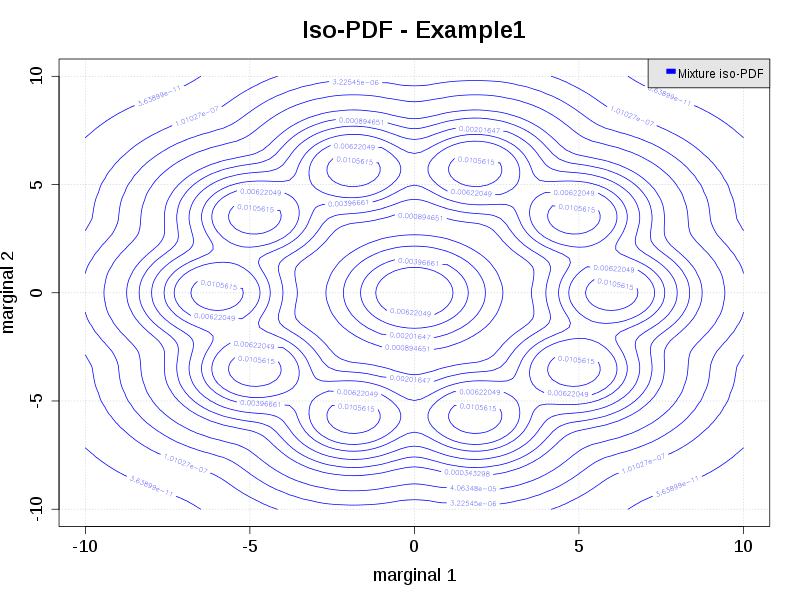
\includegraphics[width=10cm]{Figures/contour2D_tulipe.png}
  \end{center}
  \caption{Iso-curves of the PDF of Distribution 1 : Mixture of Normal distributions of dimension 2.}
  \label{tulipe}
\end{figure}

\begin{figure}[H]
  \begin{center}
    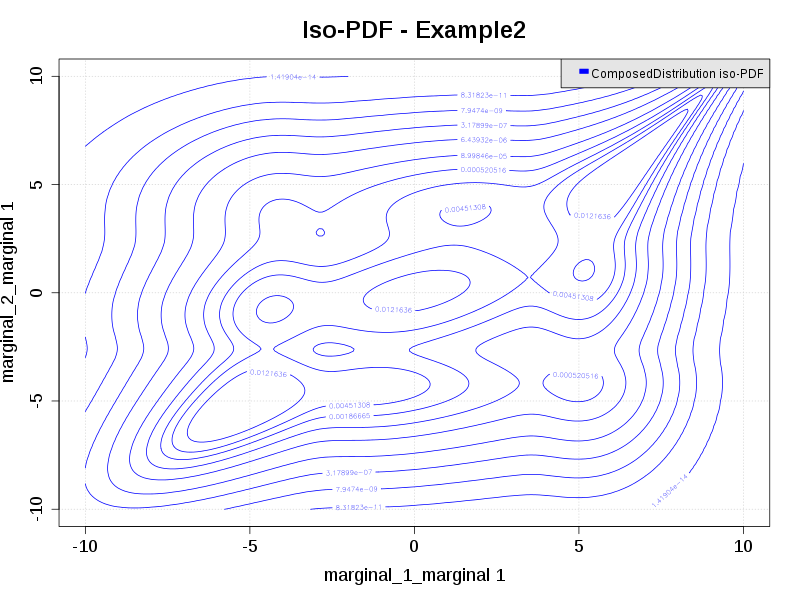
\includegraphics[width=10cm]{Figures/contour2D_2.png}
  \end{center}
  \caption{Iso-curves of the PDF of Distribution 2 : Composed Distribution, with a Gumbel copula and each marginal some mixture of normals of dimension 1.}
  \label{contour2D_example2}
\end{figure}

In the Figure \ref{quantileCurve}, we draw the quantile curve $p \mapsto F_1^{-1}(p)$ where  $p\in[0.1, 0.9]$ of the univariate $\cN(0,1)$ distribution.\\

In the Figure \ref{quantileCurve2d}, we draw the curve  $s \mapsto (F_1^{-1}(s), F_2^{-1}(s))$  and we point the quantiles of order $p \in [0.1, 0.9]$ regularly discretized into 101 points, of the bivariate distribution defined by: the margins are respectively  $\cN(0,1)$ and Triangular(0.0, 2.0, 3.0) and the copula is the Clayton copula($\theta=2.3$).


\begin{figure}[H]
  \begin{minipage}{9cm}
    \begin{center}
      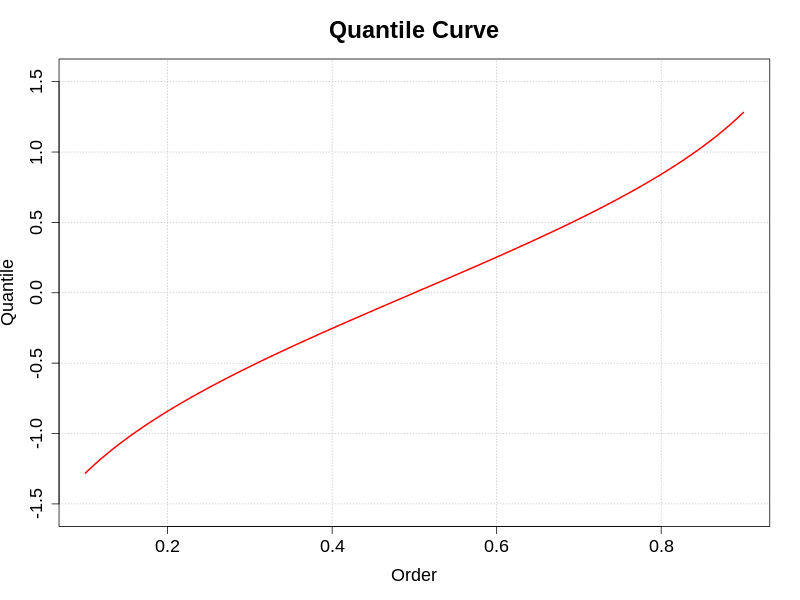
\includegraphics[width=7cm]{Figures/QuantileCurve2.png}
      \caption{A quantile curve in dimension 1.}
      \label{quantileCurve}
    \end{center}
  \end{minipage}
  \hfill
  \begin{minipage}{9cm}
    \begin{center}
      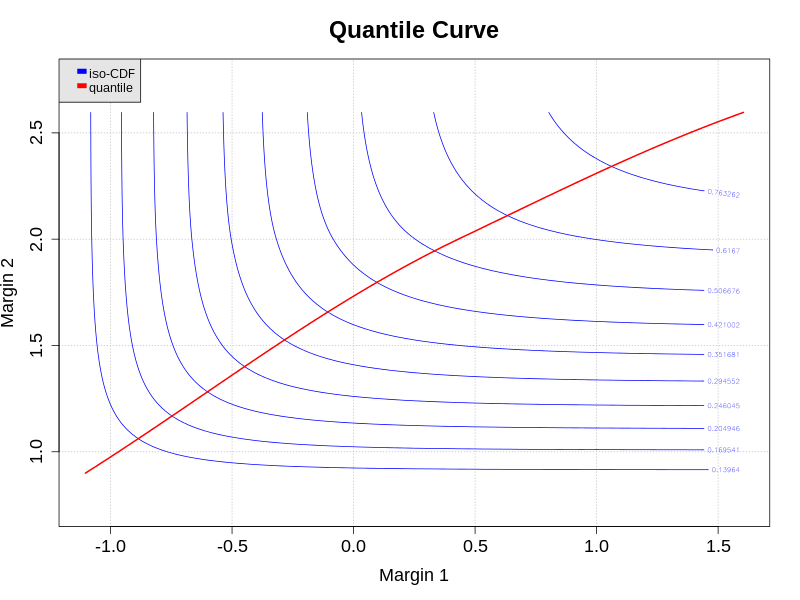
\includegraphics[width=7cm]{Figures/QuantileCurve.png}
      \caption{A quantile curve in dimension 2.}
      \label{quantileCurve2d}
    \end{center}
  \end{minipage}
\end{figure}

\newpage % Copyright (C) 2005-2015 Airbus - EDF - IMACS - Phimeca
% Permission is granted to copy, distribute and/or modify this document
% under the terms of the GNU Free Documentation License, Version 1.2
% or any later version published by the Free Software Foundation;
% with no Invariant Sections, no Front-Cover Texts, and no Back-Cover
% Texts.  A copy of the license is included in the section entitled "GNU
% Free Documentation License".
\renewcommand{\filename}{docUC_InputNoData_CustomDistFromPython.tex}
\renewcommand{\filetitle}{UC : Creation of a custom distribution or copula from the python script}

% \HeaderNNIILevelx
% \HeaderIILevel
\HeaderIIILevel


\label{creation_distribution}

The objective of this Use Case is to describe how to create one own distribution or copula from a python script.\\


The principle is to inherit from the \textit{PythonDistribution} class and overload the methods of the Distribution object.\\
To create a Copula, one has to implement \emph{return = True} in the method {\itshape isCopula()}. Care: it is under the User's responsability.\\

Then an instance of the new class can be passed on into a Distribution object.\\
At least computeCDF should be overriden.

\requirements{
  \begin{description}
  \item[$\bullet$] at least a CDF function expressed in python.
  \end{description}
}
{
  \begin{description}
  \item[$\bullet$] an object proposing the same services as Distribution does.
  \item[type:] Distribution
  \end{description}
}

\textspace\\
Python script for this UseCase :

\inputscript{script_docUC_InputNoData_CustomDistFromPython}

\newpage % Copyright (C) 2005-2015 Airbus - EDF - IMACS - Phimeca
% Permission is granted to copy, distribute and/or modify this document
% under the terms of the GNU Free Documentation License, Version 1.2
% or any later version published by the Free Software Foundation;
% with no Invariant Sections, no Front-Cover Texts, and no Back-Cover
% Texts.  A copy of the license is included in the section entitled "GNU
% Free Documentation License".
\renewcommand{\filename}{docUC_InputNoData_CustomRandVectFromPython.tex}
\renewcommand{\filetitle}{UC : Creation of a custom random vector from the python script}

% \HeaderNNIILevel
% \HeaderIILevel
\HeaderIIILevel


\label{manipulation_random vector}

The objective of this Use Case is to describe the main functionalities enabling to define a random vector from the python script.\\



Details on each object may be found in the User Manual  (\extref{UserManual_TUI}{see User Manual - Probabilistic modeling}{probModeling}).\\

The principle is to inherit from the \textit{PythonRandomVector} class and overload the methods of the RandomVector object.\\
Then an instance of the new class can be passed on into a RandomVector object.\\
At least getRealization should be overriden.

\requirements{
  \begin{description}
  \item[$\bullet$] at least a realization function expressed in python.
  \end{description}
}
             {
               \begin{description}
               \item[$\bullet$] an object proposing the same services RandomVector does.
               \item[type:] RandomVector
               \end{description}
             }

             \textspace\\
             Python script for this UseCase :

             \inputscript{script_docUC_InputNoData_CustomRandVectFromPython}


%%%%%%%%%%%%%%%%%%%%%%%%%%%%%%
\newpage \subsection{With samples of data : manipulation of data}



It is important to note that all the Use Cases described in this section are usefull to fit a distribution from a sample in order to model the random input vector.  However, it is possible to apply them to fit a distribution to the output variable of interest when described by a sample.



% Copyright 2005-2016 Airbus-EDF-IMACS-Phimeca
% Permission is granted to copy, distribute and/or modify this document
% under the terms of the GNU Free Documentation License, Version 1.2
% or any later version published by the Free Software Foundation;
% with no Invariant Sections, no Front-Cover Texts, and no Back-Cover
% Texts.  A copy of the license is included in the section entitled "GNU
% Free Documentation License".
\renewcommand{\filename}{docUC_InputWithData_CSV.tex}
\renewcommand{\filetitle}{UC : Import / Export data from a file at format CSV (Comma Separated Value)}

% \HeaderNNIILevel
% \HeaderIILevel
\HeaderIIILevel




\index{CSV file}

The objective of this Use Case is to import a file at format CSV containing a list of data and to export a NumericalSample into a file at format CSV. \\


To be a proper sample file, the following rules must be respected :
\begin{itemize}
\item Data are presented in line : each line corresponds to the realization of the random vector. The number of lines is the size of the sample. The number of data on each line is the dimension of the sample.
\item Data must be separated by the same specific character, ";" by default. To change the separator, you must use either the ResourceMap class or specify it in the \emph{export} or \emph{Import} methods.
\item If a line does not have the same number of data as the first valid line in the file, it is disregarded.
\item The format of a data is either an integer value (2 or -5 for example), a floating-point value in decimal notation (-1.23 or 4.56 for example) or in scientific notation (-1.2e3 or 3.4e-5 for example).
\end{itemize}

When a line presents an error, the line is ignored but all the right ones are taken into account. The number of lines which don't follow the previous rules are signaled and the reason of the discard is given in the logs. To see then, you must use the Log class. There can be any number of white spaces or tabulations between the data and the separator, and the lines can be ended in a UNIX-like fashion or a Windows-like fashion.

\textspace\\
\requirements{
  \begin{description}
  \item[$\bullet$] a file containing data : {\itshape sampleFile.csv}
  \item[type:] a CSV format file respecting rules explicited before
  \item[$\bullet$] or a numerical sample to be stored : {\itshape mySampleToBeStored}
  \item[type:] a NumericalSample
  \end{description}
}
             {
               \begin{description}
               \item[$\bullet$] the sample issued from the data file {\itshape sampleFile.csv}: {\itshape aSample}
               \item[type:]  a NumericalSample
               \item[$\bullet$]  a file containing{\itshape mySampleToBeStored}: {\itshape mySampleStoredFile.csv}
               \item[type:]  a CSV format file respecting rules explicited before
               \end{description}
             }

             \textspace\\
             Python script for this UseCase :

             \inputscript{script_docUC_InputWithData_CSV}

\newpage % Copyright (C) 2005-2015 Airbus - EDF - IMACS - Phimeca
% Permission is granted to copy, distribute and/or modify this document
% under the terms of the GNU Free Documentation License, Version 1.2
% or any later version published by the Free Software Foundation;
% with no Invariant Sections, no Front-Cover Texts, and no Back-Cover
% Texts.  A copy of the license is included in the section entitled "GNU
% Free Documentation License".
\renewcommand{\filename}{docUC_InputWithData_EmpiricalDrawing.tex}
\renewcommand{\filetitle}{UC : Drawing Empirical CDF, Histogram, Clouds / PDF or superposition of two clouds from data}

% \HeaderNNIILevel
% \HeaderIILevel
\HeaderIIILevel



\index{Graph!Empirical cumulative density function}
\index{Graph!Histogram}
\index{Graph!Superposition two points clouds}
\index{Graph Manipulation!Bounding box}
\index{Graph Manipulation!View}
\index{Graph Manipulation!Show}



The objective of this Use Case is to draw :
\begin{itemize}
\item the empirical cumulative density function (CDF) from data : GRAPH 1,
\item the histogram from data : GRAPH 2 (with imposed number of bars) and GRAPH 3 (with free number of bars) ,
\item the superposition of two 2D samples where the first sample is given as sample and the second sample is evaluated from a given from a 2D distribution : GRAPH 4,
\item the superposition of two 2D samples where both samples are given as samples : GRAPH 5.
\end{itemize}



Details on empirical cumulative distribution function may be found in the Reference Guide (\extref{ReferenceGuide}{see file Reference Guide - Step B -- Empirical cumulative distribution function}{stepB}).\\



To draw an histogram, it is possible :
\begin{itemize}
\item to fix the number of bars,
\item or not to mention it : OpenTURNS will determine automatically the bandwidth of the histogram according to the Silverman rule (gaussian empirical rule).
\end{itemize}

\requirements{
  \begin{description}
  \item[$\bullet$] one scalar numerical sample : {\itshape sample}
  \item[$\bullet$] two 2D numerical samples : {\itshape sample2, sample3}
  \item[type:] NumericalSample
  \item[$\bullet$] one 2D distribution : {\itshape dist2D}
  \item[type:] Distribution
  \end{description}
}
             {
               \begin{description}
               \item[$\bullet$] the files containing the empirical CDF graph : {\itshape sampleCDF.png, sampleCDF.eps, sampleCDFZoom.png, sampleCDFZoom.eps}
               \item[type:]  files at format PNG or EPS or FIG
               \item[$\bullet$] the files containing the histogram graph : {\itshape sampleHist.png, sampleHist.eps, sampleHistOpt.png, sampleHistOpt.eps}
               \item[type:]  files at format PNG or EPS or FIG
               \item[$\bullet$] the files containing the superposed samples (sample 2 and issued from dist2D)  : {\itshape sampleCloudPdf.png, sampleCloudPdf.eps}
               \item[type:]  files at format PNG or EPS or FIG
               \item[$\bullet$] the files containing the superposed samples (sample 2 and issued from dist2D)  : {\itshape sampleClouds.png, sampleClouds.eps}
               \item[type:]  files at format PNG or EPS or FIG
               \end{description}
             }

             \textspace\\
             Python script for this UseCase :

             \inputscript{script_docUC_InputWithData_EmpiricalDrawing}


             \textspace\\


             For example, Figure \ref{HistogramData} contains the  GRAPH3 obtained with a sample of size 1000 from a Normal(0.0, 1.0) distribution.\\

             For example, Figure \ref{superpositionTwoclouds} contains the GRAPH4 obtained by giving :
             \begin{itemize}
             \item a sample (actually generated from a 2D Normal distribution with (2.0, 2.0) mean (1.0, 1.0) standard deviation and $\rho = -0.8$ correlation coefficient),
             \item a 2D Normal distribution with (2.0, 2.0) mean (1.0, 1.0) standard deviation and $\rho = +0.8$ correlation coefficient
             \end{itemize}


             \begin{figure}[H]
               \begin{minipage}{9.8cm}
                 \begin{center}
                   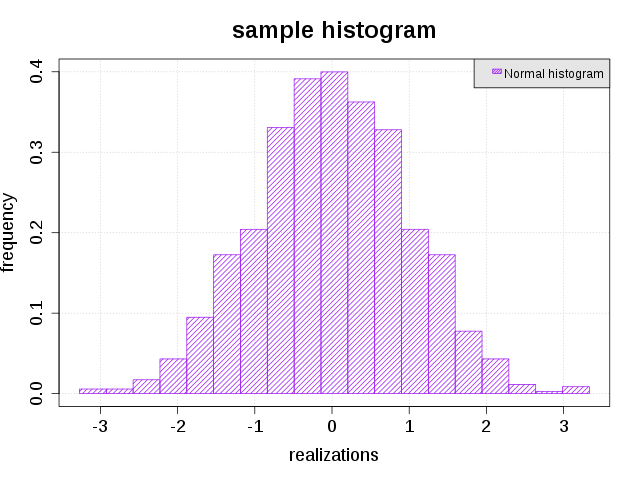
\includegraphics[width=7cm]{Figures/hist_Data.png}
                   \caption{Histogram from a sample.}
                   \label{HistogramData}
                 \end{center}
               \end{minipage}
               \hfill
               \begin{minipage}{9.8cm}
                 \begin{center}
                   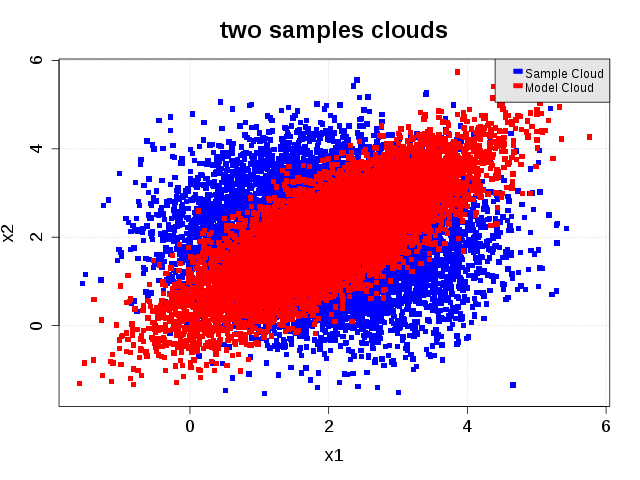
\includegraphics[width=7cm]{Figures/cloud1.png}
                   \caption{Superposition of two 2D clouds.}
                   \label{superpositionTwoclouds}
                 \end{center}
               \end{minipage}
             \end{figure}

\newpage % Copyright 2005-2016 Airbus-EDF-IMACS-Phimeca
% Permission is granted to copy, distribute and/or modify this document
% under the terms of the GNU Free Documentation License, Version 1.2
% or any later version published by the Free Software Foundation;
% with no Invariant Sections, no Front-Cover Texts, and no Back-Cover
% Texts.  A copy of the license is included in the section entitled "GNU
% Free Documentation License".
\renewcommand{\filename}{docUC_InputWithData_TestSameDist.tex}
\renewcommand{\filetitle}{UC : Do two samples have the same distribution : QQ-plot visual test, Smirnov numerical test}

% \HeaderNNIILevel
% \HeaderIILevel
\HeaderIIILevel



\index{Graph!QQ-plot}
\index{Fitting Test!QQ-plot}
\index{Comparison of distribution test!Smirnov}

The objective of this Use Case is to decide whether both samples follow the same distribution or not. \\

To help the decision, OpenTURNS  proposes one visual test and one numerical test :
\begin{itemize}
\item the QQ-plot visual test : Open Turns associates the empirical quantiles of each data from the both numerical samples,

\item the Smirnov test : it tests if both samples (continuous ones only) follow the same distribution. If $F_{n_1}^{*}$ and $F_{n_2}^{*}$ are the empirical cumulative density functions of both samples of size $n_1$ and $n_2$, the Smirnov test evaluates the decision variable :
  \begin{align*}
    D^2 = \displaystyle \sqrt{\frac{n_1n_2}{n_1+n_2}} \sup_{x}|F_{n_1}^{*}(x) - F_{n_2}^{*}(x)|
  \end{align*}
  which tends towards the Kolmogorov distribution. The hypothesis of same distribution is rejected if $D^2$ is too high (depending on the p-value threshold).
\end{itemize}



Details on the QQ-polt and Kolmogorov-Smirnov  tests may be found in the Reference Guide (\extref{ReferenceGuide}{see files Reference Guide - Step B -- Using QQ-plot to compare two samples and Step B -- Comparison of two samples using Kolmogorov-Smirnov test}{stepB}).\\


\requirements{
  \begin{description}
  \item[$\bullet$] two scalar numerical continuous samples : {\itshape sample1, sample2}
  \item[type:]  NumericalSample
  \end{description}
}
             {
               \begin{description}
               \item[$\bullet$] test result : {\itshape resultSmirnov}
               \item[type:] TestResult
               \end{description}
             }

             \textspace\\
             Python script for this UseCase  :

             \inputscript{script_docUC_InputWithData_estSameDist}

\newpage % Copyright (C) 2005-2015 Airbus - EDF - IMACS - Phimeca
% Permission is granted to copy, distribute and/or modify this document
% under the terms of the GNU Free Documentation License, Version 1.2
% or any later version published by the Free Software Foundation;
% with no Invariant Sections, no Front-Cover Texts, and no Back-Cover
% Texts.  A copy of the license is included in the section entitled "GNU
% Free Documentation License".
\renewcommand{\filename}{docUC_InputWithData_IndependenceTest.tex}
\renewcommand{\filetitle}{UC : Are two scalar samples independent : ChiSquared test, Pearson test, Spearman test}

% \HeaderNNIILevel
% \HeaderIILevel
\HeaderIIILevel



\index{Independence Test!ChiSquared test}
\index{Independence Test!Pearson test}
\index{Independence Test!Spearman test}

The objective of this Use Case is to decide whether two samples are independent or not.\\



To help the decision, OpenTURNS proposes the following tests :
\begin{itemize}
\item the ChiSquared test : it tests if both scalar samples (discrete ones only) are independent.\\
  If $n_{ij}$ is the number of values of the sample $i=(1,2)$ in the modality $1 \leq j \leq m$, $\displaystyle n_{i.} = \sum_{j=1}^m n_{ij}$ $\displaystyle n_{.j} = \sum_{i=1}^2 n_{ij}$, and the ChiSquared test evaluates the decision variable :
  \begin{align*}
    D^2 = \displaystyle \sum_{i=1}^2 \sum_{j=1}^m \frac{( n_{ij} - \frac{n_{i.} n_{.j}}{n} )^2}{\frac{n_{i.} n_{.j}}{n}}
  \end{align*}
  which tends towards the $\chi^2(m-1)$ distribution. The hypothesis of independence is rejected if $D^2$ is too high (depending on the p-value threshold).

\item the Pearson test : it tests if there exists a linear relation between two scalar samples which form a gaussian vector (which is equivalent to have a linear correlation coefficient not equal to zero). \\
  If both samples are $\vect{x} = (x_i)_{1 \leq i \leq n}$ and $\vect{y} = (y_i)_{1 \leq i \leq n}$, and $\bar{x} = \displaystyle \frac{1}{n}\sum_{i=1}^n x_i$ and $\bar{y} = \displaystyle \frac{1}{n}\sum_{i=1}^n y_i$, the Pearson test evaluates the decision variable :
  \begin{align*}
    D = \displaystyle \frac{\sum_{i=1}^n (x_i - \bar{x})(y_i - \bar{y})}{\sqrt{\sum_{i=1}^n (x_i - \bar{x})^2\sum_{i=1}^n (y_i - \bar{y})^2}}
  \end{align*}
  The variable $D$ tends towards a $\chi^2(n-2)$, under the hypothesis of normality of both samples. The hypothesis of a linear coefficient equal to 0 is rejected (which is equivalent to the independence of the samples) if D is too high (depending on the p-value threshold).

\item the Spearman test : it tests if there exists a monotonous relation between two scalar samples.\\
  If both samples are $\vect{x} = (x_i)_{1 \leq i \leq n}$ and $\vect{y}= (y_i)_{1 \leq i \leq n}$,, the Spearman test evaluates the decision variable :
  \begin{align*}
    D = \displaystyle 1-\frac{6\sum_{i=1}^n (r_i - s_i)^2}{n(n^2-1)}
  \end{align*}
  where $r_i = rank(x_i)$ and  $s_i = rank(y_i)$. $D$ is such that $\sqrt{n-1}D$ tends towards the gaussian (0,1) distribution.
\end{itemize}




Details on the independence tests  may be found in the Reference Guide (\extref{ReferenceGuide}{see files Reference Guide - Step B --Chi-squared test for independence, Step B -- Pearson correlation test, Step B -- Spearman correlation test}{stepB}).\\


\requirements{
  \begin{description}
  \item[$\bullet$] two continuous scalar numerical samples of dimension 1 : {\itshape contSample1, contSample2 }
  \item[type:]  NumericalSample
  \item[$\bullet$] two discrete scalar numerical sample {\itshape discSample1, discSample2}
  \item[type:] NumericalSample
  \end{description}
}
             {
               \begin{description}
               \item[$\bullet$] tests results : {\itshape resultChiSquared, resultPearson, resultSpearman}
               \item[type:] TestResult
               \end{description}
             }

             \textspace\\
             Python script for this UseCase :

             \inputscript{script_docUC_InputWithData_IndependenceTest}

\newpage % Copyright 2005-2016 Airbus-EDF-IMACS-Phimeca
% Permission is granted to copy, distribute and/or modify this document
% under the terms of the GNU Free Documentation License, Version 1.2
% or any later version published by the Free Software Foundation;
% with no Invariant Sections, no Front-Cover Texts, and no Back-Cover
% Texts.  A copy of the license is included in the section entitled "GNU
% Free Documentation License".
\renewcommand{\filename}{docUC_InputWithData_PearsonSpearmanTests.tex}
\renewcommand{\filetitle}{UC : Particular manipulations of the Pearson and Spearman tests, when the first sample is of dimension superior to 1.}

% \HeaderNNIILevel
% \HeaderIILevel
\HeaderIIILevel


\index{Independence Test!ChiSquared test}
\index{Independence Test!Pearson test}
\index{Independence Test!Spearman test}

The objective of this Use Case is to decide whether two samples follow a monotonous or linear relation in the case where the first sample is of dimension $>1$.\\
The Pearson and Spearman tests are evaluated successively between some (or all) coordinates of the first sample and the second one, which must be of dimension 1.\\


Details on the Pearson and Spearman tests  may be found in the Reference Guide (\extref{ReferenceGuide}{see files Reference Guide - Step B -- Pearson correlation test, Step B -- Spearman correlation test}{stepB}).\\


\requirements{
  \begin{description}
  \item[$\bullet$] one continuous scalar numerical sample of dimension n : {\itshape sample1}
  \item[type:]  NumericalSample
  \item[$\bullet$] one continuous scalar numerical sample of dimension 1 : {\itshape sample2}
  \item[type:]  NumericalSample
  \end{description}
}
             {
               \begin{description}
               \item[$\bullet$] tests results : {\itshape resultPartialPearson, resultFullPearson, resultPartialSpearman, resultFullSpearman}
               \item[type:] TestResultCollection
               \end{description}
             }

             \textspace\\
             Python script for this UseCase :

             \inputscript{script_docUC_InputWithData_PearsonSpearmanTests}

\newpage % Copyright (C) 2005-2015 Airbus - EDF - IMACS - Phimeca
% Permission is granted to copy, distribute and/or modify this document
% under the terms of the GNU Free Documentation License, Version 1.2
% or any later version published by the Free Software Foundation;
% with no Invariant Sections, no Front-Cover Texts, and no Back-Cover
% Texts.  A copy of the license is included in the section entitled "GNU
% Free Documentation License".
\renewcommand{\filename}{docUC_InputWithData_RegressionTest.tex}
\renewcommand{\filetitle}{UC : Regression test between two scalar numerical samples}

% \HeaderNNIILevel
% \HeaderIILevel
\HeaderIIILevel



\index{Regression Linear Model!Rsquared@$R^2$ test}



The objective of this Use Case is to detect a linear relation between two scalar numerical samples. \\



Details on the linear regression model  may be found in the Reference Guide (\extref{ReferenceGuide}{see file Reference Guide - Step B -- Linear regression}{stepB}).\\



\requirements{
  \begin{description}
  \item[$\bullet$] one continuous scalar numerical sample of dimension n : {\itshape Xsample}
  \item[type:]  NumericalSample
  \item[$\bullet$] one continuous scalar numerical sample of dimension 1 : {\itshape Ysample}
  \item[type:]  NumericalSample
  \end{description}
}
             {
               \begin{description}
               \item[$\bullet$] tests results : {\itshape resultPartialRegression, resultFullRegression, resultPartialSpearman, resultFullSpearman}
               \item[type:] TestResultCollection
               \end{description}
             }

             \textspace\\
             Python script for this UseCase :

             \inputscript{script_docUC_InputWithData_RegressionTest}

\newpage % Copyright (C) 2005-2015 Airbus - EDF - IMACS - Phimeca
% Permission is granted to copy, distribute and/or modify this document
% under the terms of the GNU Free Documentation License, Version 1.2
% or any later version published by the Free Software Foundation;
% with no Invariant Sections, no Front-Cover Texts, and no Back-Cover
% Texts.  A copy of the license is included in the section entitled "GNU
% Free Documentation License".
\renewcommand{\filename}{docUC_InputWithData_FittingTests.tex}
\renewcommand{\filetitle}{UC : Distribution fitting tests, numerical and visual validation tests : Chi-squared test, Kolmogorov test, QQ-plot graph}

% \HeaderNNIILevel
% \HeaderIILevel
\HeaderIIILevel



\index{Graph!QQ-plot}
\index{Fitting Test!QQ-plot}
\index{Fitting Test!ChiSquared}
\index{Fitting Test!Kolmogorov}
\index{Fitting Distribution!Parametric method}



The objective of this Use Case is to :
\begin{itemize}
\item perform some parametric fitting tests on a numerical sample in dimension 1, with the maximum likelihood principle or the moment based method,
\item validate these estimations with numerical tests : the Kolmogorov test (continuous distributions) or the Chi -squared test (discrete distributions),
\item validate these estimations with a visual test : the QQ-plot graph.
\end{itemize}

The QQ-plot visual validation test is used with a numerical sample (representing the data) and a distribution (representing the fitted one). For each point of the numerical sample used in the graph, Open Turns evaluates its empirical quantile and associates to it the corresponding quantile from the fitted distribution. \\

Details on the Maximum Likelihood  Principle may be found in the Reference Guide (\extref{ReferenceGuide}{see files Reference Guide - Step B -- Maximum Likelihood  Principle}{stepB}).\\

Details on the Parametric estimators used to evaluate the parameters of the copula may be found in the Reference Guide (\extref{ReferenceGuide}{see files Reference Guide - Step B --  Parametric Estimation}{stepB}).\\

Details on the QQ-polt, Kolmogorov-Smirnov and  Chi-squared tests may be found in the Reference Guide (\extref{ReferenceGuide}{see files Reference Guide - Step B --  Graphical goodness-of-fit tests : QQ-plot and Henry line and Step B -- Kolmogorov-Smirnov goodness-of-fit test}{stepB}).\\


The example here presents :
\begin{itemize}
\item the fitting of a numerical sample of dimension 1 with a Beta distribution, its validation with the Kolmogorov test and the  QQ-Plot graph,
\item the fitting of a numerical sample of dimension 1 with a Poisson distribution, its validation with the Chi-squared test and the  QQ-Plot graph.
\end{itemize}


\requirements{
  \begin{description}
  \item[$\bullet$] a scalar numerical sample (data) : {\itshape sample}
  \item[type:]  NumericalSample
  \end{description}
}
             {
               \begin{description}
               \item[$\bullet$] a Beta and Geometric estimated  distribution : {\itshape estimatedBeta, estimatedGeom}
               \item[type:] Beta, Geometric
               \end{description}

               \begin{description}
               \item[$\bullet$]  results of fitting test : {\itshape resultKolmogorov, resultChiSquared}
               \item[type:] Testresult
               \end{description}
             }

             \textspace\\
             Python script for this UseCase :

             \inputscript{script_docUC_InputWithData_FittingTests}

             \textspace\\


             Figures \ref{qqplotExRight} and \ref{qqplotExFalse} show a QQ-Plot graph to test the adequation of a sample generated  from a Beta(r = 1.2, t = 3.4, a = 1.0, b = 2.0) to :
             \begin{itemize}
             \item the Beta(r = 1.2, t = 3.4, a = 1.0, b = 2.0) distribution : visual validation of the fitting,
             \item the Weibull($\mu$ = 1.5, $\sigma$ = 1.0, $\gamma$ = 1.0) : visual invalidation of the fitting.
             \end{itemize}




             \begin{figure}[H]
               \begin{center}
                 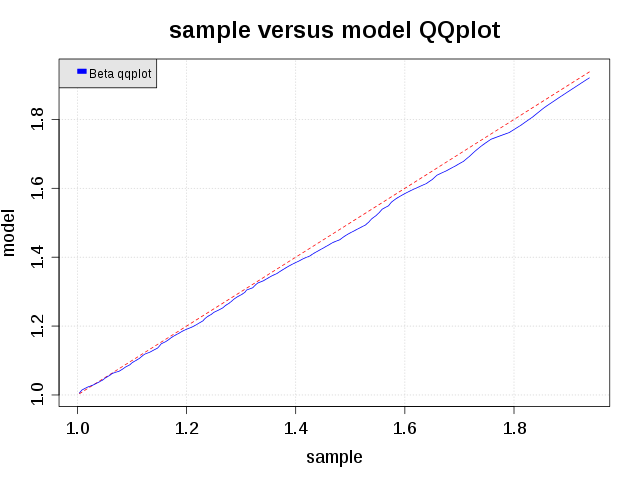
\includegraphics[width=10cm]{Figures/beta_QQplot.png}
               \end{center}
               \caption{Fitting validation by the QQ-Plot graph : Beta fitting to a Beta-sample.}
               \label{qqplotExRight}
             \end{figure}

             \begin{figure}[H]
               \begin{center}
                 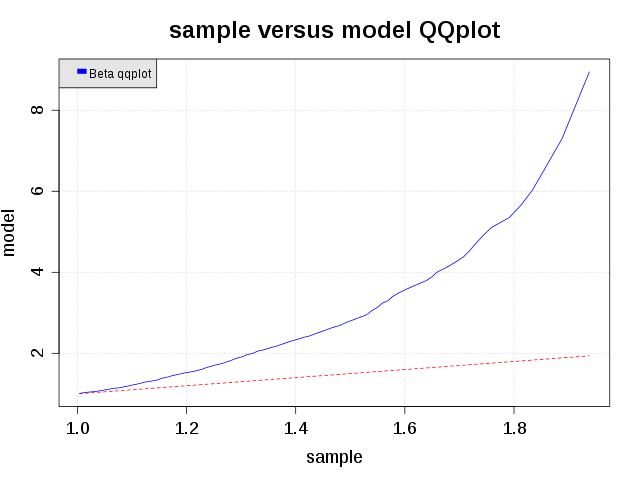
\includegraphics[width=10cm]{Figures/weibull_QQplot.png}
               \end{center}
               \caption{Fitting invalidation by the QQ-Plot graph : Weibull fitting to a Beta sample.}
               \label{qqplotExFalse}
             \end{figure}

\newpage % Copyright (C) 2005-2015 Airbus - EDF - IMACS - Phimeca
% Permission is granted to copy, distribute and/or modify this document
% under the terms of the GNU Free Documentation License, Version 1.2
% or any later version published by the Free Software Foundation;
% with no Invariant Sections, no Front-Cover Texts, and no Back-Cover
% Texts.  A copy of the license is included in the section entitled "GNU
% Free Documentation License".
\renewcommand{\filename}{docUC_InputWithData_NormalFittingTests.tex}
\renewcommand{\filetitle}{UC : Normal distribution fitting test, visual validation tests (Henry line) and numerical validation tests in extreme zones (Anderson Darling test and Cramer Von Mises test)}

% \HeaderNNIILevel
% \HeaderIILevel
\HeaderIIILevel


\index{Fitting Test!Henry line}
\index{Fitting Test!Anderson Darling}
\index{Fitting Test!Cramer Von Mises}
\index{Graph!Henry line}
\index{Graph!QQ-plot}
\index{Graph Manipulation!Bounding box}
\index{Graph Manipulation!View}
\index{Graph Manipulation!Show}

The objective of this Use Case is to fit a normal distribution to a scalar numerical sample, with the maximum likelihood principle or the moment based method, and to validate it with visual and numerical tests.\\

Details on the Maximum Likelihood  Principle may be found in the Reference Guide (\extref{ReferenceGuide}{see files Reference Guide - Step B -- Maximum Likelihood  Principle}{stepB}).\\

Details on the Anderson Darling, Cramer Von Mises and Henry line tests  may be found in the Reference Guide (\extref{ReferenceGuide}{see file Reference Guide - Step B -- Anderson Darling goodness-of-fit test, Step B -- Cramer Von Mises goodness-of-fit test and Step B -- Graphical goodness-of-fit tests : QQ-plot and Henry line}{stepB}).\\


To help this decision,  OpenTURNS proposes the following tests :
\begin{itemize}
\item the Henry line visual test, which is the QQ-Plot graph adapted to the normal distribution,
\item the Anderson Darling test : this test gives more importance to extreme values. If $F_n$ is the empirical cumulative density function of the sample $(x_i)_{1 \leq i \leq n}$ and if $(x_{(i)})_{1 \leq i \leq n}$ is the ordered sample, the Anderson Darling test evaluates the decision variable :
  \begin{align*}
    \begin{array}{lcl}
      AD^2 & = & \displaystyle  n \int_{\Rset} \frac{(F_n(x) - F(x))^2}{f(x)(1-F(x))} dF(x)\\
      & = &  \displaystyle -n -\frac{1}{n} \sum_{i=1}^{n} (2i-1)[\log(f(x_{(i)})) + \log(1-F(x_{(n-i+1)}))]
    \end{array}
  \end{align*}
  Under the hypothesis of normality of the distribution $F$, the decision variable has a tabulated distribution.
\item the Cramer Von Mises test : this test gives also more importance to extreme values. If $F_n$ is the empirical cumulative density function of the sample $(x_i)_{1 \leq i \leq n}$ and if $(x_{(i)})_{1 \leq i \leq n}$ is the ordered sample, the Cramer Von Mises test evaluates the decision variable :
  \begin{align*}
    \begin{array}{lcl}
      CM & = & \displaystyle  \int_{\Rset}(F_n(x) - F(x))^2dF(x)\\
      & = &  \displaystyle \frac{1}{12n} + \sum_{i=1}^{n} \left[\frac{2i-1}{2n} - F(x_{(i)}) \right]^2
    \end{array}
  \end{align*}
  Under the hypothesis of normality of the distribution $F$, the decision variable has a tabulated distribution.
\end{itemize}

\requirements{
  \begin{description}
  \item[$\bullet$] a scalar numerical sample (data)  : {\itshape sample}
  \item[type:]  NumericalSample
  \end{description}
}
             {
               \begin{description}
               \item[$\bullet$] a normal fitted distribution : {\itshape estimatedNormalDistribution}
               \item[type:]  Distribution
               \item[$\bullet$] the files containing the Henry line graph : {\itshape HenryPlot.png, HenryPlot.eps}
               \item[type:] files at format PNG or EPS or FIG
               \item[$\bullet$] a numerical validation by the Anderson Darling test for two continuous distributions (p-value)
               \item[type:] TestResult
               \item[$\bullet$] a numerical validation by the  test for Cramer Von Mises discrete distribution (p-value)
               \item[type:] TestResult
               \end{description}
             }

             \textspace\\
             Python script for this UseCase :

             \inputscript{script_docUC_InputWithData_NormalFittingTests}

             \textspace\\

             Figures \ref{henryLineExRight} and \ref{henryLineExFalse} show the Henry Line of a sample coming from a  :
             \begin{itemize}
             \item  Normal($\mu$ = 0.0, $\sigma$ = 1.0) distribution : visual validation of the normality,
             \item  Beta(r = 0.7, t = 1.6, a = 0.0, b = 2.0) distribution : visual invalidation of the normality.
             \end{itemize}



             \begin{figure}[H]
               \begin{minipage}{10cm}
                 \begin{center}
                   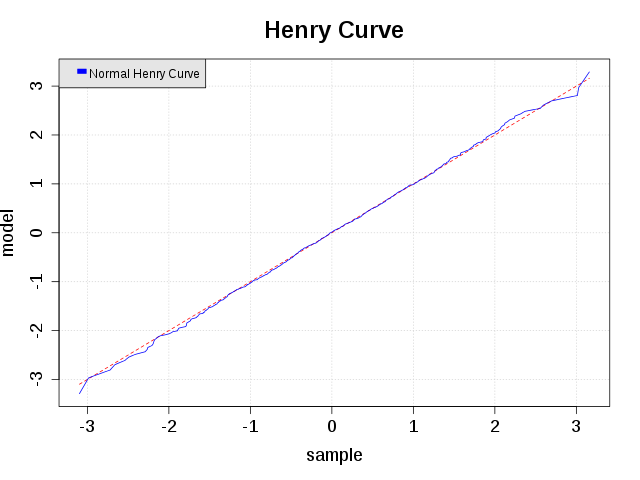
\includegraphics[width=7cm]{Figures/HenryLineTestRight.png}
                   \caption{Validation of the hypothesis of normality by the Henry Line for a Normal-sample.}
                   \label{henryLineExRight}
                 \end{center}
               \end{minipage}
               \hfill
               \begin{minipage}{10cm}
                 \begin{center}
                   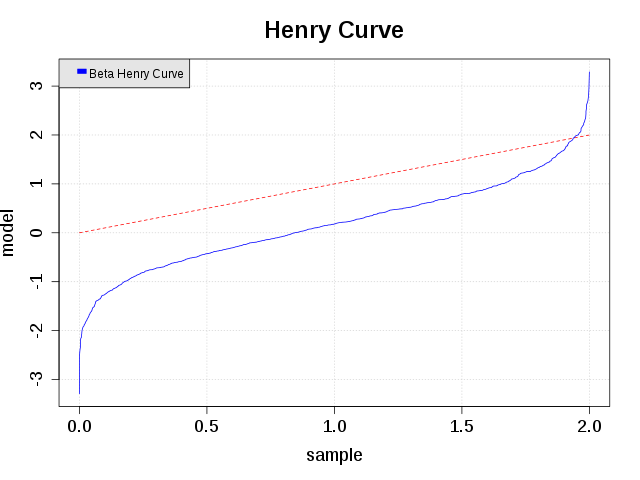
\includegraphics[width=7cm]{Figures/HenryLineTestFalse.png}
                   \caption{Invalidation of the hypothesis of normalityHenry Line for a Beta-sample.}
                   \label{henryLineExFalse}
                 \end{center}
               \end{minipage}
             \end{figure}

\newpage % Copyright 2005-2016 Airbus-EDF-IMACS-Phimeca
% Permission is granted to copy, distribute and/or modify this document
% under the terms of the GNU Free Documentation License, Version 1.2
% or any later version published by the Free Software Foundation;
% with no Invariant Sections, no Front-Cover Texts, and no Back-Cover
% Texts.  A copy of the license is included in the section entitled "GNU
% Free Documentation License".
\renewcommand{\filename}{docUC_InputWithData_ChoiceFittedDistributions.tex}
\renewcommand{\filetitle}{UC : Making a choice between multiple fitted distributions :  Kolmogorov ranking, ChiSquared ranking and BIC ranking}

% \HeaderNNIILevel
% \HeaderIILevel
\HeaderIIILevel



\index{Ranking test!Kolmogorov}
\index{Ranking test!ChiSquared}
\index{Ranking test!BIC}

The objective of this Use Case is to help to make a choice between several distributions fitted to a numerical sample. This choice can be motivated by :
\begin{itemize}
\item the ranking by the Kolmogorov p-values (for continuous distributions),
\item the ranking by the ChiSquared p-values (for discrete distributions),
\item the ranking BIC values.
\end{itemize}


Details on the BIC criterion may be found in the Reference Guide (\extref{ReferenceGuide}{see file Reference Guide - Step B -- Bayesian Information Criterion (BIC)}{stepB}).\\

It does not  require to  specify the parameters of the different models tested. It is possible to precise :
\begin{itemize}
\item the model only : in that case, OpenTURNS builds a factory for each model. OpenTURNS first evaluates  the parameters of the distribution (through the maximum likelihood rule or the moment based one) and then  ranks the distributions according to the criteria selected,
\item the complete distributions with their parameters : OpenTURNS only evaluates the selected criteria  on each of them and rank them.
\end{itemize}
Note that it is possible to specify a KernelSmoothing distribution in the list of the models tested.

\textspace\\

\requirements{
  \begin{description}
  \item[$\bullet$] some continupous or discrete numerical samples (data) :  {\itshape sample\_cont, sample\_dist}
  \item[type:]  NumericalSample
  \end{description}
}
             {
               \begin{description}
               \item[$\bullet$] a continuous distribution which ranks first by the Kolmogorov test  : {\itshape bestContModelKol, bestcontDistKol}
               \item[type:] Distribution
               \item[$\bullet$] a continuous distribution which ranks first by the BIC test  : {\itshape bestContModelBIC}
               \item[type:] Distribution
               \item[$\bullet$] a discrete distribution which ranks first by the Chi Squared test  : {\itshape bestDiscModelChiSq}
               \item[type:] Distribution
               \item[$\bullet$] a discrete distribution which ranks first by the BIC  test  : {\itshape bestDiscDistBIC}
               \item[type:] Distribution
               \end{description}
             }

             \textspace\\
             Python script for this UseCase :

             \inputscript{script_docUC_InputWithData_ChoiceFittedDistributions}

\newpage % Copyright 2005-2016 Airbus-EDF-IMACS-Phimeca
% Permission is granted to copy, distribute and/or modify this document
% under the terms of the GNU Free Documentation License, Version 1.2
% or any later version published by the Free Software Foundation;
% with no Invariant Sections, no Front-Cover Texts, and no Back-Cover
% Texts.  A copy of the license is included in the section entitled "GNU
% Free Documentation License".
\renewcommand{\filename}{docUC_InputWithData_KernelSmoothing.tex}
\renewcommand{\filetitle}{UC : PDF fitting by kernel smoothing and graphical validation : superposition of the empirical and kernel smoothing CDF}

% \HeaderNNIILevel
% \HeaderIILevel
\HeaderIIILevel


\index{Distribution!Kernel mixture}
\index{Fitting Distribution!Kernel smoothing}
\index{Graph!Empirical cumulative density function}
\index{Graph!PDF-CDF curves}
\index{Graph!Superposition empirical - kernel smoothed CDF}

The objective of this Use Case is to model the PDF of a random  vector, described by a numerical sample thanks to the kernel smoothing method and to superpose on the same graph the kernel smoothing PDF and the histogram built from the same numerical sample.\\



Details on the kernel smoothing method may be found in the Reference Guide (\extref{ReferenceGuide}{see file Reference Guide - Step B -- Kernel Smoothing}{stepB}).\\


In dimension 1, the kernel smoothed probability density function $\hat{p}$ has the following expression, where $K$ is the univariate kernel, $n$ the numerical sample size and $(X_1, \cdots, X_n) \in \Rset^n$ the univariate random sample with $\forall i, \, \, X_i \in \Rset$ :
\begin{equation}
  \label{kernelSmooth}
  \hat{p}(x) = \displaystyle \frac{1}{nh}\sum_{i=1}^{n} K\left(\frac{x-X_i}{h}\right)
\end{equation}
The kernel $K$ is a function satisfying $\int K(x)\, dx=1$. Usually, $K$ is chosen to be a unimodal probability density function that is symmetric about 0.\\
The parameter $h$ is called the \emph{bandwidth}.\\

 In dimension $d>1$, OpenTURNS uses the product kernel $K_d$, defined by: 
  \begin{align*}
    K_d(\vect{x}) = \displaystyle \prod_{j=1}^{d} K(x_j)
  \end{align*}
 where $\vect{x} = (x_1, \cdots, x_d)\in \Rset^d$. Thus, the kernel smoothed probability density function in dimension $d$ writes:
  \begin{align*}
    \hat{p}(\vect{x}) = \displaystyle \frac{1}{N \prod_{j=1}^{d}h_j} \sum_{i=1}^{N} K_d\left(\frac{x_1 - X_{i1} }{h_1}, \dots, \frac{x_d - X_{id}}{h_d}\right)
  \end{align*}
where $(\vect{X}_1, \cdots, \vect{X}_n)$ is the d-variate random  sample which components are denoted $\vect{X}_i = (X_{i1}, \dots, X_{id})$. \\
  Let's note that the bandwidth is the vector $\vect{h} = (h_1, \cdots, h_d)$. \\
The default kernel of OpenTURNS is the product of standard Normal distributions. The dimension of the product is automatically evaluated from the random sample.\\

In dimension 1, the boundary effects may be taken into account in OpenTURNS : the boundaries are automatically detected from the numerical sample (with the \textit{min} and \textit{max} functions) and the kernel smoothed PDF is corrected in the boundary areas to remain within the boundaries, according to the miroring technique :
\begin{itemize}
\item the Scott bandwidth is evaluated from the numerical sample : $h$
\item two subsamples are extracted from the inital numerical sample, containing all the points within the range $[min, min + h[$ and  $]max-h, max]$,
\item both subsamples are transformed into their symmetric samples with respect their respective boundary : its results two samples within the range  $]min-h, min]$ and  $[max, max+h[$,
      \item a kernel smoothed PDF is built from the new numerical sample composed with the initial one and the two new ones, with the previous bandwidth $h$,
      \item this last kernel smoothed PDF is truncated within the inital range  $[min, max]$ (conditional PDF).
\end{itemize}
\vspace*{0.1cm}

The choice of the kind of the kernel is free in OpenTURNS : it is possible to select any 1D distribution and to define it as a kernel. However, in order to optimize the efficiency of the kernel smoothing fitting (it means to minimise the AMISE error), it is recommended to select a {\bf symmetric distribution} for the kernel. \\
All the distribution default constructors of OpenTURNS create a symmetric default distribution when possible. It is also possible to work with the Epanechnikov kernel, which is a $Beta(r=2, t=4, a=-1, b=1)$. \\

The bandwidth $\vect{h}$ may be fixed by the User. However, it is recommended to let OpenTURNS evaluate it automatically from the numerical sample according to the following rules :
\begin{itemize}
\item In dimension $d$, OpenTURNS automatically applies the Scott rule.
\item In dimension 1, the automatic bandwidth selection method depends  on the size $n$ of the numerical sample. As a matter of fact, the computation bottleneck is the estimation of the estimators $\hat{\Phi}_r$ as it requires the evaluation of a double summation on the numerical sample, which has a cost of $\cO(n^2)$.
  \begin{itemize}
  \item if $n \leq 250$, the Solve-the-equation  plug-in method is used on the entire numerical sample.
  \item if $n>250$, the Solve-the-equation  plug-in method is too computationnally expensive. Then, OpenTURNS proceeds as follows :the plug-in method on the entire numerical sample if its size is inferior to 250; the mixted method in the other case. Refer to the Reference Guide for more details on these methods.
  \end{itemize}
\end{itemize}


It is possible to specify a particular bandwidth, evaluated according to one of the previous rules as follows :
\begin{itemize}
\item \emph{computeSilvermanBandwidth} applies the Silverman rule,
\item \emph{computePluginBandwidth} applies the plug-in method on the entire numerical sample,
\item \emph{computeMixedBandwidth} applies the mixted plug-in method on the entire numerical sample, as described above.
\end{itemize}

\textspace\\
\requirements{
  \begin{description}
  \item[$\bullet$] a nD-sample : {\itshape sample}
  \item[type:]  NumericalSample
  \end{description}
}
             {
               \begin{description}
               \item[$\bullet$] a kernel smoothed distribution : {\itshape kernelSmoothedDist}
               \item[type:]  Distribution
               \end{description}
             }

             \textspace\\
             Python script for this UseCase :

             \inputscript{script_docUC_InputWithData_KernelSmoothing}

             \textspace\\


             Figures \ref{pdf_KernelSmooth} and \ref{cdf_KernelSmooth}  show a 1D kernel smoothing of a distribution of type Mixture which PDF is defined by : 0.2*Triangular(1.0, 2.0, 4.0) + 0.5*Normal(-1.0, 1.0) + 0.3*Exponential(1.0, 3.0), thanks to a numerical sample of size $10^4$, with a Normal,  Triangular and Epanechnikov kernel, when the  bandwidth is selected according to the mixted plug-in method.\\

             Figures \ref{pdf_KernelSmoothBWSel} and \ref{cdf_KernelSmoothBWSel} show the difference when the previous distribution is estimated with  a Normal kernel and when the bandwidth is selected according to the Silverman rule, the plug-in method or the mixted plug-in method, thanks to a numerical sample of size $10^3$.\\

             Figures \ref{pdf_KernelSmooth_boundary} and \ref{cdf_KernelSmooth_boundary} show the effect of the boundary treatment in the kernel smoothing through the example of the exponential distribution $Exp(\lambda = 2.0, \gamma = 0.0)$. A Normal kernel is used and the  bandwidth is selected according to the mixted plug-in method, thanks to a numerical sample of size $10^4$.


             \begin{figure}[H]
               \begin{minipage}{7cm}
                 \begin{center}
                   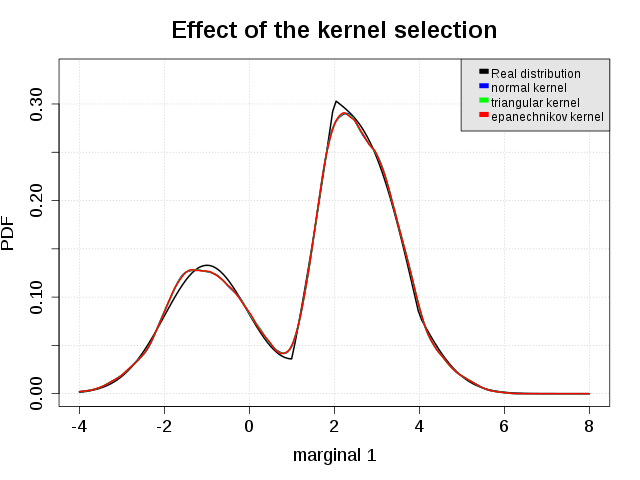
\includegraphics[width=7cm]{Figures/kernelSmoothing_pdf.png}
                   \caption{PDF of th kernel smoothed distribution and of the real one with different kernels.}
                   \label{pdf_KernelSmooth}
                 \end{center}
               \end{minipage}
               \hfill
               \begin{minipage}{7cm}
                 \begin{center}
                   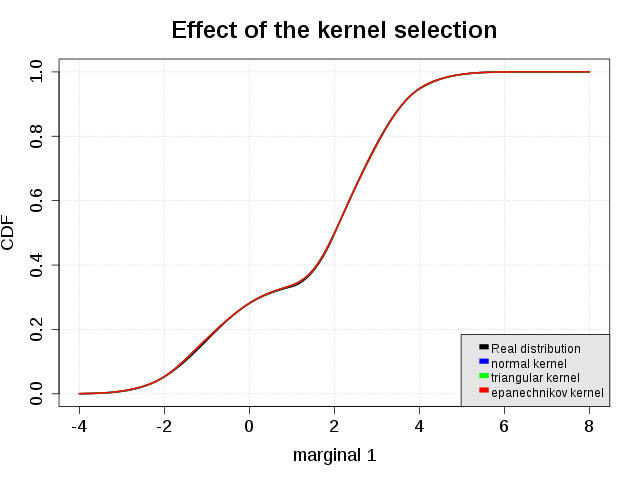
\includegraphics[width=7cm]{Figures/kernelSmoothing_cdf.png}
                   \caption{CDF of the kernel smoothed distribution and of the real one with different kernels.}
                   \label{cdf_KernelSmooth}
                 \end{center}
               \end{minipage}
             \end{figure}


             \begin{figure}[H]
               \begin{minipage}{7cm}
                 \begin{center}
                   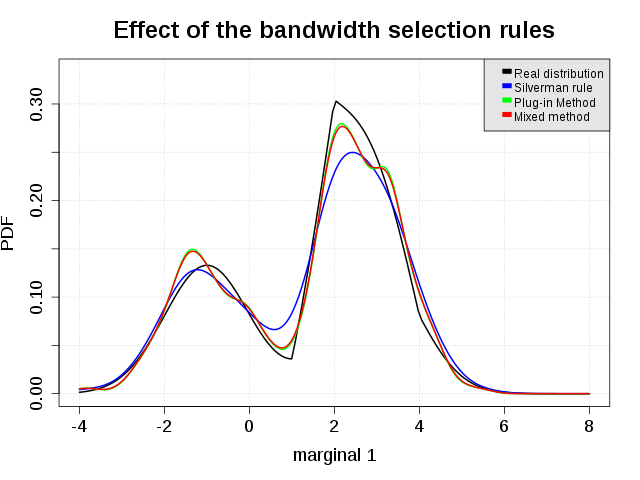
\includegraphics[width=7cm]{Figures/kernelSmoothingBWSel_pdf.png}
                   \caption{PDF of the kernel smoothed distribution and of the real one with different bandwidth selection rules.}
                   \label{pdf_KernelSmoothBWSel}
                 \end{center}
               \end{minipage}
               \hfill
               \begin{minipage}{7cm}
                 \begin{center}
                   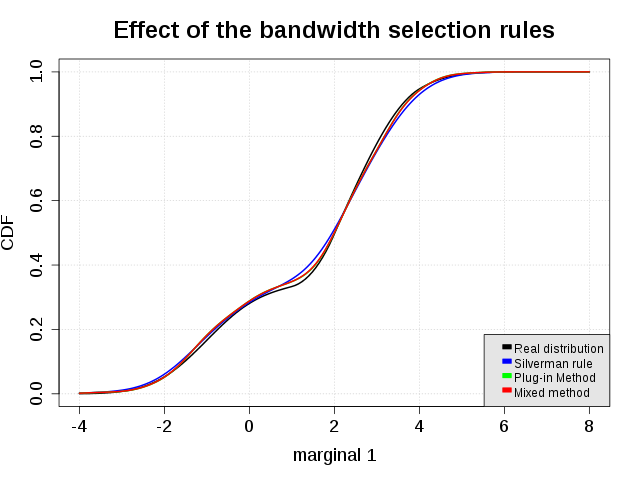
\includegraphics[width=7cm]{Figures/kernelSmoothingBWSel_cdf.png}
                   \caption{CDF of the kernel smoothing distributions and of the real one with different bandwidth selection rules.}
                   \label{cdf_KernelSmoothBWSel}
                 \end{center}
               \end{minipage}
             \end{figure}

             \begin{figure}[H]
               \begin{minipage}{7cm}
                 \begin{center}
                   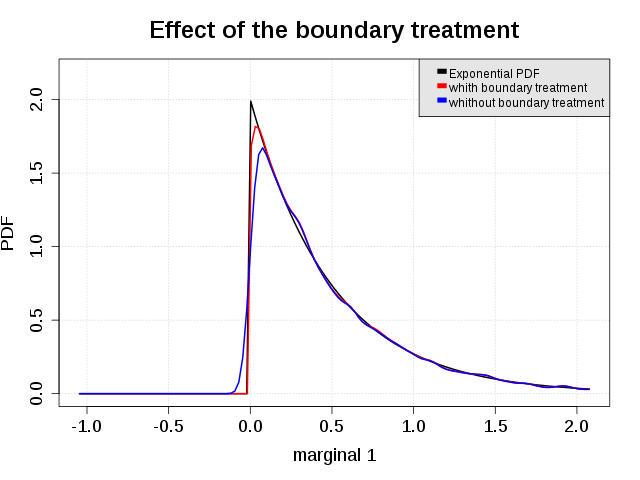
\includegraphics[width=7cm]{Figures/kernelSmoothing_boundary_pdf.png}
                   \caption{Effect of the boundary treatment on the kernel smoothing PDF of an exponential distribution.}
                   \label{pdf_KernelSmooth_boundary}
                 \end{center}
               \end{minipage}
               \hfill
               \begin{minipage}{7cm}
                 \begin{center}
                   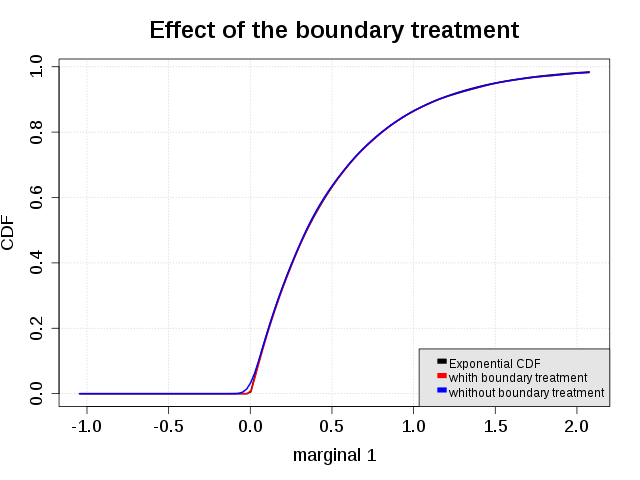
\includegraphics[width=7cm]{Figures/kernelSmoothing_boundary_cdf.png}
                   \caption{Effect of the boundary treatment on the kernel smoothing CDF of an exponential distribution.}
                   \label{cdf_KernelSmooth_boundary}
                 \end{center}
               \end{minipage}
             \end{figure}

\newpage % Copyright (C) 2005-2015 Airbus - EDF - IMACS - Phimeca
% Permission is granted to copy, distribute and/or modify this document
% under the terms of the GNU Free Documentation License, Version 1.2
% or any later version published by the Free Software Foundation;
% with no Invariant Sections, no Front-Cover Texts, and no Back-Cover
% Texts.  A copy of the license is included in the section entitled "GNU
% Free Documentation License".
\renewcommand{\filename}{docUC_InputNoData_CopulaEstimation.tex}
\renewcommand{\filetitle}{UC : Estimation of a Copula from a sample}

% \HeaderNNIILevel
% \HeaderIILevel
\HeaderIIILevel


\label{copula_estimation}


\index{Copula!Estimation from a sample}
\index{Graph Manipulation!Bounding box}
\index{Graph Manipulation!View}
\index{Graph Manipulation!Show}
\index{Fitting Test!QQ-plot}
\index{Fitting Distribution!Parametric method}



The objective of this Use Case is to :
\begin{itemize}
\item fit a copula to a sample : this estimation may be parametric (when using a specific model of copula) or not (when using the Sklar Copula extracted from a non parametric estimation of the multivariate distribution),
\item validate the estimation with a visual test by superposing the iso-curves of the estimated copula and the sample in the rank space.
\end{itemize}


Details on the Maximum Likelihood  Principle may be found in the Reference Guide (\extref{ReferenceGuide}{see files Reference Guide - Step B -- Maximum Likelihood  Principle}{stepB}).\\

Details on the Parametric Estimators used to evaluate the parameters of the copula may be found in the Reference Guide (\extref{ReferenceGuide}{see files Reference Guide - Step B --  Parametric Estimation}{stepB}).\\



\requirements{
  \begin{description}
  \item[$\bullet$] a 2D numerical sample (data) : {\itshape sample}
  \item[type:]  NumericalSample
  \end{description}
}
             {
               \begin{description}
               \item[$\bullet$] some estimations of the copula : {\itshape estimatedParamCop,estimatedSklarCop }
               \item[type:] a Copula
               \end{description}
             }

             \textspace\\
             Python script for this UseCase :

             \inputscript{script_docUC_InputWithData_CopulaEstimation}

             \textspace\\


             Figure \ref{InitCloud} draws the cloud of the sample in the physical  space and  Figure \ref{RankCloud} draws the sample in the rank space. Figure \ref{Superposition} draws the superposition of the sample in the rank space and the iso-curves of the estimated copula.



             \begin{figure}[H]
               \begin{minipage}{10cm}
                 \begin{center}
                   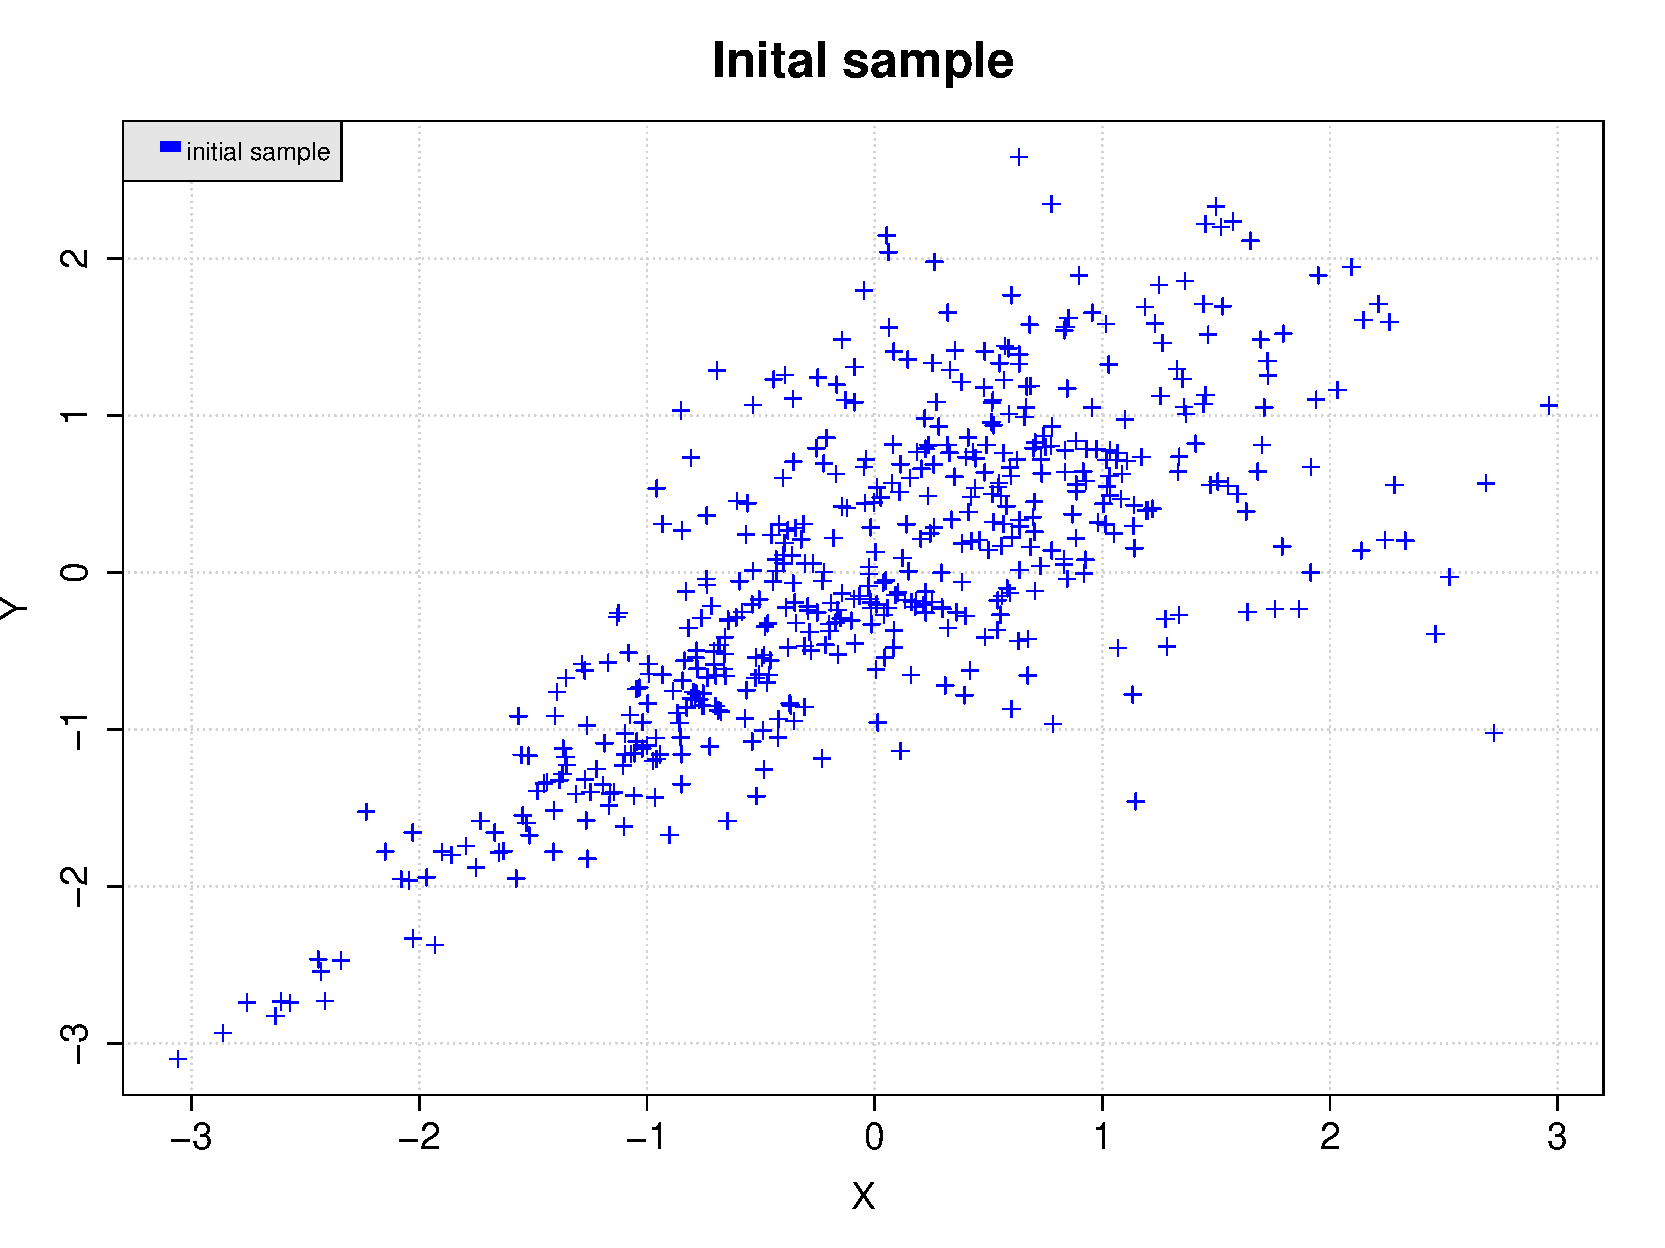
\includegraphics[width=10cm]{Figures/initSample.pdf}
                 \end{center}
                 \caption{Initial sample.}
                 \label{InitCloud}
               \end{minipage}
               \hfill
               \begin{minipage}{10cm}
                 \begin{center}
                   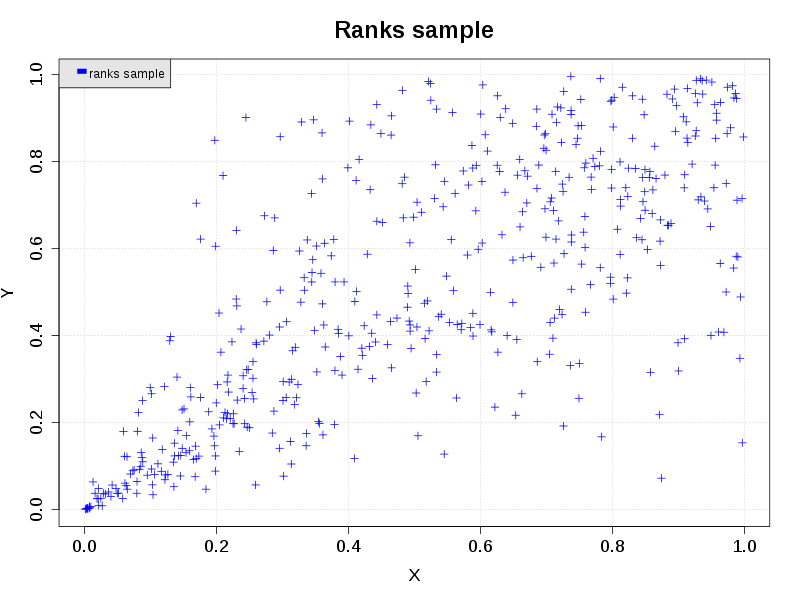
\includegraphics[width=10cm]{Figures/ranksSample.png}
                 \end{center}
                 \caption{Sample in the rank space.}
                 \label{RankCloud}
               \end{minipage}
             \end{figure}


             \begin{figure}[H]
               \begin{center}
                 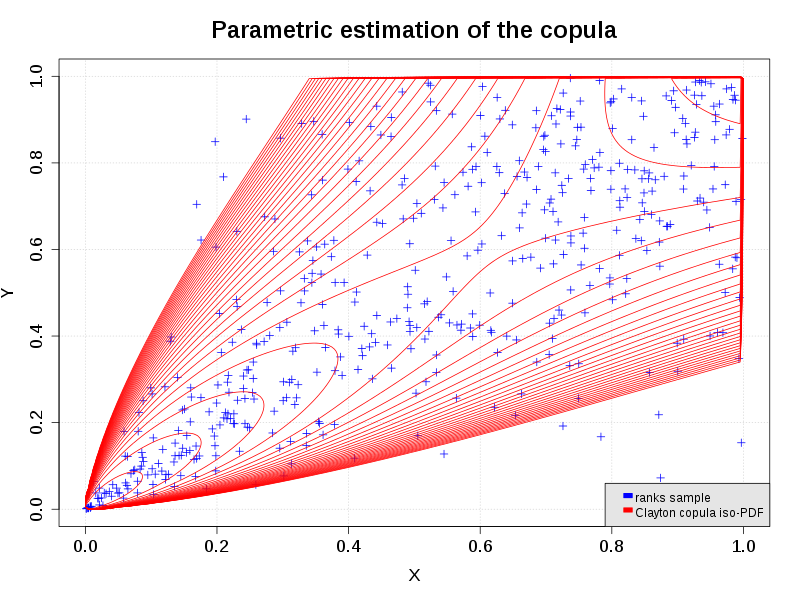
\includegraphics[width=10cm]{Figures/copula_estimation.png}
               \end{center}
               \caption{Sample and iso-PDF curves of the estimated copula.}
               \label{Superposition}
             \end{figure}

\newpage % Copyright (C) 2005-2015 Airbus - EDF - IMACS - Phimeca
% Permission is granted to copy, distribute and/or modify this document
% under the terms of the GNU Free Documentation License, Version 1.2
% or any later version published by the Free Software Foundation;
% with no Invariant Sections, no Front-Cover Texts, and no Back-Cover
% Texts.  A copy of the license is included in the section entitled "GNU
% Free Documentation License".
\renewcommand{\filename}{docUC_InputWithData_CopulaKendallPlotTest.tex}
\renewcommand{\filetitle}{UC : Copula validation through the Kendall Plot Test}

% \HeaderNNIILevel
% \HeaderIILevel
\HeaderIIILevel


\label{copula_validation}


\index{Copula!Model Validation}
\index{Fitting Test!Kendall-plot}



The objective of this Use Case is to exhibit the different uses of the Kendall Plot to :
\begin{itemize}
\item test a specific model of bivariate copula with respect to a sample,
\item test whether two bivariate samples share the same copula model.
\end{itemize}


Details on the Kendall Plot Test may be found in the Reference Guide (\extref{ReferenceGuide}{see files Reference Guide - Step B -- Graphical googness-of-fit tests : QQ-plot, Kendall Plot and henry line.}{stepB}).\\


This Use Case performs the following analysis :

In the example, we suppose we have a sample of dimension 2. The objective is to estimate the dependence structure of the sample. The analysis  has the following steps :
\begin{enumerate}
\item  we suppose we have a sample of dimension 2 $sample1$ and a given model of copula \textit{copula} , whatever the way it has been determined (parametric estimation or non parametric one). We want to validate this copula model with the Kendall Plot test, thanks to the method \emph{VisualTest.DrawKendallPlot(sample1, copula)};
\item we suppose we have two samples of dimension 2 $sample1$ and $sample2$. We wonder whether this two samples have the same copula model, whithout specifying it, using the Kendall Plot test, thanks to the method \emph{VisualTest.DrawKendallPlot(sample1, sample2)}.
\end{enumerate}

In OpenTURNS, the mean of the statistics $W_i$ is evaluated with the Monte Carlo sampling method from $n$ simulations. By default, $n=100$. It is possible to change this value thanks to the \textit{ResourceMap} class (see the python script).


\requirements{
  \begin{description}
  \item[$\bullet$] two 2D numerical sample (data) : {\itshape sample1, sample2}
  \item[type:]  NumericalSample
  \end{description}
}
             {
               \begin{description}
               \item[$\bullet$] a bivariate copula : {\itshape copula}
               \item[type:] CopulaImplementation
               \end{description}
             }

             \textspace\\
             Python script for this UseCase :

             \inputscript{script_docUC_InputWithData_CopulaKendallPlotTest}

             \textspace\\

             In Figures  \ref{GoodCop} to \ref{DifCop}, the data 1 and data 2  have been generated from a $Frank(1.5)$ copula, and data 3 from a $Gumbel(4.5)$ copula.\\
             Figures \ref{GoodCop} and \ref{BadCop} respectively validates and invalidates the \textit{Frank} copula model to data 1 and data 2.\\
             Figures \ref{SameCop} and  \ref{DifCop} respectively validates that data 1 and data 2 share the same copula, and shows that data 1 and data 3 don't share the same copula.\\


             \begin{figure}[H]
               \begin{minipage}{10cm}
                 \begin{center}
                   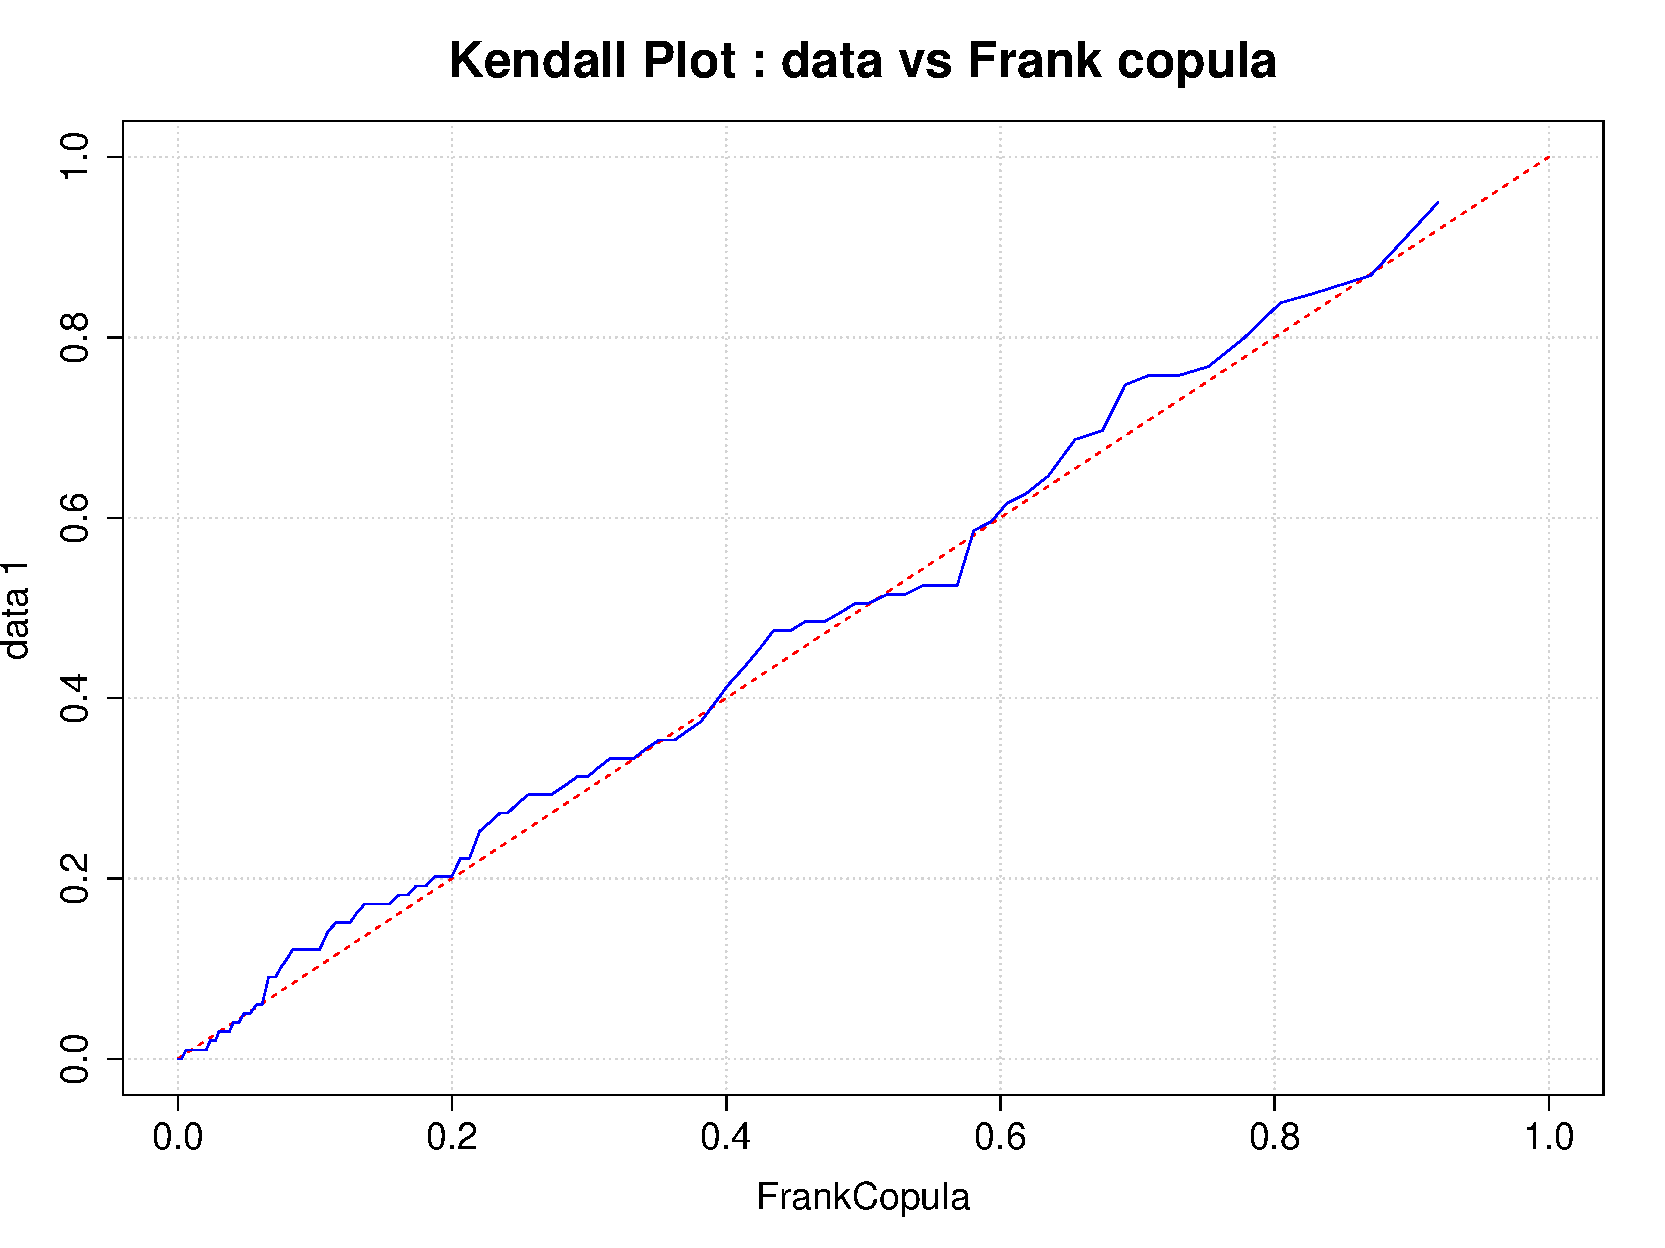
\includegraphics[width=10cm]{Figures/KendallPlotCopula.pdf}
                 \end{center}
                 \caption{The Kendall Plot test validates the use of the Frank copula model for the data 1.}
                 \label{GoodCop}
               \end{minipage}
               \hfill
               \begin{minipage}{10cm}
                 \begin{center}
                   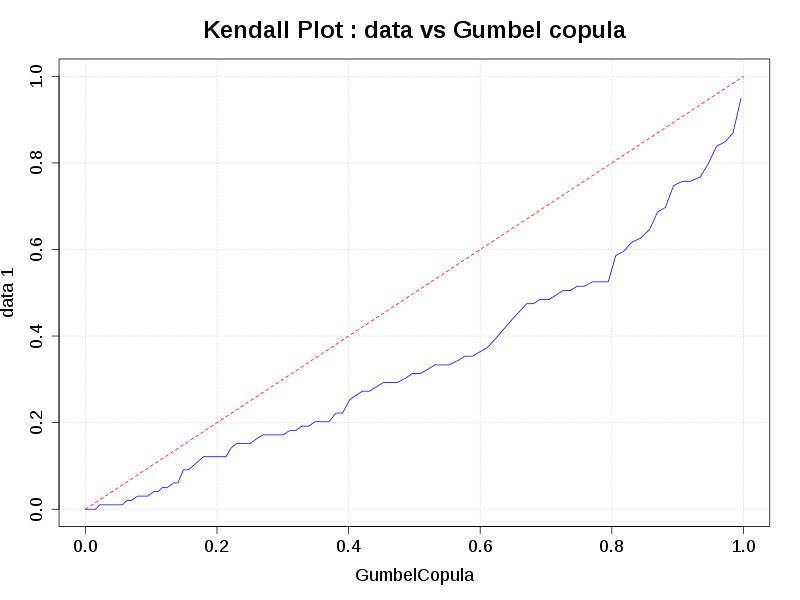
\includegraphics[width=10cm]{Figures/KendallPlotCopulaBad.png}
                 \end{center}
                 \caption{The Kendall Plot test invalidates the use of the Frank copula model for the data 1.}
                 \label{BadCop}
               \end{minipage}
             \end{figure}


             \begin{figure}[H]
               \begin{minipage}{10cm}
                 \begin{center}
                   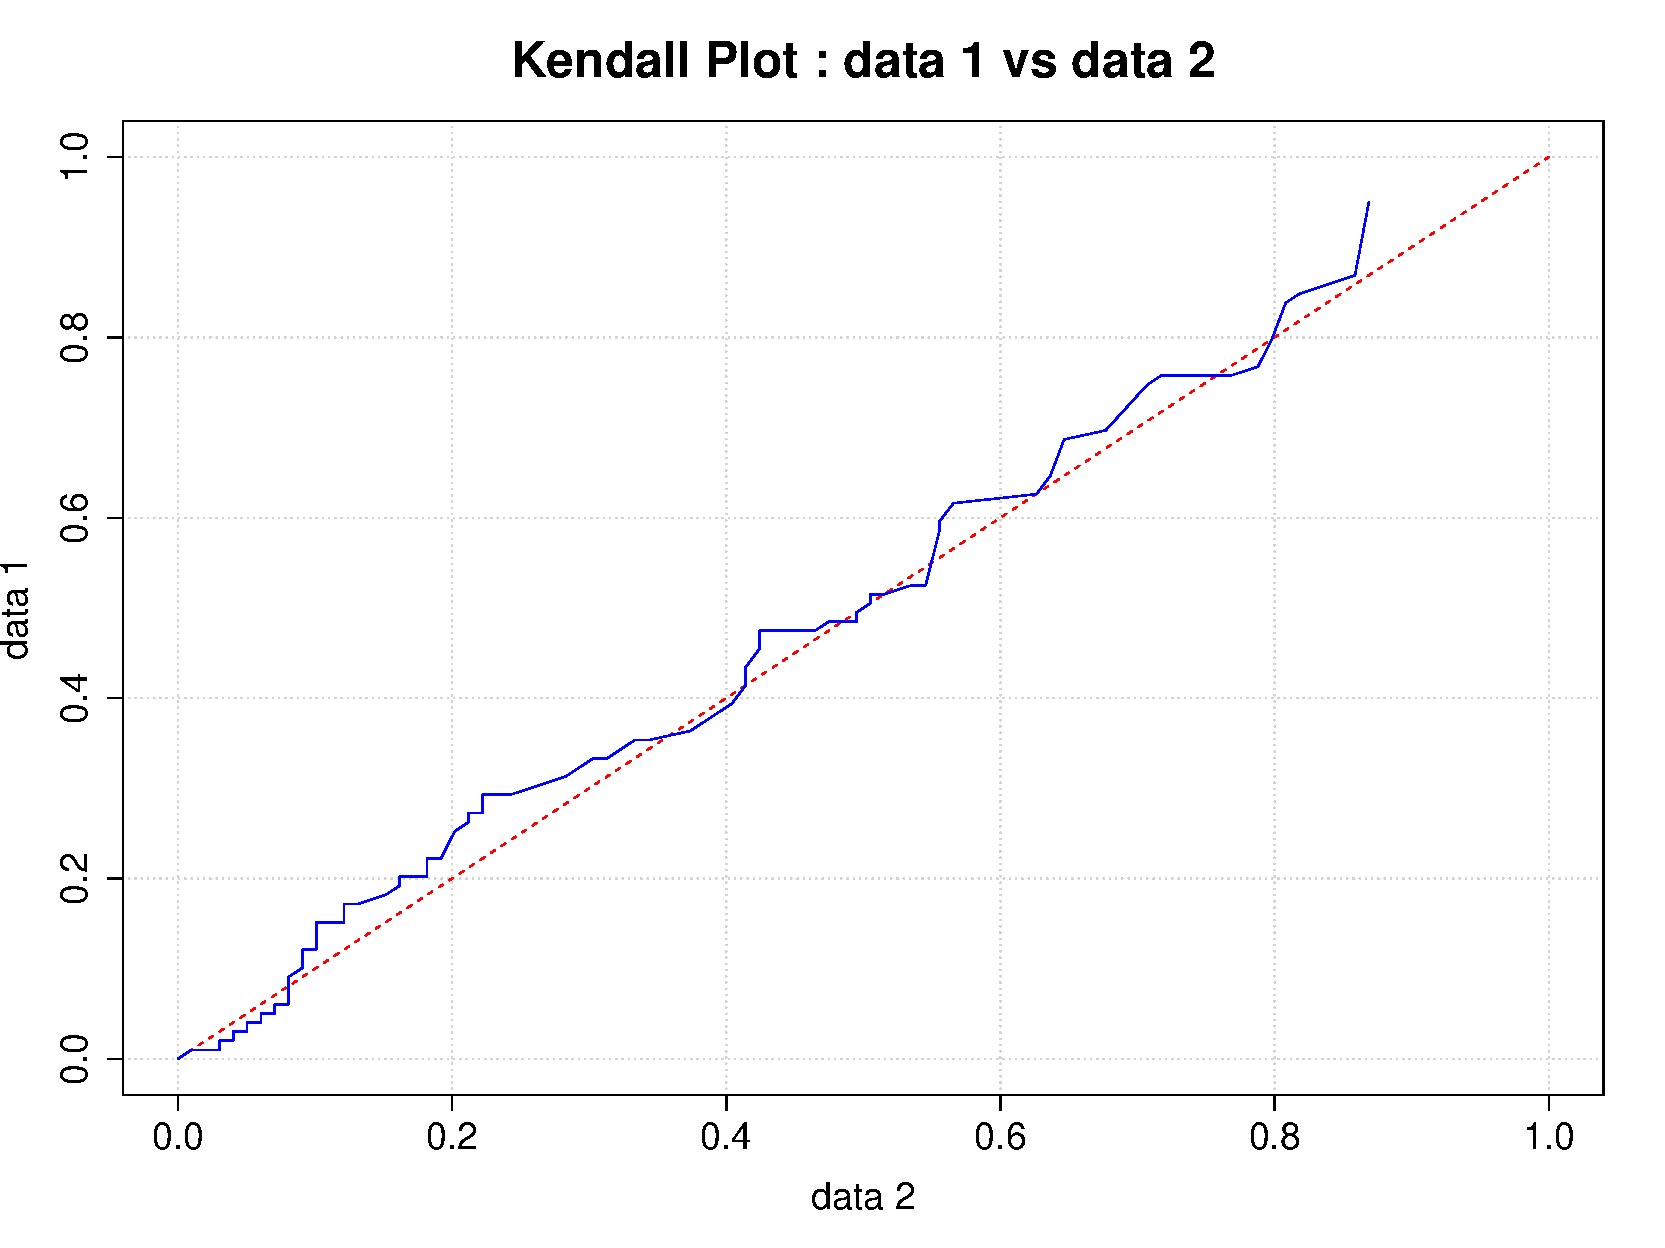
\includegraphics[width=10cm]{Figures/KendallPlotSample.pdf}
                 \end{center}
                 \caption{The Kendall Plot test validates that data 1 and data 2 have the same copula model}.
                 \label{SameCop}
               \end{minipage}
               \hfill
               \begin{minipage}{10cm}
                 \begin{center}
                   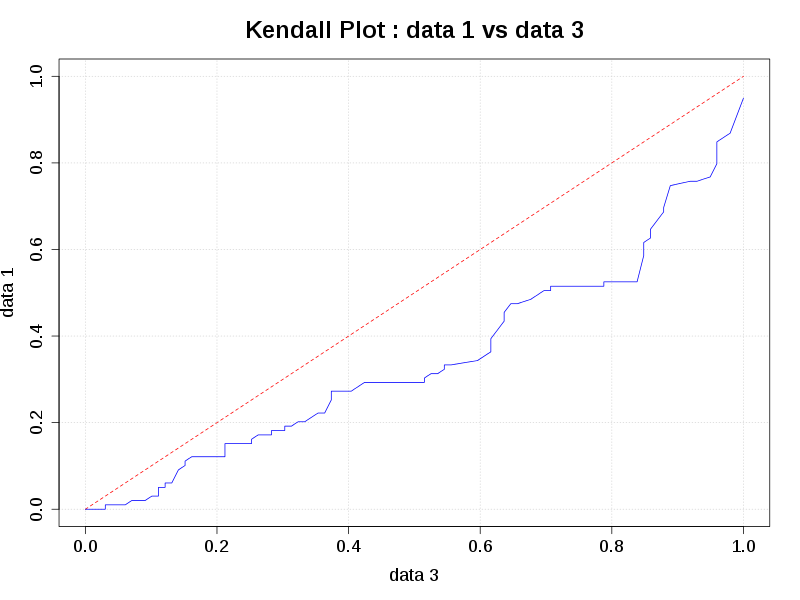
\includegraphics[width=10cm]{Figures/KendallPlotSampleBad.png}
                 \end{center}
                 \caption{The Kendall Plot test invalidates that data 1 and data 3 have the same copula model}.
                 \label{DifCop}
               \end{minipage}
             \end{figure}

\newpage % Copyright (C) 2005-2015 Airbus - EDF - IMACS - Phimeca
% Permission is granted to copy, distribute and/or modify this document
% under the terms of the GNU Free Documentation License, Version 1.2
% or any later version published by the Free Software Foundation;
% with no Invariant Sections, no Front-Cover Texts, and no Back-Cover
% Texts.  A copy of the license is included in the section entitled "GNU
% Free Documentation License".
\renewcommand{\filename}{docUC_InputWithData_LinearModel.tex}
\renewcommand{\filetitle}{UC : Estimation and validation of a linear model from two samples}

% \HeaderNNIILevel
% \HeaderIILevel
\HeaderIIILevel


\index{Regression Linear Model!Factory}
\index{Regression Linear Model!Cloud sample - Line graph}
\index{Regression Linear Model!Residual graph}
\index{Regression Linear Model!Adjusted Rsquared test@Adjusted $R^2$ test}
\index{Regression Linear Model!Rsquared@$R^2$ test}
\index{Regression Linear Model!Fisher test}
\index{Regression Linear Model!Residual test}

\index{Graph!Regression linear model}
\index{Graph!Residual Regression linear model}



The objective of this Use Case is to build a linear regression model between a the scalar variable $Y$ and the n-dimensional one $\vect{X} = (X_i)_{i \leq n}$, as follows :
\begin{align*}
  \tilde{Y} = a_0 + \sum_{i=1}^n a_i X_i + \varepsilon
\end{align*}
where $\varepsilon$ is the residual, supposed to follow the Normal(0.0, 1.0) distribution.\\
Each coefficient $a_i$ is evaluated from both samples {\itshape Ysample} and {\itshape Xsample} and is accompagnied by a confidence interval and a p-value (which tests if they are significantly different from 0.0).\\




Details on the linear regression model  may be found in the Reference Guide (\extref{ReferenceGuide}{see file Reference Guide - Step B -- Linear regression}{stepB}).\\



The linear model may be used to evaluate predictions on particular sample of the variable $X$ :  {\itshape particularXSample}.\\

The linear model may be validated :
\begin{itemize}
\item  graphically if {\itshape Xsample}  is of dimension 1, by drawing on the same graph the cloud ({\itshape Xsample, Ysample}) and the regression line, with the OpenTURNS method {\itshape DrawLinearModelVisualTest},
\item  numerically with the following OpenTURNS tests :
  \begin{itemize}
  \item {\itshape LinearModelRSquared} Test which tests the quality of the linear regression model. It evaluates the indicator $R^2$ (regression variance analysis) and compares it to a level,
  \item {\itshape LinearModelRAdjustedSquared} which  tests the quality of the linear regression model. It evaluates the indicator $R^2$ adjusted (regression variance analysis) and compares it to a level,
  \item {\itshape LinearModelFisher} Test which tests the nullity of the regression linear model coefficients (Fisher distribution used),
  \item {\itshape LinearModelResidualMean} Test which tests, under the hypothesis of a gaussian sample, if the mean of the residual is equal to zero. It is based on the Student test (equality of mean for two gaussian samples).
  \end{itemize}
\end{itemize}

The hypothesis on the residuals (centered gaussian distribution) may be validated :
\begin{itemize}
\item  graphically if {\itshape Xsample} is of dimension 1, by drawing the residual couples ($\varepsilon_i, \varepsilon_{i+1}$), where the residual $\varepsilon_i$ is evaluated on the samples  ({\itshape Xsample, Ysample}) : $\varepsilon_i = Ysample_i - \tilde{Y}_i$ with $\tilde{Y}_i = a_0 + a_1 Xsample_i$. The OpenTURNS method is {\itshape DrawLinearModelResidualtest} ,
\item  numerically with the {\itshape LinearModelResidualMean} Test which tests, under the hypothesis of a gaussian sample, if the mean of the residual is equal to zero. It is based on the Student test (equality of mean for two gaussian samples).
\end{itemize}

\longrequirements{
  \begin{description}
  \item[$\bullet$] a 1D-sample : {\itshape Ysample}
  \item[type:]  NumericalSample
  \item[$\bullet$] a nD-sample : {\itshape Xsample}
  \item[type:]  NumericalSample
  \item[$\bullet$] a nD-sample : {\itshape particularXSample}
  \item[type:]  NumericalSample
  \end{description}
}
                 {
                   \begin{description}
                   \item[$\bullet$] a linear regression model : {\itshape linearRegressionModel}
                   \item[type:]  LinearModel
                   \item[$\bullet$] the linear coefficients $(a_i)_{0 \leq i \leq n}$ : {\itshape coefValues}
                   \item[type:] scalarCollection
                   \item[$\bullet$] the confidence intervals of each coefficient $a_i$
                   \item[type:]  ConfidenceIntervalCollectionf
                   \item[$\bullet$] the p-values of each coefficient $a_i$
                   \item[type:]  ConfidenceIntervalCollection
                   \item[$\bullet$] the predicted value on a particular sample : {\itshape predictedSample}
                   \item[type:] NumericalSample
                   \item[$\bullet$] the sample of residual values: {\itshape residualSample}
                   \item[type:] NumericalSample
                   \item[$\bullet$] the graph superposing the samples cloud and the regression line (in case of dimension 1 for X) : {\itshape linearRegressionModel.png, linearRegressionModel.eps}
                   \item[type:]  files at format PNG or EPS or FIG
                   \item[$\bullet$] the graph of residual values : {\itshape residualGraph.png, residualGraph.eps}
                   \item[type:]  files at format PNG or EPS or FIG
                   \item[$\bullet$] LinearModelRAdjustedSquared test result : {\itshape resultLinearModelRAdjustedSquared}
                   \item[type:] TestResult
                   \item[$\bullet$] LinearModelRSquared test result : {\itshape resultLinearModelRSquared}
                   \item[type:] TestResult
                   \item[$\bullet$] LinearModelFisher test result : {\itshape resultLinearModelFisher}
                   \item[type:] TestResult
                   \item[$\bullet$] LinearModelResidualMean test result : {\itshape resultLinearModelResidualMean}
                   \item[type:] TestResult
                   \end{description}
                 }

                 \textspace\\
                 Python script for this UseCase :

                 \inputscript{script_docUC_InputWithData_LinearModel}

                 \textspace\\



                 The following figures draw the regression model superposed on the samples cloud ({\itshape Xsample, Ysample}) of size $10^3$ and the residuals graph in both cases :
                 \begin{itemize}
                 \item where the regression model seems validated : Figures  \ref{LMGood} and \ref{LMResidualGood},
                 \item where the regression model doesn't seem to be validated (relation of kind $Y = X^2$) : Figures  \ref{LMWrong} and \ref{LMResidualWrong}.
                 \item where the regression model doesn't seem to be validated (relation of kind $Y = sin(X)$) : Figures  \ref{LMWrong2} and \ref{LMResidualWrong2}.
                 \end{itemize}


                 \begin{figure}[H]
                   \begin{minipage}{8cm}
                     \begin{center}
                       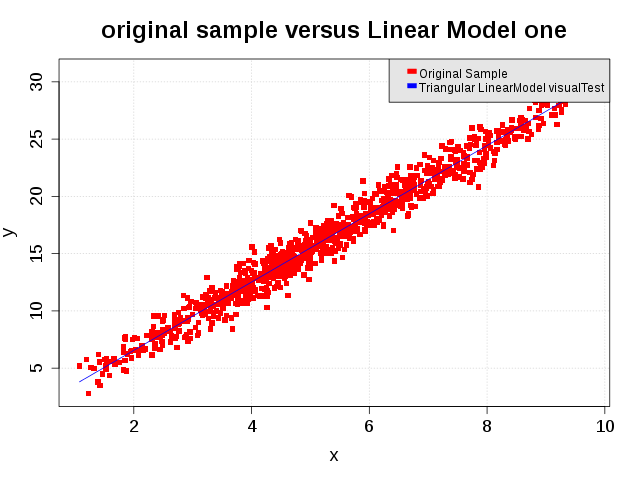
\includegraphics[width=8cm]{Figures/linearRegression_Graph.png}
                       \caption{Visual validation of the Linear Regression Model.}
                       \label{LMGood}
                     \end{center}
                   \end{minipage}
                   \hfill
                   \begin{minipage}{8cm}
                     \begin{center}
                       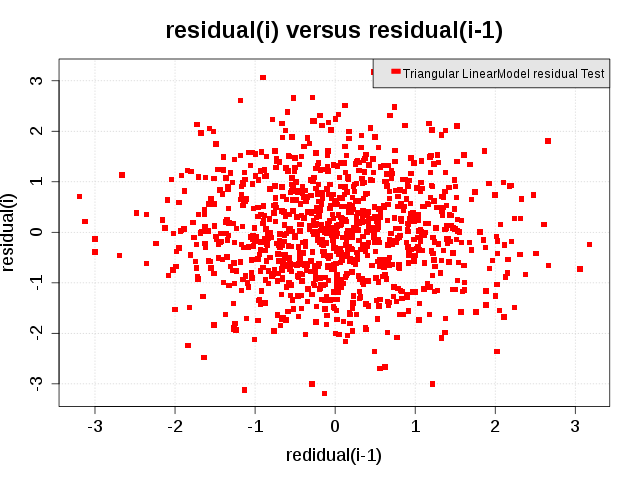
\includegraphics[width=8cm]{Figures/linearRegression_residualGraph.png}
                       \caption{Visual validation of the Linear Regression Model : residuals graph.}
                       \label{LMResidualGood}
                     \end{center}
                   \end{minipage}
                 \end{figure}



                 \begin{figure}[H]
                   \begin{minipage}{8cm}
                     \begin{center}
                       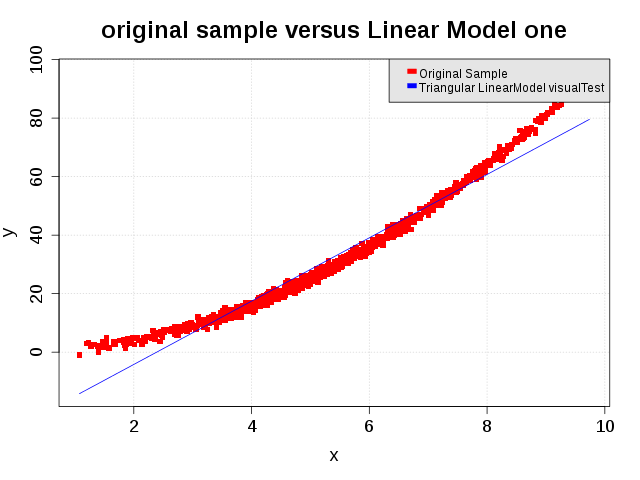
\includegraphics[width=8cm]{Figures/linearRegression_GraphWrong.png}
                       \caption{Visual invalidation of the Linear Regression Model.}
                       \label{LMWrong}
                     \end{center}
                   \end{minipage}
                   \hfill
                   \begin{minipage}{8cm}
                     \begin{center}
                       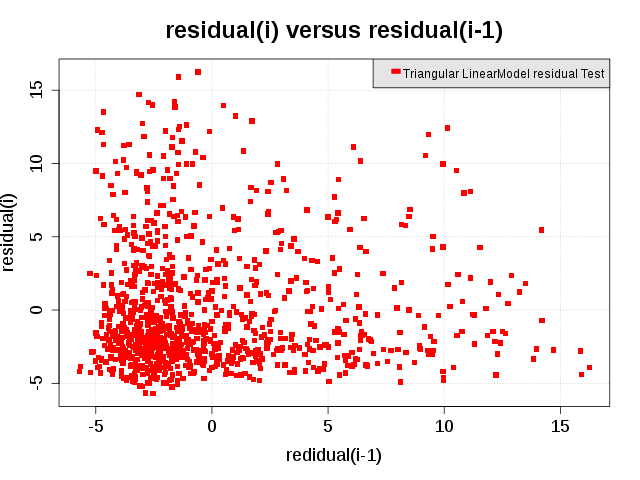
\includegraphics[width=8cm]{Figures/linearRegression_residualGraphWrong.png}
                       \caption{Visual invalidation of the Linear Regression Model : residuals graph.}
                       \label{LMResidualWrong}
                     \end{center}
                   \end{minipage}
                 \end{figure}


                 \begin{figure}[H]
                   \begin{minipage}{8cm}
                     \begin{center}
                       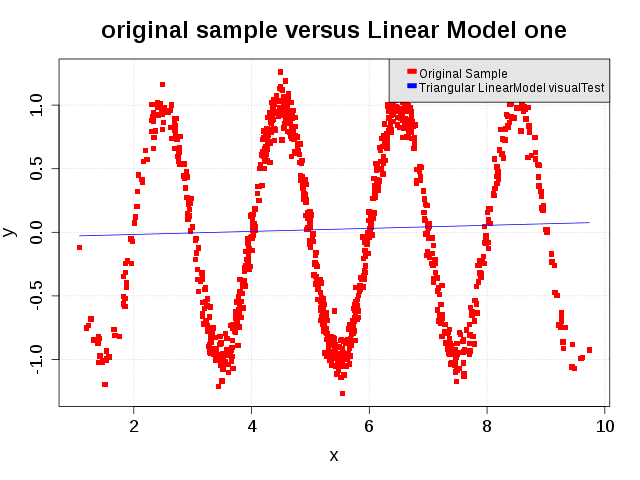
\includegraphics[width=8cm]{Figures/linearRegression_GraphWrong2.png}
                       \caption{Visual invalidation of the Linear Regression Model.}
                       \label{LMWrong2}
                     \end{center}
                   \end{minipage}
                   \hfill
                   \begin{minipage}{8cm}
                     \begin{center}
                       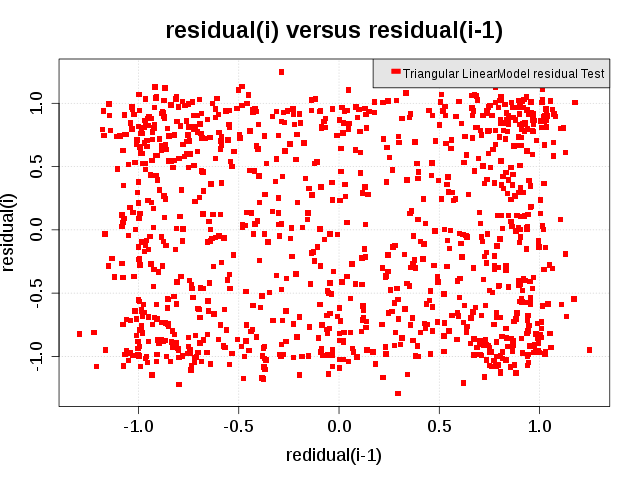
\includegraphics[width=8cm]{Figures/linearRegression_residualGraphWrong2.png}
                       \caption{Visual invalidation of the Linear Regression Model : residuals graph.}
                       \label{LMResidualWrong2}
                     \end{center}
                   \end{minipage}
                 \end{figure}

\newpage % Copyright (C) 2005-2015 Airbus - EDF - IMACS - Phimeca
% Permission is granted to copy, distribute and/or modify this document
% under the terms of the GNU Free Documentation License, Version 1.2
% or any later version published by the Free Software Foundation;
% with no Invariant Sections, no Front-Cover Texts, and no Back-Cover
% Texts.  A copy of the license is included in the section entitled "GNU
% Free Documentation License".
\renewcommand{\filename}{docUC_InputWithData_StatisticalManipulation.tex}
\renewcommand{\filetitle}{UC :  Statistical manipulations on data : min, max, covariance, skewness, kurtosis, quantile, empirical CDF, Pearson, Kendall and Spearman correlation matrixes and rank/sort functionnalities}

% \HeaderNNIILevel
% \HeaderIILevel
\HeaderIIILevel

\label{statistical}


\index{Sample Statistics!Min - Max}
\index{Sample Statistics!Moments evaluation}
\index{Sample Statistics!Covariance}
\index{Sample Statistics!Skewness}
\index{Sample Statistics!Kurtosis}
\index{Sample Statistics!Empirical quantile}
\index{Sample Statistics!Empirical cumulative density function}
\index{Sample Statistics!Pearson correlation coefficient}
\index{Sample Statistics!Kendall's tau}
\index{Sample Statistics!Spearman correlation coefficient}
\index{Sample Statistics! Rank - Sort functionnalities}
\index{Sample Statistics!Cholesky factor}
\index{Quantile!Empirical estimation}



The objective of this Use Case is to describe the main statistical functionalities that OpenTURNS enables to manipulate some data, represented by a NumericalSample.\\





OpenTURNS enables to calculate per components :
\begin{itemize}
\item min and max per component, with the methods {\itshape getMin, getMax}
\item range per component, with the method {\itshape computeRangePerComponent}
\item mean, variance, standard deviation , skewness and kurtosis  per component, with the methods {\itshape computeMean, computeVariancePerComponent, computeStandardDeviationPerComponent, computeSkewnessPerComponent, computeKurtosisPerComponent}
\item empirical median and other quantiles per component, with the methods {\itshape computeMedianPerComponent, computeQuantilePerComponent}
\end{itemize}

OpenTURNS enables some global calculs :
\begin{itemize}
\item covariance of the sample, with the methods {\itshape computeCovariance},
\item standard deviation of the sample : the Cholesky factor of the covariance matrix, with the methods {\itshape computeStandardDeviation },
\item Pearson, Kendall and Spearman correlation matrix, with the methods {\itshape computePearsonCorrelation, computeKendallTau, computeSpearmanCorrelation},
\item empirical CDF evaluated on a point $\vect{x}$ : $\Prob{X_1 \leq x_1, \hdots, X_n \leq x_n}$, with the methods {\itshape computeEmpiricalCDF},
\item empirical tail CDF evaluated on a point $\vect{x}$ : $\Prob{X_1 > x_1, \hdots, X_n > x_n}$, with the methods {\itshape computeEmpiricalCDF},
\item empirical quantiles, with the method {\itshape computeQuantile}. For the quantile $x_q$ of order $q$, OpenTURNS proceeds as follows :
  \begin{itemize}
  \item $\forall q \in [\frac{1}{2n}, 1-\frac{1}{2n}]$, then OpenTURNS approximates the empirical  cumulative density function by interpolating all the middles of the steps and then evaluates  $x_q$ from this continuous approximation.
  \item $\forall q \leq \frac{1}{2n}$, then OpenTURNS returns $min(X_i)$.
  \item $\forall q > \frac{1}{2n}$, then OpenTURNS returns $max(X_i)$.
  \end{itemize}
\end{itemize}

At last, it is possible :
\begin{itemize}
\item to copy into a NumericalSample whose components are the respective ranks of the components, with the method {\itshape rank},
\item to copy into a NumericalSample whose components are all sorted in ascending order, with the method {\itshape sort },
\item to extract the $(i+1)$ component whose components are all sorted in ascending order, with the method {\itshape sort(i) },
\item to copy into a NumericalSample whose NumericalPoints are reordered such that the $(i+1)$ component is sorted in ascending order, with the method  {\itshape sortAccordingAComponent(i)},
\item to keep from the Numericalsample only the $i$ first points, with the method  {\itshape split(i)},
\item to translate the points of the NumericalSample, with the method  {\itshape translate },
\item to multiply all the components of the points by a factor, with the method  {\itshape  scale},
\item to remove a particular point from the NumericalSample, with the method  {\itshape  erase}.
\end{itemize}



\requirements{
  \begin{description}
  \item[$\bullet$] a numerical sample : {\itshape sample}
  \item[type:]  NumericalSample
  \end{description}
}
             {
               \begin{description}
               \item[$\bullet$] statistical elements listed previously
               \item[type:]  NumericalPoint, SquareMatrix or CorrelationMatrix
               \end{description}
             }

             \textspace\\
             Python script for this UseCase :

             \inputscript{script_docUC_InputWithData_StatisticalManipulation}

             \textspace\\



             To illustrate each method, we give here an example in dimension 2 : consider the following NumericalSample \textit{numSample = [(1.3, 1.2); (4.1, 1.0); (2.3, 2.7)]}. Then,

             At last, it is possible :
             \begin{itemize}
             \item \textit{new = numSample.rank()}: \textit{new = [(0,1); (2,0); (1,2)]},
             \item \textit{new = numSample.sort()}: \textit{new = [(1.3,1.0); (2.3,1.2); (4.1,2.7)]},
             \item \textit{new = numSample.sort(0))}: \textit{new = [(1.3); (2.3); (4.1)]},
             \item \textit{new = numSample.sortAccordingAComponent(1)}: \textit{new  = [(4.1, 1.0);(1.3, 1.2);(2.3, 2.7)]},
             \item \textit{new = numSample.split(2)}: \textit{new  = [(2.3, 2.7)]} and \textit{numSample = [(1.3, 1.2); (4.1, 1.0)]},
             \item \textit{new = numSample.translate(NumericalPoint(2,1.0))}: \textit{new  = [(2.3, 2.2); (4.1, 2.0); (3.3, 3.7)]},
             \item \textit{new = numSample.scale(NumericalPoint(2,2.0))}: \textit{new  = [(2.6, 2.4); (8.2, 2.0); (4.6, 5.4)]},
             \item \textit{new = numSample.erase(1)}: \textit{new  = [(1.3, 1.2); (2.3, 2.7)]}.
             \end{itemize}

\newpage % Copyright (C) 2005-2015 Airbus - EDF - IMACS - Phimeca
% Permission is granted to copy, distribute and/or modify this document
% under the terms of the GNU Free Documentation License, Version 1.2
% or any later version published by the Free Software Foundation;
% with no Invariant Sections, no Front-Cover Texts, and no Back-Cover
% Texts.  A copy of the license is included in the section entitled "GNU
% Free Documentation License".
\renewcommand{\filename}{docUC_InputWithData_CloudDrawing.tex}
\renewcommand{\filetitle}{UC :  Draw of clouds}

% \HeaderNNIILevel
% \HeaderIILevel
\HeaderIIILevel



\index{Graph!Clouds of points}
\index{Graph!Pairs graph}
\index{View Image}
\index{Graph!Superposition of graphs}



The objective of this Use Case is to draw a cloud of points when points are bidimensional and all the possible pairs of components when the points are of dimension $n>2$.


\requirements{
  \begin{description}
  \item[$\bullet$] one  sample of dimension 2 : {\itshape sample2d}
  \item[type:]  NumericalSample
  \item[$\bullet$] one  sample of dimension $n=4$ : {\itshape sample4d}
  \item[type:]  NumericalSample
  \end{description}
}
             {
               \begin{description}
               \item[$\bullet$] the files containing the cloud graph
               \item[type:] files in all possible formats
               \end{description}
             }

             \textspace\\
             Python script for this UseCase :

             \inputscript{script_docUC_InputWithData_CloudDrawing}

             \textspace\\



             Figure (\ref{cloud2}) draws the superposition of two clouds of dimension 2 and size 1000, realizations of :
             \begin{itemize}
             \item a Normal distribution with $\vect{0}$ mean, unit standard deviation and independant components,
             \item a Normal distribution with unit-mean,  unit-standard deviation and independant components.
             \end{itemize}

             Figure (\ref{cloud2}) draws all the possible pairs of components from a sample of dimension 4 and size $N=500$, generated by a Normal distribution with correlation matrix $\mat{R} (C_{ij})_{ij}$ such that the components 1 and 2 are correlated with $R_{12} = 0.8$ and the components 3 and 4 are correlated with $R_{34} = -0.7$.

             \begin{figure}[H]
               \begin{center}
                 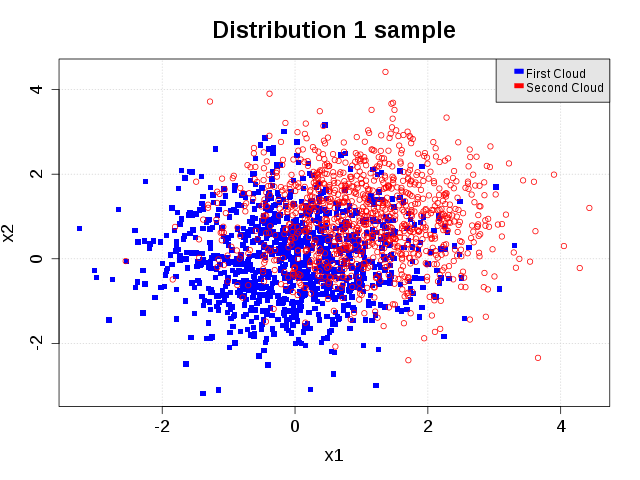
\includegraphics[width=10cm]{Figures/cloud2.png}
               \end{center}
               \caption{Superposition of two normal numerical sample of dimension 2.}
               \label{cloud2}
             \end{figure}


             \begin{figure}[H]
               \begin{center}
                 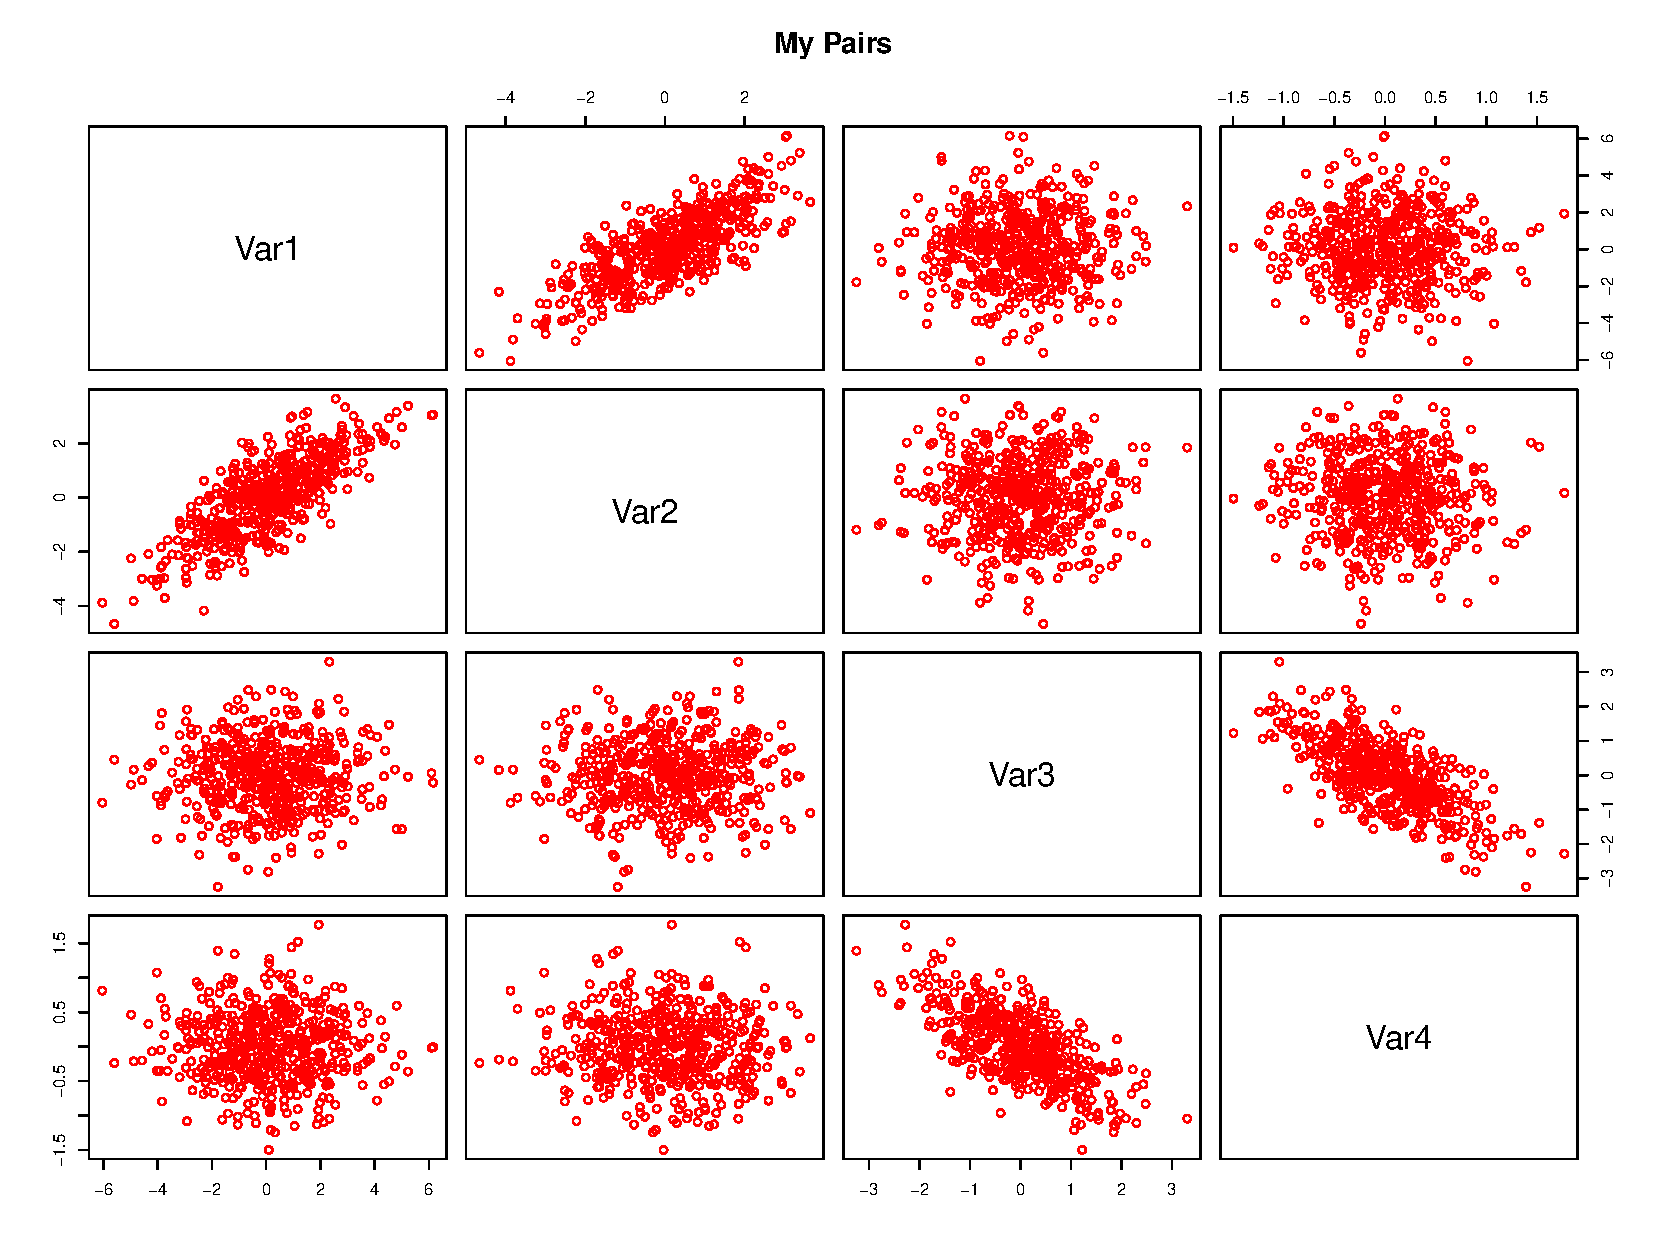
\includegraphics[width=10cm]{Figures/pairs.pdf}
               \end{center}
               \caption{Pairs graph for a sample of dimension 4.}
               \label{cloud2}
             \end{figure}

\newpage % Copyright 2005-2016 Airbus-EDF-IMACS-Phimeca
% Permission is granted to copy, distribute and/or modify this document
% under the terms of the GNU Free Documentation License, Version 1.2
% or any later version published by the Free Software Foundation;
% with no Invariant Sections, no Front-Cover Texts, and no Back-Cover
% Texts.  A copy of the license is included in the section entitled "GNU
% Free Documentation License".
\renewcommand{\filename}{docUC_InputWithData_MaxLikelihood.tex}
\renewcommand{\filetitle}{UC : Maximum likelihood of a given probability density function }

% \HeaderNNIILevel
% \HeaderIILevel
\HeaderIIILevel



\index{Fitting Distribution! Maximum likelihood}


The objective of this Use Case is to explicitate how to implement the evaluation of the parameters of a fitted distribution thanks to the Maximum Likelihood Principle.\\


Details on the Maximum Likelihood  Principle may be found in the Reference Guide (\extref{ReferenceGuide}{see files Reference Guide - Step B -- Maximum Likelihood  Principle}{stepB}).\\

Let us denote $(\vect{x}_1, \dots, \vect{x}_n)$ the sample, $p_{\vect{\theta}}$ the particular distribution of probability density function we want to fit to the sample, and  $\vect{\theta} \in \Theta \in \Rset^p$ its the parameter vector.\\

The likelihood of the sample according to  $p_{\vect{\theta}}$ is :
\begin{align*}
  likelihood(\vect{x}_1, \dots, \vect{x}_n,\vect{\theta}) = \prod_{i=1}^n p_{\vect{\theta}}(\vect{x}_i)
\end{align*}
It may be implemented :
\begin{itemize}
\item either as a python function thanks to the class OpenTURNSPythonFunction, as explained in the UC.\ref{OpenTURNSPythonFunction},
\item or thanks to the NumericalMathFunction class, as explained in the UC.\ref{NumericalMathFunction}.
\end{itemize}

The maximum likelihood estimation $\vect{\theta}_{MLE}$ is solution of the equation :
\begin{align*}
  \max_{\vect{\theta} \in \Theta} likelihood\, (\vect{x}_1, \dots, \vect{x}_n,\vect{\theta})
\end{align*}
or
\begin{align*}
  \max_{\vect{\theta} \in \Theta}  \log likelihood\, (\vect{x}_1, \dots, \vect{x}_n,\vect{\theta})
\end{align*}


The following UC illustrates the example of a Normal distribution, where $(\mu, \sigma) \in \Rset \times \Rset^+$ are defined through the maximum likelihood principle, where the log of the likelihood funciton  is implemented thanks to the OpenTURNSPythonFunction class.\\

Note that to avoid underflow problems with the log of the likelihood function, it is necessary to bound the probability density function to a min value \textit{eps}, here equal to $1.0e-16$. The example illustrates how to proceed.\\


\requirements{
  \begin{description}
  \item[$\bullet$] a sample of data : {\itshape sample}
  \item[type:]  a NumericalSample
  \end{description}
}
             {
               \begin{description}
               \item[$\bullet$] the log likelihood function in the openturns library : {\itshape myLogLikelihoodOT}
               \item[type:] a NumericalMathFunction
               \item[$\bullet$] the  MLE of $(\mu, \sigma)$ : {\itshape optimizer}
               \item[type:] a NumericalPoint
               \end{description}
             }

             \textspace\\
             Python script for this UseCase :

             \inputscript{script_docUC_InputWithData_MaxLikelihood}





%%%%%%%%%%%%%%%%%%%%%%%%%%%%%%
\newpage \subsection{Bayesian modeling}

The objective of this section is to build a random vector or a distribution wich parameters follows a distribution.

% Copyright 2005-2016 Airbus-EDF-IMACS-Phimeca
% Permission is granted to copy, distribute and/or modify this document
% under the terms of the GNU Free Documentation License, Version 1.2
% or any later version published by the Free Software Foundation;
% with no Invariant Sections, no Front-Cover Texts, and no Back-Cover
% Texts.  A copy of the license is included in the section entitled "GNU
% Free Documentation License".
\renewcommand{\filename}{docUC_InputBayesian_CondDist.tex}
\renewcommand{\filetitle}{UC : Creation of a  distribution with uncertain parameters}

% \HeaderNNIILevel
% \HeaderIILevel
\HeaderIIILevel



\index{Distribution!Conditional distribution}
\index{Bayesian! Conditional distribution}

The objective of this Use Case is to create  the distribution of $\vect{X}$ such that $$\vect{X}|\vect{\Theta} \sim \cL_{\vect{X}|\vect{\Theta}}$$ with $$\vect{\Theta}=g(\vect{Y})$$ and $$\vect{Y} \sim \cL_{\vect{Y}}.$$ The function $g$ is a given function of input dimension the dimension of $\cL_{\vect{Y}}$ and output dimension the dimension of $\vect{\Theta}$.\\
We call {\itshape ConditionalDistribution} such a distribution.\\


\requirements{
  \begin{description}
  \item[$\bullet$] distribution of $\vect{X}|\vect{\Theta}$   : {\itshape conditionedDist}
  \item[type:] Distribution
  \item[$\bullet$] distribution of   $\vect{Y}$ : {\itshape conditioningDist}
  \item[type:] Distribution
  \item[$\bullet$] the function $g$ : {\itshape linkFunction}
  \item[type:] NumericalMathFunction
  \end{description}
}
{
  \begin{description}
  \item[$\bullet$] the conditional distribution : {\itshape  finalDist}
  \item[type:]  ConditionalDistribution
  \item[$\bullet$] a sample: {\itshape sampleY}
  \item[type:]  NumericalSample
  \end{description}
}

\textspace\\
Python script for this UseCase :

\inputscript{script_docUC_InputBayesian_CondDist}

\textspace\\

The UC illustrates the distribution of  $X$ that follows a $Uniform(A,B)$ distribution, with $(A,B)=g(Y)$, $g:\Rset \rightarrow \Rset^2, \, g(Y)=(Y, 1+Y^2)$ and $Y$ follows a $Uniform(-1, 1)$ distribution.\\
The figure Fig.\ref{ConditionalPDF} draws the probability density function of $X$.


\begin{figure}[H]
  \begin{center}
    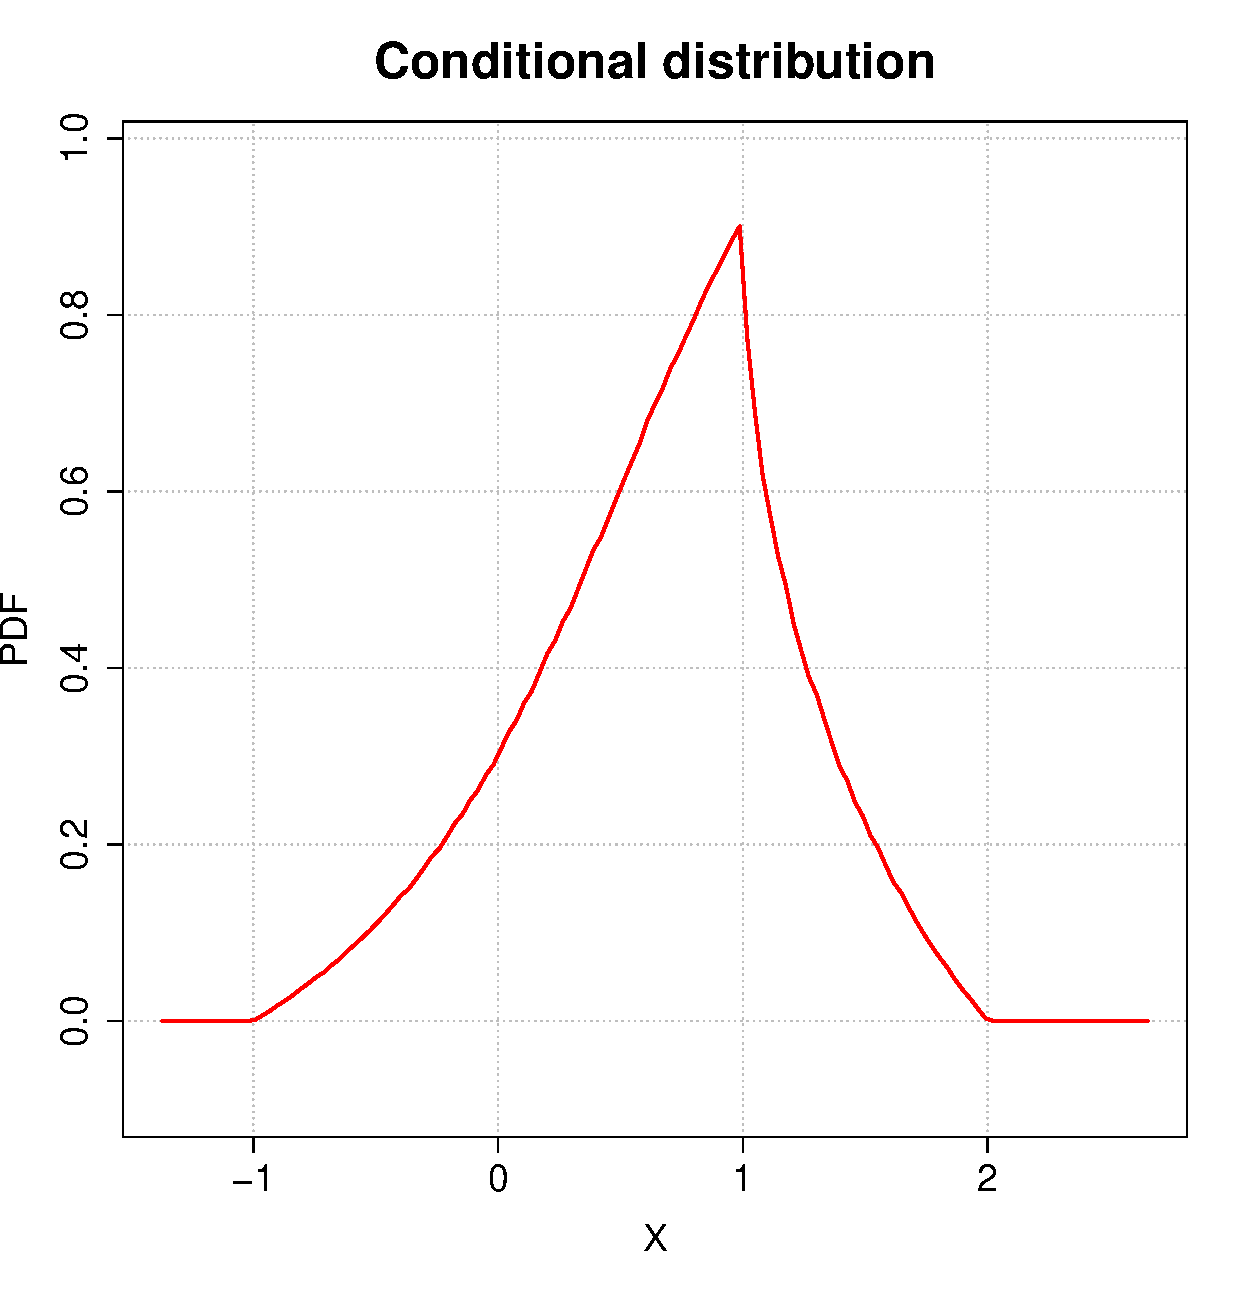
\includegraphics[width=7cm]{Figures/pdf_conditionalDist.pdf}
    \caption{$Uniform(Y, 1+Y^2)$ distribution with $Y\sim Uniform(-1,1)$.}
    \label{ConditionalPDF}
  \end{center}
\end{figure}

%\newpage % Copyright (C) 2005-2015 Airbus - EDF - IMACS - Phimeca
% Permission is granted to copy, distribute and/or modify this document
% under the terms of the GNU Free Documentation License, Version 1.2
% or any later version published by the Free Software Foundation;
% with no Invariant Sections, no Front-Cover Texts, and no Back-Cover
% Texts.  A copy of the license is included in the section entitled "GNU
% Free Documentation License".
\renewcommand{\filename}{docUC_InputBayesian.tex}
\renewcommand{\filetitle}{UC : Creation of a random vector with random parameters}

% \HeaderNNIILevel
% \HeaderIILevel
\HeaderIIILevel



\index{Distribution!Bayesian}
\index{Bayesian! Distribution}

The objective of this Use Case is to create a random vector $\vect{X}$ which distribution $\cL_{\vect{X}|\vect{\Theta}}$ which parameters $\vect{\Theta}$ form a random vector distributed according to the distribution  $\cL_{\vect{\Theta}}$.\\

Note that the random parameters vector $\vect{\Theta}$ is a {\itshape RandomVector} object. We only need its capacity to generate realisations.  It can be :
\begin{itemize}
\item a {\itshape UsualRandomVector} which means described by a given distribution $\cL_{\vect{\Theta}}$;
\item or a {\itshape CompositeRandomVector} which means the output vector of a fonction $f$ evaluated on the random vector $\vect{Y}$  : $\vect{\Theta} = f(\vect{Y})$. In that case, the distribution $\cL_{\vect{\Theta}}$ is a not explicitely known;
\item other complex structures as {\itshape PythonRandomVector, FunctionalChaosRandomVector, Event} \dots.
\end{itemize}

To generate a realization of such a random vector $\vect{X}$, OpenTURNS first generates a realization $\vect{\theta}$  of the random vector  $\vect{\Theta}$ according to  $\cL_{\vect{\Theta}}$, then a realization of the distribution $\cL_{\vect{X}|\vect{\Theta}=\vect{theta}}$.\\


\requirements{
  \begin{description}
  \item[$\bullet$] the distribution $\cL_{\vect{X}|\vect{\Theta}}$: {\itshape myX\_ThetaDist}
  \item[type:] Distribution
  \item[$\bullet$] the distribution $\cL_{\vect{\Theta}}$: {\itshape myThetaDist}
  \item[type:] Distribution
  \item[$\bullet$] the function $f$: {\itshape model}
  \item[type:] NumericalMathFunction
  \item[$\bullet$] the input random vector $\vect{Y}$: {\itshape inputYRV}
  \item[type:] RandomVector
  \end{description}
}
{
  \begin{description}
   \item[$\bullet$] the random vector $\vect{\Theta}$: {\itshape myThetaRV\_1, myThetaRV\_2}
  \item[type:]  RandomVector (of type Usual or Composite)
  \item[$\bullet$] the random vector $\vect{X}$: {\itshape X\_1,X\_2}
  \item[type:]  ConditionalRandomVector
   \item[$\bullet$] the distribution of $\vect{X}$ given $\vect{\Theta}$:  {\itshape Xdist }
  \item[type:] Distribution
  \item[$\bullet$] a random vector: {\itshape rdTheta}
  \item[type:] RandomVector
  \end{description}
}

\textspace\\
Python script for this UseCase :

\inputscript{script_docUC_InputBayesian_RandomVector}

\textspace\\

The following example illustrates a scalar random vector $X$ distributed according to a Normal distribution: $\cL_{\vect{X}|\vect{\Theta}=(M, \Sigma)} = Normal(M, \Sigma)$, wich parameters are defined by:
\begin{itemize}
\item $M \sim Uniform([0,1])$,
\item $\Sigma \sim Exponential(\lambda=4)$.
\end{itemize}

The figure Fig.\ref{DensitCond} draws the probability density function of $X$ that has been built with the kernel smoothing technique from $n=10^6$ realizations of $X$ with the normal kernel. It also draws, for comparison needs, the probability density function of $X$ in the case where the parameters are fixed to their mean value.\\

\begin{figure}[H]
  \begin{center}
    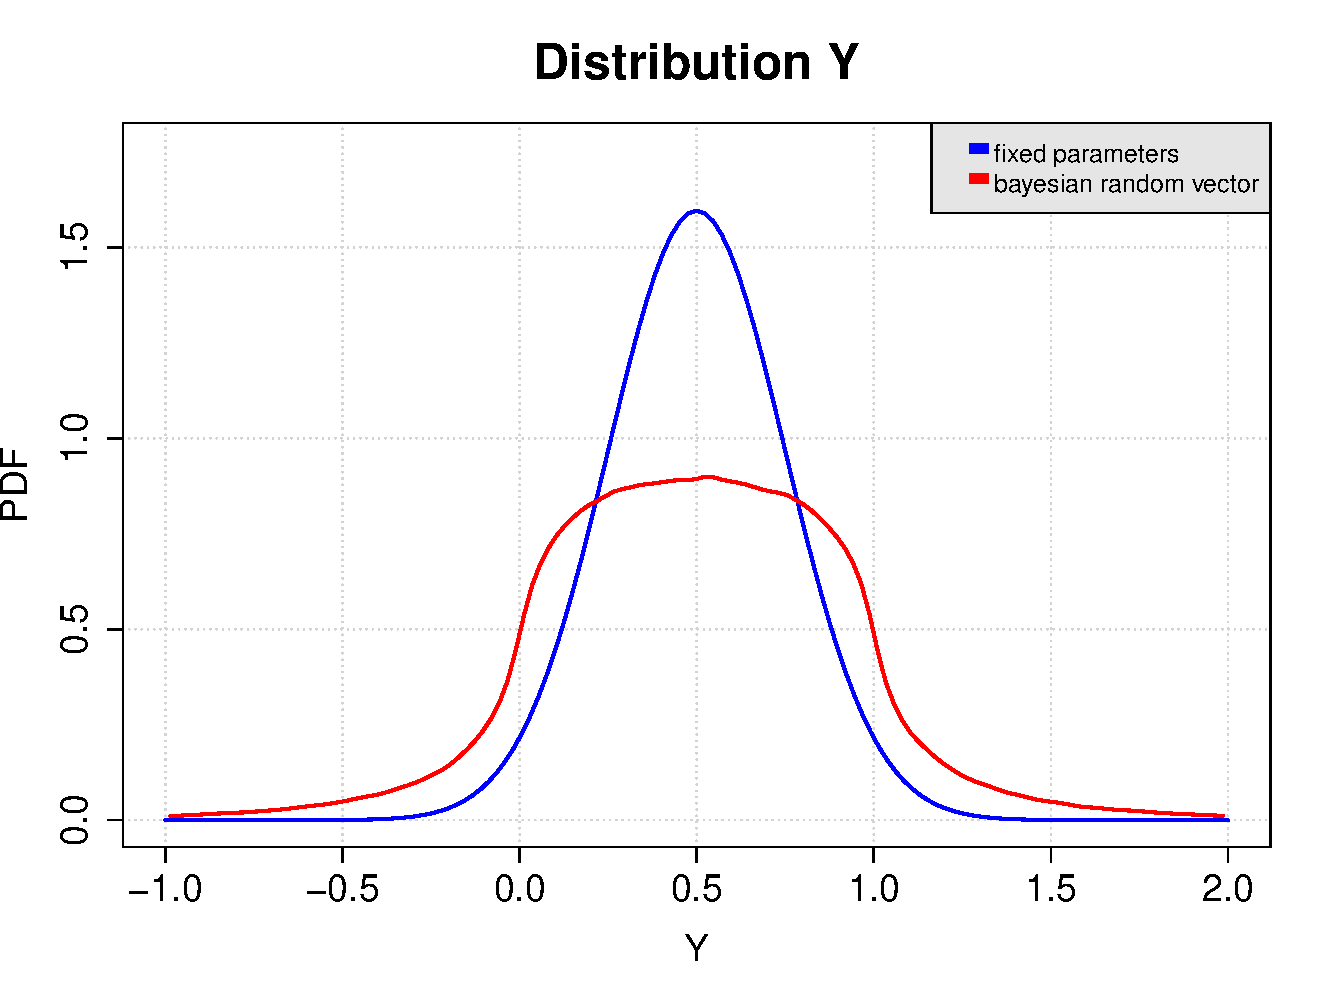
\includegraphics[width=7cm]{Figures/pdf_bayesianRandomVector.pdf}
    \caption{Normal distribution with random or fixed parameters.}
    \label{DensitCond}
  \end{center}
\end{figure}

Besides, if we consider the event $\cE = \{X > 1.5\}$, we have $\Prob{\cE}= 1.75\, e-2$ in the first case of random parameters and $\Prob{\cE}= 3.17\, e-5$ in the case of fixed parameters.\\

Note that we can compare both models using {\itshape ConditionalRandomVector} and {\itshape ConditionalDistribution} objects. We recall that $\vect{X}_{\vect{\Theta}} \sim \cL_{\vect{X}|\vect{\Theta}}$ and $\vect{\Theta} \sim \cL_{\vect{\Theta}}$, where
$\cL_{\vect{X}|\vect{\Theta}}$ and $\cL_{\vect{\Theta}}$ are {\itshape Distribution} objects, $\vect{\Theta}$ is a {\itshape RandomVector} object.\\

Using the {\itshape ConditionalRandomVector} object, we can model $\vect{X}$ as follows:
\begin{align*}\label{CondRV}
  \vect{X} = ConditionalRandomVector(\cL_{\vect{X}|\vect{\Theta}}, \vect{\Theta})
\end{align*}
This model enables to generate realizations of $\vect{X}$ but does not give access to its distribution.\\
According to the way the random vector $\vect{\Theta}$ has been modeled, we can use other equivalent models:
\begin{itemize}
\item $\vect{\Theta}$ is a {\itshape UsualRandomVector}, defined by its {\itshape Distribution} $\cL_{\vect{\Theta}}$:
  \begin{align*}
    \vect{\Theta} = RandomVector(\cL_{\vect{\Theta}})
  \end{align*}
  Then (\ref{CondRV}) is equivalent to:
  \begin{align}\label{CondDist1}
    \vect{X} = RandomVector(ConditionalDistribution(\cL_{\vect{X}|\vect{\Theta}}, \cL_{\vect{\Theta}}))
  \end{align}
  Here we have the fact that by default, the link function is the identity one.

\item $\vect{\Theta}$ is a {\itshape CompositeRandomVector}, defined by $\vect{\Theta} = f(\vect{Y})$, where $\vect{Y}$ is a {\itshape UsualRandomVector},
  defined by its distribution $\cL_{\vect{Y}}$:
  \begin{align*}
    \vect{Y} = & RandomVector(\cL_{\vect{Y}})\\
    \vect{\Theta} = & RandomVector(f, \vect{Y})
  \end{align*}
  Then (\ref{CondRV}) is equivalent to:
  \begin{align}\label{CondDist2}
    \vect{X} = RandomVector(ConditionalDistribution(\cL_{\vect{X}|\vect{\Theta}}, \cL_{\vect{Y}}, f))
  \end{align}
  If $\vect{\Theta}$ and $\vect{Y}$ are of dimension 1, then we can use the {\itshape CompositeDistribution} object to define the distribution $\cL_{\vect{\Theta}}$ as follows:
  \begin{align}\label{CondDist3}
    \vect{X} = RandomVector(ConditionalDistribution(\cL_{\vect{X}|\vect{\Theta}}, CompositeDistribution(f,\cL_{Y}))
  \end{align}

\end{itemize}
Note that all the modellings (\ref{CondDist1}), (\ref{CondDist2}) and (\ref{CondDist3}) give access to the final distribution of $\vect{X}$ and thus enable to use all the methods inherent to a {\itshape Distribution} object, such as {\itshape computeMean(), \dots}.
\newpage % Copyright 2005-2016 Airbus-EDF-IMACS-Phimeca
% Permission is granted to copy, distribute and/or modify this document
% under the terms of the GNU Free Documentation License, Version 1.2
% or any later version published by the Free Software Foundation;
% with no Invariant Sections, no Front-Cover Texts, and no Back-Cover
% Texts.  A copy of the license is included in the section entitled "GNU
% Free Documentation License".
\renewcommand{\filename}{docUC_InputBayesian_BayesDist.tex}
\renewcommand{\filetitle}{UC : Creation of a multivariate distribution through conditioning}

% \HeaderNNIILevel
% \HeaderIILevel
\HeaderIIILevel



\index{Distribution!Bayesian}
\index{Bayesian! Distribution}

The objective of this Use Case is to create  the distribution of the random vector $(\vect{X},\vect{Y})$ where $$\vect{Y} \sim \cL_{\vect{Y}}$$ and $$\vect{X}|\vect{\Theta} \sim \cL_{\vect{X}|\vect{\Theta}}$$  whith $$\vect{\Theta}=g(\vect{Y})$$ where $g$ a given function of input dimension the dimension of $\cL_{\vect{Y}}$ and output dimension the dimension of $\vect{\Theta}$.


\requirements{
  \begin{description}
  \item[$\bullet$] distribution of $\vect{X}|\vect{\Theta}$   : {\itshape conditionedDist}
  \item[type:] Distribution
  \item[$\bullet$] distribution of   $\vect{Y}$ : {\itshape conditioningDist}
  \item[type:] Distribution
  \item[$\bullet$] the function $g$ : {\itshape linkFunction}
  \item[type:] NumericalMathFunction
  \end{description}
}
{
  \begin{description}
  \item[$\bullet$] the conditional distribution : {\itshape  finalDist}
  \item[type:]  ConditionalDistribution
  \item[$\bullet$] a sample: {\itshape sampleY}
  \item[type:]  NumericalSample
  \end{description}
}

\textspace\\
Python script for this UseCase :

\inputscript{script_docUC_InputBayesian_BayesDist}

\textspace\\

The UC illustrates the distribution of  $X$ that follows a $Uniform(A,B)$ distribution, with $(A,B)=(Y, 1+Y)$ where $Y$ follows a $Uniform(-1, 1)$ distribution.\\
The figure Fig.\ref{BayesPDF} draws a sample of $(X, Y)$.


\begin{figure}[H]
  \begin{center}
    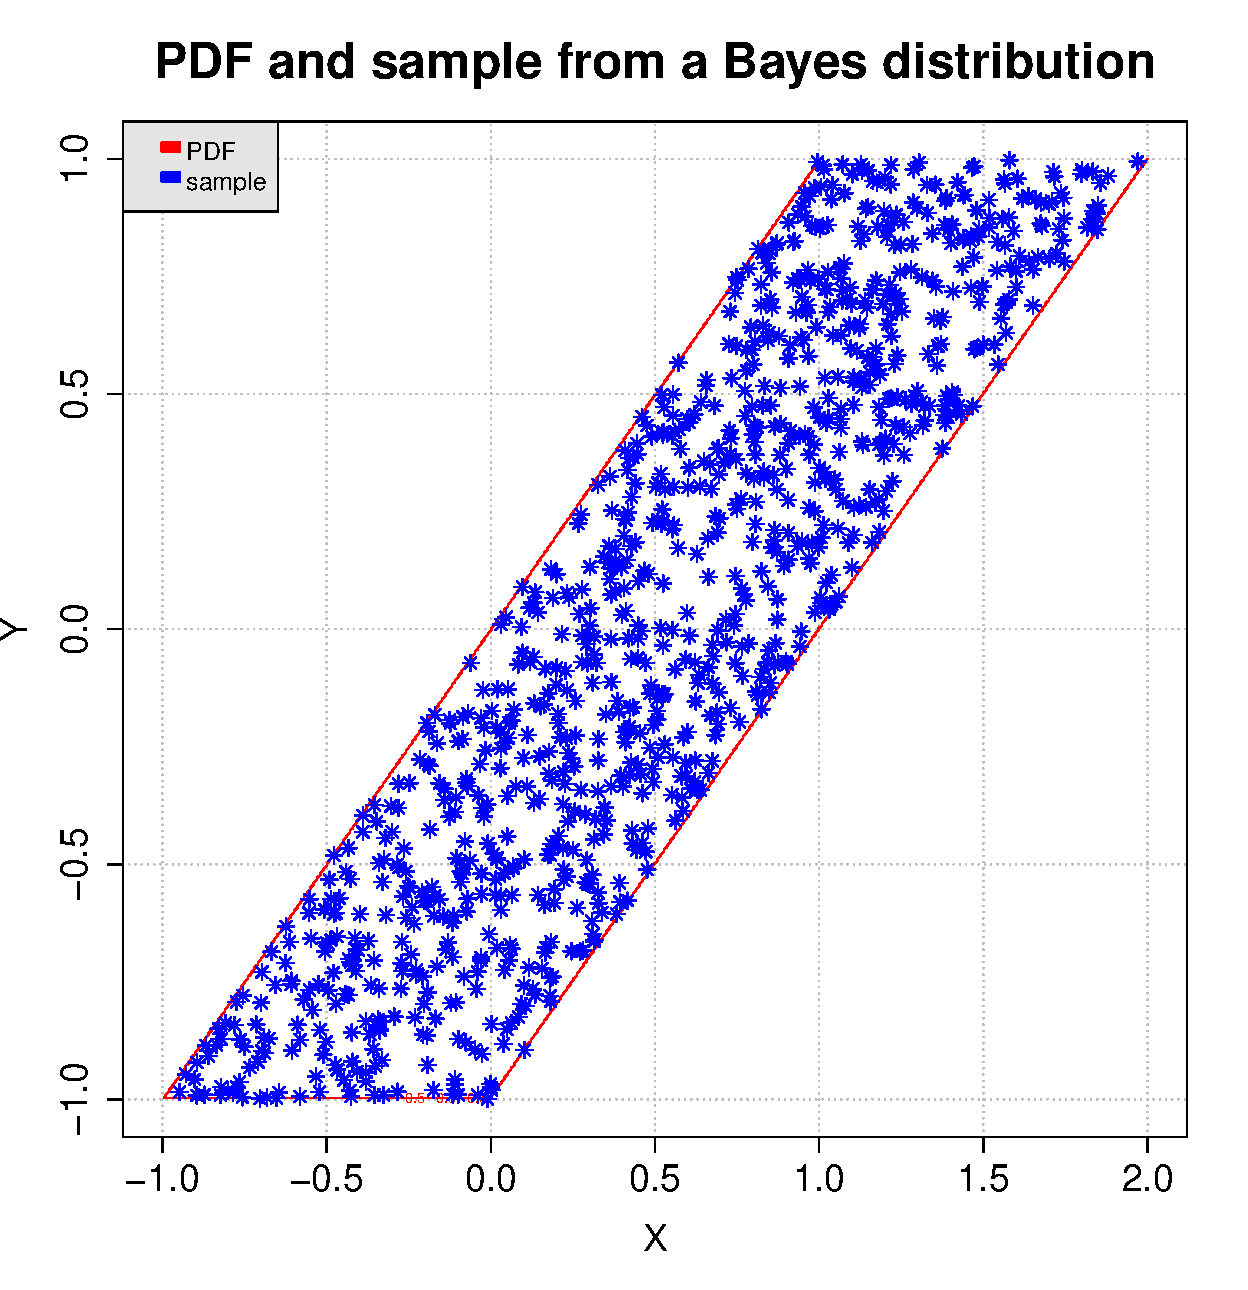
\includegraphics[width=7cm]{Figures/pdf_bayesianDist.pdf}
    \caption{Iso-PDF and sample of $(X, Y)$ where $X \sim Uniform(Y, 1+Y)$ and $Y \sim Uniform(-1,1)$.}
    \label{BayesPDF}
  \end{center}
\end{figure}

\newpage % Copyright 2005-2016 Airbus-EDF-IMACS-Phimeca
% Permission is granted to copy, distribute and/or modify this document
% under the terms of the GNU Free Documentation License, Version 1.2
% or any later version published by the Free Software Foundation;
% with no Invariant Sections, no Front-Cover Texts, and no Back-Cover
% Texts.  A copy of the license is included in the section entitled "GNU
% Free Documentation License".
\renewcommand{\filename}{docUC_InputWithData_BayesianCalibration.tex}
\renewcommand{\filetitle}{UC : Bayesian Calibration of a Computer Code}

% \HeaderNNIILevel
% \HeaderIILevel
\HeaderIIILevel



% \index{Fitting Distribution! Maximum likelihood}


The objective of this Use Case is to explicitate how to implement the evaluation of the parameters of a computer model thanks to Bayesian estimation.\\


Details on the Principle of Bayesian Calibration may be found in the Reference Guide (\extref{ReferenceGuide}{see files Reference Guide - Step B -- Bayesian Calibration}{stepB}).\\

Let us denote $\vect y = (y_1, \dots, y_n)$ the observation sample, $\vect z = (f(x_1|\vect{\theta}), \ldots, f(x_n|\vect{\theta}))$ the model prediction, $p(y |z)$ the density function of observation $y$ conditional on model prediction $z$, and $\vect{\theta} \in \Rset^p$ the calibration parameters we wish to estimate.\\

The following objects need to be defined in order to perform Bayesian calibration with Open-TURNS:

\begin{itemize}
\item the conditional density $p(y|z)$ must be defined as a probability distribution, as explained in the UC.% je ne sais comment trouver la reference pour le UC Usual Distributions
\item The computer model must be implemented thanks to the NumericalMathFunction class, as explained in the section \ref{sec:LSFcreation}. This takes a value of $\vect{\theta}$ as input, and outputs the vector of model predictions $\vect z$, as defined above (the vector of covariates $\vect x = (x_1, \ldots, x_n)$ is treated as a known constant). When doing that, we have to keep in mind that $z$ will be used as the vector of parameters corresponding to the distribution specified for $p(y |z)$. For instance, if $p(y|z)$ is normal, this means that $z$ must be a vector containing the mean and variance of $y$ (see the example below)
\item the prior density $\pi(\vect{\theta})$ encoding the set of possible values for the calibration parameters, each value being weighted by its {\em a priori} proabibility, reflecting the beliefs about the possible values of $\vect{\theta}$ before consideration of the experimental data. Again, this is implemented as a probability distribution
\item The Metropolis-Hastings algorithm that samples from the posterior distribution of the calibration parameters requires a vector $\vect{\theta}_0$ initial values for the calibration parameters, as well as the proposal laws used to update each parameter sequentially.
\end{itemize}

The posterior distribution is given by Bayes' theorem :
\begin{align*}
  \pi(\vect{\theta} | \vect y)
  \quad \substack{~\\[0.5em]\displaystyle\propto\\\scriptstyle\vect{\theta}} \quad
  L\left(\vect y | \vect{\theta}\right) \times \pi(\vect{\theta})
\end{align*}
(where $\substack{~\\[0.5em]\displaystyle\propto\\\scriptstyle\vect{\theta}}$
means "proportional to", regarded as a function of $\vect{\theta}$)
and is approximated here by the empirical distribution of the sample $\vect{\theta}^1, \ldots, \vect{\theta}^N$ generated by the Metropolis-Hastings algorithm. This means that any quantity characteristic of the posterior distribution (mean, variance, quantile, \ldots) is approximated by its empirical counterpart.

The following UC illustrates the example of a standard normal linear regression, where
\begin{align*}
  y_i = \theta_1 + x_i \theta_2 + x_i^2 \theta_3 + \varepsilon_i,
\end{align*}
where $\varepsilon_i \stackrel{i.i.d.}{\sim} \mathcal N(0, 1)$
and we use a normal prior on $\vect{\theta}$:
\begin{align*}
  \pi(\vect{\theta}) = \mathcal N(0 ; 100 I_3).
\end{align*}

The UC is divided into two Python scripts:
\begin{itemize}
\item the first one shows how to define the requirements of the second
  according to the normal linear regression example above (it provides
  some data);
\item the second illustrates how carrying out a Bayesian calibration
  in a general context using the RandomWalkMetropolisHastings class.
\end{itemize}

First Python script for this UseCase:

\inputscript{script_docUC_InputWithData_BayesianCalibration1}

\newpage

Second Python script for this UseCase :

\requirements{
  \begin{description}
  \item[$\bullet$] a prior distribution: {\itshape prior}
  \item[type:]  a Distribution
  \item[$\bullet$] a conditional distribution: {\itshape conditional}
  \item[type:]  a Distribution
  \item[$\bullet$] a model: {\itshape model}
  \item[type:]  a NumericalMathFunction
  \item[$\bullet$] a sample of data: {\itshape y\_obs}
  \item[type:]  a NumericalSample
  \end{description}
}
             {
               \begin{description}
               \item[$\bullet$] a Random Walk Metropolis-Hastings (RWMH) sampler: {\itshape RWMHsampler}
               \item[type:] a RandomWalkMetropolisHastings
               \item[$\bullet$] a posterior random vector: {\itshape myRandomVector}
               \item[type:] a PosteriorRandomVector
               \end{description}
             }

             \inputscript{script_docUC_InputWithData_BayesianCalibration2}



%%%%%%%%%%%%%%%%%%%%%%%%%%%%%%%%%%%%%%%%%%%%%%%%%%%%%%%%%%%%%%%%%%%%%%%%%%%%%%%%%%%%%%%%%%
\newpage \section{Creation of the limit state function and the output variable of interest}


The objective of the section is to specify the limit state function and the output variable of interest, defined from the limit state function.\\
It corresponds to the step 'Step A : Specify the output variable of interest' of the global methodology
(\extref{ReferenceGuide}{see Reference Guide - Global Methodology for an uncertainty study - Part A : specification of the case-study}{stepA}).


%%%%%%%%%%%%%%%%%%%%%%%%%%%%%%
\subsection{Creation of the limit state function}
\label{sec:LSFcreation}

% Copyright 2005-2016 Airbus-EDF-IMACS-Phimeca
% Permission is granted to copy, distribute and/or modify this document
% under the terms of the GNU Free Documentation License, Version 1.2
% or any later version published by the Free Software Foundation;
% with no Invariant Sections, no Front-Cover Texts, and no Back-Cover
% Texts.  A copy of the license is included in the section entitled "GNU
% Free Documentation License".
\renewcommand{\filename}{docUC_LSF_Analytical.tex}
\renewcommand{\filetitle}{UC : From an analytical formula declared inline}

% \HeaderNNIILevel
% \HeaderIILevel
\HeaderIIILevel


\index{Limit State Function!Analytical formula declared in line}
\index{Limit State Function!Gradient}
\index{Limit State Function!Hessian}


The objective of this Use Case is to specify the limit state function, defined through an analytical formula declared in line.\\

OpenTURNS automatically evaluates the analytical expressions of the gradient and the hessian, except if the analytical expression of the function is not differentiable everywhere. In that case, OpenTURNS implements a finite difference method :
\begin{itemize}
\item the gradient evaluation method is the centered finite difference method, with the differential increment $h=1e-5$ for each direction,
\item the hessian evaluation method is the centered finite difference method, with the differential increment $h=1e-4$ for each direction.
\end{itemize}




The example here is the analytical function {\itshape myAnalyticalFunction} defined by the formula :
\begin{align*}
  \begin{array}{l|cll}
    myAnalyticalFunction : &   \Rset^2 & \rightarrow & \Rset \\
    & (x_0, x_1)     & \mapsto     & y_0 = -(6+x_0^2-x_1)
  \end{array}
\end{align*}

In the case of functions $scalarF : \Rset  \rightarrow \Rset$, a simplified constructor exists that requires to define the description of the scalar input and the description of the formulas. We give the example where $scalarF(x) = x^2$.\\

\textspace\\

\requirements{
  \begin{description}
  \item[$\bullet$] none
  \end{description}
}
             {
               \begin{description}
               \item[$\bullet$] some functions : {\itshape myAnalyticalFunction, scalarF}
               \item[type:] NumericalMathFunction
               \end{description}
             }

             \textspace\\
             Python script for this Use Case :

             \inputscript{script_docUC_LSF_Analytical}

\newpage % Copyright 2005-2016 Airbus-EDF-IMACS-Phimeca
% Permission is granted to copy, distribute and/or modify this document
% under the terms of the GNU Free Documentation License, Version 1.2
% or any later version published by the Free Software Foundation;
% with no Invariant Sections, no Front-Cover Texts, and no Back-Cover
% Texts.  A copy of the license is included in the section entitled "GNU
% Free Documentation License".
\renewcommand{\filename}{docUCLSF_PythonScript.tex}
\renewcommand{\filetitle}{UC : From a fonction defined in the script python}

% \HeaderNNIILevel
% \HeaderIILevel
\HeaderIIILevel

\label{OpenTURNSPythonFunction}

\index{Limit State Function!Function declarde in the script python}


The objective of this Use Case is to create the limit state function, from a function defined in the script python. OpenTURNS automatically gives to the analytical formula an implementation for the gradient and the hessian : by default,
\begin{itemize}
\item the gradient evaluation method is the  centered finite difference method, with the differential increment $h=1e-5$ for each direction,
\item the hessian evaluation method is the  centered finite difference method, with the differential increment $h=1e-4$ for each direction.
\end{itemize}
It is possible to change the evaluation method for the gradient or the hessian. The following Use Case shows how to proceed.\\




In order to be able to use the function with the {\itshape openturns} library, it is necessary to define a class which derives from {\itshape OpenTURNSPythonFunction} as indicated belows. The example here is the functions {\itshape modelePYTHON} and {\itshape modelePYTHON2}:
\begin{equation}
  \begin{array}{l|lcl}
    modelePYTHON : & \Rset^4 & \rightarrow & \Rset \\
    & (E,F,L,I)    & \mapsto     & \displaystyle \frac{FL^3}{3EI}
  \end{array}
\end{equation}

\begin{equation}
  \begin{array}{l|lcl}
    modelePYTHON2 : & \Rset^4 & \rightarrow & \Rset^2 \\
    & (a,b,c)    & \mapsto     & \displaystyle (a^2, abc)
  \end{array}
\end{equation}


\requirements{
  \begin{description}
  \item[$\bullet$] none
  \end{description}
}
             {
               \begin{description}
               \item[$\bullet$] the python function assoiated to the model: {\itshape modelePYTHON}
               \item[type:] a OpenTURNSPythonFunction
               \item[$\bullet$] the limit state function : {\itshape modeleOpenTURNS}
               \item[type:] a NumericalMathFunction
               \end{description}
             }

             \textspace\\
             Python script for this Use Case :
             \inputscript{script_docUC_LSF_PythonScript}

\newpage % Copyright (C) 2005-2015 Airbus - EDF - IMACS - Phimeca
% Permission is granted to copy, distribute and/or modify this document
% under the terms of the GNU Free Documentation License, Version 1.2
% or any later version published by the Free Software Foundation;
% with no Invariant Sections, no Front-Cover Texts, and no Back-Cover
% Texts.  A copy of the license is included in the section entitled "GNU
% Free Documentation License".
\renewcommand{\filename}{docUC_LSF_SomeParticularFunctions.tex}
\renewcommand{\filetitle}{UC : Some particular functions : linear combination, agregation, composition}

% \HeaderNNIILevel
% \HeaderIILevel
\HeaderIIILevel


\label{NumericalMathFunction}






\index{Limit State Function!Composition}
\index{Limit State Function!Linear combination}
\index{Limit State Function!Agregated funtion}
\index{Limit State Function!Gradient}
\index{Limit State Function!Hessian}

The objective of this Use Case is to create some particular functions :
\begin{itemize}
\item the scalar linear combination \textit{linComb} of vectorial functions $vectFctColl = (f_1, \hdots, f_N)$ where
  \begin{align*}
    \forall 1 \leq i \leq N, \,     f_i : \Rset^n \longrightarrow \Rset^{p}
  \end{align*}
  with specific scalar weights $scalWeight = (c_1, \hdots, c_N)\in \Rset^N $ :
  \begin{align*}
    \begin{array}{l|lcl}
      linComb : & \Rset^n & \longrightarrow & \Rset^{p} \\
      &  \vect{X} & \longrightarrow & \displaystyle \sum_{i=1}^N c_if_i (\vect{X})
    \end{array}
  \end{align*}


\item the vectorial linear combination \textit{vectLinComb} of a set of  functions $scalFctColl = (f_1, \hdots, f_N)$ where
  \begin{align*}
    \forall 1 \leq i \leq N, \,     f_i : \Rset^n \longrightarrow \Rset
  \end{align*}
  with specific vectorial weights $vectWeight = (\vect {c}_1, \hdots, \vect{c}_N)$  where
  \begin{align*}
    \forall 1 \leq i \leq N, \,   \vect{c}_i \in \Rset^p
  \end{align*}
  \begin{align*}
    \begin{array}{l|lcl}
      vectLinComb : & \Rset^n & \longrightarrow & \Rset^{p} \\
      &  \vect{X} & \longrightarrow & \displaystyle \sum_{i=1}^N \vect{c}_if_i (\vect{X})
    \end{array}
  \end{align*}

\item the agregated function $h$ of a set of functions $(f_1, \hdots, f_N)$ where
  \begin{align*}
    f_i : \Rset^n \longrightarrow \Rset^{p_i}
  \end{align*}
  \begin{align*}
    \begin{array}{l|lcl}
      agregFct : & \Rset^n & \longrightarrow & \Rset^{p} \\
      &  \vect{X} & \longrightarrow & (f_1(\vect{X}), \hdots, f_N(\vect{X}))^t
    \end{array}
  \end{align*}
  with
  \begin{align*}
    p = \displaystyle \sum_{i=1}^N p_i
  \end{align*}

\item the indicator function $l$ of an event defined by a function $f$, a comparison operator and a threshold $s$. For example, if the comparison operator is $>$, then
  \begin{align*}
    l = 1_{\{f > s\}}
  \end{align*}
\end{itemize}


OpenTURNS automatically evaluates the analytical expressions of the gradient and the hessian, except if the analytical expression of the function is not differentiable everywhere. In that case, OpenTURNS implements a finite difference method :
\begin{itemize}
\item the gradient evaluation method is the centered finite difference method, with the differential increment $h=1e-5$ for each direction,
\item the hessian evaluation method is the centered finite difference method, with the differential increment $h=1e-4$ for each direction.
\end{itemize}

\requirements{
  \begin{description}
  \item[$\bullet$] some collections of scalar and vectorial functions : {\itshape scalFctColl, vectFctColl}
  \item[type:] some NumericalMathFunctionCollection
  \item[$\bullet$] a list of  scalar weights : {\itshape scalWeight}
  \item[type:] a NumericalPoint
  \item[$\bullet$] a list of  vectorial weights : {\itshape vectWeight}
  \item[type:] a NumericalSample
  \item[$\bullet$] a function : {\itshape function}
  \item[type:] a NumericalMathFunction
  \end{description}
}
             {
               \begin{description}
               \item[$\bullet$] some particular funtions : {\itshape linComb, vectLinComb, agregFct, indFactor}
               \item[type:] some NumericalMathFunction
               \end{description}
             }

             \textspace\\
             Python script for this UseCase :

             \inputscript{script_docUC_LSF_SomeParticularFunctions}

\newpage % Copyright 2005-2016 Airbus-EDF-IMACS-Phimeca
% Permission is granted to copy, distribute and/or modify this document
% under the terms of the GNU Free Documentation License, Version 1.2
% or any later version published by the Free Software Foundation;
% with no Invariant Sections, no Front-Cover Texts, and no Back-Cover
% Texts.  A copy of the license is included in the section entitled "GNU
% Free Documentation License".
\renewcommand{\filename}{docUC_LSF_DeterministicVar2.tex}
\renewcommand{\filetitle}{UC : Introducing some deterministic variables, optimizing memory and CPU time}

% \HeaderNNIILevel
% \HeaderIILevel
\HeaderIIILevel



\index{Limit State Function!Reducing the initial limit state function}
\index{Random Vector!Output random vector}

The objective of this Use Case is to restrict a model which has been previously declared, to some of its variables, through an optimized way.\\

Let's have the same context than in the UC\ref{linearNumericalMathFunction}. The idea here is to avoid the introduction of the potentially huge matrix $\mat{A}$ and the gradient matrix and hessian tensor  of the functions \textit{increase} and \textit{poutre}. For that last problem, it is sufficient to define the gradient matrix and hessian tensor to the final function \textit{poutreReduced} from a finite difference technique.\\

The function {\itshape increase} is defined as follows :
\begin{align*}
  \begin{array}{l|lcl}
    increase : & \Rset^{n_{prob}}  & \rightarrow & \Rset^n \\
    &  \vect{X}_{prob} =
    \begin{array}{|l}
      "inputProb1" \\
      \cdots       \\
      "inputProbNprob"
    \end{array}
    & \mapsto     & increase(\vect{X}_{prob}) =
    \begin{array}{|l}
      "inputProb1" \\
      \cdots       \\
      "inputProbNprob" \\
      valDet1 \\
      \cdots       \\
      valDetNdet
    \end{array}
  \end{array}
\end{align*}

where all the $(valDet1, ..., valDetNdet)$ are the $n_{det}$ values of the determinist components of $\vect{X}$.\\

The same example is re-written in the folloing Use Case.

\requirements{
  \begin{description}
  \item[$\bullet$] the initial limit state function : {\itshape poutre}
  \item[type:] LinearNumericalMathFunction $(\Rset^4 \rightarrow \Rset)$
  \end{description}
}
{
  \begin{description}
  \item[$\bullet$] the {\itshape increase} function
  \item[type:] NumericalMathFunction $(\Rset^2 \rightarrow \Rset^4)$
  \item[$\bullet$]  the new limit state function : {\itshape poutreReduced = poutre $\circ$ increase}
  \item[type:] NumericalMathFunction $(\Rset^2 \rightarrow \Rset)$
  \end{description}
}

\textspace\\
Python script for this UseCase :

\inputscript{script_docUC_LSF_DeterministicVar2}

\newpage % Copyright (C) 2005-2015 Airbus - EDF - IMACS - Phimeca
% Permission is granted to copy, distribute and/or modify this document
% under the terms of the GNU Free Documentation License, Version 1.2
% or any later version published by the Free Software Foundation;
% with no Invariant Sections, no Front-Cover Texts, and no Back-Cover
% Texts.  A copy of the license is included in the section entitled "GNU
% Free Documentation License".
\renewcommand{\filename}{docUC_LSF_ExpertMixture.tex}
\renewcommand{\filetitle}{UC : Defining a piece wise function according to a classifier}

% \HeaderNNIILevel
% \HeaderIILevel
\HeaderIIILevel


\label{ExpertMixture}

\index{Limit State Function!ExpertMixture}


The objective of this Use Case is define a piece wise function according to a classifier:
\begin{eqnarray}\label{expMixtFct}
  f(\vect{x})  & = f_1(\vect{x}) \quad \forall \vect{x} \in Classe\, 1 \\ \nonumber
  & = f_k(\vect{x}) \quad \forall \vect{x} \in Classe\, k  \\\nonumber
  & = f_N(\vect{x}) \quad \forall \vect{x} \in Classe\, N
\end{eqnarray}
where the $N$ classes are defined by the  classifier.



The classifier is MixtureClassifier based on a  MixtureDistribution defined as:
\begin{equation}\label{MixtDist}
  p(\vect{x}) = \sum_{i=1}^N w_ip_i(\vect{x})
\end{equation}

The rule to assign a point to a class is defined as follows:  $\vect{x}$ is assigned to the class $i=\argmax_k \log w_kp_k(\vect{x})$.\\
The grade of $\vect{x}$ with respect to the classe $k$ is $\log w_kp_k(\vect{x})$.\\

The example here is a bivariate classifier that classes points among 2 classes, using the mixture distribution defined by:
\begin{equation}\label{MixtDist}
  p(\vect{x}) = \frac{1}{2}(\phi_1(\vect{x}) + \phi_2(\vect{x}))
\end{equation}
with $\phi_i$ the probability density function of the $Normal(\vect{\mu}, \vect{\sigma}, \mat{R}_i)$ where $\vect{\mu}=(-1, 1)^t$, $\vect{\sigma}=(1, 1)^t$, $\mat{R}_1[0,1]=-0.99$ and $\mat{R}_2[0,1]=0.99$.
The  function $f$ is defined by:
\begin{eqnarray}\label{expMixtFctEx}
  f(\vect{x})  & = -\vect{x} \quad \forall \vect{x} \in Classe\, 1 \\ \nonumber
  & = +\vect{x} \quad \forall \vect{x} \in Classe\, 2
\end{eqnarray}

\requirements{-
}
             {
               \begin{description}
               \item[$\bullet$] the {\itshape moe}: model of expert mixture
               \item[type:] ExpertMixture
               \end{description}
             }

             \textspace\\
             Python script for this Use Case :

             \inputscript{script_docUC_LSF_ExpertMixture}

\newpage % Copyright (C) 2005-2015 Airbus - EDF - IMACS - Phimeca
% Permission is granted to copy, distribute and/or modify this document
% under the terms of the GNU Free Documentation License, Version 1.2
% or any later version published by the Free Software Foundation;
% with no Invariant Sections, no Front-Cover Texts, and no Back-Cover
% Texts.  A copy of the license is included in the section entitled "GNU
% Free Documentation License".
\renewcommand{\filename}{docUC_LSF_NMFManipulation.tex}
\renewcommand{\filetitle}{UC : Manipulation of a NumericalMathFunction}

% \HeaderNNIILevel
% \HeaderIILevel
\HeaderIIILevel



\index{Numerical Math Function Manipulation!Dimension}
\index{Numerical Math Function Manipulation!Gradient}
\index{Numerical Math Function Manipulation!Hessian}
\index{Numerical Math Function Manipulation!Marginal}
\index{Numerical Math Function Manipulation!Evaluation}
\index{Numerical Math Function Manipulation!Composition}
\index{Numerical Math Function Manipulation!History}
\index{Numerical Math Function Manipulation!Graph}


The objective of this Use Case  is to describe the main functionalities of OpenTURNS  to manipulate a numerical function $f : \Rset^n  \longrightarrow \Rset^p$.\\

OpenTURNS enables :
\begin{itemize}
\item to ask the dimension of its input and output vectors, with the methods {\itshape getInputDimension,  getOutputDimension},
\item to evaluate itself, its gradient and hessian, with the methods {\itshape gradient, hessian}. The evaluation of the function is a vector of dimension $p$, the gradient is a matrix with $p$ rows and $n$ columns, the hessian is a tensor of order 3 with  $p$ rows, $n$ columns and $n$ sheets,
\item to set a finite difference method for the evaluation of the gradient or the hessian, with the methods {\itshape setGradientImplementation, setHessianImplementation},
\item to evaluate the number of times the function or its gradient or its hessian have been evaluated {\bf since the beginning of the python session}, with the methods {\itshape getEvaluationCallsNumber, getGradientCallsNumber, getHessianCallsNumber},
\item to desable or enable (enabled by default) the history
  mechanism  with the methods   {\itshape disableHistory, enableHistory},
\item to get all the values evaluated by the function and the
  associated inputs with the methods
  {\itshape getInputHistory,  getOutputHistory}
\item to clear the history {\itshape clearHistory},
\item to ask the description of its input and output vectors, with the methods {\itshape getInputDescription,  getOutputDescription},
\item to extract its components if $p>1$, which are functions $f_i : \Rset^n  \longrightarrow \Rset$, with the method {\itshape getMarginal},
\item to ask for its parameters with the method {\itshape getParameters},
\item to define its parameters, with the method {\itshape setParameters},
\item to compose two functions,
\item to ask for the valid operators in OpenTURNS, the valid constants and functions, with the methods {\itshape GetValidOperators, GetValidConstants, GetValidFunctions}.
\end{itemize}

Furthermore,  OpenTURNS implemented an history mechanism to all the NumericalMathFunction types. It is desactivated by default, and stores all the input and output values of a function when activated thanks to the method  {\itshape enableHistory}.\\

It is also possible to draw function graphs, for any function : $f : \mathbb{R}^n \rightarrow \mathbb{R}^p$ where we note $\vect{x} = (x_1, \dots, x_n)$ and $f(\vect{x}) = (f_1(\vect{x}), \dots,f_p(\vect{x}))$, with $n\geq 1$ and $p\geq 1$. OpenTURNS allows to :
\begin{itemize}
\item the graph of any marginal $f_k: \mathbb{R}^n \rightarrow \mathbb{R}$ with respect to the variation of $x_j$ in the intervall $[x_j^{min}, x_j^{max}]$, when all the other components of $\vect{x}$ are fixed to the corresponding ones of the \emph{central point} noted $\vect{CP}$. Then OpenTURNS draws the graph : $t\in [x_j^{min}, x_j^{max}] \mapsto f_k(CP_1, \dots, CP_{j-1}, t,  CP_{j+1} \dots, CP_n)$. The method is $draw(arguments)$ whith the appropriate arguments.
\item the iso-curves of the  function $f_k$ with respect to the variation of $(x_i, x_j)$ in the intervall $[x_i^{min}, x_i^{max}] \times [x_j^{min}, x_j^{max}] $, when all the other components of $\vect{x}$ are fixed to the corresponding ones of the \emph{central point} noted $\vect{CP}$. Then OpenTURNS draws the graph : $(t,u) \in [x_i^{min}, x_i^{max}] \times [x_j^{min}, x_j^{max}] \mapsto f_k(CP_1, \dots, CP_{i-1}, t,  CP_{i+1}, \dots, CP_{j-1}, u,  CP_{j+1} \dots, CP_n)$.
\end{itemize}
The number of points to draw the curve can be specified.\\
There is a simplified call to the metho when $n=p=1$ or when $n=2$ and $p=1$.




\requirements{
  \begin{description}
  \item[$\bullet$] some functions $\Rset^n  \longrightarrow \Rset^p$: {\itshape myFunction, func1, func2, func3, g} (for more details, see above)
  \item[type:] NumericalMathFunction
  \end{description}
}
             {
               \begin{description}
               \item[$\bullet$] none
               \end{description}
             }

             \textspace\\
             Functions used in the script have the following features :
             \begin{itemize}
             \item $myFunction : \mathbb{R}^2 \rightarrow \mathbb{R}^2$ ,
             \item $func1 : \mathbb{R} \rightarrow \mathbb{R}$ ,
             \item $func2 : \mathbb{R}^2 \rightarrow \mathbb{R}$ ,
             \item $func3 : \mathbb{R}^3 \rightarrow \mathbb{R}^2$
             \item $g : \mathbb{R}^2 \rightarrow \mathbb{R}^2$.
             \end{itemize}

             Python script for this Use Case :

             \inputscript{script_docUC_LSF_NMFManipulation}

             Here are the graphs drawn by the script for the functions :
             \begin{itemize}
             \item $func1 : \mathbb{R} \rightarrow \mathbb{R}$ such that $func1(x)  = x^2$ ,
             \item $func2 : \mathbb{R}^2 \rightarrow \mathbb{R}$ such that $func2(x,y)  = xy$ ,
             \item $func3 : \mathbb{R}^3 \rightarrow \mathbb{R}^3$ such that $func3(x,y,z)  =(1+2x+y+z^3, 2+sin(x+2y)-z^4sin(z))$.
             \end{itemize}


             \begin{figure}[H]
               \begin{minipage}{8cm}
                 \begin{center}
                   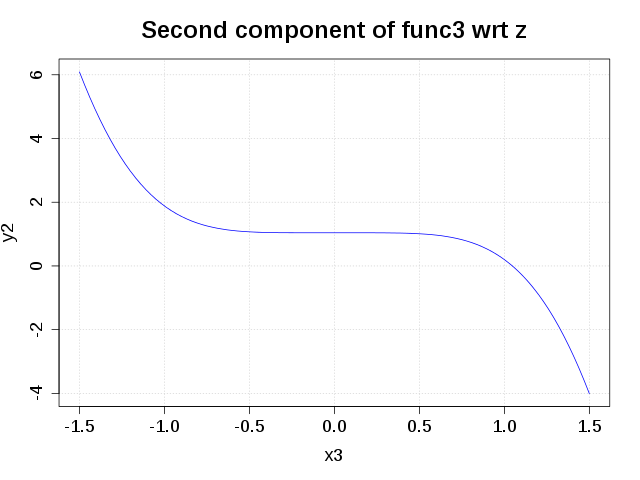
\includegraphics[width=7cm]{Figures/NMFgraph1.png}
                   \caption{Graph of : $ z \mapsto  func3_2(x_0,y_0,z)$, with $(x_0,y_0) = (1.0, 2.0)$ and $z\in [-1.5, 1.5]$.}
                   \label{graph1}
                 \end{center}
               \end{minipage}
               \hfill
               \begin{minipage}{8cm}
                 \begin{center}
                   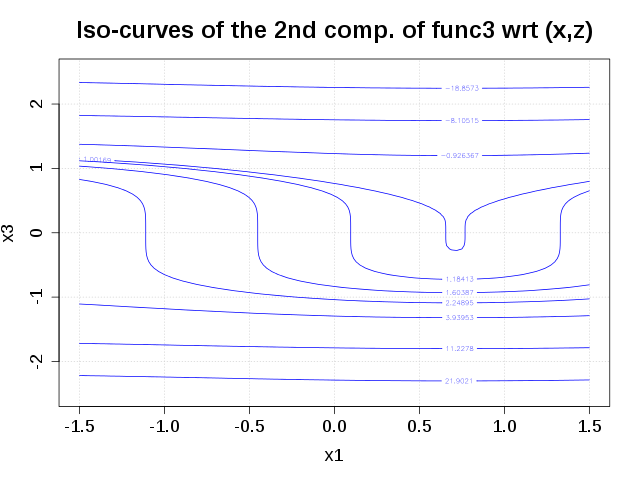
\includegraphics[width=7cm]{Figures/NMFgraph2.png}
                   \caption{Iso-curves of : $ (x,z) \mapsto  func3_2(x_0,y,z)$, with $y_0 = 2.0$ and $x\in [-1.5, 1.5]$ and $z\in [-2.5, 2.5]$.}
                   \label{graph2}
                 \end{center}
               \end{minipage}
             \end{figure}


             \begin{figure}[H]
               \begin{minipage}{8cm}
                 \begin{center}
                   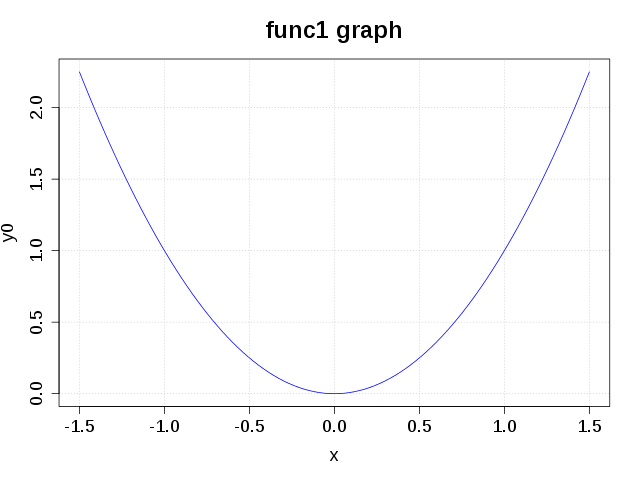
\includegraphics[width=7cm]{Figures/NMFgraph3.png}
                   \caption{Graph of : $ x \mapsto  func1(x)$, with $x\in [-1.5, 1.5]$.}
                   \label{graph1}
                 \end{center}
               \end{minipage}
               \hfill
               \begin{minipage}{8cm}
                 \begin{center}
                   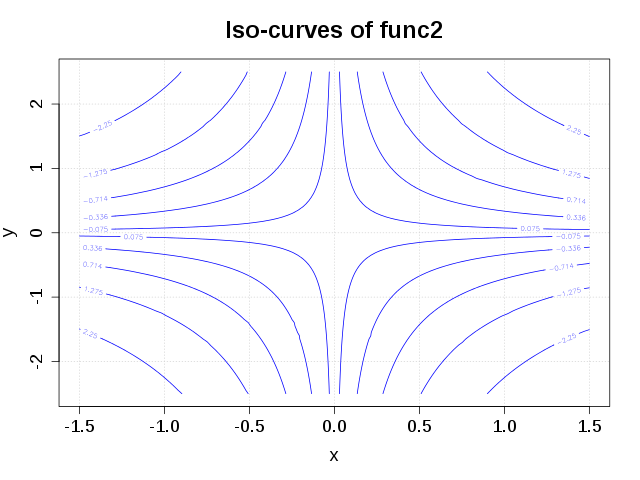
\includegraphics[width=7cm]{Figures/NMFgraph4.png}
                   \caption{Iso-curves of : $ (x,y) \mapsto  func2(x,y)$, with  $x\in [-1.5, 1.5]$ and $y\in [-2.5, 2.5]$.}
                   \label{graph2}
                 \end{center}
               \end{minipage}
             \end{figure}


%%%%%%%%%%%%%%%%%%%%%%%%%%%%%%
\newpage \subsection{Creation of the output variable of interest from the limit state function and the input random  vector}


The objective of the section is to determine the output variable of interest directly from a limit state function and a random input vector declared previously.


% Copyright 2005-2016 Airbus-EDF-IMACS-Phimeca
% Permission is granted to copy, distribute and/or modify this document
% under the terms of the GNU Free Documentation License, Version 1.2
% or any later version published by the Free Software Foundation;
% with no Invariant Sections, no Front-Cover Texts, and no Back-Cover
% Texts.  A copy of the license is included in the section entitled "GNU
% Free Documentation License".
\renewcommand{\filename}{docUC_OVI_FromLSF.tex}
\renewcommand{\filetitle}{UC : Creation of the ouput random vector}

% \HeaderNNIILevel
% \HeaderIILevel
\HeaderIIILevel

\label{CompositeRandomVector}


\index{Random Vector!Output random vector}

The objective of this Use Case is to create the ouput random variable of interest defined as the image through the limit state function of the input random vector.\\

Details on the definition of random mixture variables may be found in the Reference Guide (\extref{ReferenceGuide}{see files Reference Guide - Step B -- Random Mixture : affine combination of independent univariate distributions}{stepB}).\\

\requirements{
  \begin{description}
  \item[$\bullet$] the limit state function : {\itshape myFunction}
  \item[type:]  NumericalMathFunction
  \item[$\bullet$] the random input vector : {\itshape inputRV}
  \item[type:] RandomVector which implementation is a UsualRandomVector
  \end{description}
}
             {
               \begin{description}
               \item[$\bullet$] the output variable of interest {\itshape outputRV = myFunction(inputRV)}
               \item[type:] RandomVector which implementation is a CompositeRandomVector
               \end{description}
             }

             \textspace\\
             Python script for this UseCase :

             \inputscript{script_docUC_OVI_FromLSF}

\newpage % Copyright 2005-2016 Airbus-EDF-IMACS-Phimeca
% Permission is granted to copy, distribute and/or modify this document
% under the terms of the GNU Free Documentation License, Version 1.2
% or any later version published by the Free Software Foundation;
% with no Invariant Sections, no Front-Cover Texts, and no Back-Cover
% Texts.  A copy of the license is included in the section entitled "GNU
% Free Documentation License".
\renewcommand{\filename}{docUC_OVI_RVExtraction.tex}
\renewcommand{\filetitle}{UC : Extraction of a random subvector from a random vector}

% \HeaderNNIILevel
% \HeaderIILevel
\HeaderIIILevel


\index{Random Vector!Extracting a sub vector}

The objective of this Use Case is to extract a subvector from a random vector which has been defined as well  as a UsualRandomvector (it means thanks to a distribution, see UC. \ref{UsualRandomVector}) than  as a CompositeRandomVector (as the image through a limit state function of an input  random vector, see UC. \ref{CompositeRandomVector}).\\

Let's note $\vect{Y} = (Y_1, \cdots, Y_n)$ a random vector and $I \subset [1, n]$ a set of indices :
\begin{itemize}
\item In the first case, the subvector is defined by $\vect{\tilde{Y}} = (Y_i)_{i \in I}$,
\item In the second case, where $\vect{Y} = f(\vect{X})$ with $f = (f_1, \cdots, f_n)$, $f_i$ some scalar functions, the sub vector is $\vect{\tilde{Y}} = (f_i(\vect{X}))_{i \in I}$.
\end{itemize}


\noindent%
\requirements{
  \begin{description}
  \item[$\bullet$] the random vector : {\itshape myRandomVector}
  \item[type:] RandomVector which implementation is a UsualRandomVector or CompositeRandomVector
  \end{description}
}
             {
               \begin{description}
               \item[$\bullet$] the extracted random vector : {\itshape myExtractedRandomVector}
               \item[type:] RandomVector which implementation is a UsualRandomVector or CompositeRandomVector
               \end{description}
             }

             \textspace\\
             Python script for this UseCase :


             \begin{lstlisting}

               # CASE 1 : Get the marginal of the random vector
               # Corresponding to the component i

               # Care : numerotation begins at 0
               myExtractedRandomVector = myRandomVector.getMarginal(i)


               # CASE 2 : Get the marginals of the random vector
               # Corresponding to several components
               # decribed in the myIndice table
               # For example, components 0, 1, and 5

               myExtractedRandomVector = myRandomVector.getMarginal( (0, 1, 5) )
             \end{lstlisting}



%%%%%%%%%%%%%%%%%%%%%%%%%%%%%%
\newpage \subsection{Creation of the output variable of interest defined as an affine combination of input random variables}


% Copyright (C) 2005-2015 Airbus - EDF - IMACS - Phimeca
% Permission is granted to copy, distribute and/or modify this document
% under the terms of the GNU Free Documentation License, Version 1.2
% or any later version published by the Free Software Foundation;
% with no Invariant Sections, no Front-Cover Texts, and no Back-Cover
% Texts.  A copy of the license is included in the section entitled "GNU
% Free Documentation License".
\renewcommand{\filename}{docUC_OVI_RandomMixture.tex}
\renewcommand{\filetitle}{UC : Creation of a Random Mixture}

% \HeaderNNIILevel
% \HeaderIILevel
\HeaderIIILevel


\index{Random Vector!Output random vector}
\index{Distribution!Random Mixture}

The objective of this Use Case is to define a random vector $\vect{Y}$ as a RandomMixture, which means an affine transform of input random variables :
\begin{align*}
  \displaystyle \vect{Y}=\vect{y}_0+\mat{M}\,\vect{X}
\end{align*}
where $\vect{y}_0\in\mathbb{R}^d$ is a deterministic vector with $d\in\{1,2,3\}$, $\mat{M}\in\mathcal{M}_{d,n}(\mathbb{R})$ a deterministic matrix and $(X_k)_{ 1 \leq k \leq n}$ are some \emph{independent univariate} variables.\\

Be careful! This notion is different from the Mixture notion where the combination is made on the probability density functions and not on the univariate random variable :
\begin{itemize}
\item Random Mixture (in dimension 1) : $Y = a_0 + \sum_{i=1}^n a_i X_i$,
\item Mixture : $p_Y = \sum_{i=1}^n a_i p_{X_i}$, where $p_{X_i}$ is the probability density function of $X_i$ and $\sum_{i=1}^n a_i = 1$.
\end{itemize}

When not precised, the coefficient $\vect{y}_0$ is taken equal to $0$.\\



OpenTURNS evaluates the probability density function and cumulative distribution function of the random variable $\vect{Y}$. So, it is possible to ask $\vect{Y}$ any request compatible with a {\itshape Distribution}: moments, quantiles(in dimension 1 only), PDF and CDF evaluations, ...\\

It is important to note that the distribution evaluation of $\vect{Y}$ needs the evaluation of the characteristic functions of the univariate $X_i$. OpenTURNS proposes an implementation of all its univariate distributions, continuous or discrete ones. But only some of the them have the implementation of a specific algorithm that evaluates the characteristic function : it is the case of all the discrete distributions and most of (but not all) the continuous ones. In that case, the evaluation is performant. For the remaining distributions, the generic implementation might be time consuming for high arguments. \\

Furthermore, let's note that as $\vect{Y}$ is \emph{not} a {\itshape CompositeRandomVector}; In dimension 1, it cannot be used by a FORM/SORM algorithm, a QuadraticCumul algorithm or even a Simulation algorithm... In order to use such algorithms, it is necessary to transform the {\itshape RandomMixture} in a {\itshape CompositeRandomVector} by using the identity function $f : \Rset \rightarrow \Rset$ quickly defined (see the following python script).\\

The example here is an output variable of interest defined as the following combination :
\begin{align*}
  Y = 2 + 5X_1 + X_2
\end{align*}
where :
\begin{itemize}
\item  $X_1$ follows a $\cE(\lambda = 1.5)$,
\item  $X_2$ follows a $\cN(\mu = 4,Variance = 1)$.
\end{itemize}

The UC asks $Y$ its mean, variance, probability density graph, quantile of order $90\%$, its probability to exceeds 3.



\noindent%
\requirements{
  \begin{description}
  \item[$\bullet$] none
  \end{description}
}
             {
               \begin{description}
               \item[$\bullet$] the random mixture $Y$ : {\itshape myRandomMixtureY}
               \item[type:] RandomMixture
               \end{description}
             }

             \textspace\\
             Python script for this UseCase :

             \inputscript{script_docUC_OVI_RandomMixture}

             \textspace\\


             \begin{figure}[H]
               \begin{minipage}{8cm}
                 \begin{center}
                   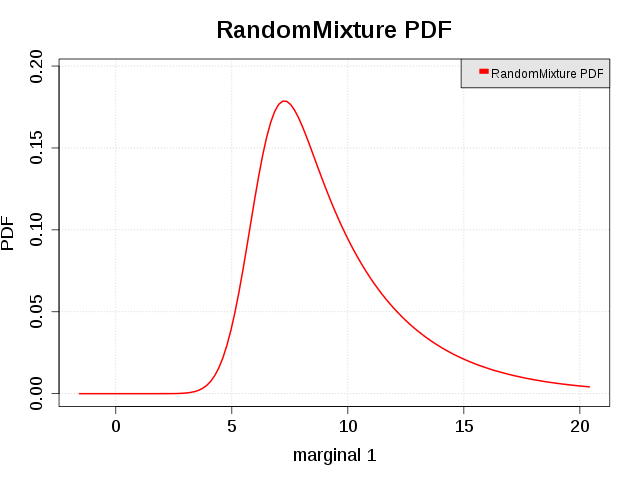
\includegraphics[width=8cm]{Figures/RandomMixture_pdf.png}
                   \caption{Probability density function of a Random Mixture.}
                   \label{PDFRandomMixture}
                 \end{center}
               \end{minipage}
               \hfill
               \begin{minipage}{8cm}
                 \begin{center}
                   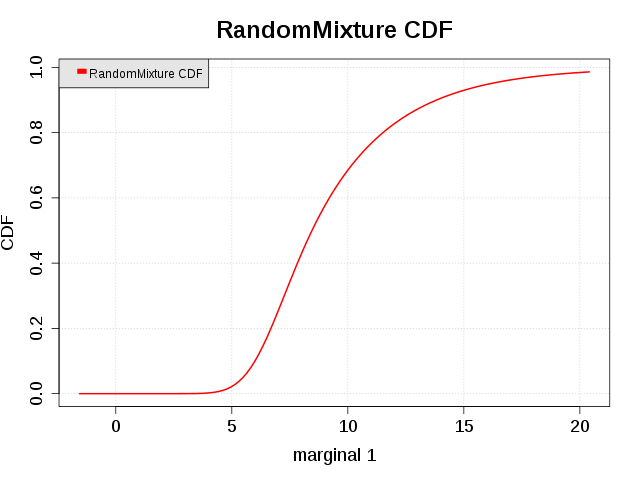
\includegraphics[width=8cm]{Figures/RandomMixture_cdf.png}
                   \caption{Cumulative density function of a Random Mixture.}
                   \label{CDFRandomMixture}
                 \end{center}
               \end{minipage}
             \end{figure}




%%%%%%%%%%%%%%%%%%%%%%%%%%%%%%
\newpage \subsection{Creation of the output variable of interest from the result of a polynomial chaos expansion}

% Copyright 2005-2016 Airbus-EDF-IMACS-Phimeca
% Permission is granted to copy, distribute and/or modify this document
% under the terms of the GNU Free Documentation License, Version 1.2
% or any later version published by the Free Software Foundation;
% with no Invariant Sections, no Front-Cover Texts, and no Back-Cover
% Texts.  A copy of the license is included in the section entitled "GNU
% Free Documentation License".
\renewcommand{\filename}{docUC_OVI_PolyChaosExp.tex}
\renewcommand{\filetitle}{UC : Creation of the output variable of interest from the result of a polynomial chaos expansion}

% \HeaderNNIILevel
% \HeaderIILevel
\HeaderIIILevel


\label{RandomVectorPolynomialChaos}



\index{Random Vector!Output random vector}

The objective of this Use Case is to define the output variable of interest as the result of a polynomial chaos algorithm which defined a particular response surface (refer to \ref{polynomialchaosexpansion}).\\

Details on the polynomial chaos expansion may be found in the Reference Guide (\extref{ReferenceGuide}{see files Reference Guide - Step Resp. Surf. -- Polynomial Chaos Expansion}{responseSurface}).\\


\requirements{
  \begin{description}
  \item[$\bullet$] the result structure of a polynomial chaos algorithm : {\itshape polynomialChaosResult}
  \item[type:] a FunctionalChaosResult
  \end{description}
}
             {
               \begin{description}
               \item[$\bullet$] the new output variable of interest : {\itshape newOuputVariableOfInterest}
               \item[type:] a RandomVector
               \end{description}
             }

             \textspace\\
             Python script for this UseCase :

             \begin{lstlisting}
               # Create the new ouput variable of interest
               # based on the meta model
               # evaluated from the polynomial chaos algorithm
               newOuputVariableOfInterest = RandomVector(polynomialChaosResult)
             \end{lstlisting}

\newpage % Copyright 2005-2016 Airbus-EDF-IMACS-Phimeca
% Permission is granted to copy, distribute and/or modify this document
% under the terms of the GNU Free Documentation License, Version 1.2
% or any later version published by the Free Software Foundation;
% with no Invariant Sections, no Front-Cover Texts, and no Back-Cover
% Texts.  A copy of the license is included in the section entitled "GNU
% Free Documentation License".
\renewcommand{\filename}{docUC_OVI_SpecializedPolyChaosExp.tex}
\renewcommand{\filetitle}{UC : Creation of a specialized random vector for the global sensitivity analysis using a polynomial chaos expansion}

% \HeaderNNIILevel
% \HeaderIILevel
\HeaderIIILevel

\label{FunctionalChaosRandomVector}

\index{Random Vector!Output random vector}

The objective of this Use Case is to define the output variable of interest as a specialized random vector that allows the User to compute the mean and covariance using the coefficients of the  decomposition upon the polynomial hilbertian basis, and also the Sobol indices and total indices.\\


Details on the Sobol indices may be found in the Reference Guide (\extref{ReferenceGuide}{see files Reference Guide - Step C' -- Sensitivity analysis using Sobol indices}{stepCprime}).\\

If $g : \Rset^n \longrightarrow \Rset$ is a model and $Y = g(\vect{X}$ is the random ouput variable with $\vect{X}$ a random vector, we define the Sobol indice associated to $\vect{i} = (i_1, \dots, i_k) )$ as follows where we suppose $g$ and $\vect{X}$ have the good properties :
\begin{align*}
  IS(\vect{i}) = \displaystyle \frac{\Var{\Expect{Y|X_{i_1} \dots X_{i_k}}}}{\Var{Y}}
\end{align*}

The Total Sobol indice associated to $(i_1, \dots, i_k) )$ is defined as :
\begin{align*}
  \displaystyle TIS(\vect{i}) = \sum_{\vect{j} \in I(\vect{i})} IS(\vect{j}
\end{align*}
where $I(\vect{i}) = \left\{ (j_1, \dots, j_p), \, p \in [k,n]/ \{i_1, \dots, i_k\} \subset  \{j_1, \dots, j_p\}  \right\}$.\\



\requirements{
  \begin{description}
  \item[$\bullet$] the result structure of a polynomial chaos algorithm : {\itshape polynomialChaosResult}
  \item[type:] a FunctionalChaosResult
  \end{description}
}
             {
               \begin{description}
               \item[$\bullet$] the new output variable of interest : {\itshape newOuputVariableOfInterest}
               \item[type:] a FunctionalChaosRandomVector
               \end{description}
             }

             \textspace\\
             Python script for this UseCase :

             \begin{lstlisting}
               # Create the new ouput variable of interest
               # based on the meta model
               # evaluated from the polynomial chaos algorithm
               # in a way that allow to compute Sobol indices
               # and total indices
               newOuputVariableOfInterest = FunctionalChaosRandomVector(polynomialChaosResult)
               print "Sobol index 0=", newOuputVariableOfInterest.getSobolIndex(0)
               indices = Indices(2)
               indices[0] = 0
               indices[1] = 1
               print "Sobol index [0, 1]=", newOuputVariableOfInterest.getSobolIndex(indices)
               print "Sobol total index 0=", newOuputVariableOfInterest.getSobolTotalIndex(0)
               indices = Indices(2)
               indices[0] = 0
               indices[1] = 1
               print "Sobol total index [0, 1]=", newOuputVariableOfInterest.getSobolTotalIndex(indices)

             \end{lstlisting}


%%%%%%%%%%%%%%%%%%%%%%%%%%%%%%%%%%%%%%%%%%%%%%%%%%%%%%%%%%%%%%%%%%%%%%%%%%%%%%%%%%%%%%%%%%
\newpage \section{Uncertainty propagation and Uncertainty sources ranking}

The objective of this section is to manipulate all the functionalities to propagate uncertainties from the random input vector through the limit state function until the output variable of interest
(\extref{ReferenceGuide}{see Reference Guide - Global Methodology for an uncertainty stdy - Part C : propagating uncertainty sources}{stepC}).

Some techniques require the generation of random distributed sequences and others some low discrepancy sequences.

% Copyright 2005-2016 Airbus-EDF-IMACS-Phimeca
% Permission is granted to copy, distribute and/or modify this document
% under the terms of the GNU Free Documentation License, Version 1.2
% or any later version published by the Free Software Foundation;
% with no Invariant Sections, no Front-Cover Texts, and no Back-Cover
% Texts.  A copy of the license is included in the section entitled "GNU
% Free Documentation License".
\renewcommand{\filename}{docUC_RandomGenerator.tex}
\renewcommand{\filetitle}{UC : Parametrisation of the Random Generator}

% \HeaderNNIILevel
\HeaderIILevel
% \HeaderIIILevel

\label{randomGenerator}


\index{Random Generator}

The seed of the random generator is automatically initialized to 0. It means that as soon as a the openturns session is launched, the sequence of random values generated within $[0,1]$ is the same one : if a script is launched several times, within different openturns sessions, the same results will be obtained. \\


Details on the random generator may be found in the Reference Guide (\extref{ReferenceGuide}{see files Reference Guide - Step B -- Uniform Random Generator}{stepB}).\\


Before any simulation, it is possible to initialise differently than the value by default or get the state of the random generator. \\
To initialize the random generator state, it is possible :
\begin{itemize}
\item to use an easy procedure thanks to the method {\itshape SetSeed()}  parameterized with an integer in $[0, 2^{32}-1]$ :
  \begin{itemize}
  \item to obtain a reproductible sequence of generated random values, we need to explicitely give a deterministic integer,
  \item to obtain a non reproductible sequence of generated random values (it means a new one each time the openturns session is launched), we can give a random integer, determined thanks to the time of the day or the number of the current python session.
  \end{itemize}
\item to specify a complete state of the random generator, usually previously obtained thanks to the {\itshape GetState()} method.
\end{itemize}


\begin{lstlisting}
  # INITIALIZE THE RANDOM GENERATOR STATE

  # Case 1 : reproductible sequence of generated random vector
  # the seed is reproductible

  # Initialise the state of the random generator
  # thanks to the fonctionality SetSeed(n) where n is an UnsignedLong in [0, 2^(32)-1]
  # which enables an easy initialisation for the user
  RandomGenerator.SetSeed(77)

  # or by specifying a complete state of the random generator : particularState
  # coming from a previous particularState = RandomGenerator.GetState() :
  RandomGenerator.SetState(particularState)

  # Case 2 : non reproductible sequence of generated random vector
  # the seed is not reproductible

  # Example 1 : the number of the openturns python session
  from os import getpid
  RandomGenerator.SetSeed(getpid())

  # Example 2 : times of the moment
  from os import times
  RandomGenerator.SetSeed(int(100*times()[4]))


  # GET THE RANDOM GENERATOR STATE

  # Get the complete state of the random generator before simulation
  randomGeneratorStateBeforeRandomExperiment = RandomGenerator.GetState()
\end{lstlisting}

\newpage % Copyright (C) 2005-2015 Airbus - EDF - IMACS - Phimeca
% Permission is granted to copy, distribute and/or modify this document
% under the terms of the GNU Free Documentation License, Version 1.2
% or any later version published by the Free Software Foundation;
% with no Invariant Sections, no Front-Cover Texts, and no Back-Cover
% Texts.  A copy of the license is included in the section entitled "GNU
% Free Documentation License".
\renewcommand{\filename}{docUC_LowDiscrepancySequences.tex}
\renewcommand{\filetitle}{UC : Generation of low discrepancy sequences}

% \HeaderNNIILevel
\HeaderIILevel
% \HeaderIIILevel

\label{lowDiscrepancySequence}


\index{Low Discrepancy Sequences}

It is possible to generate some low discrepancy sequences in order to approximate some integrals.\\

Details on low discrepancy sequences  may be found in the Reference Guide (\extref{ReferenceGuide}{Reference Guide - Low Discrepancy Sequence}{discrepancysequence}).



OpenTURNS proposes the following sequences : Sobol, Faure, Halton, Reverse Halton and Haselgrove, in dimension $n \geq 1$.


\requirements{
  \begin{description}
  \item[$\bullet$] -
  \end{description}
}
             {
               \begin{description}
               \item[$\bullet$] a Faure sequence : {\itshape myFaureSeq}
               \item[type:] FaureSequence
               \item[$\bullet$] a Sobol sequence : {\itshape mySobolSeq}
               \item[type:] SobolSequence
               \item[$\bullet$] an Halton sequence: {\itshape myHaltonSeq}
               \item[type:] HaltonSequence
               \item[$\bullet$] an Haselgrove sequence: {\itshape myHaselgroveSeq}
               \item[type:] HaselgroveSequence
               \item[$\bullet$] a Reverse Halton sequence : {\itshape myReverseHaltonSeq}
               \item[type:] ReverseHaltonSequence
               \item[$\bullet$] the points of the sequence : {\itshape myFirstSequencePoints}
               \item[type:] NumericalSample
               \end{description}
             }

             \textspace\\
             Python  script for this UseCase :

             \begin{lstlisting}
               # Create the Faure sequence of dimension 2
               myFaureSeq = FaureSequence(2)

               # Create the Sobol sequence of dimension 2
               mySobolSeq = SobolSequence(2)

               # Create the Halton sequence of dimension 2
               myHaltonSeq = HaltonSequence(2)

               # Create the Haselgrove sequence of dimension 2
               myHaselgroveSeq = HaselgroveSequence(2)

               # Create the Inverse Halton sequence of dimension 2
               myReverseHaltonSeq = ReverseHaltonSequence(2)

               # Generate the first points of the sequence
               myFirstSequencePoints = myFaureSeq.generate(10)
             \end{lstlisting}


             To illustrate these sequences, we generate the first points (1024) from the Sobol, Halton and Reverse Halton schemes. In order to ease the comparaison with the uniformly ditributed sequence, we draw the first points obtained from the Mersenne Twister algorithm : this last sequence has a greater discrepancy than the other ones.



             \begin{figure}[H]
               \begin{minipage}{10cm}
                 \begin{center}
                   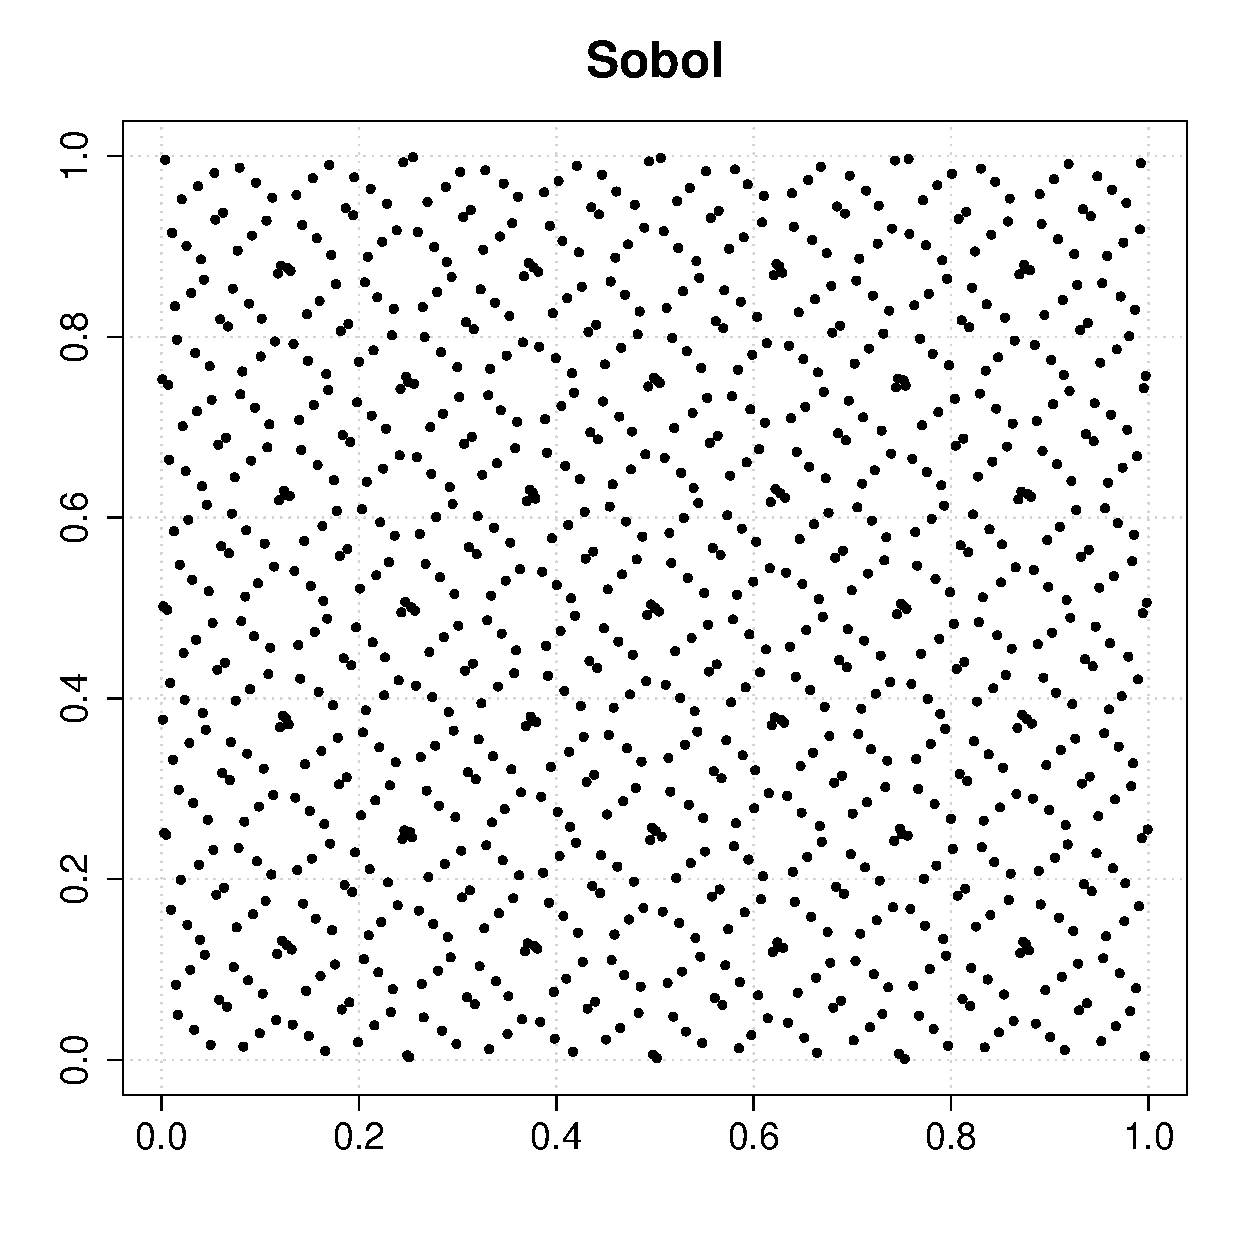
\includegraphics[width=7cm]{Figures/sobol_cloud.pdf}
                   \caption{Sobol sequence.}
                   \label{Sobol}
                 \end{center}
               \end{minipage}
               \hfill
               \begin{minipage}{10cm}
                 \begin{center}
                   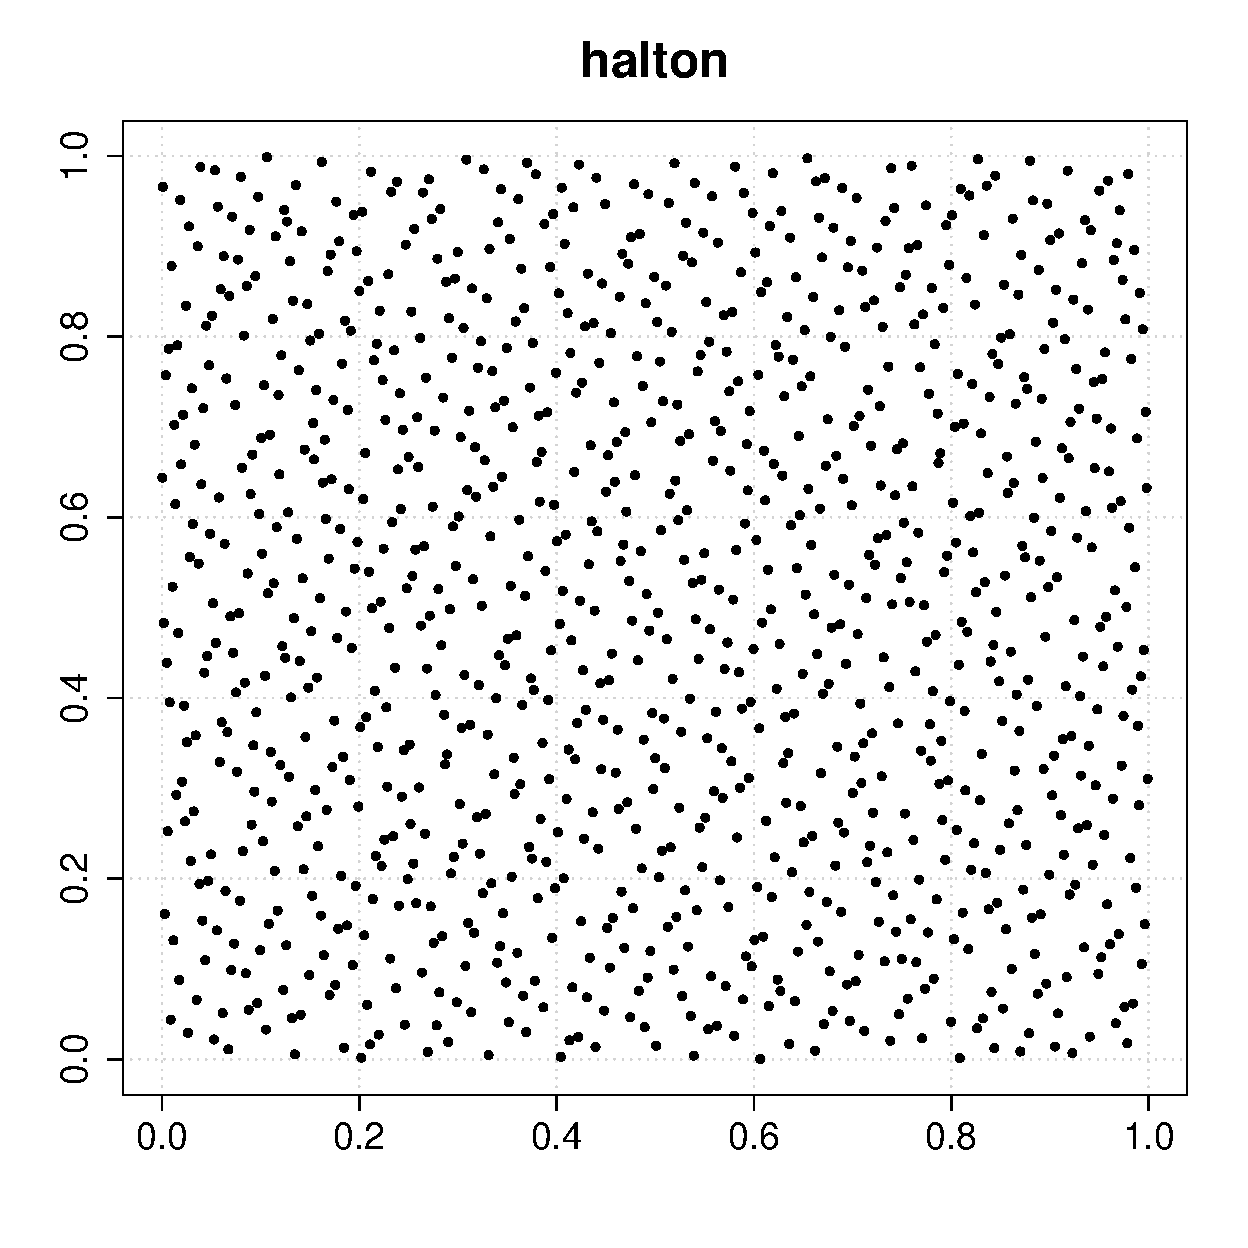
\includegraphics[width=7cm]{Figures/halton_cloud.pdf}
                   \caption{Halton sequence.}
                   \label{Halton}
                 \end{center}
               \end{minipage}
             \end{figure}


             \begin{figure}[H]
               \begin{minipage}{10cm}
                 \begin{center}
                   \includegraphics[width=7cm]{Figures/reverseHalton_cloud.pdf}
                   \caption{Reverse Halton sequence.}
                   \label{ReverseHalton}
                 \end{center}
               \end{minipage}
               \hfill
               \begin{minipage}{10cm}
                 \begin{center}
                   \includegraphics[width=7cm]{Figures/mersenne_twister_cloud.pdf}
                   \caption{Uniform random sequence.}
                   \label{Uniform}
                 \end{center}
               \end{minipage}
             \end{figure}




%%%%%%%%%%%%%%%%%%%%%%%%%%%%%%
\newpage \subsection{Min/Max approach}


In this section, we focus on the deterministic approach which consists of researching the variation range of the output variable of interest.

% Copyright (C) 2005-2015 Airbus - EDF - IMACS - Phimeca
% Permission is granted to copy, distribute and/or modify this document
% under the terms of the GNU Free Documentation License, Version 1.2
% or any later version published by the Free Software Foundation;
% with no Invariant Sections, no Front-Cover Texts, and no Back-Cover
% Texts.  A copy of the license is included in the section entitled "GNU
% Free Documentation License".
\renewcommand{\filename}{docUC_MinMax_DetExperimentPlane.tex}
\renewcommand{\filetitle}{UC : Creation of a deterministic design of experiments  : Axial, Box, Composite, Factorial patterns}

% \HeaderNNIILevel
% \HeaderIILevel
\HeaderIIILevel

\label{determExpPlane}



\index{Design of Experiments !Factorial scheme}
\index{Design of Experiments !Composite scheme}
\index{Design of Experiments !Axial scheme}
\index{Design of Experiments !Box scheme}
\index{Design of Experiments !Scaling}
\index{Design of Experiments !Translation}

The objective of this Use Case is to create an design of experiments  which scheme is specified and then denoted {\itshape deterministic} design of experiments .\\


Details on design of experiments  may be found in the Reference Guide (\extref{ReferenceGuide}{see files Reference Guide - Step C -- Min-Max approach using Designs Of Experiment}{stepC}).\\

OpenTURNS enables to define four types of deterministic design of experiments : axial, composite, factorial and box.\\

In order to define an design of experiments , follow the 3  steps, whatever the type of the design of experiments , where $n$ is the dimension of the space and $n_{level}$ the number of levels (the same for each direction except for the Box grid) :
\begin{itemize}
\item Step 1 : Define a reduced and centered grid structure, centered on $\vect{0} \in \Rset^n$, by specifying the levels which will be consider on each direction,
\item Step 2 : Scale each direction with a specific scale factor for each direction, in order to give a unit effect on each direction,
\item Step 3 : Translate the scaled grid structure onto a specified center point.
\end{itemize}

Each design of experiments  has a specific method to define its reduced and centered grid structure :
\begin{itemize}
\item {\bf Axial}: the  points grid is obtained by discretizing each direction according to the specified levels, symmetrically with respect to 0. The number of points generated is $1 + 2n* n_{level}$.
\item {\bf Factorial}: the  points grid is obtained by discretizing each principal diagonal according to the specified levels, symmetrically with respect to 0. The number of points generated is $1 +  2^n*n_{level}$.
\item {\bf Composite}: the  points grid is obtained as the union between an axial and a factorial design of experiments . The number of points generated is $1 + 2n*n_{level} +  2^n*n_{level}$.
\item {\bf Box}: the  points grid is obtained by regularly discretizing the unit pavement $[0, 1]^n$, with the number of intermediate points specified for each direction.  The number of points generated is $\displaystyle \prod_{i=1}^{n} (2+n_{level}(direction \, \, i))$.
\end{itemize}

In order to scale each direction according to a specified factor or/and to translate the points grid until a specified center, the methods {\itshape scale} and {\itshape translate} must be used.\\

The following example works in $\Rset^2$.\\

\requirements{
  \begin{description}
  \item[$\bullet$] none
  \end{description}
}
             {
               \begin{description}
               \item[$\bullet$] a centered and reducted grid structure : {\itshape myCenteredReductedPlane}
               \item[type:] ExperimentPlane, which type is Axial, Composite, Factorial or Box
               \item[$\bullet$] the numerical sample associated to the centered and reducted grid structure then scaled then translated grid structure : {\itshape mySample}
               \item[type:] NumericalSample
               \end{description}
             }

             \textspace\\
             Python script for this UseCase :


             \begin{lstlisting}

               # Define a scale factor for each direction
               scaledVector = NumericalPoint( (1.5, 2.5) )

               # Define the translation until the final center of the design of experiments
               translationVector = NumericalPoint( (2., 3.) )

               # Define the different levels of the grid structure
               # CARE : for the axial, composite and factorial design of experiments,
               # these levels are all applied along each direction
               # Here : 3 levels on each direction
               levels = NumericalPoint( (1., 1.5, 3.) )

               # For the box design of experiments , levels specifies the number of
               # intermediate points on each direction (one per direction)
               # Here : direction 1 will be discretized with 2 intermediate points
               # and direction 2 with 4 intermediate points
               levelsBox = NumericalPoint( (2., 4.) )


               # STEP 1 : Define a reduced and centered grid structure

               # AXIAL structure
               myCenteredReductedGrid = Axial(2,levels)

               # COMPOSITE structure
               myCenteredReductedGrid = Composite(2,levels)

               # FACTORIAL structure
               myCenteredReductedGrid = Factorial(2,levels)

               # BOX structure
               myCenteredReductedGrid = Box(levelsBox)

               # Generate the numerical sample (centered and reducted grid structure)
               # a NumericalSample is created
               mySample = myCenteredReductedGrid.generate()

               # Get the number of points of the centered and reducted grid structure
               pointsNumber = mySample.getSize()


               # STEP 2 : Scale each direction with a specific scale factor

               # The NumericalSample is transformed
               mySample.scale(scaledVector)


               # STEP 3 : Translate the scaled grid structure onto a specified center point

               # The NumericalSample is transformed
               mySample.translate(translationVector)

               # Print the numerical sample
               print mySample
             \end{lstlisting}
             \textspace\\


             Figures \ref{AxialGrid} to \ref{TranslatedScaledBoxGrid} draw the different grid structures obtained after the {\itshape scale} or {\itshape translate} methods.

             \begin{figure}[H]
               \begin{minipage}{10cm}
                 \begin{center}
                   \includegraphics[width=8cm]{Figures/AxialGrid.png}
                   \caption{Axial Design of Experiments  : initial grid.}
                   \label{AxialGrid}
                 \end{center}
               \end{minipage}
               \hfill
               \begin{minipage}{10cm}
                 \begin{center}
                   \includegraphics[width=8cm]{Figures/ScaledAxialGrid.png}
                   \caption{Axial Design of Experiments  : after scaling.}
                   \label{ScaledAxialGrid}
                 \end{center}
               \end{minipage}
             \end{figure}

             \begin{figure}[H]
               \begin{center}
                 \includegraphics[width=8cm]{Figures/TranslatedScaledAxialGrid.png}
               \end{center}
               \caption{Axial Design of Experiments  : after scaling and translation.}
               \label{TranslatedScaledAxialGrid}
             \end{figure}



             \begin{figure}[H]
               \begin{minipage}{10cm}
                 \begin{center}
                   \includegraphics[width=8cm]{Figures/FactorialGrid.pdf}
                   \caption{Factorial Design of Experiments  : initial grid.}
                   \label{FactorialGrid}
                 \end{center}
               \end{minipage}
               \hfill
               \begin{minipage}{10cm}
                 \begin{center}
                   \includegraphics[width=8cm]{Figures/ScaledFactorialGrid.png}
                   \caption{Factorial Design of Experiments  : after scaling.}
                   \label{ScaledFactorialGrid}
                 \end{center}
               \end{minipage}
             \end{figure}




             \begin{figure}[H]
               \begin{center}
                 \includegraphics[width=8cm]{Figures/TranslatedScaledFactorialGrid.png}
               \end{center}
               \caption{Factorial Design of Experiments  : after scaling and translation.}
               \label{TranslatedScaledFactorialGrid}
             \end{figure}





             \begin{figure}[H]
               \begin{minipage}{10cm}
                 \begin{center}
                   \includegraphics[width=8cm]{Figures/CompositeGrid.png}
                   \caption{Composite Design of Experiments  : initial grid.}
                   \label{CompositeGrid}
                 \end{center}
               \end{minipage}
               \hfill
               \begin{minipage}{10cm}
                 \begin{center}
                   \includegraphics[width=8cm]{Figures/ScaledCompositeGrid.png}
                   \caption{Composite Design of Experiments  : after scaling.}
                   \label{ScaledCompositeGrid}
                 \end{center}
               \end{minipage}
             \end{figure}

             \begin{figure}[H]
               \begin{center}
                 \includegraphics[width=8cm]{Figures/TranslatedScaledCompositeGrid.png}
               \end{center}
               \caption{Composite Design of Experiments  : after scaling and translation.}
               \label{TranslatedScaledCompositeGrid}
             \end{figure}


             \begin{figure}[H]
               \begin{minipage}{10cm}
                 \begin{center}
                   \includegraphics[width=8cm]{Figures/BoxGrid.png}
                   \caption{Box Design of Experiments  : initial grid.}
                   \label{BoxGrid}
                 \end{center}
               \end{minipage}
               \hfill
               \begin{minipage}{10cm}
                 \begin{center}
                   \includegraphics[width=8cm]{Figures/ScaledBoxGrid.png}
                   \caption{Box Design of Experiments  : after scaling.}
                   \label{ScaledBoxGrid}
                 \end{center}
               \end{minipage}
             \end{figure}

             \begin{figure}[H]
               \begin{center}
                 \includegraphics[width=8cm]{Figures/TranslatedScaledBoxGrid.png}
               \end{center}
               \caption{Box Design of Experiments  : after scaling and translation.}
               \label{TranslatedScaledBoxGrid}
             \end{figure}

\newpage % Copyright (C) 2005-2015 Airbus - EDF - IMACS - Phimeca
% Permission is granted to copy, distribute and/or modify this document
% under the terms of the GNU Free Documentation License, Version 1.2
% or any later version published by the Free Software Foundation;
% with no Invariant Sections, no Front-Cover Texts, and no Back-Cover
% Texts.  A copy of the license is included in the section entitled "GNU
% Free Documentation License".
\renewcommand{\filename}{docUC_MinMax_CombinatorialGenerators.tex}
\renewcommand{\filetitle}{UC: Creation of a combinatorial generator: subsets, injections, Cartesian products}

% \HeaderNNIILevel
% \HeaderIILevel
\HeaderIIILevel

\label{randomExpPlane}


\index{Design of Experiments !Combinations generator }
\index{Design of Experiments !K-permutations generator }
\index{Design of Experiments !Tuples generator }
\index{Combinatorial generators}

The objective of this Use Case is to define a combinatorial generator, it means a design of experiment able to generate all the integer collections satisfying a given combinatorial constraint.\\


Details on combinatorial generators may be found in the Reference Guide (\extref{ReferenceGuide}{see files Reference Guide - Step C -- Min-Max approach using Designs Of Experiment}{stepC}).\\

OpenTURNS proposes the following combinatorial generators:
\begin{itemize}
\item the Tuples generator, which allows to generate all the elements of a Cartesian product $E=\{0,\hdots,n_0-1\}\times\hdots\times\{0,\hdots,n_{d-1}-1\}$, it means all the points $\vect{x}$ of dimension $d$ with integral components such that $0\leq x_0\leq n_0-1,\hdots,0\leq x_{d-1} \leq n_{d-1}-1$. The integers $n_0,\hdots,n_{d-1}$ are supposed to be positive, if one of them is zero then $E$ is the empty set. The total number of generated points is $N=\prod_{k=0}^{d-1}n_k$.
\item the K-permutations generator, which allows to generate all the injective functions from $\{0,\hdots,k-1\}$ into $\{0,\hdots,n-1\}$, described by a point $\vect{x}$ of dimension $k$ with integral components, such that the associated injective function $\phi$ maps $\ell\in\{0,\hdots,k-1\}$ into $\phi(\ell)=x_{\ell}$. $k$ and $n$ are positive integers such that $k\leq n$, else there is no such injective function. The total number of generated points is $N=\dfrac{n!}{(n-k)!}$.
\item the combinations generator, which allows to generate all the subsets of size $k$ of $\{0,\hdots,n-1\}$. The subsets are described using points $\vect{x}$ with integral components such that $0\leq x_0<\hdots<x_{k-1}\leq n$. If $k>n$, there is no such subset. The total number of generated points is $N=\dfrac{n!}{k!(n-k)!}$.
\end{itemize}

Be aware of the fact that the number of generated points grows very rapidly with the magnitude of the parameters.\\

\requirements{
  \begin{description}
  \item[$\bullet$] the parameters of the combinatorial generator: {\itshape $(n, k)$ or $(n_0,\hdots,n_{d-1})$}
  \item[type:] UnsignedLong
  \end{description}
}
             {
               \begin{description}
               \item[$\bullet$] the sample generated: {\itshape experimentSample}
               \item[type:] IndicesCollection
               \end{description}
             }

             \textspace\\

             Python script for this UseCase :

             \inputscript{script_docUC_MinMax_CombinatorialGenerators}

\newpage % Copyright (C) 2005-2015 Airbus - EDF - IMACS - Phimeca
% Permission is granted to copy, distribute and/or modify this document
% under the terms of the GNU Free Documentation License, Version 1.2
% or any later version published by the Free Software Foundation;
% with no Invariant Sections, no Front-Cover Texts, and no Back-Cover
% Texts.  A copy of the license is included in the section entitled "GNU
% Free Documentation License".
\renewcommand{\filename}{docUC_MinMax_RandomExperimentPlane.tex}
\renewcommand{\filetitle}{UC: Creation of a random design of experiments : Monte Carlo, LHS patterns}

% \HeaderNNIILevel
% \HeaderIILevel
\HeaderIIILevel

\label{randomExpPlane}


\index{Design of Experiments !Monte Carlo design of experiments }
\index{Design of Experiments !LHS design of experiments }
\index{Random Generator}

The objective of this Use Case is to define a random design of experiments  : the design of experiments  does not follow a specified scheme any more. The experiment grid is generated according to a specified distribution and a specified number of points.\\


Details on design of experiments  may be found in the Reference Guide (\extref{ReferenceGuide}{see files Reference Guide - Step C -- Min-Max approach using Designs Of Experiment}{stepC}).\\


OpenTURNS proposes many sampling methods to generate the experiment grid, two of them will be detailed here:
\begin{itemize}
\item the Monte Carlo method: the numerical sample is generated by sampling the specified distribution. When recalled, the {\itshape generate} method regenerates a new numerical sample.
\item the LHS method: the numerical sample is generated by sampling the specified distribution with the LHS technique:  some cells are determined, with the same probabilistic content according to the specified distribution, each line and each column contains exactly one cell, then points are selected among these selected cells. When recalled, the {\itshape generate} method regenerates a new numerical sample: the point selection within the cells changes but not the cells selection. To change the cell selection, it is necessary to create a new LHS Experiment.
\end{itemize}

Before any simulation, it is usefull to initialize the state of the random generator, as defined in the Use Case \ref{randomGenerator}.\\

\requirements{
  \begin{description}
  \item[$\bullet$] the specified distribution: {\itshape distribution}
  \item[type:] Distribution
  \item[$\bullet$] the number of points of the design of experiments : {\itshape number}
  \item[type:] UnsignedLong
  \end{description}
}
             {
               \begin{description}
               \item[$\bullet$] the sample generated: {\itshape experimentSample}
               \item[type:] NumericalSample
               \end{description}
             }

             \textspace\\
             Python script for this UseCase:

             \begin{lstlisting}
               # Create a Monte Carlo design of experiments
               myRandomExp = MonteCarloExperiment(distribution, number)

               # Create a LHS design of experiments
               myRandomExp = LHSExperiment(distribution, number)

               # Generate the design of experiments  numerical sample
               experimentSample = myRandomExp.generate()
             \end{lstlisting}

\newpage % Copyright (C) 2005-2015 Airbus - EDF - IMACS - Phimeca
% Permission is granted to copy, distribute and/or modify this document
% under the terms of the GNU Free Documentation License, Version 1.2
% or any later version published by the Free Software Foundation;
% with no Invariant Sections, no Front-Cover Texts, and no Back-Cover
% Texts.  A copy of the license is included in the section entitled "GNU
% Free Documentation License".
\renewcommand{\filename}{docUC_MinMax_SpecifiedExperimentPlane.tex}
\renewcommand{\filetitle}{UC : Re-use of a specified numerical sample as design of experiments }

% \HeaderNNIILevel
% \HeaderIILevel
\HeaderIIILevel

\label{fixedExpPlane}


\index{Design of Experiments !Fixed design of experiments }

The objective of this Use Case is to enable to re-use a design of experiments , previously elaborated.\\

Details on design of experiments   may be found in the Reference Guide (\extref{ReferenceGuide}{see files Reference Guide - Step C -- Min-Max approach using Design of Experimentss }{stepC}).\\


This functionality is particularly interesting in the polynomial chaos technique, where the evaluation of the coefficients by regression requires the discretisation of a particular integral : to do that, the User may want to re-use a pre-existing numerical sample (for example, the sparse Smolyak grid) to parameterize algorithms which work with design of experiments  structure (and not numerical sample one).\\

When recalled, the {\itshape generate} method regives the specified numerical sample.\\


\requirements{
  \begin{description}
  \item[$\bullet$] the previously elaborated  numerical sample : {\itshape mySample}
  \item[type:] NumericalSample
  \end{description}
}
             {
               \begin{description}
               \item[$\bullet$] the experiment based on the numerical sample : {\itshape myFixedExperiment}
               \item[type:] FixedExperiment
               \end{description}
             }

             \textspace\\
             Python script for this UseCase :

             \begin{lstlisting}
               # Create a fixed design of experiments
               myFixedExperiment = FixedExperiment(mySample)
             \end{lstlisting}

\newpage % Copyright (C) 2005-2015 Airbus - EDF - IMACS - Phimeca
% Permission is granted to copy, distribute and/or modify this document
% under the terms of the GNU Free Documentation License, Version 1.2
% or any later version published by the Free Software Foundation;
% with no Invariant Sections, no Front-Cover Texts, and no Back-Cover
% Texts.  A copy of the license is included in the section entitled "GNU
% Free Documentation License".
\renewcommand{\filename}{docUC_MinMax_MixedDetRandExperimentPlane.tex}
\renewcommand{\filetitle}{UC : Creation of a mixed deterministic / random design of experiments }

% \HeaderNNIILevel
% \HeaderIILevel
\HeaderIIILevel

\label{determRandomExpPlane}

\index{Design of Experiments !Axial scheme}
\index{Design of Experiments !Mixed deterministic / random design of experiments }
\index{Design of Experiments !Scaling scheme}
\index{Design of Experiments !Translation scheme}

The objective of this Use Case is to  create a deterministic design of experiments  which levels are defined from the probabilistic distribution of the input random vector.\\


Details on design of experiments   may be found in the Reference Guide (\extref{ReferenceGuide}{see files Reference Guide - Step C -- Min-Max approach using Design of Experimentss }{stepC}).\\

The example here is an axial design of experiments  where levels are proportionnal to the standard deviation of each component of the random input vector, and centered on the mean vector of the random input vector. Be carefull to remain within the range of the distribution if the latter is bounded!\\
There are three levels  : +/-1, +/-2, +/-3 around a center fixed equal to the center point ($\vect{0}$).\\
The dilatation vector is composed of the standard deviation of each component of the random input vector.\\

\requirements{
  \begin{description}
  \item[$\bullet$] the input vector : {\itshape input}
  \item[type:] RandomVector
  \end{description}
}
             {
               \begin{description}
               \item[$\bullet$] an design of experiments  : {\itshape myPlane}
               \item[type:] Axial
               \item[$\bullet$] a sample of {\itshape input} according to {\itshape myPlane}: {\itshape inputSample}
               \item[type:] NumericalSample
               \end{description}
             }

             \textspace\\
             Python script for this UseCase :

             \begin{lstlisting}
               # In order to use the 'sqrt' function
               from math import *

               # Dimension of the use case : 4
               dim = 4

               # Give the levels of the design of experiments
               # here,  3 levels : +/-1, +/-2, +/-3
               levelsNumber = 3
               levels = NumericalPoint( (1., 2. 3.) )
               levels.setName( "Levels" )

               # Create the axial plane centered on the vector (0)
               # and with the levels 'levels'
               myPlane = Axial(dim, levels)

               # Generate the points according to the structure
               # of the design of experiments  (in a reduced centered space)
               inputSample = myPlane.generate()

               # Scale the structure of the design of experiments
               # proportionnally to the standard deviation of each component
               # of 'input' in case of a RandomVector
               # Scaling vector for each dimension of the levels of the structure
               # to take into account the dimension of each component
               scaling = NumericalPoint(dim, 0)
               scaling[0] = sqrt(input.getCovariance()[0,0])
               scaling[1] = sqrt(input.getCovariance()[1,1])
               scaling[2] = sqrt(input.getCovariance()[2,2])
               scaling[3] = sqrt(input.getCovariance()[3,3])
               inputSample.scale(scaling)

               # Translate the nonReducedSample onto the center of the design of experiments
               # Translation vector for each dimension
               center = input.getMean()
               inputSample.translate(center)
             \end{lstlisting}

\newpage % Copyright (C) 2005-2015 Airbus - EDF - IMACS - Phimeca
% Permission is granted to copy, distribute and/or modify this document
% under the terms of the GNU Free Documentation License, Version 1.2
% or any later version published by the Free Software Foundation;
% with no Invariant Sections, no Front-Cover Texts, and no Back-Cover
% Texts.  A copy of the license is included in the section entitled "GNU
% Free Documentation License".
\renewcommand{\filename}{docUC_MinMax_ExpPlaneDrawing.tex}
\renewcommand{\filetitle}{UC : Drawing an design of experiments  in dimension 2 }

% \HeaderNNIILevel
% \HeaderIILevel
\HeaderIIILevel

\index{Design of Experiments !Drawing}
\index{Graph Manipulation!View}




The objective of this Use Case is to draw an design of experiments  in dimension 2.\\


\requirements{
  \begin{description}
  \item[$\bullet$] the points of an design of experiments  : {\itshape mySample}
  \item[type:] a NumericalSample
  \end{description}
}
             {
               \begin{description}
               \item[$\bullet$] the files containing the graph, in format .EPS, .FIG, .PNG : {\itshape DoE}
               \item[type:] -
               \end{description}
             }

             \textspace\\
             Python script for this UseCase :


             \begin{lstlisting}
               # Draw it
               from openturns.viewer import View
               mySampleDrawable = Cloud(mySample, "blue", "square", "My design of experiments")
               graph = Graph("My design of experiments", "x", "y", True)
               graph.add(mySampleDrawable)
               view = View(graph)
               view.save('DoE.png')
               view.show()

               # In order to see the drawable without creating the associated files
               # CARE : it requires to have created the graph structure before
               View(mySampleDrawable).show()
               # or to see the graph without creating the associated files
               View(graph).show()
             \end{lstlisting}

\newpage % Copyright 2005-2016 Airbus-EDF-IMACS-Phimeca
% Permission is granted to copy, distribute and/or modify this document
% under the terms of the GNU Free Documentation License, Version 1.2
% or any later version published by the Free Software Foundation;
% with no Invariant Sections, no Front-Cover Texts, and no Back-Cover
% Texts.  A copy of the license is included in the section entitled "GNU
% Free Documentation License".
\renewcommand{\filename}{docUC_MinMax_Evaluation.tex}
\renewcommand{\filetitle}{UC : Min/Max research  from an design of experiments  and sensitivity analysis}

% \HeaderNNIILevel
% \HeaderIILevel
\HeaderIIILevel

\index{Min-Max!}
\index{Sensitivity Analysis!Min-Max}


The objective of this Use Case is to evaluate the min and max values of the output variable of interest from a numerical sample and to evaluate the gradient of the limit state function defining the output variable of interest at a particular point. \\

Details on design of experiments   may be found in the Reference Guide (\extref{ReferenceGuide}{see files Reference Guide - Step C -- Min-Max approach using Design of Experimentss }{stepC}).\\

The numerical sample of the output variable of interest may be obtained as follows :
\begin{itemize}
\item create an design of experiments  of the input random vector : deterministic scheme (see Use Case \ref{determExpPlane}) or random scheme (see Use Case \ref{randomExpPlane}), mixed deterministic/random scheme (see Use Case \ref{determRandomExpPlane}), or by re-using a previously elaborated design of experiments  (see Use Case \ref{fixedExpPlane}),
\item evaluate the output variable of interest on each point of the design of experiments .
\end{itemize}

The example here is the limit state function {\itshape poutre} defined in Eq.(\ref{equatPoutre}) with the random input vector $(E,F,L,I)$.\\

\requirements{
  \begin{description}
  \item[$\bullet$] the numerical sample of the input random vector : {\itshape inputSample}
  \item[type:] NumericalSample
  \item[$\bullet$] the limit state function : {\itshape poutre}
  \item[type:] NumericalMathFunction
  \item[$\bullet$] the input vector where gradient is evaluated : {\itshape input0}
  \item[type:] NumericalPoint
  \end{description}
}
             {
               \begin{description}
               \item[$\bullet$] the min and max of the output variable of interest
               \item[type:] NumericalPoint
               \item[$\bullet$] the deterministic gradient of the output variable of interest at $input_0$
               \item[type:] Matrix
               \end{description}
             }

             \textspace\\
             Python script for this UseCase :

             \begin{lstlisting}
               # Generate the  values of the output variable of interest
               # 'output = poutre(input)' corresponding to 'inputSample'
               outputSample = poutre(inputSample)
               print "outputSample = ", outputSample

               # Get the min and the max of the output variable, component by component
               min = outputSample.getMin()
               max = outputSample.getMax()
               print  "max =  ", max
               print  "min =  ", min

               # Get the gradient of 'poutre' with respect to 'input'
               # at a particular point 'input0'
               sensitivity = poutre.gradient(input0)
               print "sensitivity at point input0 = ", sensitivity
             \end{lstlisting}

\newpage % Copyright 2005-2016 Airbus-EDF-IMACS-Phimeca
% Permission is granted to copy, distribute and/or modify this document
% under the terms of the GNU Free Documentation License, Version 1.2
% or any later version published by the Free Software Foundation;
% with no Invariant Sections, no Front-Cover Texts, and no Back-Cover
% Texts.  A copy of the license is included in the section entitled "GNU
% Free Documentation License".
\renewcommand{\filename}{docUC_MinMax_Evaluation2.tex}
\renewcommand{\filetitle}{UC : Min/Max research  with an optimization algorithm}

% \HeaderNNIILevel
% \HeaderIILevel
\HeaderIIILevel


\index{Min-Max!Optimization}
\index{Optimization!TNC}


The objective of this Use Case is to evaluate the min and max values of the output variable of interest when the input vector of the limit state function varies whitin the interval  $[\vect{a}, \vect{b}] \in \overline{\Rset}^n$, which bounds may be infinite. \\


Details on design of experiments  may be found in the Reference Guide (\extref{ReferenceGuide}{see files Reference Guide - Step C -- Min-Max approach using Optimization Algorithm}{stepC}).\\



The example here illustrates how to get the min anx max values of the limit state function $limitStateFunction : \Rset^4 \longrightarrow \Rset$, when the interval  $[\vect{a}, \vect{b}] $ is :
\begin{align*}
  [\vect{a}, \vect{b}] = [a_1, b_1] \times ]-\infty, b_2] \times [a_3, +\infty[ \times \Rset
\end{align*}
thanks to the TNC (Truncated Newton Constrained) algorithm parameterized with is default parameters.\\




\requirements{
  \begin{description}
  \item[$\bullet$] the output variable of interest : {\itshape outputVariable}
  \item[type:] RandomVector, of type Composite (ie defined as the image of a RandomVector through a NumericalMathFunction), which must be of dimension 1
  \item[$\bullet$] the starting point of the optimization research : {\itshape startingPoint}
  \item[type:] NumericalPoint of dimension 4
  \end{description}
}
             {
               \begin{description}
               \item[$\bullet$] the interval where the optimization research will be performed : \itshape{intervalOptim}
               \item[type:] Interval
               \item[$\bullet$] the min and max of the output variable of interest
               \item[type:] NumericalSacalar
               \item[$\bullet$] the input vectors where the output variable of interest is optimal : \itshape{optimalInputVector}
               \item[type:] NumericalPoint
               \end{description}
             }

             \textspace\\
             Python script for this UseCase :

             \begin{lstlisting}
               # STEP 1 : Create the interval where the optimization research will be performed

               # Create the collection of the lower bounds and the upper bounds
               # In the direction where the bound is infinite,
               # only the sign of the value specified will be considered
               lowerBoundVector = NumericalPoint( (a1, -1.0, a3, -1.0)

               upperBoundVector = NumericalPoint( (b1, b2, 1.0, 1.0) )

               # Create the collection of flags indicating
               # wether the bound is finite or infinite
               # If the bound is finite, the corresponding flag must be True or 1
               # In the bound is infinite, the corresponding flag must be False or 0
               finiteLowerBoundVector = BoolCollection( (1, 0, 1, 0) )

               finiteUpperBoundVector = BoolCollection( (1, 1, 0, 0) )


               # Create the optimization interval
               # For each direction i, if the flag is True, the value is the one specified
               # in the corresponding BoundVector
               # If not, the value is infinite, and the sign is the one of the value specified
               # in the corresponding BoundVector
               intervalOptim = Interval(lowerBoundVector, upperBoundVector, finiteLowerBoundVector, finiteUpperBoundVector)



               # STEP 2 : Create the optimization algorithm TNC

               # Extract the limit state function from the output variable of interest
               limitStateFunction = ouptVariable.getFunction()

               # For the resarch of the min value
               myAlgoTNC = TNC(TNCSpecificParameters(), limitStateFunction, intervalOptim, startingPoint, TNC.MINIMIZATION)

               # For the resarch of the minax value
               myAlgoTNC = TNC(TNCSpecificParameters(), limitStateFunction, intervalOptim, startingPoint, TNC.MAXIMIZATION)


               # STEP 3 : Run the research and extract the results

               myAlgoTNC.run()
               myAlgoTNCResult = BoundConstrainedAlgorithm(myAlgoTNC).getResult()

               # Get the optimal value of the oupt variable of interest
               # (min or max one)
               optimalValue = myAlgoTNCResult.getOptimalValue()

               # Get the input  vector value associated to the optimal value
               optimalInputVector = myAlgoTNCResult.getOptimizer()
             \end{lstlisting}



%%%%%%%%%%%%%%%%%%%%%%%%%%%%%%
\newpage \subsection{Random approach : central uncertainty}
In this section, we focus on the random approach which aims at evaluating the central tendance of the output variable of interest.\\

In order to evaluate the central tendance of the output variable of interest described by a numerical sample, it is possible to use all the functionalities described in the  Use Case \ref{statistical}.\\

The Use Case  \ref{correlationAnalysis} describes the correlation analysis we can perform between the input random  vector, described by a numerical sample, and the output variable of interest described by a numerical sample too.

% Copyright (C) 2005-2015 Airbus - EDF - IMACS - Phimeca
% Permission is granted to copy, distribute and/or modify this document
% under the terms of the GNU Free Documentation License, Version 1.2
% or any later version published by the Free Software Foundation;
% with no Invariant Sections, no Front-Cover Texts, and no Back-Cover
% Texts.  A copy of the license is included in the section entitled "GNU
% Free Documentation License".
\renewcommand{\filename}{docUC_CentralUncertainty_SobolIndices.tex}
\renewcommand{\filetitle}{UC : Sensitivity analysis : Sobol indices}

% \HeaderNNIILevel
% \HeaderIILevel
\HeaderIIILevel

\label{SobolIndices}

\index{Sensitivity!Sobol indices}

The objective of the Use Case is to quantify the correlation between the input variables and the output variable of a model described by a numerical function : it is called sensitivity analysis. The Sobol indices allow to evaluate the importance of a single variable or a specific set of variables. Here the Sobol indices are estimated by sampling, from two input samples and a numerical function.\\
In theory, Sobol indices range is $\left[0; 1\right]$ ; the more the indice value is close to 1 the more the variable is important toward the output of the function. The Sobol indices can be computed at different orders.\\
The first order indices evaluate the importance of one variable at a time ($d$ indices stored in a NumericalPoint, with $d$ the input dimension of the model).\\
The second order indices evaluate the importance of every pair of variables ($\binom{d}{2} = \frac{d \times \left( d-1\right) }{2}$ indices stored via a SymmetricMatrix).\\
The $d$ total indices give the relative importance of every variables except the variable $X_i$, for every variable.\\

To evaluate the indices (variance of conditional mean of the output variable), OpenTURNS needs two numerical samples of the input variables, independent from each othern, of same size and generated according to the input variables distribution. Computation of first and total order indices requires $N \times (d+2)$ calls to the function, and $N \times (2 \times d + 2)$ for first, second order and total indices.


Details on the  Taylor variance decomposition method may be found in the Reference Guide (\extref{ReferenceGuide}{see files Reference Guide - Step C' -- Sensitivity analysis using Sobol indices}{stepCprime}).\\



\requirements{
  \begin{description}

  \item[$\bullet$] two independent input samples : {\itshape inputSample1, inputSample2}, which marginals are independently distributed
  \item[type:] NumericalSample
  \item[$\bullet$] a function : {\itshape model}, which input dimension must fit the dimension of the two samples
  \item[type:] NumericalMathFunction
  \end{description}
}
{
  \begin{description}
  \item[$\bullet$] the different Sobol indices
  \item[type:] NumericalPoint, for first and total indices
  \item[type:] SymmetricMatrix, for second order indices
  \end{description}
}

\textspace\\
Python script for this UseCase :

\inputscript{script_docUC_CentralUncertainty_SobolIndices}

\newpage % Copyright (C) 2005-2015 Airbus - EDF - IMACS - Phimeca
% Permission is granted to copy, distribute and/or modify this document
% under the terms of the GNU Free Documentation License, Version 1.2
% or any later version published by the Free Software Foundation;
% with no Invariant Sections, no Front-Cover Texts, and no Back-Cover
% Texts.  A copy of the license is included in the section entitled "GNU
% Free Documentation License".
\renewcommand{\filename}{docUC_CentralUncertainty_ANCOVAIndices.tex}
\renewcommand{\filetitle}{UC : Sensitivity analysis : ANCOVA indices}

% \HeaderNNIILevel
% \HeaderIILevel
\HeaderIIILevel


\index{Sensitivity!ANCOVA indices}

The objective of the Use Case is to estimate a generalization of the Sobol indices for a model with correlated inputs. These indices enable to measure the contribution of the input variables to the variance of the output and distinguish which part of this contribution is due the variable itself and which one is due to its correlation with the other input parameters.\\
In theory, ANCOVA indices range is $\left[0; 1\right]$ ; the closer to 1 the index is, the greater the model response sensitivity to the variable is.
These indices are a sum of a physical part $S_i^U$ and correlated part $S_i^C$.
The correlation has a weak influence on the contribution of $X_i$, if $|S_i^C|$ is low and $S_i$ is close to $S_i^U$.
On the contrary, the correlation has a strong influence on the contribution of the input $X_i$, if $|S_i^C|$ is high and $S_i$ is close to $S_i^C$.\\

The ANCOVA indices $S_i$ evaluate the importance of one variable at a time ($d$ indices stored in a NumericalPoint, with $d$ the input dimension of the model).
The $d$ uncorrelated parts of variance of the output due to each input $S_i^U$ are stored in a NumericalPoint and the effects of the correlation are represented by the indices resulting from the subtraction of these two previous lists.\\

To evaluate the indices, OpenTURNS needs of a functional chaos result approximating the model response with uncorrelated inputs and a sample with correlated inputs used to compute the real values of the output. The sample dimension must be equal to the number of inputs of the model.\\

Details on the ANCOVA decomposition method may be found in the Reference Guide (\extref{ReferenceGuide}{see files Reference Guide - Step C' -- Sensivity analysis for models with correlated inputs}{stepCprime}).\\

\requirements{
  \begin{description}

  \item[$\bullet$] a functional chaos result : {\itshape functionalChaosResult}, which is built with a independent joint distribution
  \item[type:] functionalChaosResult
  \item[$\bullet$] an input sample : {\itshape inputSample}, which contains correlated inputs.
  \item[type:] NumericalSample
  \end{description}
}
{
  \begin{description}
  \item[$\bullet$] the different ANCOVA indices
  \item[type:] NumericalPoint, for the first-order sensitivity indices
  \item[type:] NumericalPoint, for the uncorrelated part of the latter indices
  \end{description}
}

\textspace\\
Python script for this UseCase :

\inputscript{script_docUC_CentralUncertainty_ANCOVAIndices}

\newpage % Copyright (C) 2005-2015 Airbus - EDF - IMACS - Phimeca
% Permission is granted to copy, distribute and/or modify this document
% under the terms of the GNU Free Documentation License, Version 1.2
% or any later version published by the Free Software Foundation;
% with no Invariant Sections, no Front-Cover Texts, and no Back-Cover
% Texts.  A copy of the license is included in the section entitled "GNU
% Free Documentation License".
\renewcommand{\filename}{docUC_CentralUncertainty_FASTIndices.tex}
\renewcommand{\filetitle}{UC : Sensitivity analysis : FAST indices}

% \HeaderNNIILevel
% \HeaderIILevel
\HeaderIIILevel


\index{Sensitivity!FAST indices}

The objective of the Use Case is to quantify the correlation between the input variables and the output variable of a model described by a numerical function : it is called sensitivity analysis. The FAST method, based upon the Fourier decomposition of the model response, is a relevant alternative to the classical simulation approach (See Use Case \ref{SobolIndices}) for computing Sobol sensitivity indices. The FAST indices, like the Sobol indices, allow to evaluate the importance of a single variable or a specific set of variables.\\
In theory, FAST indices range is $\left[0; 1\right]$ ; the closer to 1 the index is, the greater the model response sensitivity to the variable is. The FAST method compute the first and total order indices.\\
The first order indices evaluate the importance of one variable at a time ($d$ indices stored in a NumericalPoint, with $d$ the input dimension of the model).\\
The $d$ total indices give the relative importance of every variables except the variable $X_i$, for every variable.\\

Details on the FAST method may be found in the Reference Guide (\extref{ReferenceGuide}{see files Reference Guide - Step C' -- Sensitivity analysis by Fourier decomposition}{stepCprime}).\\

\requirements{
  \begin{description}

  \item[$\bullet$] an independent joint distribution : {\itshape distribution}
  \item[type:] Distribution
  \item[$\bullet$] a function : {\itshape model}, which input dimension must fit the dimension of the distribution
  \item[type:] NumericalMathFunction
  \item[$\bullet$] sample size : {\itshape N}, from which the Fourier series are calculated. It represents the length of the discretization of the s-space.
  \item[type:] int
  \item[$\bullet$] number of resamplings : {\itshape Nr}, which enables to realize the procedure Nr times and then to calculate the arithmetic means of the results over the Nr estimates.
  \item[type:] int
  \item[$\bullet$] the interference factor : {\itshape M}, usually equal to 4 or higher. It corresponds to the truncation level of the Fourier series, i.e. the number of harmonics that are retained in the decomposition.
  \end{description}
}
{
  \begin{description}
  \item[$\bullet$] the different FAST indices
  \item[type:] NumericalPoint, for first and total indices
  \end{description}
}

\textspace\\
Python script for this UseCase :

\inputscript{script_docUC_CentralUncertainty_FASTIndices}

\newpage % Copyright (C) 2005-2015 Airbus - EDF - IMACS - Phimeca
% Permission is granted to copy, distribute and/or modify this document
% under the terms of the GNU Free Documentation License, Version 1.2
% or any later version published by the Free Software Foundation;
% with no Invariant Sections, no Front-Cover Texts, and no Back-Cover
% Texts.  A copy of the license is included in the section entitled "GNU
% Free Documentation License".
\renewcommand{\filename}{docUC_CentralUncertainty_CobWebGraph}
\renewcommand{\filetitle}{UC : Sensitivity analysis : Cobweb graph}

% \HeaderNNIILevel
% \HeaderIILevel
\HeaderIIILevel


\index{Sensitivity Analysis!Cobweb graph}


The Cobweb graph enables to visualize all the combination of the input variables which lead to a specific range of the output variable.\\

Let's suppose a model $f : \Rset^n \longrightarrow  \Rset$, where $f(\vect{X}) = Y$.\\

The graph requires to have a numerical sample \textit{inputSample} of $\vect{X}$ and the output sample of $Y$ defined as :
\begin{align*}
  outputSample = f(inputSample)
\end{align*}

Figure (\ref{CobWeb}) draws such a graph : each column represents one component $X_i$ of the input vector $\vect{X}$. The last column represents the scalar output variable $Y$.  \\
For each point $\vect{X}^j$ of \textit{inputSample}, each component $X_i^j$ is noted on its respective axe and the last mark is the one which corresponds to the associated $Y^j$. A line joins all the marks. Thus, each point of the sample corresponds to a particular line on the graph.\\

The scale of the axes are quantile based :  each axe runs between 0 and 1 and each value is represented by its quantile with respect to its marginal empirical distribution.\\

It is interesting to select, among those lines, the ones which correspond to a specific range of the output variable. These particular lines are colored differently. This specific range is defined in the quantile based scale of $Y$ or in its specific scale. In that second case, the range is automatically converted into a quantile based scale range.\\

\begin{figure}[H]
  \begin{center}
    \includegraphics[width=8cm]{Figures/cobWeb.png}
    \caption{The CobWeb graph : a graphical sensitivity analysis tool}
    \label{CobWeb}
  \end{center}
\end{figure}


Figure (\ref{CobWeb}) has been obtained for the following example. The model is
\begin{align*}
  f : \Rset^2 \longrightarrow  \Rset
\end{align*}
where
\begin{align*}
  y = f(x_1, x_2)  = x_1^2 + x_2
\end{align*}
The input random vector $\vect{X}$ follows a bidimensional Normal distribution with $\vect{0}$ mean, a reduced standard deviation vector and a correlation factor $\rho = -0.6$.\\
A numerical sample of $\vect{X}$ of size 500 has been generated and the associated output values have been evaluated.\\
The red curves are the lines where the output variable is in the range $[0.9, 1]$ in the rank based scale.\\
We conclude that the high value of $Y$ are mainly obtained for low values of $X_1$ and high values for $X_2$.\\


\requirements{
  \begin{description}
  \item[$\bullet$] the input sample {\em inputSample}
  \item[type:] a NumericalSample
  \item[$\bullet$] the corresponding output sample {\em outputSample}
  \item[type:] a NumericalSample
  \end{description}
}
             {
               \begin{description}
               \item[$\bullet$] the Cobweb graph
               \item[type:] a Graph
               \end{description}
             }

             \textspace\\

             Python  script for this UseCase :

             \inputscript{script_docUC_CentralUncertainty_CobWebGraph}

\newpage % Copyright (C) 2005-2015 Airbus - EDF - IMACS - Phimeca
% Permission is granted to copy, distribute and/or modify this document
% under the terms of the GNU Free Documentation License, Version 1.2
% or any later version published by the Free Software Foundation;
% with no Invariant Sections, no Front-Cover Texts, and no Back-Cover
% Texts.  A copy of the license is included in the section entitled "GNU
% Free Documentation License".
\renewcommand{\filename}{docUC_CentralUncertainty_TaylorVarDecomposition.tex}
\renewcommand{\filetitle}{UC : Moments evaluation from the Taylor variance decomposition method and evaluation of the importance factors associated}

% \HeaderNNIILevel
% \HeaderIILevel
\HeaderIIILevel


\index{Taylor variance decomposition }
\index{Graph!Taylor variance decomposition  importance factors}
\index{Graph Manipulation!View}
\index{Graph Manipulation!Show}

The objective of this Use Case  is to evaluate the mean and standard deviation of the output variable of interest thanks to the Taylor variance decomposition method of order one or two.\\

Details on the  Taylor variance decomposition method may be found in the Reference Guide (\extref{ReferenceGuide}{see files Reference Guide - Step C -- Taylor variance decomposition / Perturbation Method}{stepC} and Step C' -- importance Factors derived from Taylor Variance Decomposition Method).\\




\requirements{
  \begin{description}
  \item[$\bullet$] the output variable of interest {\itshape output} of dimension $\geq 1$
  \item[$\bullet$] a RandomVector
  \end{description}
}
             {
               \begin{description}
               \item[$\bullet$] Mean and covariance of the variable of interest
               \item[type:] NumericalPoint, Matrix
               \item[$\bullet$] Importance factors from the Taylor variance decomposition method only for {\itshape output} of dimension 1
               \item[type:] NumericalPoint
               \end{description}
             }

             \textspace\\
             Python script for this UseCase :

             \inputscript{script_docUC_CentralUncertainty_TaylorVarDecomposition}

             \textspace\\

             Figure \ref{quadraticCumulImportanceFactors}  shows an importance factors pie evaluated from the Taylor variance decomposition method, in the beam example described in Eq.(\ref{equatPoutre}) before, where :
             \begin{itemize}
             \item $E$ follows the Beta($r = 0.94$, $t = 3.19$, $a = 2.78e7$, $b = 4.83e7$) distribution,
             \item $F$ follows the LogNormal($\mu = 3e5$, $\sigma = 9e3$, $\gamma = 1.5e4$)  distribution,
             \item $L$ follows the Uniform($a = 250$, $b=260$) distribution,
             \item $I$ follows the Beta($r = 2.5$, $t = 4.0$, $a = 3.1e2$, $b = 4.5e2$) distribution,
             \item the four components are independent.
             \end{itemize}



             \begin{figure}[H]
               \begin{center}
                 \includegraphics[width=10cm]{Figures/ImportanceFactorsDrawingQuadraticCumul.png}
               \end{center}
               \caption{Importance Factors from the Taylor variance decomposition method in the beam example.}
               \label{quadraticCumulImportanceFactors}
             \end{figure}

\newpage % Copyright (C) 2005-2015 Airbus - EDF - IMACS - Phimeca
% Permission is granted to copy, distribute and/or modify this document
% under the terms of the GNU Free Documentation License, Version 1.2
% or any later version published by the Free Software Foundation;
% with no Invariant Sections, no Front-Cover Texts, and no Back-Cover
% Texts.  A copy of the license is included in the section entitled "GNU
% Free Documentation License".
\renewcommand{\filename}{docUC_CentralUncertainty_MomentsEvaluation.tex}
\renewcommand{\filetitle}{UC : Moments evaluation of a random sample of the output variable of interest}

% \HeaderNNIILevel
% \HeaderIILevel
\HeaderIIILevel




\index{Sample Statistics!Moments evaluation}
\index{Graph!Taylor variance decomposition importance factors}
\index{Graph Manipulation!View}
\index{Graph Manipulation!Show}

The objective of this Use Case  is to evaluate the mean and standard deviation of the output variable of interest by generating a random sample of the output variable of interest and evaluate the empirical indicators from that sample.\\

Details on empirical moments evaluation  may be found in the Reference Guide (\extref{ReferenceGuide}{see files Reference Guide - Step C -- Estimating the mean and variance using the Monte Carlo Method}{stepC}).\\

\requirements{
  \begin{description}
  \item[$\bullet$] the output variable of interest : {\itshape output}, of dimension $\geq 1$
  \item[type:] RandomVector which implementation is a CompositeRandomVector
  \end{description}
}
             {
               \begin{description}
               \item[$\bullet$] Mean and covariance of the variable of interest
               \item[type:] NumericalPoint, CovarianceMatrix
               \end{description}

               \begin{description}
               \item[$\bullet$] Covariance matrix and its Cholesky factor of the variable of interest
               \item[type:] CovarianceMatrix, SquareMatrix
               \end{description}
             }

             \textspace\\
             Python script for this UseCase :

             \inputscript{script_docUC_CentralUncertainty_MomentsEvaluation}

\newpage % Copyright 2005-2016 Airbus-EDF-IMACS-Phimeca
% Permission is granted to copy, distribute and/or modify this document
% under the terms of the GNU Free Documentation License, Version 1.2
% or any later version published by the Free Software Foundation;
% with no Invariant Sections, no Front-Cover Texts, and no Back-Cover
% Texts.  A copy of the license is included in the section entitled "GNU
% Free Documentation License".
\renewcommand{\filename}{docUC_CentralUncertainty_CorrelationAnalysis.tex}
\renewcommand{\filetitle}{UC : Correlation analysis on samples : Pearson and Spearman coefficients, PCC, PRCC, SRC, SRRC coefficients}

% \HeaderNNIILevel
% \HeaderIILevel
\HeaderIIILevel

\label{correlationAnalysis}


\index{Correlation!Pearson correlation coefficient}
\index{Correlation!Partial Pearson correlation coefficient (PCC)}
\index{Correlation!Spearman correlation coefficient}
\index{Correlation!Partial rank correlation coefficient (PRCC)}
\index{Correlation!Standard regression coefficient (SRC)}
\index{Correlation!Standard rank regression coefficient (SRRC)}


This Use Case  describes the correlation analysis we can perform between the input random  vector, described by a numerical sample, and the output variable of interest described by a numerical sample too.\\

Details on design of experiments correlation coefficients may be found in the Reference Guide (\extref{ReferenceGuide}{see files Reference Guide - Step C' -- Uncertainty Ranking using Pearson's correlation}{stepCprime) and files around it}.\\



\requirements{
  \begin{description}
  \item[$\bullet$] a numerical sample : {\itshape inputSample}, may be of dimension $\geq 1$
  \item[type:] NumericalSample
  \item[$\bullet$] two scalar  numerical samples : {\itshape inputSample2, outputSample}
  \item[type:] NumericalSample
  \end{description}
}
             {
               \begin{description}
               \item[$\bullet$] the different correlation coefficients : {\itshape PCCcoefficient, PRCCcoefficient, SRCcoefficient, SRRCcoefficient, pearsonCorrelation, spearmanCorrelation}
               \item[type:] NumericalPoint
               \end{description}
             }

             \textspace\\
             Python script for this UseCase :

             \inputscript{script_docUC_CentralUncertainty_CorrelationAnalysis}

\newpage % Copyright (C) 2005-2015 Airbus - EDF - IMACS - Phimeca
% Permission is granted to copy, distribute and/or modify this document
% under the terms of the GNU Free Documentation License, Version 1.2
% or any later version published by the Free Software Foundation;
% with no Invariant Sections, no Front-Cover Texts, and no Back-Cover
% Texts.  A copy of the license is included in the section entitled "GNU
% Free Documentation License".
\renewcommand{\filename}{docUC_CentralUncertainty_QuantileEstimation.tex}
\renewcommand{\filetitle}{UC : Quantile estimations : Wilks and empirical estimators}

% \HeaderNNIILevel
% \HeaderIILevel
\HeaderIIILevel



\index{Quantile!Empirical estimation}
\index{Quantile!Wilks estimation}
\index{Wilks}

The objective of this Use Case is to evaluate a particular quantile, with the empirical estimator or the Wilks one, from a numerical sample of the random variable. Each estimation is associated to a confidence interval, which level is specified. \\


Details on probability estimators  may be found in the Reference Guide (\extref{ReferenceGuide}{see files Reference Guide - Step C -- Estimating a quantile by Sampling / Wilks Method}{stepC}).\\



Let's suppose we want to estimate the quantile $q_{\alpha}$ of order $\alpha$ of the variable $Y$ : $\Prob{Y \leq q_{\alpha}} = \alpha$, from the numerical sample $(Y_1, ..., Y_n)$ of size $n$, with a confidence level equal to $\beta$. We note $(Y^{(1)}, ..., Y^{(n)})$ the numerical sample where the values are sorted in ascending order.\\
The empirical estimator,  noted $q_{\alpha}^{emp}$, and its confidence intervall, is defined by the expressions :
\begin{align*}
  \left\{
  \begin{array}{lcl}
    q_{\alpha}^{emp} & = & Y^{(E[n\alpha])} \\
    P(q_{\alpha} \in [Y^{(i_n)}, Y^{(j_n)}]) & = & \beta \\
    i_n & = & E[n\alpha - a_{\alpha}\sqrt{n\alpha(1-\alpha)}] \\
    i_n & = & E[n\alpha + a_{\alpha}\sqrt{n\alpha(1-\alpha)}]
  \end{array}
  \right.
\end{align*}
The Wilks estimator,  noted $q_{\alpha, \beta}^{Wilks}$, and its confidence intervall, is defined by the expressions :
\begin{align*}
  \left\{
  \begin{array}{lcl}
    q_{\alpha, \beta}^{Wilks} & = & Y^{(n-i)} \\
    P(q_{\alpha}  \leq q_{\alpha, \beta}^{Wilks}) & \geq & \beta \\
    i\geq 0 \, \, /  \, \, n \geq N_{Wilks}(\alpha, \beta,i)
  \end{array}
  \right.
\end{align*}

Once the order $i$ has been chosen, the Wilks number $N_{Wilks}(\alpha, \beta,i)$ is evaluated by OpenTURNS, thanks to the static method $ComputeSampleSize(\alpha, \beta, i)$ of the \textit{Wilks} object.\\

In the example, we want to evaluate a quantile $\alpha = 95\%$, with a confidence level of $\beta = 90\%$ thanks to the $4$th maximum of the ordered sample (associated to the order $i = 3$).\\
Care : $i=0$ signifies that the Wilks estimator is the maximum of the numerical sample : it corresponds to the first maximum of the numerical sample.\\

Before any simulation, we initialise the state of the random generator.\\

The method {\itshape computeQuantile} evaluates the empirical quantile from a numerical sample in the case of dimension $n \geq 1$. However, the evaluation of the confidence interval is given only in the case of dimension 1.\\
Furter more, the Wilks estimator and its confidence interval is evaluated in the case of dimension 1 only.\\

\requirements{
  \begin{description}
  \item[$\bullet$] the output variable of interest  of dimension 1 : {\itshape output}
  \item[type:] RandomVector
  \end{description}
}
             {
               \begin{description}
               \item[$\bullet$] the quantile estimators
               \item[type:] NumericalScalar
               \item[$\bullet$] Confidence Interval length
               \item[type:] NumericalScalar
               \end{description}
             }

             \textspace\\
             Python script for this UseCase :

             \inputscript{script_docUC_CentralUncertainty_QuantileEstimation}




%%%%%%%%%%%%%%%%%%%%%%%%%%%%%%
\newpage \subsection{Random approach : threshold exceedance}

In this section, we focus on the random approach which aims at evaluating the probability of an event, defined as a threshold exceedance.

% Copyright 2005-2016 Airbus-EDF-IMACS-Phimeca
% Permission is granted to copy, distribute and/or modify this document
% under the terms of the GNU Free Documentation License, Version 1.2
% or any later version published by the Free Software Foundation;
% with no Invariant Sections, no Front-Cover Texts, and no Back-Cover
% Texts.  A copy of the license is included in the section entitled "GNU
% Free Documentation License".
\renewcommand{\filename}{docUC_ThresholdExceedance_Event.tex}
\renewcommand{\filetitle}{UC : Creation of an event in the physical and the standard spaces}

% \HeaderNNIILevel
% \HeaderIILevel
\HeaderIIILevel

\label{StandardPhysicalEvent}

\index{Event!Physical space}
\index{Event!Standard space}


This section gives elements to create events in the physical space {\itshape Event} and in the standard space {\itshape StandardEvent}.\\



Details on isoproabilitic transformations  may be found in the Reference Guide (\extref{ReferenceGuide}{see files Reference Guide - Step C -- Isoprobabilistic transformation preliminary to FORM-SORM methods}{stepC}).\\


The below script creates the event based on the scalar ouput variable  {\itshape output} and defined by :
\begin{align*}
  myEvent = \{ output > 4\}.
\end{align*}

\requirements{
  \begin{description}
  \item[$\bullet$] the scalar  output variable of interest : {\itshape output}
  \item[type:] RandomVector which implementation is a CompositeRandomVector
  \end{description}
}
             {
               \begin{description}
               \item[$\bullet$] the events in the physical and standard spaces : {\itshape myEvent}, {\itshape myStandardEvent}
               \item[type:] Event and StandardEvent
               \end{description}
             }

             \textspace\\
             Python script for this UseCase :

             \inputscript{script_docUC_ThresholdExceedance_Event}

\newpage % Copyright 2005-2016 Airbus-EDF-IMACS-Phimeca
% Permission is granted to copy, distribute and/or modify this document
% under the terms of the GNU Free Documentation License, Version 1.2
% or any later version published by the Free Software Foundation;
% with no Invariant Sections, no Front-Cover Texts, and no Back-Cover
% Texts.  A copy of the license is included in the section entitled "GNU
% Free Documentation License".
\renewcommand{\filename}{docUC_ThresholdExceedance_StandardEventManipulation.tex}
\renewcommand{\filetitle}{UC : Manipulation of a StandardEvent}

% \HeaderNNIILevel
% \HeaderIILevel
\HeaderIIILevel

\index{Event!Standard space}

This section gives elements to manipulate an {\itshape StandardEvent} in OpenTURNS .\\

Details on isoprobabilistic transformations  may be found in the Reference Guide (\extref{ReferenceGuide}{see files Reference Guide - Step C -- Isoprobabilistic transformation preliminary to FORM-SORM methods}{stepC}).\\


The below script manipulates the event based on the scalar ouput variable  {\itshape output} and defined by :
\begin{align*}
  myEvent = \{ output > 4\}.
\end{align*}
and
\begin{align*}
  output = model(input)
\end{align*}
The event is expressed within the physical space ($input-space$) or within the standard space.

\requirements{
  \begin{description}
  \item[$\bullet$] the event expressed in the physical space : {\itshape myEvent}
  \item[type:] Event
  \end{description}
}
             {
               \begin{description}
               \item[$\bullet$] the associated event in the standard space : {\itshape myStandardEvent}
               \item[type:] StandardEvent
               \item[$\bullet$] some realizations of the standard event
               \item[type:] NumericalSample
               \end{description}
             }

             \textspace\\
             Python  script for this UseCase :

             \inputscript{script_docUC_ThresholdExceedance_StandardEventManipulation}

\newpage % Copyright (C) 2005-2015 Airbus - EDF - IMACS - Phimeca
% Permission is granted to copy, distribute and/or modify this document
% under the terms of the GNU Free Documentation License, Version 1.2
% or any later version published by the Free Software Foundation;
% with no Invariant Sections, no Front-Cover Texts, and no Back-Cover
% Texts.  A copy of the license is included in the section entitled "GNU
% Free Documentation License".
\renewcommand{\filename}{docUC_ThresholdExceedance_FORMAlgorithm.tex}
\renewcommand{\filetitle}{UC : Creation of an analytical algorithm : FORM/SORM}

% \HeaderNNIILevel
% \HeaderIILevel
\HeaderIIILevel

\label{analyticalRes}

\index{Threshold Probability!FORM}
\index{Threshold Probability!SORM}
\index{Optimization!Cobyla}
\index{Optimization!AbdoRacwitz}
\index{Optimization!SQP}


The objective of this Use Case is to create an analytical algorithm FORM or SORM, in order to evaluate in fine the event probability from the FORM or SORM  method and all the associated reliability indicators.\\




Details on FORM algorithm may be found in the Reference Guide (\extref{ReferenceGuide}{see files Reference Guide - Step C -- FORM}{stepC}).\\



Be carefull, the ouput vector of interest, defined in the Event, must be of type {\itshape CompositeRandomVector }, which means defined from the relation : $output = limitStateFunction(input)$.\\

The possible constraints algorithms  in OpenTURNS are :
\begin{itemize}
\item Abdo-Rackwitz,
\item Cobyla, which doesn't require the gradient evaluation of the limit state function,
\item SQP.
\end{itemize}

The convergence is controlled by the evaluation of the following errors, evaluated in the standard space:
\begin{itemize}
 \item the absolute error which is the distance between two successive iterates:
\begin{align*}
\varepsilon_{abs} = ||\vect{u}_{n+1}-\vect{u}_n||
\end{align*}
 \item the constraint error, which is the  absolute value of the constraint function minus the threshold $s$:
\begin{align*}
\varepsilon_{cons} = |f(\vect{u}_{n})-s|
\end{align*} 
 \item the relative error, which is the relative distance between two successive iterates (with regards the second iterate): 
\begin{align*}
\displaystyle \varepsilon_{rel} = \frac{||\vect{u}_{n+1}-\vect{u}_n||}{||\vect{u}_{n+1}||}
\end{align*}
 \item the residual error, which is the orthogonality error (lack of orthogonality between the vector linking the Center and the Iterate and the constraint surface):
\begin{align*}
\displaystyle \varepsilon_{res} = <\vect{u}_{n}, \nabla f(\vect{u}_{n})>
\end{align*}
\end{itemize}
The algorithm has  converged if all the final error values are less than the maximum value specified by the User or if the algorithm has reached the maximum number of iterations fixed by the User.\\


It is often usefull to initialize the optimization of the algorithm with the mean of the input random vector, obtained thanks to the method \textit{getMean()}.\\


\requirements{
  \begin{description}
  \item[$\bullet$] the event in physical space : {\itshape myEvent}
  \item[type:] Event
  \item[$\bullet$] the  distribution of the input random vector : {\itshape inputDist}
  \item[type:] Event
  \end{description}
}
             {
               \begin{description}
               \item[$\bullet$] the FORM algorithm : {\itshape myFORMalgo}
               \item[type:] FORM
               \item[$\bullet$] the SORM algorithm : {\itshape mySORMalgo}
               \item[type:] SORM
               \end{description}
             }

             \textspace\\
             Python  script for this UseCase :

             \inputscript{script_docUC_ThresholdExceedance_FORMAlgorithm}

\newpage % Copyright (C) 2005-2015 Airbus - EDF - IMACS - Phimeca
% Permission is granted to copy, distribute and/or modify this document
% under the terms of the GNU Free Documentation License, Version 1.2
% or any later version published by the Free Software Foundation;
% with no Invariant Sections, no Front-Cover Texts, and no Back-Cover
% Texts.  A copy of the license is included in the section entitled "GNU
% Free Documentation License".
\renewcommand{\filename}{docUC_ThresholdExceedance_FORMExploitation.tex}
\renewcommand{\filetitle}{UC : Run and results exploitation  of a FORM/SORM algorithm : probability estimation, importance factors, reliability indexes, sensitivity factors}

% \HeaderNNIILevel
% \HeaderIILevel
\HeaderIIILevel

\index{Threshold Probability!SORM Breitung, Tvedt, Hohenbichler}
\index{Sensitivity Analysis!FORM probability}
\index{Sensitivity Analysis!Hasofer reliability index}
\index{Graph!FORM/SORM importance factors}
\index{Graph!Hasofer reliability index sensitivity}
\index{Graph Manipulation!View}
\index{Graph Manipulation!Show}



The objective of this Use Case is to launch the analytical algorithm and exploit all the associated results :
\begin{itemize}
\item the design point in both physical and standard space,
\item the probability estimation accoding to the FORM approximation, and the following SORM ones : Tvedt, Hohen-Bichler and Breitung,
\item the Hasofer reliability index and the generalized ones evaluated from the Breitung, Tvedt and Hohen-Bichler approximations,
\item the \emph{classical} importance factors defined as the normalized director factors of the design point in the $\bdU$-space  :
  \begin{equation}\label{def1}
    \alpha_i^2 = \displaystyle \frac{(u_i^{*})^2}{\beta_{HL}^2}
  \end{equation}
  if we note $\vect{u}^*$ the design point in the $\bdU$-space. These importance factors are accessible with the methods \emph{getImportanceFactors(True)} or  \emph{drawImportanceFactors(True)} where the boolean \textit{True} specifies the formula (\ref{def1});
\item the \emph{innovative} importance factors defined in (\ref{def2}) in the elliptical space of the iso-probabilistic transformation, where the marginal distributions are all elliptical, with cumulative distribution function noted $E$, and not yet decorrelated.\\
  In the case where the input distribution of $\vect{X}$ has an elliptical copula $C_E$, then $E$ has the same type as  $C_E$.\\
  In the case where the input distribution of $\vect{X}$ has a copula $C$ which is not elliptical, then  $E=\Phi$ where $\Phi$ is the CDF of the standard normal.\\
  This innovative definition of importance factors has the advantage to be one-to-one between the $X_i$ components and the $Y_i$ ones :
  \begin{equation}\label{def2}
    \alpha_i^2 = \displaystyle \frac{(y_i^{*})^2}{||\vect{y}^{*}||^2}
  \end{equation}
  where
  \begin{eqnarray}
    \boldsymbol{Y}^* =  \left(
    \begin{array}{c}
      E^{-1}\circ F_1(X_1^*) \\
      E^{-1}\circ F_2(X_2^*) \\
      \vdots \\
      E^{-1}\circ F_n(X_n^*)
    \end{array}
    \right).\label{varY10}
  \end{eqnarray}
  with $\vect{X}^*$ the design point in the physical space. If not specified, the importance factors are evaluated from (\ref{def2}).\\
  Note that (\ref{def1}) and (\ref{def2}) match in the case of independent components $X_i$.

\item the sensitivity factors of the Hasofer reliability index and the FORM probability.
\item the coordinates of the mean point in the standard event space :  $\displaystyle \frac{1}{E_1(-\beta)}\int_{\beta}^{\infty} u_1 p_1(u_1)du_1$ where $E_1$ is the spheric univariate distribution of the standard space and $\beta$ the reliability index.
\end{itemize}

Note that it is possible to vizualize the convergence quality of the algorithm, by drawing the history of the  errors defined in the use case \ref{analyticalRes}.


Details on FORM algorithm  may be found in the Reference Guide (\extref{ReferenceGuide}{see files Reference Guide - Step C -- FORM and  - Step Cp -- Importance Factors from FORM-SORM methods}{stepC}).\\


Warning! Check the quality of your gradient and hessian implementations as the SORM approximation relies on an accurate computation of the main curvatures of the limit state function at the design point, which needs an accurate evaluation of both the gradient and the hessian at this point. \\


\requirements{
  \begin{description}
  \item[$\bullet$] the analytical algorithm : {\itshape myAlgoFORM, myAlgoSORM}
  \item[type:] FORM or SORM
  \item[$\bullet$] the limit state function {\itshape model} such as : {\itshape output = model(input)}
  \item[type:] NumericalMathFunction
  \end{description}
}
             {
               \begin{description}
               \item[$\bullet$] SORM Event probabilities (Breitung, HohenBichler and Tvedt approximations)
               \item[type:] NumericalScalar
               \item[$\bullet$] Reliability Index
               \item[type:] NumericalScalar
               \item[$\bullet$] Importance factors
               \item[type:] NumericalPoint
               \item[$\bullet$] Reliability index Sensitivity factors
               \item[type:] AnalyticalSensitivity
               \item[$\bullet$] Mean point in event standard space
               \item[type:] NuemricalPoint
               \item[$\bullet$] graphs
               \item[type:] Graph
               \end{description}
             }

             \textspace\\
             Python  script for this UseCase :

             \inputscript{script_docUC_ThresholdExceedance_FORMExploitation}



             \textspace\\


             The Figure \ref{FORMImportanceFactors}  shows an importance factors pie evaluated from the FORM method, in the beam example described in Eq. (\ref{equatPoutre}), where :
             \begin{itemize}
             \item $E$ follows the Beta($r = 0.94$, $t = 3.19$, $a = 2.78e7$, $b = 4.83e7$) distribution,
             \item $F$ follows the LogNormal($\mu = 3e5$, $\sigma = 9e3$, $\gamma = 1.5e4$)  distribution,
             \item $L$ follows the Uniform($a = 250$, $b=260$) distribution,
             \item $I$ follows the Beta($r = 2.5$, $t = 4.0$, $a = 3.1e2$, $b = 4.5e2$) distribution,
             \item the four components are independant.
             \end{itemize}

             The output is expressed in centimeters.\\
             The event considered is :
             \begin{align*}
               myEvent = \{ output=f(input) \leq -30 \}.
             \end{align*}



             \begin{figure}[H]
               \begin{center}
                 \includegraphics[width=10cm]{Figures/ImportanceFactorsDrawingFORM.png}
               \end{center}
               \caption{Importance factors from the FORM method.}
               \label{FORMImportanceFactors}
             \end{figure}

             \begin{figure}[H]
               \begin{center}
                 \includegraphics[width=10cm]{Figures/HasoferReliabilityIndexMarginalSensitivityDrawing.png}
               \end{center}
               \caption{Hasofer Reliability Index sensitivities with respect to the marginal parameters.}
               \label{FORMIndexSensitivity}
             \end{figure}

             \begin{figure}[H]
               \begin{center}
                 \includegraphics[width=10cm]{Figures/EventProbabilityIndexMarginalSensitivityDrawing.png}
               \end{center}
               \caption{FORM probability sensitivities with respect to the marginal parameters.}
               \label{FORMProbaSensitivity}
             \end{figure}

The Figure \ref{ErrorHist} draws the history of the four errors considered to define the convergence of the algorithm, according to the iteration number.

             \begin{figure}[H]
               \begin{center}
                 \includegraphics[width=10cm]{Figures/ErrorHistoryFORM.png}
               \end{center}
               \caption{Error history of the FORM algorithm.}
               \label{ErrorHist}
             \end{figure}
\newpage % Copyright 2005-2016 Airbus-EDF-IMACS-Phimeca
% Permission is granted to copy, distribute and/or modify this document
% under the terms of the GNU Free Documentation License, Version 1.2
% or any later version published by the Free Software Foundation;
% with no Invariant Sections, no Front-Cover Texts, and no Back-Cover
% Texts.  A copy of the license is included in the section entitled "GNU
% Free Documentation License".
\renewcommand{\filename}{docUC_ThresholdExceedance_StrongMaxTest.tex}
\renewcommand{\filetitle}{UC : Validate the design point with the Strong Maximum Test}

% \HeaderNNIILevel
% \HeaderIILevel
\HeaderIIILevel

\index{Threshold Probability!Strong Max Test}




The objective of this Use Case is to explicitate the manipulation of the Strong Max Test. \\

Details on the Strong Max Test  may be found in the Reference Guide (\extref{ReferenceGuide}{see files Reference Guide - Step C -- Strong Maximum Test : a design point validation}{stepC}).\\

The Strong Maximum Test helps to evaluate the quality of the design point resulting from the optimization algorithm. It checks whether the design point computed is :
\begin{itemize}
\item the {\em true} design point, which means a global maximum point,
\item a {\em strong} design point, which means that there is no other local maximum located on the event boundary and which likelihood is slightly inferior to the design point one.
\end{itemize}
This verification is very important in order to give sense to the FORM and SORM approximations .\\


We briefly recall here the main principles of the test, drawn on figure (\ref{SMT}).\\
The objective is to detect all the points $\tilde{P}^*$ in the ball of radius $R_{\varepsilon} = \beta(1+\delta_{\varepsilon})$ which are potentially the real design point (case of $\tilde{P}_2^*$) or which contribution to $P_f$ is not negligeable as regards the approximations Form and Sorm (case of $\tilde{P}_1^*$). The contribution of a point is considered as negligeable when its likelihood in the $\bdU$-space is more than $\varepsilon$-times lesser than the design point one. The radius $R_{\varepsilon}$ is the distance to the $\bdU$-space center upon which points are considered as negligeable in the evaluation of $P_f$.\\

In order to catch the potential points located on the sphere of radius $R_{\varepsilon}$ (frontier of the zone of prospection), it is necessary to go a little further more : that's why the test samples the sphere of radius  $R = \beta(1+\tau \delta_{\varepsilon})$, with $\tau >0$.\\

Points on the sampled sphere which are in the vicinity of the design point $P^*$ are less interesting than those verifying the event and located {\itshape far} from the design point : these last ones might reveal a potential $\tilde{P}^*$ which contribution to $P_f$ has to be taken into account. The  vicinity of the design point is defined with the angular parameter $\alpha$ as the cone centered on $P^*$ and of half-angle $\alpha$.\\

The number $N$ of the simulations sampling the sphere of radius $R$ is determined  to ensure that the test detect with a probability greater than $(1 - q)$ any point verifying the event and outside the design point vicinity. \\

\begin{figure}[H]
  \begin{center}
    \includegraphics[scale=0.85]{Figures/FigureStrongMaxTest.pdf}
    \caption{The Strong Maximum Test to validate the quality of the design point : unicity and strongness}
    \label{SMT}
  \end{center}
\end{figure}

The vicinity of the Design Point  is the arc of the sampled sphere which is inside the half space which frontier is the linearized limit state function at the Design Point (see figure (\ref{vicinity}) : the vicinity is the arc included in the half space $D_1$).\\

\begin{figure}[H]
  \begin{center}
    \includegraphics[width = 8cm]{Figures/StrongMaxTest_vicinity.png}
    \caption{Vicinity of the Design Point in the standard space : the half space $D_1$}
    \label{vicinity}
  \end{center}
\end{figure}

The Strong Maximum Test proceeds as follows. The User selects the parameters :
\begin{itemize}
\item the importance level $\varepsilon$,
\item the accuracy level $\tau$,
\item the confidence level $(1 - q)$ or the number of points $N$ used to sample the sphere. The parameters are deductible from one other.
\end{itemize}
The Strong Maximum Test will sample the sphere of radius  $\beta(1+\tau  \delta_{\varepsilon})$, where  $\delta_{\varepsilon} =        \sqrt{1 - 2 \frac{\ln(\varepsilon)}{\beta^2}}- 1$. \\
The test will detect with a probability greater than $(1 - q)$ any point of $\cD_f$ which contribution to $P_f$ is not negligeable (i.e. which density value in the $\bdU$-space is greater than $\varepsilon$ times the density value  at the design point).\\

The Strong Maximum Test provides :
\begin{itemize}
\item set 1 : all the points detected on the sampled sphere  that are in $\cD_f$ and outside the design point vicinity, with the corresponding value of the limit state function. These points are given thanks to the method {\em getFarDesignPointVerifyingEventPoints}. The respective values of the limit state function at these points are given thanks to the method {\em getFarDesignPointVerifyingEventValues}.
\item set 2 : all the points detected on the sampled sphere  that are in $\cD_f$ and in the design point vicinity, with the corresponding value of the limit state function. These points are given thanks to the method {\em getNearDesignPointVerifyingEventPoints}. The respective values of the limit state function at these points are given thanks to the method {\em getNearDesignPointVerifyingEventValues}.
\item set 3 : all the points detected on the sampled sphere  that are outside $\cD_f$ and  outside the design point vicinity, with the corresponding value of the limit state function. These points are given thanks to the method {\em getFarDesignPointViolatingEventPoints}. The respective values of the limit state function at these points are given thanks to the method {\em getFarDesignPointViolatingEventValues}.
\item set 4 : all the points detected on the sampled sphere  that are outside $\cD_f$ but in the vicinity of the design point, with the corresponding value of the limit state function. These points are given thanks to the method {\em getNearDesignPointViolatingEventPoints}. The respective values of the limit state function at these points are given thanks to the method {\em getNearDesignPointViolatingEventValues}.
\end{itemize}
Points are described by their coordinates  in the $\bdX$-space.\\

The Reference Guide helps to quantify the parameters of the test.\\

As the Strong Maximum Test involves the computation of $N$ values of the limit state function, which is computationally intensive, it is interesting to have more than just an indication about the quality of $\vect{OP}^*$. In fact, the test gives some information about the trace of the limit state function on the sphere of radius $\beta(1+\tau \delta_{\varepsilon})$ centered on the origin of the $\bdU$-space. Two cases can be distinguished:
\begin{itemize}
\item Case 1: set 1 is empty. We are confident on the fact that $\vect{OP}^*$ is a design point verifying the hypothesis according to which most of the contribution of $P_f$ is concentrated in the vicinity of $\vect{OP}^*$. By using the value of the limit state function on the sample $(\vect{U}_1, \dots, \vect{U}_N)$, we can check if the limit state function is reasonably linear in the vicinity of $\vect{OP}^*$, which can validate the second hypothesis of FORM. \\
  If the behaviour of the limit state function is not linear, we can decide to use an importance sampling version of the Monte Carlo method for computing the probability of failure (refer to \extref{ReferenceGuide}{Reference Guide - Step C -- Importance sampling}{stepC}). However, the information obtained through the Strong Max Test, according to which $\vect{OP}^*$ is the actual design point, is quite essential : it allows to construct an effective importance sampling density, e.g. a multidimensional gaussian distribution centered on $\vect{OP}^*$.
\item Case 2:   set 1 is not empty. There are two possibilities:
  \begin{enumerate}
  \item We have found some points that suggest that $\vect{OP}^*$ is not a strong maximum, because for some points of the sampled sphere, the value taken by the limit state function is slightly negative;
  \item We have found some points that suggest that $\vect{OP}^*$ is not even the global maximum, because for some points of the sampled sphere, the value taken by the limit state function is very negative.\\
    In the first case, we can decide to use an importance sampling version of the Monte Carlo method for computing the probability of failure, but with a mixture of e.g. multidimensional gaussian distributions centered on the $U_i$ in $\cD_f$ (refer to \extref{ReferenceGuide}{Reference Guide - Step C -- Importance Sampling}{stepC}).
    In the second case, we can restart the search of the design point by starting at the detected $U_i$.
  \end{enumerate}
\end{itemize}

\requirements{
  \begin{description}
  \item[$\bullet$] the event of the FORM analysis described in the standard space {\itshape myStandardEvent}
  \item[type:] StandardEvent
  \item[$\bullet$] the design point expressed in the standard space {\itshape standardSpaceDesignPoint}
  \item[type:] a NumericalPoint
  \end{description}
}
             {
               \begin{description}
               \item[$\bullet$] all the points in $\cD_f$ and outside the design point vicinity : {\em potentialDesignPoints}
               \item[type:] a NumericalSample
               \item[$\bullet$] all the points in $\cD_f$ and inside the design point vicinity : {\em vicinityDesignPoint}
               \item[type:] a NumericalSample
               \item[$\bullet$] all the points outside $\cD_f$ and outside the design point vicinity : {\em farSecurityPoints}
               \item[type:] a NumericalSample
               \item[$\bullet$] all the points outside $\cD_f$ and inside the design point vicinity : {\em vicinitySecurityPoints}
               \item[type:] a NumericalSample
               \end{description}
             }

             \textspace\\

             Python script for this UseCase :

             \inputscript{script_docUC_ThresholdExceedance_StrongMaxTest}

\newpage % Copyright 2005-2016 Airbus-EDF-IMACS-Phimeca
% Permission is granted to copy, distribute and/or modify this document
% under the terms of the GNU Free Documentation License, Version 1.2
% or any later version published by the Free Software Foundation;
% with no Invariant Sections, no Front-Cover Texts, and no Back-Cover
% Texts.  A copy of the license is included in the section entitled "GNU
% Free Documentation License".
\renewcommand{\filename}{docUC_ThresholdExceedance_SimulationAlgorithm.tex}
\renewcommand{\filetitle}{UC : Creation of a Monte Carlo / LHS / Quasi Monte Carlo / Importance Sampling simulation algorithm}

% \HeaderNNIILevel
% \HeaderIILevel
\HeaderIIILevel


\label{simuAlgo}




\index{Threshold Probability!Monte Carlo}
\index{Threshold Probability!Quasi Monte Carlo}
\index{Threshold Probability!LHS}
\index{Threshold Probability!Importance sampling}


The objective of this Use Case is to create a simulation algorithm in order to evaluate in fine the probability of the specified event according to the specified method : Monte Carlo sampling, LHS sampling, Importance sampling or the Quasi Monte Carlo method.\\

The Importance sampling method requires the specification of the importance distribution according to which the numerical sample will be generated.\\

For the LHS method, the copula of the multi-variate distribution must be independent.\\

As the quasi-Monte Carlo method is based on deterministic sequences, we do not need to initialize the state of the random generator.\\



Details on simulation algorithms may be found in the Reference Guide (\extref{ReferenceGuide}{see files Reference Guide - Step C -- Estimating the probability of an event using Sampling}{stepC} and files around).\\



\requirements{
  \begin{description}
  \item[$\bullet$] the event we want to evaluate the pobability : {\itshape myEvent}
  \item[type:] Event
  \item[$\bullet$] the importance distribution : {\itshape myImportanceDist}
  \item[type:] Event
  \end{description}
}
             {
               \begin{description}
               \item[$\bullet$] the Monte Carlo simulation algorithm : {\itshape myMCAlgo}
               \item[type:] Simulation
               \item[$\bullet$] the LHS simulation algorithm : {\itshape myLHSAlgo}
               \item[type:] Simulation
               \item[$\bullet$] the Importance Sampling simulation algorithm : {\itshape myISAlgo}
               \item[type:] Simulation
               \end{description}
             }

             \textspace\\
             Python  script for this UseCase :
             \inputscript{script_docUC_ThresholdExceedance_SimulationAlgo}

\newpage % Copyright 2005-2016 Airbus-EDF-IMACS-Phimeca
% Permission is granted to copy, distribute and/or modify this document
% under the terms of the GNU Free Documentation License, Version 1.2
% or any later version published by the Free Software Foundation;
% with no Invariant Sections, no Front-Cover Texts, and no Back-Cover
% Texts.  A copy of the license is included in the section entitled "GNU
% Free Documentation License".
\renewcommand{\filename}{docUC_ThresholdExceedance_DirectionalSampling.tex}
\renewcommand{\filetitle}{UC : Creation of a Directional Sampling  simulation algorithm}

% \HeaderNNIILevel
% \HeaderIILevel
\HeaderIIILevel



\index{Threshold Probability!Directional sampling}


The Directional Sampling simulation operates in the standard space. The maximum distant point of the standard space equal to 8 by default (this value may be changed with the {\itshape setMaximumDistance()} method).\\


Details on the directional sampling method may be found in the Reference Guide (\extref{ReferenceGuide}{see files Reference Guide - Step C -- Directional Sampling}{stepC}).\\



The Directional Sampling simulation method is defined from :
\begin{itemize}
\item an event,
\item a Root Strategy :
  \begin{itemize}
  \item  RiskyAndFast : for each direction, we check whether there is a sign change of the standard limit state function between the maximum distant point (at distance {\itshape MaximumDistance} from the center of the standard space) and the center of the standard space. \\
    In case of sign change, we research one root in the segment [origin, maximum distant point] with the selected non linear solver.\\
    As soon as founded, the segment [root, infinity point] is considered within the failure space.

  \item MediumSafe : for each direction, we go along the direction by step of length {\itshape stepSize} from the origin to the maximum distant point (at distance {\itshape MaximumDistance} from the center of the standard space) and we check whether there is a sign change on each segment so formed.\\
    At the first sign change, we research one root in the concerned segment with the selected non linear solver. Then, the segment [root, maximum distant point] is considered within the failure space. \\
    If {\itshape stepSize} is small enough, this strategy garantees us to find the root which is the nearest from the origin.

  \item SafeAndSlow : for each direction, we go along the direction by step of length {\itshape stepSize} from the origin to the maximum distant point(at distance {\itshape MaximumDistance} from the center of the standard space) and we check whether there is a sign change on each segment so formed.\\
    We go until the maximum distant point.  Then, for all the segments where we detected the presence of a root, we research the root with the selected non linear solver. We evaluate the contribution to the failure probability of each segment. \\
    If {\itshape stepSize} is small enough, this strategy garantees us to find all the roots in the direction and the contribution of this direction to the failure probability is precisely evaluated.
  \end{itemize}

\item a Non Linear Solver :
  \begin{itemize}
  \item Bisection : bisection algorithm,
  \item Secant : based on the evaluation of a segment between the two last iterated points,
  \item Brent : mix of Bisection, Secant and inverse quadratic interpolation.
  \end{itemize}

\item and a Sampling Strategy :
  \begin{itemize}
  \item RandomDirection : we generate one point on the sphere unity according to the uniform distribution and we consider both opposite directions so formed. So one set of direction is composed of 2 directions.
  \item OrthogonalDirection : this strategy is parameterized by $k\in \Nset$. We generate one direct orthonormalized base $(e_1, \dots, e_n)$ within the set of orthonormalized bases. We consider all the renormalized linear combinations of $k$ vectors within the $n$ vectors of the base, where the coefficients of the linear combinations are equal to ${+1, -1}$. There are $C_n^k 2^k$ new vectors $v_i$. We consider each direction defined by each vector $v_i$. So one set of direction is composed of $C_n^k 2^k$ directions.\\
    If $k=1$, we consider all the axes of the standard space.
  \end{itemize}
\end{itemize}


The example here is a Directional Sampling simulation method defined by :
\begin{itemize}
\item its parameters by default (CASE 1) :  Root Strategy by default : Slow and Safe, Non Linear Solver : Brent algorithm, Sampling Strategy : Random Direction,
\item some other parameters (CASE 2) :  Root Strategy by default : Risky And Fast, Non Linear Solver : Brent algorithm, Sampling Strategy : Orthogonal Direction.
\end{itemize}
\vspace*{0.2cm}

\requirements{
  \begin{description}
  \item[$\bullet$] the event in physical space :  {\itshape myEvent}
  \item[type:] Event
  \end{description}
}
             {
               \begin{description}
               \item[$\bullet$] Directional Sampling algorithm
               \item[type:] Simulation
               \end{description}
             }

             \textspace\\
             Python  script for this UseCase :

             \inputscript{script_docUC_ThresholdExceedance_DirectionalSampling}

\newpage % Copyright (C) 2005-2015 Airbus - EDF - IMACS - Phimeca
% Permission is granted to copy, distribute and/or modify this document
% under the terms of the GNU Free Documentation License, Version 1.2
% or any later version published by the Free Software Foundation;
% with no Invariant Sections, no Front-Cover Texts, and no Back-Cover
% Texts.  A copy of the license is included in the section entitled "GNU
% Free Documentation License".
\renewcommand{\filename}{docUC_ThresholdExceedance_SimulationAlgoParametrization.tex}
\renewcommand{\filetitle}{UC : Parametrization of a simulation algorithm}

% \HeaderNNIILevel
% \HeaderIILevel
\HeaderIIILevel

\label{simuParam}


\index{Threshold Probability!History storage strategy}

The objective of this Use Case is to parameterize a simulation algorithm : parameters linked to the number of points generated, the precision of the probability estimator and the numerical sample storage strategy.\\

Details on thesimulation algorithm method may be found in the Reference Guide (\extref{ReferenceGuide}{see files Reference Guide - Step C --Estimating the probability of an event using Sampling}{stepC}).\\

The probability $P$ is evaluated with a simulation methods by the estimator $P_n$ as defined :
\begin{eqnarray}
  P_n & = & \displaystyle \frac{1}{n} \sum_{i=1}^{n} X_i\\
  X_i & = & \displaystyle \frac{1}{p} \sum_{k=1}^{p} Y_k^i.
\end{eqnarray}

The random variable $Y_k^i$ is adapted to the simulation used :
\begin{itemize}
\item with the Monte Carlo method, $Y_k^i = 1_{event}$,
\item with the Importance sampling method, where the importance distribution pdf is denoted  $f$ and the distribution pdf of the input vector is denoted $p$, $Y_k^i = 1_{event}\frac{p}{f}$,
\item with the LHS method, $Y_k^i$ is the Monte Carlo estimator when the sampling is restricted to one cell,
\item with the Directional Simulation, $Y_k^i$ is the sum on one set of directions given by the Sampling strategy of the contribution of each direction to the event probability, this contribution being evaluated by the Root Strategy. With the RandomDirection Sampling Strategy, one set of directions is made of $2$ directions. With the OrthogonalDirection Sampling Strategy parameterized by the integer q, one set of directions is made of $C_n^q 2^q$ directions.
\end{itemize}
\vspace*{0.5cm}


The parameter $n$ is called the {\itshape OuterSampling} and the parameter $p$ the {\itshape BlockSize}.\\

In the Monte Carlo method, the limit state function is evaluated $n*p$ times. In the Directional Simulation method, the limit state function is evaluated in average $n*p* \mbox{(mean number of evaluations of the limit state function on one set of directions)}$.\\

For the Directional Simulation method, it is recommended to fix $BlockSize = 1$.\\

The simulation algorithm runs the simulations until its stopping criteria is verified, which is the case as soon as one of the following crieria is fulfilled :
\begin{itemize}
\item the number $n$ of external iterations has reached its maximum value, specified by the method {\em setMaximumOuterSampling},
\item the coefficient of variation of $P_n$ has gone under its maximum value, specified by the method {\em setMaximumCoefficientOfVariation},
\item the standard deviation of  $P_n$ has gone under its maximum value, specified by the method {\em setMaximumStandardDeviation}.
\end{itemize}

To erase one of the criteria, you have to set the specific value that will never be reached : for $N$, a great value, for the  coefficient of variation  and the standard deviation the $0$ value.\\

If not specified, OpenTURNS implements some default values :
\begin{itemize}
\item \textit{MaximumOuterSampling} = 1000,
\item \textit{BlockSize} = 1,
\item \textit{MaximumCoefficientOfVariation} = 0.1,
\item \textit{MaximumStandardDeviation} = 0.0.
\end{itemize}





OpenTURNS enables to :
\begin{itemize}
\item store the numerical sample of the input random  vector and the associated one of the output random  vector which have been used to evaluate the Monte Carlo probability estimator.
\item draw the convergence graph of the probability estimator with the confidence curves associated to a specified level. Values of $P_n$ and $\sigma_n^2$ (empirical variance of the estimator $P_n$) are stored according to a particular {\itshape HistoryStrategy} that we specify thanks to the method {\itshape setConvergenceStrategy} proposed by the simulation algorithm.
\end{itemize}
In order to prevent a memory problem, the User has the possibility to choose the storage strategy used to save the numerical samples. Four strategies are proposed :
\begin{itemize}
\item the {\itshape Null strategy} where nothing is stored. This strategy is proposed by the {\itshape Null} class which requires to specify no argument.
\item the{\itshape  Full strategy} where every point is stored. Be careful! The memory will be exhausted for huge samples. This strategy is proposed by the {\itshape Full} class which requires to specify no argument.
\item the {\itshape Last strategy} where only the $N$ last points are stored, where $N$ is specified by the User. This strategy is proposed by the {\itshape Last} class which requires to specify the number of points to store.
\item the {\itshape Compact strategy} where a regularly spaced sub-sample is stored. The minimum size $N$ of the stored numerical sample is specified by the User.  OpenTURNS proceeds as follows :
  \begin{enumerate}
  \item it stores the first $2N$ simulations : the size of the stored sample is $2N$,
  \item it selects only 1 out of 2 of the stored simulations : then the size of the stored sample decreases to $N$ (this is the {\itshape compact} step),
  \item it stores the next $N$ simulations when selecting 1 out of 2 of the next simulations : the size of the stored sample is $2N$,
  \item it selects only 1 out of 2 of the stored simulations : then the size of the stored sample decreases to $N$,
  \item it stores the next $N$ simulations when selecting 1 out of 4 of the next simulations : the size of the stored sample is $2N$,
  \item then it keeps on until  reaching the stop criteria.
  \end{enumerate}
  The stored numerical sample will have a size within $N$ and $2N$. This strategy is proposed by the {\itshape Compact} class which requires to specify the number of points to store.
\end{itemize}

The following example illustrates the different storage strategies :

\begin{verbatim}
  Initial Sample =
  1 2 3 4 5 6 7 8 9 10 11 12

  Null strategy sample =


  Full strategy sample =
  1 2 3 4 5 6 7 8 9 10 11 12

  Last strategy sample (large storage :  36  last points) =
  1 2 3 4 5 6 7 8 9 10 11 12

  Last strategy sample (small storage :  4  last points) =
  9 10 11 12

  Compact strategy sample (large storage :  36  points) =
  1 2 3 4 5 6 7 8 9 10 11 12

  Compact strategy sample (small storage :  4  points) =
  2 4 6 8 10 12
\end{verbatim}

The following Use Case illustrates the implementation of the whole storage strategies.\\

\requirements{
  \begin{description}
  \item[$\bullet$] a simulation algorithm : {\itshape myAlgo}
  \item[type:] Simulation
  \end{description}
}
             {
               \begin{description}
               \item[$\bullet$]  none
               \end{description}
             }

             \textspace\\
             Python  script for this UseCase :

             \inputscript{script_docUC_ThresholdExceedance_SimulationAlgoParametrization}

\newpage % Copyright 2005-2016 Airbus-EDF-IMACS-Phimeca
% Permission is granted to copy, distribute and/or modify this document
% under the terms of the GNU Free Documentation License, Version 1.2
% or any later version published by the Free Software Foundation;
% with no Invariant Sections, no Front-Cover Texts, and no Back-Cover
% Texts.  A copy of the license is included in the section entitled "GNU
% Free Documentation License".
\renewcommand{\filename}{docUC_ThresholdExceedance_SimulationAlgoExploitation.tex}
\renewcommand{\filetitle}{UC : Run and results exploitation  of a simulation algorithm : probability estimation, estimator variance, confidence interval, convergence graph, stored samples}

% \HeaderNNIILevel
% \HeaderIILevel
\HeaderIIILevel


\label{simuRes}


\index{Threshold Probability!History storage strategy}

The objective of this Use Case is to launch the evaluation of the event probability with a simulation algorithm and to get all the results proposed by OpenTURNS : the probability estimation, the estimator variance, the confidence interval, the convergence graph of the estimator, the stored input and output numerical samples.


\index{Random Generator}
\index{Graph Manipulation!Bounding box}
\index{Graph Manipulation!View}
\index{Graph Manipulation!Show}



Details on the simulation algorithm method may be found in the Reference Guide (\extref{ReferenceGuide}{see files Reference Guide - Step C --Estimating the probability of an event using Sampling}{stepC}).\\

Before any simulation, it is possible to initialise or get the state of the random generator aqs explined in the Use Case \ref{randomGenerator}.\\

It is often usefull to evaluate the exact number of calls to the limit state function the simulation has required. One way to get it is to ask the number of times the limit state function has been evaluated so far, just before and just after the simulation algorithm run.\\
In the Monte Carlo simulation case, this number can be directly obtained by multiplying the BlockSize parameter with the OuterSampling one.\\
The following Use Case illustrates both situations.\\

It also illustrates how to  :
\begin{itemize}
\item evaluate the probability estimator $P_N$ of the real probability $p$,
\item evaluate the confidence length of level $\alpha$ around the probabilty estimator, from the formula :
  \begin{align*}
    IC_\alpha = [P_N - t_{\alpha}\sqrt{\frac{P_N(1-P_N)}{N}}; P_N + t_{\alpha}\sqrt{\frac{P_N(1-P_N)}{N}}]
  \end{align*}
  where $t_{\alpha} = \phi_{(0,1)}(\frac{1-\alpha}{2})$. OpenTURNS evaluates the length $l$ of the confidence interval, defined as : $\displaystyle l = 2t_{\alpha}\sqrt{\frac{P_N(1-P_N)}{N}}^{\strut}$. Thus we have $\Prob{p \in IC_\alpha} = \alpha$.
\item draw the convergence graph of the probability estimator, with the confidence curves,
\item get the numerical sample used all along the simulation run,
\item get the mean point  of all the simulations $ (\vect{X_i})_{(1\leq i \leq n)}$ generated by the Simulation algorithm that failed into the event domain in the physical space :
  \begin{equation}\label{meanPtSimu}
    \vect{X}^*_{event} = \displaystyle \frac{1}{n} \sum_{i=1}^{n} \vect{X_i}1_{event}(\vect{X}_i)
  \end{equation}
  Be carefull : this notion is only valuable for Monte Carlo or LHS sampling as the mean is evaluated from the (\ref{meanPtSimu}) relation (only uniform weights over the realizations $\vect{X_i}$.
\item get some importance factors estimated from the coordinates of the mean point (\ref{meanPtSimu}) mapped into the standard space :
  \begin{equation}\label{impFctSimu}
    \alpha_i = \displaystyle \frac{\left(U_{i}^*\right)^2}{||\vect{U}^*||^2}
  \end{equation}
  where
  \begin{equation}\label{meanPtSimuStdSpace}
    \vect{U}^* = T(\vect{X}^*_{event})
  \end{equation}
  Be carefull : the same restriction as previoulsly exists.
\end{itemize}




\requirements{
  \begin{description}
  \item[$\bullet$] the simulation algorithm : {\itshape myAlgo}
  \item[type:] Simulation
  \item[$\bullet$] the associated limit state function  : {\itshape model}
  \item[type:] NumericalMathFunction
  \end{description}
}
             {
               \begin{description}
               \item[$\bullet$] the  probability estimation
               \item[type:] NumericalScalar
               \item[$\bullet$] Confidence Interval length
               \item[type:] NumericalScalar
               \item[$\bullet$]  Variance of the simulation probability estimator
               \item[type:] NumericalScalar
               \item[$\bullet$]  the input and output samples used during the algorithm, and the values of the probability estimator and its variance
               \item[type:] NumericalSample
               \item[$\bullet$]  the convergence graphs
               \item[type:] Graph
               \item[$\bullet$]  the  mean point in eventdoain and its importance factors
               \item[type:] NumericalPoint
               \end{description}
             }

             \textspace\\
             Python  script for this UseCase :

             \inputscript{script_docUC_ThresholdExceedance_SimulationAlgoExploitation}

\newpage % Copyright (C) 2005-2015 Airbus - EDF - IMACS - Phimeca
% Permission is granted to copy, distribute and/or modify this document
% under the terms of the GNU Free Documentation License, Version 1.2
% or any later version published by the Free Software Foundation;
% with no Invariant Sections, no Front-Cover Texts, and no Back-Cover
% Texts.  A copy of the license is included in the section entitled "GNU
% Free Documentation License".
\renewcommand{\filename}{docUC_ThresholdExceedance_FORMandImportanceSampling.tex}
\renewcommand{\filetitle}{UC : Probability evaluation from an analytical method (FORM/SORM) followed by a simulation method centered on the design point}

% \HeaderNNIILevel
% \HeaderIILevel
\HeaderIIILevel



\index{Threshold Probability!Post analytical importance sampling}
\index{Threshold Probability!Post analytical controlled importance sampling}


This Use Case illustrates the following method in order to evaluate the event probability, melting the FORM or SORM method and the simulation one :
\begin{itemize}
\item  perform an FORM or SORM study in order to find the design point,
\item  perform an importance sampling study centered around the design point : the importance distribution operates in the standard space and is the standard distribution of the standard space (the standard elliptical distribution in the case of an elliptic copula of the input random vector, the standard normal one in all the other cases).
\end{itemize}

The importance sampling technique in the standard space may be of two kinds :
\begin{itemize}
\item the numerical sample is generated according to the new importance distribution : this technique is called {\itshape post analytical  importance sampling},
\item the numerical sample is generated according to the new importance distribution and is controlled by the value of the linearised limit state function : this technique is called {\itshape post analytical  controlled importance sampling}.
\end{itemize}

This post analytical importance sampling algorithm is created from the result structure of a FORM or SORM algorithm, obtained on the Use Case \ref{analyticalRes}.\\
It is parameterised exactly as a simulation algorithm, through the parameters {\itshape OuterSampling, BlockSize, ...}, defined in the Use case \ref{simuParam}. \\
The results may be extracted and exploited exactly as defined in the Use case \ref{simuRes}.\\

Let us note that the post FORM/SORM importance sampling method may be implemented thanks to the ImportanceSampling object as defined in the Use Case \ref{simuAlgo}, where the importance distribution is defined in the standard space : then, it requires that the event initially defined in the pysical space be transformed in the standard space, as explained in the Use Case \ref{StandardPhysicalEvent}.\\
The controlled importance sampling technique is only accessible within the post analytical context.\\


Details on the simulation algorithm method may be found in the Reference Guide (\extref{ReferenceGuide}{see files Reference Guide - Step C -- FORM and Importance Sampling}{stepC}).\\

\requirements{
  \begin{description}
  \item[$\bullet$] the result of a FORM or SORM study : {\itshape myAnalyticalResult}
  \item[type:] FORMResult or a SORMResult
  \end{description}
}
             {
               \begin{description}
               \item[$\bullet$] the post analytical importance sampling simulation algorithm : {\itshape myPostAnalyticalISAlgo}
               \item[type:] PostAnalyticalImportanceSampling
               \item[$\bullet$] the post analytical controlled importance sampling simulation algorithm : {\itshape myPostAnalyticalControlledISAlgo}
               \item[type:] PostAnalyticalControlledImportanceSampling
               \end{description}
             }


             \textspace\\
             Python script for this UseCase :

             \inputscript{script_docUC_ThresholdExceedance_FORMandImportanceSampling}




%%%%%%%%%%%%%%%%%%%%%%%%%%%%%%%%%%%%%%%%%%%%%%%%%%%%%%%%%%%%%%%%%%%%%%%%%%%%%%%%%%%%%%%%%%
\newpage \section{Construction of a response surface}



The objective of this section  is to build a response surface from a function. This response surface may be built from :
\begin{itemize}
\item the linear or quadratic Taylor approximations of the function at a particular point (see UC.\ref{taylorApprox}),
\item or a linear approximation by least squares method from a sample of the input vector and the function (see UC.\ref{leastSquareApprox}),
\item or a linear approximation by least squares method from a sample of the input vector and one of the output variable (see UC.\ref{leastSquareApprox2}).
\end{itemize}



%%%%%%%%%%%%%%%%%%%%%%%%%%%%%%
\subsection{Taylor approximations}

% Copyright (C) 2005-2015 Airbus - EDF - IMACS - Phimeca
% Permission is granted to copy, distribute and/or modify this document
% under the terms of the GNU Free Documentation License, Version 1.2
% or any later version published by the Free Software Foundation;
% with no Invariant Sections, no Front-Cover Texts, and no Back-Cover
% Texts.  A copy of the license is included in the section entitled "GNU
% Free Documentation License".
\renewcommand{\filename}{docUC_RespSurface_TaylorApprox.tex}
\renewcommand{\filetitle}{UC : Linear and Quadratic Taylor approximations}

% \HeaderNNIILevel
% \HeaderIILevel
\HeaderIIILevel

\label{taylorApprox}

\index{Response Surface!Linear Taylor approximation}
\index{Response Surface!Quadratic Taylor approximation}
\index{Response Surface!Linear least squares approximation}

This section details the first method to construct a response surface : from the linear or quadratic Taylor approximations of the function at a particular point.\\

Details on response surface approximations may be found in the Reference Guide (\extref{ReferenceGuide}{see files Reference Guide - Step Res. Surf. -- Polynomial Response Surfaces : principles and -- Taylor Expansion}{responseSurface}).\\


\requirements{
  \begin{description}
  \item[$\bullet$] a function : {\itshape myFunc}
  \item[type:]  NumericalMathFunction
  \end{description}
}
             {
               \begin{description}
               \item[$\bullet$] the linear Taylor approximation {\itshape myLinearTaylor}
               \item[type:]  LinearTaylor
               \item[$\bullet$] the quadratic Taylor approximation {\itshape myQuadraticTaylor}
               \item[type:]  QuadraticTaylor
               \end{description}
             }

             \textspace\\
             Python  script for this UseCase :

             \begin{lstlisting}
               # Taylor approximations at point 'center'
               center = NumericalPoint(myFunc.getInputNumericalPointDimension())
               for i in range(center.getDimension()) :
               center[i] = 1.0+i

               # Create the linear Taylor approximation
               myLinearTaylor = LinearTaylor(center, myFunc)

               # Create the quadratic Taylor approximation
               myQuadraticTaylor = QuadraticTaylor(center, myFunc)

               # Perform the approximations
               # linear Taylor approximation
               myLinearTaylor.run()
               print "my linear Taylor =" , myLinearTaylor

               # quadratic Taylor approximation
               myQuadraticTaylor.run()
               print "my quadratic Taylor =" , myQuadraticTaylor

               # Stream out the result
               # linear Taylor approximation
               linearResponseSurface = myLinearTaylor.getResponseSurface()
               print "responseSurface =" , linearResponseSurface

               # quadratic Taylor approximation
               quadraticResponseSurface = myQuadraticTaylor.getResponseSurface()
               print "quadraticResponseSurface =" , quadraticResponseSurface

               # Compare the approximations and the function at a particluar point
               # point 'center'
               print "myFunc(" , center , ")=" , myFunc(center)
               print "linearResponseSurface(" , center , ")=" , linearResponseSurface(center)
               print "quadraticResponseSurface(" , center , ")=" , quadraticResponseSurface(center)
             \end{lstlisting}




%%%%%%%%%%%%%%%%%%%%%%%%%%%%%%
\newpage \subsection{Least Squares approximation}

This section details another method to construct a response surface : with the least squares method, evaluated on a sample of the input vector and the associated sample of the output variable of interest. \\
If one is interested in building a probabilistic model for the residuals, it is no more a least square approximation problem but rather a regression problem (see UC : "Building and validating a linear model from two samples").

% Copyright (C) 2005-2015 Airbus - EDF - IMACS - Phimeca
% Permission is granted to copy, distribute and/or modify this document
% under the terms of the GNU Free Documentation License, Version 1.2
% or any later version published by the Free Software Foundation;
% with no Invariant Sections, no Front-Cover Texts, and no Back-Cover
% Texts.  A copy of the license is included in the section entitled "GNU
% Free Documentation License".
\renewcommand{\filename}{docUC_RespSurface_LeastSquaresApprox.tex}
\renewcommand{\filetitle}{UC : Linear Least Squares approximation from a sample of the input vector and the real function}

% \HeaderNNIILevel
% \HeaderIILevel
\HeaderIIILevel



\label{leastSquareApprox}


\index{Response Surface!Linear least squares approximation}
\index{Random Generator}


This Use Case  details the second method to construct a response surface : by least squares method from a sample of the input vector and the real function. The output sample is obtained  by evaluating the function on the input sample.\\



Details on response surface approximations may be found in the Reference Guide (\extref{ReferenceGuide}{see files Reference Guide - Step Res. Surf. -- Polynomial Response Surfaces : principles and -- Least Square Method}{responseSurface}).\\


\requirements{
  \begin{description}
  \item[$\bullet$] the limit state function : {\itshape myFunc}
  \item[type:]  NumericalMathFunction
  \item[$\bullet$] a sample of the input vector : {\itshape inputSample}
  \item[type:]  NumericalSample
  \end{description}
}
             {
               \begin{description}
               \item[$\bullet$] linear approximation by least squares method {\itshape responseSurface}
               \item[type:] NumericalMathFunction
               \item[$\bullet$]  the coefficients of the linear approximation $myFunc(\vect{X}) = \vect{\vect{A}}\vect{X} + \vect{B}$
               \item[type:] Matrix ($\vect{\vect{A}}$) , NumericalPoint ($\vect{B}$)
               \end{description}
             }

             \textspace\\
             Python  script for this Use Case :

             \begin{lstlisting}
               # Create the LinearLeastSquares algorithm
               myLeastSquares = LinearLeastSquares(inputSample, myFunc)

               # Perform the algorithm
               myLeastSquares.run()
               print "myLeastSquares=", myLeastSquares

               # Stream out the results :
               # get the matrix A :
               linear = myLeastSquares.getLinear()
               print "A = ", linear

               # Get the constant term B :
               constant = myLeastSquares.getConstant()
               print "B = ", constant

               # Get the linear response surface
               responseSurface = myLeastSquares.getResponseSurface()
               print "responseSurface=", responseSurface

               # Compare the two models at a particular point 'inPoint'
               print "(myFunc", inPoint, ")=", myFunc(inPoint)
               print "responseSurface(", inPoint, ")=", responseSurface(inPoint)
             \end{lstlisting}

\newpage % Copyright 2005-2016 Airbus-EDF-IMACS-Phimeca
% Permission is granted to copy, distribute and/or modify this document
% under the terms of the GNU Free Documentation License, Version 1.2
% or any later version published by the Free Software Foundation;
% with no Invariant Sections, no Front-Cover Texts, and no Back-Cover
% Texts.  A copy of the license is included in the section entitled "GNU
% Free Documentation License".
\renewcommand{\filename}{docUC_RespSurface_LeastSquaresApprox2.tex}
\renewcommand{\filetitle}{UC : Linear Least Squares approximation from a sample of the input vector and a sample of the output vector}

% \HeaderNNIILevel
% \HeaderIILevel
\HeaderIIILevel

\label{leastSquareApprox2}

\index{Response Surface!Linear least squares approximation}



In this Use Case,  the  sample of the output variable associated to the sample of the input vector is given.\\



Details on response surface approximations may be found in the Reference Guide (\extref{ReferenceGuide}{see files Reference Guide - Step Res. Surf. -- Polynomial Response Surfaces : principles and -- Least Square Method}{responseSurface}).\\




\requirements{
  \begin{description}
  \item[$\bullet$] a sample of the input vector : {\itshape inputSample}
  \item[type:]   NumericalSample
  \item[$\bullet$] the associated sample of the output vector : {\itshape outputSample}
  \item[type:]  NumericalSample
  \end{description}
}
             {
               \begin{description}
               \item[$\bullet$] linear approximation by least squares method {\itshape responseSurface}
               \item[type:] NumericalMathFunction
               \item[$\bullet$]  the coefficients of the linear approximation $\vect{\vect{A}}\vect{X} + \vect{B}$
               \item[type:] Matrix ($\vect{\vect{A}}$) , NumericalPoint ($\vect{B}$)
               \end{description}
             }

             \textspace\\
             Python  script for this UseCase :

             \begin{lstlisting}
               # Create the LinearLeastSquares algorithm
               myLeastSquares = LinearLeastSquares(inputSample, outputSample)

               # Perform the algorithm
               myLeastSquares.run()
               print "myLeastSquares=", myLeastSquares

               # Stream out the results :
               # get the matrix A :
               linear = myLeastSquares.getLinear()
               print "A = ", linear

               # Get the constant term B :
               constant = myLeastSquares.getConstant()
               print "B = ", constant

               # Get the linear response surface
               responseSurface = myLeastSquares.getResponseSurface()
               print "responseSurface=", responseSurface
             \end{lstlisting}






%%%%%%%%%%%%%%%%%%%%%%%%%%%%%%
\newpage \subsection{Polynomial chaos expansion}\label{polynomialchaosexpansion}

\index{Response Surface! Polynomial chaos expansion}


The polynomial chaos expansion enables to approximate the output random variable of interest $\vect{Y} = g(\vect{X}) \in \Rset^p$ where $\vect{X}$ is the input random vector of dimension $n$ by the  response surface :
\begin{align*}
\tilde{\vect{Y}} = \sum_{k \in K} \vect{\alpha}_k \Psi_k \circ T(\vect{X})
\end{align*}
where $ \vect{\alpha}_k \in \Rset^p$, $T$ is an isoprobabilistic transformation which maps the multivariate distribution of $\vect{X}$ into the multivariate distribution $\mu = \prod_{i=1}^n \mu_i$, and $(\Psi_k)_{k \in \Nset}$ a multivariate polynomial basis of $\cL^2_{\mu}(\Rset^n,\Rset)$ which is orthonornal according to the distribution $\mu$. $K$ is a finite subset of $\Nset$. \\
The distribution $\mu$ is supposed to have an independent copula and $Y$ be of finite second moment.


% Copyright (C) 2005-2015 Airbus - EDF - IMACS - Phimeca
% Permission is granted to copy, distribute and/or modify this document
% under the terms of the GNU Free Documentation License, Version 1.2
% or any later version published by the Free Software Foundation;
% with no Invariant Sections, no Front-Cover Texts, and no Back-Cover
% Texts.  A copy of the license is included in the section entitled "GNU
% Free Documentation License".
\renewcommand{\filename}{docUC_RespSurface_PolyChaosExpansion.tex}
\renewcommand{\filetitle}{UC : Creation of a polynomial chaos algorithm}

% \HeaderNNIILevel
% \HeaderIILevel
\HeaderIIILevel


The objective of this Use Case is to create a polynomial chaos algorithm in order to evaluate in fine the probabilistic indicators of the ouput variable of interest without any problem of CPU time.\\



Details on response surface approximations may be found in the Reference Guide (\extref{ReferenceGuide}{see files Reference Guide - Step Res. Surf. -- Functional Chaos Expansion and -- Polynomial Chaos Expansion}{responseSurface}).\\


When $\vect{Y}$ is of dimension $p>1$,  OpenTURNS operates marginal by marginal, using the same multivariate orthonormal basis $(\Psi_k(\vect{x}))_{k \in \Nset}$ for all the marginals. Then, we obtain the following response surfaces for each marginal $Y_i$ :
\begin{align*}
  \tilde{Y}_i = \sum_{k \in K} \alpha_k^i \Psi_k \circ T(\vect{X})
\end{align*}
The final multivariate response surface is presented as follows :
\begin{align*}
  \tilde{\vect{Y}} = \sum_{k \in K} \vect{\alpha}_k \Psi_k \circ T(\vect{X})
\end{align*}
where $\vect{\alpha}_k = ( \alpha_k^1, \dots,  \alpha_k^p)$.\\

We detail here all the steps required in order to create a polynomial chaos algorithm  when the output random variable $Y$ is scalar.\\


{\bf Step 1 : Construction of the multivariate orthonormal basis }: OpenTURNS proposes to build the the multivariate orthonornal basis $(\Psi_k(\vect{x}))_{k \in \Nset}$ as the cartesian product of orthonornal univariate polynomial family $(\Psi_{l}^i(z_i))_{l \in \Nset}$ :
\begin{align*}
  \Psi_k(\vect{z}) = \Psi_{k_1}^1(z_1) * \Psi_{k_2}^2(z_2) * \dots *  \Psi_{k_n}^n(z_n)
\end{align*}

The possible univariate polynomial families associated to continuous measures are :
\begin{itemize}
\item Hermite, which is orthonormal with respect to the  $Normal(0,1)$ distribution,
\item Jacobi($\alpha$, $\beta$, \textit{param}), which is orthonormal with respect to the $Beta(\beta + 1, \alpha + \beta + 2, -1, 1)$ distribution if $param = 0$ (default value) or to the $Beta(\alpha, \beta, -1, 1)$ distribution if $param = 1$,
\item Laguerre($k$), which is orthonormal with respect to the  $Gamma(k+1,1,0)$ distribution,
\item Legendre, which is orthonormal with respect to the  $Uniform(-1,1)$ distribution.
\end{itemize}

The possible univariate polynomial families associated to discrete measures are :
\begin{itemize}
\item Charlier, parameterized by $\lambda \in \Rset^{+*}$, which is orthonormal with respect to the  $Poisson(\lambda)$ distribution,
\item Krawtchouk, parameterized by $(N,p)\in (\Nset^*, [0,1])$, which is orthonormal with respect to the  $Binomial(N,p)$ distribution.
\item Meixner, parameterized by $(r,p)\in (\Rset^{+*}, ]0,1[)$, which is orthonormal with respect to the  $NegativeBinomial(r,p)$ distribution.
\end{itemize}


Furthermore, the numerotation of the multivariate orthonormal basis $(\Psi_k(\vect{z}))_k$ is given by an enumerate function which defines a regular way to generate the collection of degres used for the univariate polynomials : an enumerate function represents a bijection from $\Nset$ into $\Nset^{dim}$.
The possible enumerate functions are :
\begin{itemize}
\item Linear enumeration, through \textit{LinearEnumerateFunction},
\item Hyperbolic and anisotropic enumeration, thanks to \textit{HyperbolicAnisotropicEnumerateFunction}.
\end{itemize}

In case of the linear enumeration, the bijection is based on a particular procedure of enumerating the set of multi-indices based on an increasing total degree. It begins from the multi-index $[0,0,...,0]$ and follows as written below in dimension 4 :

\begin{center}

  LinearEnumerateFunction(4)(0) = [0,0,0,0] \\
  LinearEnumerateFunction(4)(1) = [1,0,0,0] \\
  LinearEnumerateFunction(4)(2) = [0,1,0,0] \\
  LinearEnumerateFunction(4)(3) = [0,0,1,0] \\
  LinearEnumerateFunction(4)(4) = [0,0,0,1] \\
  LinearEnumerateFunction(4)(5) = [2,0,0,0] \\
  LinearEnumerateFunction(4)(6) = [1,1,0,0] \\
  LinearEnumerateFunction(4)(7) = [1,0,1,0] \\
  LinearEnumerateFunction(4)(8) = [1,0,0,1] \\
  LinearEnumerateFunction(4)(9) = [0,2,0,0]

\end{center}

In case of the hyperbolic anisotropic enumeration function the bijection is based on an increasing q-quasi norm, and follows as written below in dimension 4 for a value of $q=0.75$ :
\begin{center}
  HyperbolicAnisotropicEnumerateFunction(4)(0.75)(0) = [0,0,0,0] \\
  HyperbolicAnisotropicEnumerateFunction(4)(0.75)(1) = [1,0,0,0] \\
  HyperbolicAnisotropicEnumerateFunction(4)(0.75)(2) = [0,1,0,0] \\
  HyperbolicAnisotropicEnumerateFunction(4)(0.75)(3) = [0,0,1,0] \\
  HyperbolicAnisotropicEnumerateFunction(4)(0.75)(4) = [0,0,0,1] \\
  HyperbolicAnisotropicEnumerateFunction(4)(0.75)(5) = [2,0,0,0] \\
  HyperbolicAnisotropicEnumerateFunction(4)(0.75)(6) = [0,2,0,0] \\
  HyperbolicAnisotropicEnumerateFunction(4)(0.75)(7) = [0,0,2,0] \\
  HyperbolicAnisotropicEnumerateFunction(4)(0.75)(8) = [0,0,0,2] \\
  HyperbolicAnisotropicEnumerateFunction(4)(0.75)(9) = [1,1,0,0] \\
  HyperbolicAnisotropicEnumerateFunction(4)(0.75)(10) = [1,0,1,0] \\
  HyperbolicAnisotropicEnumerateFunction(4)(0.75)(11) = [1,0,0,1] \\
\end{center}

In order to know the degree of the $k$-th polynomial of the multivariate basis, it is enough to sum all the integers given in the list.\\
It is possible to ask the enumerate function how many polynomials of the multivariate basis have are contained in the $k$-th strata, thanks to the method {\itshape getStrateCardinal(k)} and how many polynomials have are contained in all the first $k$-th strata, thanks to the method {\itshape getStrateCumulatedCardinal(k)}.\\
Note that for the \textit{LinearEnumerateFunction} the $k$-th strata corresponds the polynomials of total degree $k$.\\
It is also possible to specify \textit{HyperbolicAnisotropicEnumerateFunction} weights to specify which univariate polynomial should be preponderent in terms of degree used for the univarite polynomials.\\

\vspace*{0.1cm}

{\bf Step 2 : Truncature strategy of the multivariate orthonormal basis} (Adaptive strategy) : a strategy must be chosen for the selection of the different terms of the multivariate basis. The selected terms are regrouped in the subset $K$.\\
There is three different strategies in OpenTURNS :
\begin{itemize}
\item   {\itshape FixedStrategy}: this strategy is parameterized with an integer $p$. The first $p$ polynomials of the multivariate basis are selected, according to the order defined by the Enumeratefunction(). If we want to construct the complete basis with respect to a maximal degree $d = 2$, then it is necessary to have $p = C_{d+dim}^d$ which leads to $p=15$ for $dim=4$.
\item   {\itshape SequentialStrategy}: this strategy takes one by one the polynomials of the multivariate basis according to the order defined by the Enumeratefunction(), till satisfying a convergence criterion. The criterion is defined in Step 3 and the residual value is defined in the {\itshape FunctionalChaosAlgorithm} through the method {\itshape setMaximumResidual}.
\item   {\itshape CleaningStrategy}: this strategy considers the $p$  first polynomials of the multivariate basis according to the order defined by the Enumeratefunction(), selects the $M$ ones associated to the most significant coefficients, which means greater than a given value (which defines the significance factor criterion). It proceeds as follows :
  \begin{itemize}
  \item It generates an intial basis of fixed number of terms ($M$) which is equal to the maximum size of the basis;
  \item Unsignificant terms are removed (with respect to the significance factor criterion);
  \item A new term is then generated and the basis is updated with respect to the new coefficient;
  \item The procedure then reiterates by removing the unsignificant contributions and at last keeping no more than $M$ most significant contributions.
  \end{itemize}
\end{itemize}
\vspace*{0.1cm}

{\bf Step 3 : Evaluation strategy of the approximation coefficients} (Projection strategy): The vector  $\vect{\alpha} = (\alpha_k)_{k \in K}$  is  equivalently defined by :
\begin{equation}\label{defArgMin}
  \vect{\alpha} = argmin_{\vect{\alpha} \in \Rset^K} E_{\mu} \left[ \left( g \circ T^{-1}(\vect{Z}) -  \sum_{k \in K} \alpha_k \Psi_k (\vect{Z})\right)^2  \right]
\end{equation}
or
\begin{equation}\label{defEsp}
  \vect{\alpha} = \left( E_{\mu} \left[ g \circ T^{-1}(\vect{Z}) \Psi_k (\vect{Z}) \right]\right)_k
\end{equation}
where $\vect{Z} = T(\vect{X})$.\\

It corresponds to two points of view :
\begin{itemize}
\item Relation (\ref{defArgMin})  means that the coefficients $(\alpha_k)_{k \in K}$ minimize the quadratic error between  the model and the polynomial approximation. OpenTURNS implements it through the \emph{LeastSquaresStrategy}.
\item  Relation (\ref{defEsp}) means that  $\alpha_k$ is the scalar product of the model  with the $k-th$ element of the orthonormal basis $(\Psi_k)_{k \in K}$. OpenTURNS implements it through the \emph{IntegrationStrategy}.
\end{itemize}

In both cases, the esperance $ E_{\mu}$ is approximated by a linear quadrature formula :
\begin{equation}\label{approxEsp}
  E_{\mu} \left[ f(\vect{Z}) \right] \simeq \sum_{i \in I} \omega_i f(\Xi_i)
\end{equation}
where $f$ is a function $L_1(\mu)$ defined as :
\begin{itemize}
\item In relation (\ref{defArgMin}) :
  \begin{equation}\label{fArgMin}
    f(\vect{Z}) = \left( g \circ T^{-1}(\vect{Z}) -  \sum_{k \in K} \alpha_k \Psi_k (\vect{Z})\right)^2
  \end{equation}
\item In relation (\ref{defEsp}) :
  \begin{equation}\label{fEsp}
    f(\vect{Z}) = g \circ T^{-1}(\vect{Z}) \Psi_k (\vect{Z})
  \end{equation}
\end{itemize}
In the approximation (\ref{approxEsp}), the set $I$, the points $(\Xi_i)_{i \in I}$ and the weights $(\omega_i)_{i \in I}$ are evaluated from different methods implemented in OpenTURNS in the \emph{WeightedExperiment} which can be :
\begin{itemize}
\item \emph{random}: the couples $(\Xi_i, \omega_i)_{i \in I}$ are generated such that :
  \begin{equation}
    lim_{I \rightarrow \Nset} \sum_{i \in I} \omega_i \delta_{\Xi_i} = \mu \, \, a.s.
  \end{equation}
  where $\delta_{\Xi_i}$ is the Dirac random distribution centered on $\Xi_i$.\\
  We find :
  \begin{itemize}
  \item the \emph{MonteCarloExperiment} and \emph{LHSExperiment} that generate the points $(\Xi_i)_{i \in I}$ according to the distribution $\mu$ with the LHS technique or not, and take $\omega_i = \displaystyle \frac{1}{card I}$;
  \item the \emph{ImportanceSamplingExperiment} that generates the points $(\Xi_i)_{i \in I}$according to a given distribution with density $h$ and  takes $\omega_i = \displaystyle \frac{1}{card I}\frac{\mu(\Xi_i)}{h(\Xi_i)}$.
  \end{itemize}

\item or \emph{deterministic}: the couples $(\xi_i, \omega_i)_{i \in I}$ are  such that :
  \begin{equation}\label{weight}
    lim_{card I \rightarrow\infty} \sum_{i \in I} \omega_i \delta_{\xi_i} = \mu.
  \end{equation}
  where $\delta_{\xi_i}$ is the Dirac distribution centered on $\xi_i$.\\
  We find :
  \begin{itemize}
  \item the \emph{FixedExperiment} where the points $(\xi_i)_{i \in I}$ are given and the weights are all equal to $\omega_i = \displaystyle \frac{1}{card I}$ or given by the User in order to verify (\ref{weight}).
  \item the \emph{LowDiscrepancyExperiment} where the points follow a  low discrepancy sequence (see the different sequences implemented in OpenTURNS) and the weights are all equal to $\omega_i = \displaystyle \frac{1}{card I}$;
  \item the \emph{GaussProductExperiment} where the points $(\xi_i)_{i \in I}$ are the Gauss quadrature points and their associated weights.
  \end{itemize}
\end{itemize}


The convergence criterion used to evaluate the coefficients is based on the residual value defined in the {\itshape FunctionalChaosAlgorithm} through the method {\itshape setMaximumResidual}.\\

\vspace*{0.1cm}

{\bf Step 4 : Creation of the Functional Chaos Algorithm}: a FunctionalChaosAlgorithm needs the following information to be created :
\begin{itemize}
\item the model $g$, which is the limit state function,
\item the multivariate distribution of the input random vector $\vect{X}$,
\item the truncature strategy of the multivariate basis, which contains also the information to build the complete multivariate basis,
\item the evaluation strategy of the approximation coefficients.
\end{itemize}
OpenTURNS offers a second way to define a FunctionalChaosAlgorithm when the User does not have the model but only some realizations of it : an input sample and the associated ouput sample and weights as follows
\begin{itemize}
\item the input sample $(\vect{X}_i)_{i=1,\dots,n}$,
\item the weights $\omega_i$ of each realization $\vect{X}_i$,
\item the output sample $(\vect{Y}_i)_{i=1,\dots,n}$,
\item the multivariate distribution $p_{\vect{X}}$ of the input random vector $\vect{X}$ : the previous weights are determined such that $\sum_{i=1}^n \omega_i \delta_{\vect{X}_i} \simeq p_{\vect{X}}$ ,
\item the truncature strategy of the multivariate basis, which contains also the information to build the complete multivariate basis,
\item the evaluation strategy of the approximation coefficients.
\end{itemize}.
This second usage enables to deconnect the evaluations of the model from the analysis performed on the samples. It is possible to change the input distribution of the input sample by changing the qweights (and the declaration of   $p_{\vect{X}}$).
\vspace*{0.1cm}

{\bf Example illustrated in the Use Case}: the input random vector $\vect{X}$ is of dimension 4 and follows a multivariate distribution denoted \textit{Xdist}.\\
The ouput variable of interest is scalar and denoted \textit{outputVariable} and is the image of $\vect{X}$ through the model \textit{myModel}:
\begin{align*}
  outputVariable = myModel(\vect{X})
\end{align*}

To build the multivariate orthonormal basis, we select the following univariate polynomial families :
\begin{itemize}
\item for $Z_1$ : the \textit{Hermite} family, associated to  $\mu_1$ which is a Standard normal distribution : $\cN(0,1)$
\item for $Z_2$ : the \textit{Legendre} family, associated to  $\mu_2$ which is a Uniform distribution : $\cU(-1,1)$
\item for $Z_3$ : the $Laguerre(1.75)$ family, associated to  $\mu_3$ which is a Gamma distribution : ${\Gamma}(2.75,1,0)$
\item for $Z_4$ : the $Jacobi(2.5, 3.5, Jacobi.PROBABILITY)$ family, associated to  $\mu_4$ which  is a Beta distribution : $B(2.5, 3.5,-1,1)$
\end{itemize}
Be careful to build a collection of univariate polynomial family which dimension is the one of $\vect{X}$.\\

Thus, the reduced random vector $\vect{Z}=(Z_1,Z_2,Z_3,Z_4) = T(\vect{X})$ follows the distribution $\mu = \prod_{i=1}^{4} \mu_i$.\\

In order to build the multivariate orthonormal basis, we can select any combinations of these four orthonormal polynomial families to characterize the general term of the basis.  In that example, we show how to define each selection strategy :
\begin{itemize}
\item the FixedStrategy where we want to select all the polynomials of degree $\leq 2$, which leads to $p=C_6^2 = 15$,
\item the SequentialStrategy where we want to select among the $maximumCardinalBasis = 100$ first polynomials of the multivariate basis those verfying the convergence criterion,
\item the CleaningStrategy where we want to select, among the $maximumConsideredTerms = 500$ first polynomials of the multivariate basis, those which have the $mostSignificant = 50$ most significant contributions (greatest coefficients), with respect to the significance criterion $\varepsilon = 10^{-4}$.
\end{itemize}

The example illustrates the \emph{ProjectionStrategy} of type \emph{LeastSquaresStrategy} defined from a \emph{MonteCarloExperiment} using a  Monte Carlo sampling of size  $sampleSize = 100$. \\


The \emph{FunctionalChaosAlgorithm} is parameterized with all the information previously defined. The example illustrates how to redefine the value of the convergence criterion, which is used to :

\begin{itemize}
\item determine the truncated basis with the sequential strategy,
\item evaluate the coefficients of the polynomial expansion approximation with the least squares strategy.
\end{itemize}
The new value is $newResidual = 1.0e-4$.\\


\requirements{
  \begin{description}
  \item[$\bullet$] the limit state function : {\itshape myModel}
  \item[type:]   a NumericalMathFunction
  \item[$\bullet$] the distribution of the input random vector : {\itshape Xdist}
  \item[type:]  a Distribution
  \end{description}
}
             {
               \begin{description}
               \item[$\bullet$] the  polynomial chaos algorithm : {\itshape polynomialChaosAlgorithm}
               \item[type:] a FunctionalChaosAlgorithm
               \end{description}
             }

             \textspace\\
             Python script for this Use Case :

             \inputscript{script_docUC_RespSurface_PolyChaosExpansion}

\newpage % Copyright (C) 2005-2015 Airbus - EDF - IMACS - Phimeca
% Permission is granted to copy, distribute and/or modify this document
% under the terms of the GNU Free Documentation License, Version 1.2
% or any later version published by the Free Software Foundation;
% with no Invariant Sections, no Front-Cover Texts, and no Back-Cover
% Texts.  A copy of the license is included in the section entitled "GNU
% Free Documentation License".
\renewcommand{\filename}{docUC_RespSurface_PolyChaosExploitation.tex}
\renewcommand{\filetitle}{UC : Run and results exploitation  of a polynomial chaos algorithm : coefficients, polynomial model, multivariate basis, truncated multivariate basis, ...}

% \HeaderNNIILevel
% \HeaderIILevel
\HeaderIIILevel




The objective of this Use Case is to launch the  polynomial chaos algorithm and exploit all the associated results.\\



We note  $g : \Rset^n \longrightarrow \Rset^p $, $g(\vect{X}) = \vect{Y}$ the physical model  and $T : \Rset^n \longrightarrow \Rset^n $, $T(\vect{X}) = \vect{Z}$ the iso-probabilistic transformation.\\

Once the algorithm has run, it is possible to ask for the following results :
\begin{itemize}
\item the {\em composed model}: $h : \vect{Z}^{\strut} \longrightarrow \vect{Y} = g \circ T^{-1}(\vect{Z})$, which is the model of the reduced variables $\vect{Z}$. We have  $\displaystyle h =  \sum_{k \in \Nset} \vect{\alpha}_k \Psi_k$,
\item the coefficients of the polynomial approximation : $(\vect{\alpha}_k)_{k \in K}$,
\item the {\em composed meta model}: $\hat{h}$, which is the model of the reduced variables reduced to the truncated multivariate basis $(\Psi_k)_{k \in K}$. We have $\displaystyle  \hat{h} = \sum_{k \in K} \vect{\alpha}_k \Psi_k$,
\item the {\em meta model}: $\displaystyle \hat{g} : \vect{X} \longrightarrow Y = \hat{h} \circ T(\vect{X})$ which is the polynomial chaos approximation as a NumericalMathFunction. We have $\displaystyle \hat{g} = \sum_{k \in K} \vect{\alpha}_k \Psi_k \circ T$,
\item the truncated multivariate basis : $(\Psi_k)_{k \in K}$,
\item the indices $K$,
\item the composition of each polynomial of the truncated multivariate basis $\Psi_k$,
\item the distribution $\mu$ of the transformed variables $\vect{Z}$,
\end{itemize}



Details on response surface approximations may be found in the Reference Guide (\extref{ReferenceGuide}{see files Reference Guide - Step Res. Surf. -- Functional Chaos Expansion and -- Polynomial Chaos Expansion}{responseSurface}).\\


Once the approximated model has been determined, it is possible to apply the Uncertainty Methodology with the new ouput variable of interest $\tilde{Y}$, instead of  the real one $Y$. The Use Case (\ref{RandomVectorPolynomialChaos}) illustrates how to create an output variable of interest from the result of the PolynomialChaosAlgorithm : {\itshape PolynomialChaosResult}.\\

\requirements{
  \begin{description}
  \item[$\bullet$] the  polynomial chaos algorithm : {\itshape polynomialChaosAlgorithm}
  \item[type:]    a FunctionalChaosAlgorithm
  \end{description}
}
             {
               \begin{description}
               \item[$\bullet$] the  result structure : {\itshape result}
               \item[type:] a FunctionalChaosResult
               \item[$\bullet$] the coefficients : {\itshape coefficients}
               \item[type:] a NumericalSample
               \item[$\bullet$] the indices $K$ : {\itshape subsetK}
               \item[type:] a Indices
               \item[$\bullet$] the composed model : {\itshape composedModel}
               \item[type:] a NumericalMathFunction
               \item[$\bullet$] the composed meta model : {\itshape composedMetaModel}
               \item[type:] a NumericalMathFunction
               \item[$\bullet$] the meta model : {\itshape metaModel}
               \item[type:] a NumericalMathFunction
               \item[$\bullet$]  the truncated multivariate basis : {\itshape multivariateBasisCollection}
               \item[type:] a NumericalMathFunctionCollection
               \item[$\bullet$] the distribution of the transformed variables : {\itshape mu}
               \item[type:] a Distribution
               \item[$\bullet$]   the composed model (of $\vect{Z}$) : {\itshape composedModel}
               \item[type:] a NumericalMathFunction
               \item[$\bullet$]   the projection strategy : {\itshape myProjStat}
               \item[type:] a ProjectionStrategy
               \end{description}
             }

             \textspace\\
             Python  script for this Use Case :



             \inputscript{script_docUC_RespSurface_PolyChaosExploitation}

\newpage % Copyright 2005-2016 Airbus-EDF-IMACS-Phimeca
% Permission is granted to copy, distribute and/or modify this document
% under the terms of the GNU Free Documentation License, Version 1.2
% or any later version published by the Free Software Foundation;
% with no Invariant Sections, no Front-Cover Texts, and no Back-Cover
% Texts.  A copy of the license is included in the section entitled "GNU
% Free Documentation License".
\renewcommand{\filename}{docUC_RespSurface_PolyChaosDrawings.tex}
\renewcommand{\filetitle}{UC : Draw some usefull graphs associated to a polynomial chaos algorithm : polynomial graphs, comparison graph between numerical samples from the model and the meta-model, ...}

% \HeaderNNIILevel
% \HeaderIILevel
\HeaderIIILevel




The objective of this UC is to provide some graphs usefull after the launch of a polynomial chaos algorithm, as, for example :
\begin{itemize}
\item Graph 1 : the drawings of some members of the 1D polynomial family,
\item Graph 2 : the cloud of points making the comparison between the model values and the meta model ones : if the adequation is perfect, points must be on the first diagonal.
\end{itemize}


Details on response surface approximations may be found in the Reference Guide (\extref{ReferenceGuide}{see files Reference Guide - Step Res. Surf. -- Functional Chaos Expansion and -- Polynomial Chaos Expansion}{responseSurface}).\\
The Use Case takes the example of the Jacobi family.\\

\requirements{
  \begin{description}
  \item[$\bullet$] the distribution of the input random vector : {\itshape inputDistribution}
  \item[type:]  a Distribution
  \item[$\bullet$] the limit state function : {\itshape limitStateFunction}
  \item[type:]   a NumericalMathFunction
  \item[$\bullet$] the meta model : {\itshape metaModel}
  \item[type:] a NumericalMathFunction
  \end{description}
}
             {
               \begin{description}
               \item[$\bullet$] graph described above : {\itshape graphJacobi}
               \item[type:] Graph
               \end{description}
             }


             \textspace\\
             Python  script for this UseCase :

             \inputscript{script_docUC_RespSurface_PolyChaosDrawings1}

             \inputscript{script_docUC_RespSurface_PolyChaosDrawings2}


             \vspace*{0.1cm}

             The example illustrated here below is the beam example described in Eq. (\ref{equatPoutre}), where :
             \begin{itemize}
             \item $E$ follows the Beta($r = 0.9$, $t = 3.2$, $a = 2.8e7$, $b = 4.9e7$) distribution,
             \item $F$ follows the Gamma($k = 3e5$, $\lambda = 9e3$, $\gamma = 1.5e4$)  distribution,
             \item $L$ follows the Uniform($a = 250$, $b=260$) distribution,
             \item $I$ follows the Beta($r = 2.5$, $t = 4.0$, $a = 3.1e2$, $b = 4.5e2$) distribution,
             \item the four components are independent.
             \end{itemize}

             We took the following 1D polynomial families, which parameters have been determined in order to be adapted to the marginal distributions of the input random vector :
             \begin{itemize}
             \item $E$ : Jacobi($\alpha = 1.3$, $\beta = -0.1$, \textit{param}=Jacobi.ANALYSIS),
             \item $F$ : Laguerre($k = 1.78$, Laguerre.ANALYSIS),
             \item $L$ : Legendre,
             \item $I$ : Jacobi($\alpha = 0.5$, $\beta = 1.5$).
             \end{itemize}

             The truncature strategy of the multivariate orthonormal basis is the Cleaning Strategy where we considered within the $500$ first terms of the multivariate basis, among the 50 most significant ones, those which contribution wre significant (which means superior to $10^{-4}$).\\

             The evaluation strategy of the approximation coefficients is the least square strategy based on a design of experiments  determined with the Monte Carlo sampling technique of size 100.\\

             Figures (\ref{PCE_E}) to (\ref{ModelsComparison}) draw the graphs mentioned above.




             \begin{figure}[H]
               \begin{minipage}{9cm}
                 \begin{center}
                   \includegraphics[width=7cm]{Figures/PCE_JacobiPolynomials_VariableE.png}
                   \caption{The 5-th first polynomials of the Jacobi family associated to the variable E.}
                   \label{PCE_E}
                 \end{center}
               \end{minipage}
               \hfill
               \begin{minipage}{9cm}
                 \begin{center}
                   \includegraphics[width=7cm]{Figures/PCE_LaguerrePolynomials_VariableF.png}
                   \caption{The 5-th first polynomials of the Laguerre family associated to the variable F.}
                   \label{PCE_F}
                 \end{center}
               \end{minipage}
             \end{figure}

             \begin{figure}[H]
               \begin{minipage}{9cm}
                 \begin{center}
                   \includegraphics[width=7cm]{Figures/PCE_LegendrePolynomials_VariableL.png}
                   \caption{The 5-th first polynomials of the Legendre associated to the variable I.}
                   \label{PCE_L}
                 \end{center}
               \end{minipage}
               \hfill
               \begin{minipage}{9cm}
                 \begin{center}
                   \includegraphics[width=7cm]{Figures/PCE_JacobiPolynomials_VariableI.png}
                   \caption{he 5-th first polynomials of the Jacobi family associated to the variable I.}
                   \label{PCE_I}
                 \end{center}
               \end{minipage}
             \end{figure}




             \begin{figure}[H]
               \begin{center}
                 \includegraphics[width=7cm]{Figures/PCE_comparisonModels.png}
                 \caption{Comparison of values from the model and the polynomial chaos meta model.}
                 \label{ModelsComparison}
               \end{center}
             \end{figure}


             Figures (\ref{PCE_Kraw}) to (\ref{PCE_Char}) draw the  5-th first polynomials of the Krawtchouk and Charlier  family respectively associated to the $Binomial(N=5,p=0.6)$ and $Poisson(0.6)$ distributions.



             \begin{figure}[H]
               \begin{minipage}{9cm}
                 \begin{center}
                   \includegraphics[width=7cm]{Figures/PCE_KrawtchoukPolynomials.png}
                   \caption{The 5-th first polynomials of the Krawtchouk associated to the  $Binomial(N=5,p=0.6)$ measure.}
                   \label{PCE_Kraw}
                 \end{center}
               \end{minipage}
               \hfill
               \begin{minipage}{9cm}
                 \begin{center}
                   \includegraphics[width=7cm]{Figures/PCE_CharlierPolynomials.png}
                   \caption{The 5-th first polynomials of the Charlier  family associated to the $Poisson(0.6)$ measure.}
                   \label{PCE_Char}
                 \end{center}
               \end{minipage}
             \end{figure}

\newpage % Copyright 2005-2016 Airbus-EDF-IMACS-Phimeca
% Permission is granted to copy, distribute and/or modify this document
% under the terms of the GNU Free Documentation License, Version 1.2
% or any later version published by the Free Software Foundation;
% with no Invariant Sections, no Front-Cover Texts, and no Back-Cover
% Texts.  A copy of the license is included in the section entitled "GNU
% Free Documentation License".
\renewcommand{\filename}{docUC_RespSurface_Polynomial_database.tex}
\renewcommand{\filetitle}{UC : Polynomial chaos approximation from a design experiment}

% \HeaderNNIILevel
% \HeaderIILevel
\HeaderIIILevel

\label{krigingApprox}

\index{Response Surface!Polynomial chaos}

This Use Case details the method to construct a response surface from a design experiment by polynomial chaos.\\
You will need the distribution of the input parameters. If not known, statistical inference can be used to select a possible candidate,
and fitting tests can validate such an hypothesis.

\requirements{
  \begin{description}
  \item[$\bullet$] a sample of the input vector: {\itshape X}
  \item[type:] NumericalSample
  \item[$\bullet$] a sample of the output vector: {\itshape Y}
  \item[type:] NumericalSample
  \item[$\bullet$] the distribution of input parameters: {\itshape distribution}
  \item[type:] Distribution
  \end{description}
}
{
  \begin{description}
  \item[$\bullet$] the polynomial chaos algorithm: {\itshape algo}
  \item[type:] a FunctionalChaosAlgorithm
  \item[$\bullet$] the meta-model function: {\itshape metamodel}
  \item[type:] a NumericalMathFunction
  \end{description}
}

\textspace\\
Python script for this Use Case :

\inputscript{script_docUC_RespSurface_PolyChaos_database}



%%%%%%%%%%%%%%%%%%%%%%%%%%%%%%
\newpage \subsection{Kriging}

This section details another method to construct a response surface: kriging, evaluated on a sample of the input vector and the associated sample of the output variable of interest. \\

% Copyright 2005-2016 Airbus-EDF-IMACS-Phimeca
% Permission is granted to copy, distribute and/or modify this document
% under the terms of the GNU Free Documentation License, Version 1.2
% or any later version published by the Free Software Foundation;
% with no Invariant Sections, no Front-Cover Texts, and no Back-Cover
% Texts.  A copy of the license is included in the section entitled "GNU
% Free Documentation License".
\renewcommand{\filename}{docUC_RespSurface_Kriging.tex}
\renewcommand{\filetitle}{UC : Kriging metamodelling approximation from a design experiment}

% \HeaderNNIILevel
% \HeaderIILevel
\HeaderIIILevel

\label{krigingApprox}

\index{Response Surface!Kriging}

This Use Case details the method to build a response surface from a design experiment by Kriging.




\requirements{
  \begin{description}
  \item[$\bullet$] a sample of the input vector: {\itshape X}
  \item[type:] NumericalSample
  \item[$\bullet$] a sample of the output vector: {\itshape Y}
  \item[type:] NumericalSample
  \end{description}
}
             {
               \begin{description}
               \item[$\bullet$] the polynomial chaos algorithm: {\itshape algo}
               \item[type:] a KrigingAlgorithm
               \item[$\bullet$] the meta-model function: {\itshape metamodel}
               \item[type:] a NumericalMathFunction
               \end{description}
             }

             \textspace\\
             Python script for this Use Case :

             \inputscript{script_docUC_RespSurface_Kriging}



%%%%%%%%%%%%%%%%%%%%%%%%%%%%%%%%%%%%%%%%%%%%%%%%%%%%%%%%%%%%%%%%%%%%%%%%%%%%%%%%%%%%%%%%%%
\newpage \section{Stochastic process}


This section details how to create, manipulate and propagate some stochastic processes. \\

% Copyright 2005-2016 Airbus-EDF-IMACS-Phimeca
% Permission is granted to copy, distribute and/or modify this document
% under the terms of the GNU Free Documentation License, Version 1.2
% or any later version published by the Free Software Foundation;
% with no Invariant Sections, no Front-Cover Texts, and no Back-Cover
% Texts.  A copy of the license is included in the section entitled "GNU
% Free Documentation License".
\renewcommand{\filename}{docUC_StocProc_Intro.tex}
\renewcommand{\filetitle}{Some generalities on stochastic process}

% \HeaderNNIILevel
% \HeaderIILevel
% \HeaderIIILevel

\index{Stochastic Process!Basics}

In this document, we note:
\begin{itemize}
\item $X: \Omega \times\cD \rightarrow \Rset^d$ a multivariate stochastic process of dimension $d$, where $\omega \in \Omega$ is an event, $\cD$ is a domain of $\Rset^n$, $\vect{t}\in \cD$ is a multivariate index and $X(\omega, \vect{t}) \in \Rset^d$;
\item  $X_{\vect{t}}: \Omega \rightarrow \Rset^d$ the random variable at index $\vect{t} \in \cD$ defined by $X_{\vect{t}}(\omega)=X(\omega, \vect{t})$;
\item $X(\omega): \cD  \rightarrow \Rset^d$ a realization of the process $X$, for a given $\omega \in \Omega$ defined by $X(\omega)(\vect{t})=X(\omega, \vect{t})$.
\end{itemize}

If $n=1$, $t$ may be interpreted as a time stamp to recover the classical notation of a stochastic process.\\

If the process is a second order process, we note:
\begin{itemize}
\item  $m : \cD \rightarrow  \Rset^d$ its \emph{mean function},  defined  by $m(\vect{t})=\Expect{X_{\vect{t}}}$,
\item $C : \cD \times \cD \rightarrow  \cM_{d \times d}(\Rset)$ its    \emph{covariance function},  defined  by $C(\vect{s}, \vect{t})=\Expect{(X_{\vect{s}}-m(\vect{s}))(X_{\vect{t}}-m(\vect{t}))^t}$,
\item  $R : \cD \times \cD \rightarrow  \mathcal{M}_{d \times d}(\Rset)$ its \emph{ correlation function}, defined for all $(\vect{s}, \vect{t})$, by $R(\vect{s}, \vect{t})$ such that for all $(i,j)$, $R_{ij}(\vect{s}, \vect{t})=C_{ij}(\vect{s}, \vect{t})/\sqrt{C_{ii}(\vect{s}, \vect{t})C_{jj}(\vect{s}, \vect{t})}$.
\end{itemize}


We recall here some useful definitions.\\



{\bf Spatial (temporal) and Stochastic Mean}:
The \emph{spatial mean} of the process $X$ is the function $m: \Omega \rightarrow \Rset^d$ defined by:
\begin{align}\label{spatMean}
  \displaystyle m(\omega)=\frac{1}{|\cD|} \int_{\cD} X(\omega)(\vect{t})\, d\vect{t}
\end{align}

If $n=1$ and if the mesh is a regular grid $(t_0, \dots, t_{N-1})$, then the spatial mean corresponds to the  \emph{temporal mean} defined by:
\begin{align}\label{tempMean}
  m(\omega) =  \frac{1}{t_{N-1} - t_0} \int_{t_0}^{t_{N-1}}X(\omega)(t) \, dt
\end{align}

The spatial mean is estimated from one realization of the process (see the use case on Field or Time series).\\

The  \emph{stochastic mean}  of the process $X$ is the function $g: \cD \rightarrow \Rset^d$ defined by:
\begin{align}\label{stocMean}
  \displaystyle g(\vect{t}) = \Expect{X_{\vect{t}}}
\end{align}

The stochastic mean is estimated from a sample of realizations of the process (see the use case on the Process sample).\\

For an \emph{ergodic process}, the stochastic mean and the spatial mean are equal and constant (equal to the constant vector noted $\vect{c}$):
\begin{align}\label{ergodic}
  \forall \omega\in \Omega, \, \forall \vect{t} \in \cM, \, m(\omega)=  g(\vect{t})  = \vect{c}
\end{align}




{\bf Normal process}: A stochastic process is {\itshape normal}  if all its finite dimensional joint distributions are normal, which means that for all $k  \in  \Nset$ and $I_k \in \Nset^*$, with $\mathrm{card} I_k = k$, there exist $\vect{m}_1,\dots,\vect{m}_k\in\Rset^d$ and $\mat{C}_{1,\dots,k}\in\mathcal{M}_{kd,kd}(\Rset)$ such that :
\begin{align}
  \Expect{\exp\left\{i\vect{X}_{I_k}^t \vect{U}_{k}  \right\}} =
  \exp{\left\{i\vect{U}_{k}^t\vect{M}_{k}-\frac{1}{2}\vect{U}_{k}^t\mat{C}_{1,\dots,k}\vect{U}_{k}\right\}}
\end{align}
where $\vect{X}_{I_k}^t = (X_{\vect{t}_1}^t, \hdots, X_{\vect{t}_k}^t)$, $\vect{U}_{k}^t = (\vect{u}_{1}^t, \hdots, \vect{u}_{k}^t)$ and $\vect{M}_{k}^t = (\vect{m}_{1}^t, \hdots, \vect{m}_{k}^t)$   and $\mat{C}_{1,\dots,k}$ is the symmetric matrix :
\begin{align}\label{covMatrix}
  \mat{C}_{1,\dots,k} = \left(
  \begin{array}{cccc}
    C(\vect{t}_1, \vect{t}_1) &C(\vect{t}_1, \vect{t}_2) & \hdots & C(\vect{t}_1, \vect{t}_{k}) \\
    \hdots & C(\vect{t}_2, \vect{t}_2)  & \hdots & C(\vect{t}_2, \vect{t}_{k}) \\
    \hdots & \hdots & \hdots & \hdots \\
    \hdots & \hdots & \hdots & C(\vect{t}_{k}, \vect{t}_{k})
  \end{array}
  \right)
\end{align}

A normal process is entirely defined by its mean function $m$ and its  covariance function  $C$ (or  correlation function  $R$).\\


{\bf Weak stationarity (second order stationarity) }: A process $X$ is \emph{ weakly stationary} or \emph{stationary of second order} if its mean function is constant and its covariance function is invariant by  translation :
\begin{align}\label{stat2order}
  \forall  (\vect{s},\vect{t}) \in \cD, &   \, m(\vect{t})   =  m(\vect{s}) \\
  \forall (\vect{s},\vect{t},\vect{h}) \in \cD,  &  \, C(\vect{s}, \vect{s}+\vect{h})  =C(\vect{t}, \vect{t}+\vect{h})
\end{align}
We note $C^{stat}(\vect{\tau})$ for $C(\vect{s}, \vect{s}+\vect{\tau})$ as this quantity does not depend on $\vect{s}$.\\
In the continuous case, $\cD$ must be equal to $\Rset^n$as it is invariant by any translation.  In the discrete case, $\cD$ is a lattice $\mathcal{L}=(\delta_1 \Zset \times \dots \times \delta_n \Zset)$ where $\forall i, \delta_i >0$. \\


{\bf Stationarity }: A process $X$ is \emph{stationary} if its distribution is invariant by translation: $\forall k \in \Nset$, $\forall (\vect{t}_1, \dots, \vect{t}_k) \in \cD$, $\forall \vect{h}\in \Rset^n$, we have:
\begin{equation} \label{statGen}
  \forall k \in \Nset, \, \forall (\vect{t}_1, \dots, \vect{t}_k) \in \cD, \, \forall \vect{h}\in \Rset^n, \, (X_{\vect{t}_1}, \dots, X_{\vect{t}_k}) \stackrel{\mathcal{D}}{=} (X_{\vect{t}_1+\vect{h}}, \dots, X_{\vect{t}_k+\vect{h}})
\end{equation}



{\bf Spectral density function}:  If $X$  is a zero-mean weakly stationary continuous process and if for all $(i,j)$, $C^{stat}_{i,j} : \Rset^n \rightarrow \Rset^n$ is $\cL^1(\Rset^n)$ (ie $\int_{\Rset^n} |C^{stat}_{i,j}(\vect{\tau})|\, d\vect{\tau}\, < +\infty$),  we  define the \emph{ bilateral spectral density function} $S : \Rset^n \rightarrow \cH^+(d)$ where $\mathcal{H}^+(d) \in \mathcal{M}_d(\Cset)$ is the set of $d$-dimensional positive definite hermitian matrices, as the Fourier transform of the covariance function $C^{stat}$ :
\begin{equation} \label{specdensFunc}
  \forall \vect{f} \in \Rset^n, \,S(\vect{f}) = \int_{\Rset^n}\exp\left\{  -2i\pi <\vect{f},\vect{\tau}> \right\} C^{stat}(\vect{\tau})\, d\vect{\tau}
\end{equation}

Furthermore, if for all $(i,j)$, $S_{i,j}: \Rset^n \rightarrow \Cset$ is $\cL^1(\Cset)$ (ie $\int_{\Rset^n} |S_{i,j}(\vect{f})|\, d\vect{f}\, < +\infty$), $C^{stat}$ may be evaluated from $S$ as follows :
\begin{equation} \label{cspectransform}
  C^{stat}(\vect{\tau})  = \int_{\Rset^n}\exp\left\{  2i\pi <\vect{f}, \vect{\tau}> \right\}S(\vect{f})\, d\vect{f}
\end{equation}
In the discrete case, the spectral density is defined for a zero-mean weakly stationary process, where $\cD=(\delta_1 \Zset \times \dots \times \delta_n \Zset)$ with $\forall i, \delta_i >0$ and where the previous integrals are replaced by sums.

\newpage % Copyright 2005-2016 Airbus-EDF-IMACS-Phimeca
% Permission is granted to copy, distribute and/or modify this document
% under the terms of the GNU Free Documentation License, Version 1.2
% or any later version published by the Free Software Foundation;
% with no Invariant Sections, no Front-Cover Texts, and no Back-Cover
% Texts.  A copy of the license is included in the section entitled "GNU
% Free Documentation License".
\renewcommand{\filename}{docUC_StocProc_Mesh.tex}
\renewcommand{\filetitle}{UC : Creation of a mesh}

% \HeaderNNIILevel
\HeaderIILevel
%\HeaderIIILevel

\label{UCtimeGrig}


\index{Stochastic Process!Mesh}


This section details  how to create a mesh $\cM$ associated to a domain $\cD \in \Rset^n$. \\

A mesh is defined from vertices in $\Rset^n$ and a topology that connects the vertices: the simplices. The simplex $Indices([i_1,\dots, i_{n+1}])$ relies the vertices of index $(i_1,\dots, i_{n+1})$ in $\Nset^n$. In dimension 1, a simplex is an interval $Indices([i_1,i_2])$; in dimension 2, it is a triangle $Indices([i_1,i_2, i_3])$. \\

The mesh can be imported from a MSH file.\\

OpenTURNS enables to easily create a mesh which is a box of dimension $d=1$ or $d=2$ regularly meshed in all its directions, thanks to the object {\itshape IntervalMesher}.\\

Consider $X: \Omega \times \cD \rightarrow \Rset^d$ a multivariate stochastic process of dimension $d$, where $\cD \in \Rset^n$. The mesh $\cM$ is a discretization of the domain $\cD$.\\


\requirements{
  \begin{description}
  \item[$\bullet$] vertices : {\itshape myVertices}
  \item[type:]  NumericalSample
  \end{description}

  \begin{description}
  \item[$\bullet$] simplices : {\itshape mySimplices}
  \item[type:]  IndicesCollection
  \end{description}

  \begin{description}
  \item[$\bullet$] a MSH file : {\itshape myMSHFile.msh}
  \item[type:]  a MSH file
  \end{description}


}
{
  \begin{description}
  \item[$\bullet$]  meshes of dimension 1 and 2 : {\itshape myMesh1D, myMesh2D, myMSHmesh, myMeshBox}
  \item[type:]  Mesh
  \end{description}
}

\textspace\\
Python script for this UseCase :

\inputscript{script_docUC_StocProc_Mesh}


\textspace\\
The first example illustrated in the Figure \ref{mesh_oneD} is the 1D case of the upper script where the mesh is defined in $\Rset$ by 4 nodes and 3 intervals.\\
The second example illustrated in the Figure \ref{mesh_twoD} is the 2D case of the upper script where the mesh is defined in $\Rset^2$ by 6 nodes and 5 triangles.\\
The last example illustrated in the Figure \ref{meshBox} is the 2D case of the upper script where the mesh is the box $[0., 0.] \times [2., 4.]$ regularly meshed with 5 intervals along the first direction and 10 intervals along the second direction.\\
The same kind of mesh, defined from the box $[1., 2.] \times [0., \Pi]$, regularly meshed with 50 intervals along each direction and mapped through the function $f(r,  \theta)=(r\cos \theta \cos 5\theta, r\sin \theta \sin 5\theta)$ is drawn in the Figure \ref{MappedBox}.\\

The Figure \ref{meshHeart} draws a bidimensional mesh made of 19750 triangles and 10001 nodes.

\begin{figure}[H]
  \begin{minipage}{9cm}
    \begin{center}
      \includegraphics[width=7cm]{Figures/mesh_oneD.png}
      \caption{A mesh in dimension 1.}
      \label{mesh_oneD}
    \end{center}
  \end{minipage}
  \hfill
  \begin{minipage}{9cm}
    \begin{center}
      \includegraphics[width=7cm]{Figures/mesh_twoD.png}
      \caption{A mesh in dimension 2.}
      \label{mesh_twoD}
    \end{center}
  \end{minipage}
\end{figure}



\begin{figure}[H]
  \begin{minipage}{9cm}
  \begin{center}
    \includegraphics[width=7cm]{Figures/meshBox.png}
    \caption{A mesh defined from a Box.}
    \label{meshBox}
  \end{center}
  \end{minipage}
  \hfill
  \begin{minipage}{9cm}
  \begin{center}
    \includegraphics[width=7cm]{Figures/MappedBox.png}
    \caption{A box mesh mapped through  $f(r,  \theta)=(r\cos \theta \cos 5\theta, r\sin \theta \sin 5\theta)$.}
    \label{MappedBox}
  \end{center}
  \end{minipage}
\end{figure}

\begin{figure}[H]
  \begin{center}
    \includegraphics[width=7cm]{Figures/meshHeart.png}
    \caption{A mesh in dimension 2.}
    \label{meshHeart}
  \end{center}
\end{figure}
\newpage % Copyright (C) 2005-2015 Airbus - EDF - IMACS - Phimeca
% Permission is granted to copy, distribute and/or modify this document
% under the terms of the GNU Free Documentation License, Version 1.2
% or any later version published by the Free Software Foundation;
% with no Invariant Sections, no Front-Cover Texts, and no Back-Cover
% Texts.  A copy of the license is included in the section entitled "GNU
% Free Documentation License".
\renewcommand{\filename}{docUC_RegularGrid.tex}
\renewcommand{\filetitle}{UC : Creation of a time grid}

% \HeaderNNIILevel
\HeaderIILevel
%\HeaderIIILevel

\label{UCtimeGrig}


\index{Stochastic Process!Time Grid}


This section details first how to create a regular time grid. Note that a time grid is a particular mesh of $\cD=[0,T] \in \Rset$.\\


A regular time grid is a regular discretization of the interval $[0, T] \in \Rset$ into $N$ points, noted $(t_0, \hdots, t_{N-1})$.\\

The time grid can be defined using $(t_{Min}, \Delta t, N)$ where $N$ is the number of points in the time grid. $\Delta t$ the time step between two consecutive instants and $t_0 = t_{Min}$. Then,  $t_k = t_{Min} + k \Delta t$ and $t_{Max} = t_{Min} +  (N-1) \Delta t$.\\


Consider $X: \Omega \times \cD \rightarrow \Rset^d$ a multivariate stochastic process of dimension $d$,  where $n=1$, $\cD=[0,T]$ and $t\in \cD$ is interpreted as a time stamp. Then the mesh associated to the process $X$ is a (regular) time grid.\\


\requirements{
  none

}
{
  \begin{description}
  \item[$\bullet$] a time grid : {\itshape myRegularGrid}
  \item[type:]  RegularGrid
  \end{description}
}

\textspace\\
Python script for this UseCase :

\inputscript{script_docUC_StocProc_TimeGrid}

\newpage % Copyright (C) 2005-2015 Airbus - EDF - IMACS - Phimeca
% Permission is granted to copy, distribute and/or modify this document
% under the terms of the GNU Free Documentation License, Version 1.2
% or any later version published by the Free Software Foundation;
% with no Invariant Sections, no Front-Cover Texts, and no Back-Cover
% Texts.  A copy of the license is included in the section entitled "GNU
% Free Documentation License".
\renewcommand{\filename}{docUC_StocProc_Process.tex}
\renewcommand{\filetitle}{UC : Manipulation of a process}

% \HeaderNNIILevel
\HeaderIILevel
%\HeaderIIILevel

\label{UCprocess}


\index{Stochastic Process!Process Manipulation}



The objective here is to manipulate a multivariate stochastic process $X: \Omega \times \cD \rightarrow \Rset^d$, where $\cD \in \Rset^n$ is discretized on the mesh $\cM$.

A continuous realization from the process $X$ is defined as the numerical math function defined for a given $\omega \in \Omega$:
\begin{align}
  X(\omega):  \cD \rightarrow \Rset^d
\end{align}
According to the process, the continuous realizations are build :
\begin{itemize}
\item either using a dedicated functional model if it exists: e.g. a functional basis process (see Figures \ref{continuousReal1} to \ref{FBP});
\item or using an interpolation from a discrete realization of the process on $\cM$: in  dimension $d=1$,  a linear interpolation and in dimension $d \geq 2$,  a piecewise constant function (the value at a given position is equal to the value at the nearest vertex of the mesh of the process).
\end{itemize}
We get a continuous realization  thanks to the method \emph{getContinuousRealization}. \\



In addition, it is possible:
\begin {itemize}
\item to extract its marginal process  for $ j \in [0,d-1]$ : $X_j: \Omega \times \cD \rightarrow \Rset$ thanks to the method \emph{getMarginalProcess};
\item to get one or several realization(s) of the process, thanks to the methods \emph{getRealization}, \emph{getSample};
\item to get its mesh, thanks to the method \emph{getMesh} and its time grid, thanks to the method \emph{getTimeGrid} when the mesh can be interpreted as a regular time grid;
\item to check wether the process is normal or stationary, thanks to the methods \emph{isNormal} and \emph{isStationary}.
\end{itemize}

\requirements{
  \begin{description}
  \item[$\bullet$] a stochastic process {\itshape myProcess}
  \item[type:]  Process
  \end{description}
}
             {
               \begin{description}
               \item[$\bullet$] a time grid or a mesh: {\itshape myTimeGrid, myMesh}
               \item[type:]  RegularGrid, Mesh
               \end{description}

               \begin{description}
               \item[$\bullet$] a field or a  sample of fields :: {\itshape myField, myFieldSample}
               \item[type:]  Field, ProcessSample
               \end{description}

               \begin{description}
               \item[$\bullet$] a stochastic process {\itshape myMarginalProcess}
               \item[type:]  Process
               \end{description}

               \begin{description}
               \item[$\bullet$] a continuous realization: {\itshape myContReal}
               \item[type:] NumericalMathFunction
               \end{description}
             }

             \textspace\\
             Python script for this Use Case :
             \inputscript{script_docUC_StocProc_Process}

             Figures \ref{continuousReal1} and \ref{continuousReal2} draw two continuous realizations of the functional basis process  $X: \Omega \times [-4,4]^2 \rightarrow \Rset$ defined by:
             \begin{align}
               X(\omega,(x,y))=\sum_{i=1}^3 \sum_{j=1}^3 \alpha_{i,j}(\omega)\sin(ix) \sin(jy)
             \end{align}
             where the random variables $\alpha_{i,j}$ are iid according to the standard normal distribution.


             \begin{figure}[H]
               \begin{minipage}{9cm}
                 \begin{center}
                   \includegraphics[width=7cm]{Figures/continuousReal1.png}
                   \caption{One realization of the functional basis process.}
                   \label{continuousReal1}
                 \end{center}
               \end{minipage}
               \hfill
               \begin{minipage}{9cm}
                 \begin{center}
                   \includegraphics[width=7cm]{Figures/continuousReal2.png}
                   \caption{One realization of the functional basis process.}
                   \label{continuousReal2}
                 \end{center}
               \end{minipage}
             \end{figure}

             In Figure \ref{FBP}, we draw one realization versus one continuous realization of the functional basis process $X: \Omega \times [0,1] \rightarrow \Rset$ defined by:
             \begin{align}
               X(\omega, x)=\sum_{i=1}^{10} \Xi_{i}(\omega)\sin(2i\pi x)
             \end{align}
             on the regular grid  of $[0,1]$ discretized with 21 points, where the coefficient s $\Xi_i$ are independent and respectively distributed according to $Normal(0,\sigma=1.0/i)$.\\
             When we ask for a realization, we get a field (each vertex $x_k$ of the mesh is associated to a value of the process $X$). The method \textit{draw} draws a linear interpolation of the values: see the blue line.\\
             When we ask for a continuous realization, we get a function $X(\omega): [0,1] \rightarrow \Rset$ defined by:
             \begin{align}
               X(\omega)(x)=\sum_{i=1}^{10} \xi_{i}(\omega)\sin(2i\pi x)
             \end{align}
             where $ \xi_{i}= \Xi_{i}(\omega)$.  The method \textit{draw} draws the graph of the function, which is continuous and can be evaluated on other points than those of the mesh: see the red line.


             \begin{figure}[H]
               \begin{center}
                 \includegraphics[width=7cm]{Figures/FuncBasProc_real.png}
                 \caption{One realization versus one continuous realization of the function basis process $X$.}
                 \label{FBP}
               \end{center}
             \end{figure}


             In Figure \ref{TGP}, we define a normal process of dimension 1 which covariance model is $Exponential(a,\lambda)$ with $a=1.0$ and $\lambda=4.0$. The associated mesh is the regular grid of $[0,1]$ discretized with 21 points.\\
             When we ask for a realization, we get a field and the method \textit{draw} draws a linear interpolation of the values: see the blue line.\\
             When we ask for a continuous realization, we get a function $X(\omega): [0,1] \rightarrow \Rset$ which is built using a linear interpolation of the values of the field: see the red line. \\
             In that case, both methods \emph{getRealization} and \emph{getContinuousRealization} lead to the same graph.


             \begin{figure}[H]
               \begin{center}
                 \includegraphics[width=7cm]{Figures/TNProc_real.png}
                 \caption{One realization versus one continuous realization of temporal normal process of dimension 1.}
                 \label{TGP}
               \end{center}
             \end{figure}

\newpage % Copyright 2005-2016 Airbus-EDF-IMACS-Phimeca
% Permission is granted to copy, distribute and/or modify this document
% under the terms of the GNU Free Documentation License, Version 1.2
% or any later version published by the Free Software Foundation;
% with no Invariant Sections, no Front-Cover Texts, and no Back-Cover
% Texts.  A copy of the license is included in the section entitled "GNU
% Free Documentation License".
\renewcommand{\filename}{docUC_StochProc_Field.tex}
\renewcommand{\filetitle}{UC : Manipulation of a field}

% \HeaderNNIILevel
\HeaderIILevel
%\HeaderIIILevel

\label{UCField}

\index{Stochastic Process!Field}



The objective here is to create and manipulate a field. A field is the agregation of a mesh $\cM$ of a domain $\cD \in \Rset^n$ and a sample of values in $\Rset^d$ associated to each vertex of the mesh. \\

We note $(\vect{t}_0, \dots, \vect{t}_{N-1})$ the vertices of $\cM$ and $(\vect{x}_0, \dots, \vect{x}_{N-1})$ the associated values in $\Rset^d$.\\

The spatial mean of a field is  defined by:
\begin{align}\label{spatMeanField}
  \displaystyle \frac{1}{N} \sum_{i=0}^{N-1} \vect{x}_i
\end{align}

%For version after 1.3:
%\begin{align}\label{spatMeanField}
%\displaystyle \frac{1}{V} \sum_{S_i \in \cM} \left( \frac{1}{d+1}\sum_{k=0}^{d} \vect{x}_{i_k}\right) |S_i|
%\end{align}
%where $S_i$ is the simplex of index $i$ of $\cM$, $|S_i|$ its volume and $(\vect{x}_{i_0}, \dots, \vect{x}_{i_d})$ the values of the field associated to the  vertices pf $\cS_i$, and $\displaystyle V=\sum_{S_i \in \cD} |S_i|$.\\
%(\ref{spatMeanField}) is an estimation of the spatial mean of the process $X$ defined in (\ref{spatMean}).



It is possible to export the field into the VTK format thanks to the method \emph{exportToVTKFormat}, which allows to visualize it using e.g. ParaView: see Figure \ref{Field3}.\\

A field is stored in the \emph{Field} object that stores the mesh and the  values at each vertex of the mesh.\\

The spatial mean is evaluated thanks to the method \emph{getSpatialMean}. When the mesh $\cM$ is a regular time grid, the spatial mean corresponds to a temporal mean which is also evaluated with the method \emph{getTemporalMean}.\\

Note that if the mesh is of dimension 1 or 2, it is possible to draw one marginal of the field as follows, where the marginal is noted $j\in[0,d-1]$:
\begin{itemize}
\item \emph{drawMarginal(j,False)} draws the marginal $j$ of the field with no interpolation between the points. Then, in dimension 1, we get the cloud $(t_i, v_i^j)_{0 \leq i \leq N-1}$. In dimension 2, we draw a bullet on each vertex $\vect{t}_i\in \cM$  which color depends on the value of the process $v_i^j$: see Figure~\ref{Field1}.
\item \emph{drawMarginal(j)} draws the marginal $j$ of the field with linear interpolation between the points: see Figure \ref{Field2}.
\end{itemize}




A field can be obtained as a realization of a multivariate stochastic process  $X: \Omega \times \cD \rightarrow \Rset^d$   of dimension $d$ where $\cD \in \Rset^n$, when the realization is discretized on the mesh $\cM$ of $\cD$. The  values $(\vect{x}_0, \dots, \vect{x}_{N-1})$ of the field are defined by:
\begin{align}
  \forall i \in [0, N-1],\quad   \vect{x}_i= X(\omega)(\vect{t}_i)
\end{align}
%For version  1.3 only:
If each simplex of the mesh has the same volume, then the spatial mean (\ref{spatMeanField}) is an estimation of the spatial mean of the process $X$ defined in (\ref{spatMean}). \\
%%%%%%%%%%%%%
% For version after 1.4:
%The spatial mean (\ref{spatMeanField}) is an estimation of the spatial mean of the process $X$ defined in (\ref{spatMean}). \\

If the mesh $\cM$ can be interpreted as a regular time grid, then the spatial mean (\ref{spatMeanField}) is an estimation of the temporal mean of the process $X$ defined in (\ref{tempMean}). \\



\requirements{
  \begin{description}
  \item[$\bullet$] a mesh : {\itshape myMesh}
  \item[type:]  Mesh
  \end{description}

  \begin{description}
  \item[$\bullet$] some values : {\itshape myValues}
  \item[type:]  NumericalSample
  \end{description}


  \begin{description}
  \item[$\bullet$] a process: {\itshape myProcess}
  \item[type:]  Process
  \end{description}

  \begin{description}
  \item[$\bullet$] the mesh of the field:  {\itshape myMesh}
  \item[type:]  Mesh
  \end{description}

  \begin{description}
  \item[$\bullet$] the values of the field:  {\itshape myValues}
  \item[type:]  NumericalSample
  \end{description}

}
{
  \begin{description}
  \item[$\bullet$] two fields:  {\itshape myField, myField2}
  \item[type:]  Field
  \end{description}

  \begin{description}
  \item[$\bullet$] the spatial mean:  {\itshape mySpatMean}
  \item[type:]  NumericalPoint
  \end{description}

  \begin{description}
  \item[$\bullet$] a value of the field:  {\itshape myValue\_i}
  \item[type:]  NumericalPoint
  \end{description}

  \begin{description}
  \item[$\bullet$] the values of the field:  {\itshape myGeneratedValues}
  \item[type:]  NumericalSample
  \end{description}
}

\textspace\\
Python script for this UseCase :

\inputscript{script_docUC_StocProc_Field}


Consider the temporal normal process of dimension~1 which covariance model is $Exponential(a,\lambda)$ with $(a, \lambda)=(1.0, 0.2)$ and the  bidimensional mesh  which is the box $[0,2]\times [0,1]$ regularly discretized with 80 points in the first dimension and 40 points in the second one. \\
We draw  a realization of this process on the mesh using no interpolation: see  Figure \ref{Field1} and using a linear interpolation: see  the Figure \ref{Field2} .\\
The Figure \ref{Field3}  shows the field as visualized using ParaView.


\begin{figure}[H]
  \begin{minipage}{6cm}
    \begin{center}
      \includegraphics[width=6cm]{Figures/Field_nointerp.png}
      \caption{One field with no interpolation.}
      \label{Field1}
    \end{center}
  \end{minipage}
  \hfill
  \begin{minipage}{6cm}
    \begin{center}
      \includegraphics[width=6cm]{Figures/Field_interp.png}
      \caption{Field of Figure \ref{Field1} using linear interpolation.}
      \label{Field2}
    \end{center}
  \end{minipage}
  \hfill
  \begin{minipage}{6cm}
    \begin{center}
      \includegraphics[width=6cm]{Figures/fieldVTK.png}
      \caption{Field of Figure \ref{Field1} visualized using ParaView.}
      \label{Field3}
    \end{center}
  \end{minipage}
\end{figure}

\newpage % Copyright (C) 2005-2015 Airbus - EDF - IMACS - Phimeca
% Permission is granted to copy, distribute and/or modify this document
% under the terms of the GNU Free Documentation License, Version 1.2
% or any later version published by the Free Software Foundation;
% with no Invariant Sections, no Front-Cover Texts, and no Back-Cover
% Texts.  A copy of the license is included in the section entitled "GNU
% Free Documentation License".
\renewcommand{\filename}{docUC_TimeSeries.tex}
\renewcommand{\filetitle}{UC : Manipulation of a time series}

% \HeaderNNIILevel
\HeaderIILevel
%\HeaderIIILevel

\label{UCtimeSeries}

\index{Stochastic Process!Time Series}


The objective here is to create and manipulate a time series. A time series is a particular field where the mesh $\cM$ can be considered as a regular time grid  $(t_0, \dots, t_{N-1})$.\\

The spatial mean of a time series corresponds to a temporal mean and is evaluated as  defined in (\ref{spatMeanField}). \\

It is possible to draw a time series, using interpolation between the values: see the use case on the Field.\\

A  time series can be obtained as a realization of a multivariate stochastic process  $X: \Omega \times [0,T] \rightarrow \Rset^d$   of dimension $d$ where $[0,T]$ is discretized according to the regular grid $(t_0, \dots, t_{N-1})$ . The  values $(\vect{x}_0, \dots, \vect{x}_{N-1})$ of the  time series are defined by:
\begin{align}
  \forall i \in [0, N-1],\quad   \vect{x}_i= X(\omega)(t_i)
\end{align}

A time series is stored in the \emph{TimeSeries} object that stores the regular time grid and the associated values.\\



\requirements{
  \begin{description}
  \item[$\bullet$] a time grid : {\itshape \textit{myTimeGrid}}
  \item[type:]  RegularGrid
  \end{description}


  \begin{description}
  \item[$\bullet$] some values  : {\itshape \textit{myValues}}
  \item[type:]  NumericalSample
  \end{description}

}
{
  \begin{description}
  \item[$\bullet$] a time series : {\itshape myTimeSeries}
  \item[type:]  TimeSeries
  \end{description}
}

\textspace\\
Python script for this UseCase :

\inputscript{script_docUC_StocProc_TimeSeries}

\textspace\\
Consider the temporal normal process of dimension~1 which covariance model is $Exponential(a,\lambda)$ with $(a, \lambda)=(1.0, 0.2)$ and the  time grid $[0,1]$ regularly discretized with 101 points. \\
We draw  a realization of this process on the time grid using no interpolation: see  Figure \ref{TS1} and using a linear interpolation: see  Figure \ref{TS2}.


\begin{figure}[H]
  \begin{minipage}{9cm}
    \begin{center}
      \includegraphics[width=6cm]{Figures/timeSeriesNoInterp.png}
      \caption{One time series with no interpolation.}
      \label{TS1}
    \end{center}
  \end{minipage}
  \hfill
  \begin{minipage}{9cm}
    \begin{center}
      \includegraphics[width=6cm]{Figures/timeSeriesInterp.png}
      \caption{Time series of Figure \ref{TS1} using linear interpolation.}
      \label{TS2}
    \end{center}
  \end{minipage}
\end{figure}

\newpage % Copyright 2005-2016 Airbus-EDF-IMACS-Phimeca
% Permission is granted to copy, distribute and/or modify this document
% under the terms of the GNU Free Documentation License, Version 1.2
% or any later version published by the Free Software Foundation;
% with no Invariant Sections, no Front-Cover Texts, and no Back-Cover
% Texts.  A copy of the license is included in the section entitled "GNU
% Free Documentation License".
\renewcommand{\filename}{docUC_ProcessSample.tex}
\renewcommand{\filetitle}{UC : Manipulation of a process sample}

% \HeaderNNIILevel
\HeaderIILevel
%\HeaderIIILevel

\label{UCprocessSample}


\index{Stochastic Process!Process Sample}

The objective here is to create and manipulate a process sample. A process sample is a collection of fields which share the same mesh $\cM \in \Rset^n$.\\

The method \emph{computeMean} evaluates the mean of the values associated to the same vertex $\vect{t}_i$ of the common mesh $\cM$. If $K$ is the number of fields of the process sample, the method evaluates:
\begin{align}\label{meanProcessSample}
  \displaystyle \frac{1}{K} \sum_{k=1}^K \vect{x}_i^k
\end{align}
where $(\vect{x}_0^k, \dots, \vect{x}_{N-1}^k)$ are the values of the field $k$ associated to the vertices $(\vect{t}_0, \dots, \vect{t}_{N-1})$ of $\cM$. It creates a numerical sample of size $N$ and dimension $d$.\\

The method \emph{computeSpatialMean} evaluates the spatial mean defined in (\ref{spatMeanField}) for each field contained in the process sample. It creates a numerical sample of size $K$ and dimension $d$.\\


A process sample can be obtained as $K$ realizations of a multivariate stochastic process  $X: \Omega \times \cD \rightarrow \Rset^d$   of dimension $d$ where $\cD \in \Rset^n$, when the realizations are discretized on the same mesh $\cM$ of $\cD$. The  values $(\vect{x}_0^k, \dots, \vect{x}_{N-1}^k)$ of the field $k$ are defined by:
\begin{align}
  \forall i \in [0, N-1],\quad   \vect{x}_i= X(\omega_k)(\vect{t}_i)
\end{align}
The mean defined in (\ref{meanProcessSample}) is an estimation of the stochastic mean of the process $X$ defined in (\ref{stocMean}). \\


The $q$-quantiles per component vector of level $q$ of the random variable $X_{\vect{t}_i}$ is the vector of the marginal quantiles  of level $q$  of  $X_{\vect{t}_i}$. The  method \emph{computeQuantilePerComponent(q)} of the process $X$ creates a field that associates   the $q$-quantiles per component vector of the random variable $X_{\vect{t}_i}$ to each vertex  $\vect{t}_i\in \cM$. The marginal quantiles are evaluated from the empirical distribution defined by the process sample.\\


\requirements{
  \begin{description}
  \item[$\bullet$] a  field : {\itshape myField}
  \item[type:]  Field
  \end{description}

  \begin{description}
  \item[$\bullet$] a process : {\itshape myProcess}
  \item[type:]  Process
  \end{description}
}
{
  \begin{description}
  \item[$\bullet$] a sample of processes : {\itshape myProcessSample, myProcessSample\_1}
  \item[type:]  ProcessSample
  \end{description}

  \begin{description}
  \item[$\bullet$] the stochastic mean process : {\itshape myMeanField}
  \item[type:] Field
  \end{description}

  \begin{description}
  \item[$\bullet$] the spatial mean : {\itshape myMeanNS}
  \item[type:] NumericalSample
  \end{description}

  \begin{description}
  \item[$\bullet$] the field of the quantiles per component : {\itshape myQuantileField}
  \item[type:] Field
  \end{description}
}

\textspace\\
Python script for this Use Case :

\inputscript{script_docUC_StocProc_ProcessSample}


%%%%%%%%%%%%%%%%%%%%%%%%%%%%%%
\newpage \subsection{Transformation of fields}

% Copyright (C) 2005-2015 Airbus - EDF - IMACS - Phimeca
% Permission is granted to copy, distribute and/or modify this document
% under the terms of the GNU Free Documentation License, Version 1.2
% or any later version published by the Free Software Foundation;
% with no Invariant Sections, no Front-Cover Texts, and no Back-Cover
% Texts.  A copy of the license is included in the section entitled "GNU
% Free Documentation License".
\renewcommand{\filename}{docUC_StocProc_TrendComputation.tex}
\renewcommand{\filetitle}{UC : Trend computation}

% \HeaderNNIILevel
% \HeaderIILevel
\HeaderIIILevel

\label{TrendComputation}

\index{Stochastic Process! Trend computation}


A multivariate stochastic  process $X: \Omega \times\cD \rightarrow \Rset^d$ of dimension $d$ where $\cD \in \Rset^n$ may write as the sum of a trend function $f_{trend}: \Rset^n \rightarrow \Rset^d$ and a stationary multivariate stochastic process $X_{stat}: \Omega \times\cD \rightarrow \Rset^d$ of dimension $d$ as follows:
\begin{eqnarray}
  \label{tsDecomposition}
  \forall \omega \in \Omega, \, \forall \vect{t} \in \cD, \,X(\omega,\vect{t}) = X_{stat}(\omega,\vect{t}) + f_{trend}(\vect{t})
\end{eqnarray}

The objective here is to identify the trend function $f_{trend}$ from a given field of the process $X$ and then to remove this last one from the initial field. The resulting field is a realization of the process $X_{stat}$.\\
OpenTURNS also gives the possibility to the User to define the function $f_{trend}$ and to remove it from the initial field to get the resulting stationary field.\\


Among various method, one consists in fixing a basis of function $\cB$ and estimating $f_{trend}$ using a least square method. We consider the functional basis $\cB$ :
\begin{eqnarray*}
  \cB = (f_1, f_2, \ldots, f_K)\ with \ f_j : \Rset^n \longrightarrow \Rset^d \ \forall j \ \in \left\{1,2,\ldots,K\right\}
\end{eqnarray*}
on which the trend function $f_{trend}$ is decomposed :
\begin{eqnarray}\label{ftrend}
  f_{trend}(\vect{t}) = \sum_{j=1}^{K} \alpha_j f_j(\vect{t})
\end{eqnarray}
The coefficients $\alpha_j \in \Rset$ have to be computed, tanks to the  least square method for example. However, in the case where the number of available data  is of the same ordre as K, the least square system is ill-posed and a  more complex algorithm may be used. Some algorithms combine cross validation techniques and advanced regression strategies, in order to provide the estimation of the  coefficients associated to the best model among the  basis functions (sparse model). For example, we can use the \emph{least angle regression (LAR)  method} for the choice of sparse models.  Then, some fitting algorithms like the \emph{leave one out}, coupled to the regression strategy, assess the error on the prediction and enable the selection of the best sparse model.\\

We note $(\vect{x}_0, \dots, \vect{x}_{N-1})$ the values of the initial field associated to the mesh $\cM$ of $\cD\in \Rset^n$, where $\vect{x}_i \in \Rset^d$ and $(\vect{x}^{stat}_0, \dots, \vect{x}^{stat}_{N-1})$ the values of the resulting stationary field.\\

OpenTURNS creates a factory of trend function thanks to the  object \emph{TrendFactory},  from :
\begin{itemize}
\item a regression strategy that generates a basis using the Least Angle Regression (LAR) method thanks to the object \emph{LAR},
\item and a fitting algorithm that estimates the empirical error on each sub-basis using the leave one out strategy, thanks to the object \emph{CorrectedLeaveOneOut} or the \emph{KFold} algorithm thanks to the object \emph{KFold}.
\end{itemize}
Then, OpenTURNS estimates the trend transformation from the initial field  $(\vect{x}_0, \dots, \vect{x}_{N-1})$ and a function basis $\cB$ thanks to the method \emph{build} of the object \emph{TrendFactory}, which produces an object of type \emph{TrendTransform}. This last object enables to :
\begin{itemize}
\item  add the trend to a given field $\vect{w}_0, \dots, \vect{w}_{N-1}$ defined on the same mesh $\cM$: the resulting field  shares the same mesh than the initial field. The addition is done with  the operand  \emph{()}. \\
  For example, it may be useful to add the trend to a realization of the stationary process $X_{stat}$ in order to get a realization of the process $X$;
\item get the function $f_{trend}$ defined in (\ref{ftrend}) that evaluates the trend thanks to the method \emph{getEvaluation()};
\item create the inverse trend transformation in order to remove the trend the intiail field  $(\vect{x}_0, \dots, \vect{x}_{N-1})$ and  to create the resulting stationary field $(\vect{x}^{stat}_0, \dots, \vect{x}^{stat}_{N-1})$ such that:
  \begin{align}
    \vect{x}^{stat}_i = \vect{x}_i - f_{trend}(\vect{t}_i)
  \end{align}
  where $\vect{t}_i$ is the simplex associated to the value $ \vect{x}_i$.\\
  This creation of the inverse trend function $-f_{trend}$ is done thanks to the method \emph{getInverse()} which produces an object of type \emph{InverseTrendTransform} that can be evaluated on a a field thanks to the operand  \emph{()}. \\
  For example, it may be useful in order to get the stationary field $(\vect{x}^{stat}_0, \dots, \vect{x}^{stat}_{N-1})$ and then analyse it with  methods adapted to stationary processes (ARMA decomposition for example).
\end{itemize}


\requirements{

  \begin{description}
  \item[$\bullet$] some functions $g,h : \mathbb{R}  \rightarrow \mathbb{R}$
  \item[type:]  NumericalMathFunction
  \end{description}

  \begin{description}
  \item[$\bullet$] a basis sequence {\itshape myBasisSequenceFactory}
  \item[type:]  BasisSequenceFactory
  \end{description}

  \begin{description}
  \item[$\bullet$] a fitting algorithm {\itshape myFittingAlgorithm}
  \item[type:]  FittingAlgorithm
  \end{description}

  \begin{description}
  \item[$\bullet$] a basis of function {\itshape myFunctionBasis}
  \item[type:]  NumericalMathFunctionCollection
  \end{description}

  \begin{description}
  \item[$\bullet$] a time series {\itshape myYt}
  \item[type:]  TimeSeries
  \end{description}

}
{

  \begin{description}
  \item[$\bullet$] a trend factory : {\itshape myTrendFactory}
  \item[type:]  TrendFactory
  \end{description}

  \begin{description}
  \item[$\bullet$] a trend transformation  and its inverse (to perform (\ref{Inverse})) : {\itshape myTrendTranform, myInverseTrendTransform}
  \item[type:]  TrendTransform, InverseTrendTransform
  \end{description}

  \begin{description}
  \item[$\bullet$] the trend function evaluation $f$ {\itshape myEvaluation\_f}
  \item[type:]  EvaluationImplementation
  \end{description}

}

\textspace\\
Python script for this Use Case :

\inputscript{script_docUC_StocProc_TrendComputation}

\newpage % Copyright 2005-2016 Airbus-EDF-IMACS-Phimeca
% Permission is granted to copy, distribute and/or modify this document
% under the terms of the GNU Free Documentation License, Version 1.2
% or any later version published by the Free Software Foundation;
% with no Invariant Sections, no Front-Cover Texts, and no Back-Cover
% Texts.  A copy of the license is included in the section entitled "GNU
% Free Documentation License".
\renewcommand{\filename}{docUC_StocProc_BoxCox.tex}
\renewcommand{\filetitle}{UC : Box Cox transformation}

% \HeaderNNIILevel
% \HeaderIILevel
\HeaderIIILevel

\label{BoxCox}

\index{Stochastic Process! Box Cox}

The objective of this Use Case  is to estimate a Box Cox transformation from a field which all values are positive (eventually after a shift to satisfy the positiveness) and to apply it on the field.\\

We consider $X: \Omega \times \cD \rightarrow \Rset^d$ a multivariate stochastic process of dimension $d$ where $\cD \in \Rset^n$ and $\omega \in \Omega$ is an event. We suppose that the process is  $\cL^2(\Omega)$.\\
We note $X_{\vect{t}}: \Omega \rightarrow \Rset^d$ the random variable at the vertex $\vect{t} \in \cD$ defined by $X_{\vect{t}}(\omega)=X(\omega, \vect{t})$.\\

If the variance  of $X_{\vect{t}}$ depends on the vertex $\vect{t}$, the Box Cox transformation maps the process $X$ into the process $Y$ such that the variance of $Y_{\vect{t}}$ is constant (at the first order at least) with respect to $\vect{t}$.\\

We present here :
\begin{itemize}
\item the estimation of the Box Cox transformation from a given field of the process $X$,
\item the action of the Box Cox transformation on a field generated from $X$.
\end{itemize}

We note $h: \Rset^d \rightarrow \Rset^d$ the Box Cox transformation which maps the process $X$ into the process $Y: \Omega \times \cD \rightarrow \Rset^d$, where $Y=h(X)$, such that  $\Var{Y_{\vect{t}}}$ is independent of $\vect{t}$ at the first order.\\
We suppose that $X_{\vect{t}}$ is a positive random variable for any $\vect{t}$. To verify that constraint, it may be needed to consider the shifted process $X+\vect{\alpha}$. \\

We illustrate some usual Box Cox transformations $h$ in the scalar case ($d$=1), using the Taylor development of $h: \Rset \rightarrow \Rset$ at the mean point of  $X_{\vect{t}}$. \\
In the mutlivariate case, we estimate the Box Cox transformation component by component and we define the multivariate Box Cox transformation as the aggregation of the marginal Box Cox transformations.\\

{\bf Marginal Box Cox tranformation: }\\
The first order Taylor development of $h$ around $\Expect{Y_{\vect{t}}}$ writes:
\begin{eqnarray*}
  \forall \vect{t} \in \cD, h(X_{\vect{t}}) & = & h(\Expect{X_{\vect{t}}}) + (X_{\vect{t}} - \Expect{X_{\vect{t}}})h'(\Expect{X_{\vect{t}}})
\end{eqnarray*}
which leads to:
\begin{eqnarray*}
  \Expect{h(X_{\vect{t}})} & = & h(\Expect{X_{\vect{t}}})
\end{eqnarray*}
and then:
\begin{eqnarray*}
  \Var{h(X_{\vect{t}})} & = & h'(\Expect{X_{\vect{t}}})^2  \Var{X_{\vect{t}}}
\end{eqnarray*}



To have $ \Var{h(X_{\vect{t}})}$ constant with respect to $\vect{t}$ at the first order, we need :
\begin{eqnarray}\label{eqh}
  h'(\Expect{X_{\vect{t}}}) = k \left(  \Var{X_{\vect{t}}} \right)^{-1/2}
\end{eqnarray}

Now, we make some additional hypotheses on the relation between $\Expect{X_{\vect{t}}}$ and $\Var{X_{\vect{t}}}$ :
\begin{itemize}
\item If we suppose that  $\Var{X_{\vect{t}}} \propto \Expect{X_{\vect{t}}}$,  then (\ref{eqh}) leads to the function $h(y) \propto \sqrt{y}$ and we take $h(y) = \sqrt{y}, y~>~0$;
\item If we suppose that $\Var{X_{\vect{t}}} \propto (\Expect{X_{\vect{t}}})^2$ , then  (\ref{eqh}) leads to the function $h(y) \propto \log{y}$ and we take $h(y) = \log{y}, y>0$;
\item More generally, if we suppose that $\Var{X_{\vect{t}}} \propto (\Expect{X_{\vect{t}}})^{\beta}$, then (\ref{eqh}) leads to the function $h_\lambda$ parametered by the scalar $\lambda$ :

  \begin{eqnarray}
    \label{BoxCoxModel}
    h_\lambda(y) & = &
    \left\{
    \begin{array}{ll}
      \frac{y^\lambda-1}{\lambda} & \lambda \neq 0 \\
      \log(y)                      & \lambda = 0
    \end{array}
    \right.
  \end{eqnarray}
  where $\lambda = 1-\frac{\beta}{2}$.
\end{itemize}

The inverse Box Cox transformation is defined by:
\begin{eqnarray}
  \label{InverseBoxCoxModel}
  h^{-1}_\lambda(y) & = &
  \left\{
  \begin{array}{ll}
    \displaystyle (\lambda y + 1)^{\frac{1}{\lambda}} & \lambda \neq 0 \\
    \displaystyle \exp(y)                          & \lambda = 0
  \end{array}
  \right.
\end{eqnarray}
\vspace*{0.1cm}

{\bf Estimation of the Box Cox tranformation: }\\
The parameter $\lambda$ is estimated from a given field of the process $X$ as follows.\\
The estimation of $\lambda$ given below is optimized in the case when $h_\lambda(X_{\vect{t}}) \sim \cN(\beta , \sigma^2 )$ at each vertex $\vect{t}$. If it is not the case, that estimation can be considered as a proposition, with no garantee.\\
The parameters $(\beta,\sigma,\lambda)$ are then estimated by the maximum likelihood estimators. We note $\Phi_{\beta, \sigma}$ and $\phi_{\beta, \sigma}$ respectively the cumulative distribution function and the density probability function of the $\cN(\beta , \sigma^2)$ distribution.\\
For all vertices $\vect{t}$, we have :
\begin{eqnarray}\label{cdfYt}
  \forall v \geq 0, \, \Prob{ X_{\vect{t}} \leq v } & = & \Prob{ h_\lambda(X_{\vect{t}}) \leq h_\lambda(v) } \\
  & = & \Phi_{\beta, \sigma} \left(h_\lambda(v)\right)
\end{eqnarray}

from which we derive the  density probability function $p$ of $X_{\vect{t}}$ for all vertices $\vect{t}$ :
\begin{eqnarray}\label{pdfYt}
  p(v) & = & h_\lambda'(v)\phi_{\beta, \sigma}(v) = v^{\lambda - 1}\phi_{\beta, \sigma}(v)
\end{eqnarray}
Using (\ref{pdfYt}), the likelihood of the values $(x_0, \dots, x_{N-1})$ with respect to the model (\ref{cdfYt})  writes:
\begin{eqnarray}\label{LKH}
  L(\beta,\sigma,\lambda)
  & = &
  \underbrace{ \frac{1}{(2\pi)^{N/2}}
    \times
    \frac{1}{(\sigma^2)^{N/2}}
    \times
    \exp\left[
      -\frac{1}{2\sigma^2}
      \sum_{k=0}^{N-1}
      \left(
      h_\lambda(x_k)-\beta
      \right)^2
      \right]
  }_{\Psi(\beta, \sigma)}
  \times
  \prod_{k=0}^{N-1} x_k^{\lambda - 1}
\end{eqnarray}



We notice that for each fixed $\lambda$, the likelihood equation is proportional to the likelihood equation which estimates  $(\beta, \sigma^2)$.
Thus, the maximum likelihood estimator for $(\beta(\lambda), \sigma^2(\lambda))$ for a given $\lambda$  are :
\begin{eqnarray}\label{eqBetaSigma}
  \hat{\beta}(\lambda) & = & \frac{1}{N} \sum_{k=0}^{N-1} h_{\lambda}(x_k) \\
  \hat{\sigma}^2(\lambda)  & = &  \frac{1}{N} \sum_{k=0}^{N-1} (h_{\lambda}(x_k) - \beta(\lambda))^2
\end{eqnarray}

Substituting (\ref{eqBetaSigma}) into (\ref{LKH}) and taking the $\log-$likelihood, we obtain :
\begin{eqnarray}\label{lLambda}
  \ell(\lambda) = \log L( \hat{\beta}(\lambda), \hat{\sigma}(\lambda),\lambda ) & = & C -
  \frac{N}{2}
  \log\left[\hat{\sigma}^2(\lambda)\right]
  \;+\;
  \left(\lambda - 1 \right) \sum_{k=0}^{N-1} \log(x_i)\,,%\qquad mbox{where $C$ is a constant.}
\end{eqnarray}
The parameter $\hat{\lambda}$ is the one maximising $\ell(\lambda)$ defined in (\ref{lLambda}).\\


{\bf OpenTURNS objects}:\\
The OpenTURNS object \emph{BoxCoxFactory} enables to create a factory of Box Cox transformation.\\

Then, OpenTURNS estimates the Box Cox transformation $h_{\vect{\lambda}}$ from  the initial field values $(\vect{x}_0, \dots, \vect{x}_{N-1})$ thanks to the method \emph{build} of the object \emph{BoxCoxFactory}, which produces an object of type \emph{BoxCoxTransform}. \\

If the field values  $(\vect{x}_0, \dots, \vect{x}_{N-1})$ have some negative values, it is possible to translate the values with respect a given shift $\vect{\alpha}$ which has to be mentionned either at the creation of the object {\itshape BoxCoxFactory} or when using the method \emph{build}.\\
Then the  Box Cox transformation is the composition of $h_{\vect{\lambda}}$  and this translation. \\


The object \emph{BoxCoxTransform} enables to :
\begin{itemize}
\item  transform the field values  $(\vect{x}_{0}, \dots,\vect{x}_{N-1})$ of dimension $d$ into the values $(\vect{y}_{0}, \dots, \vect{y}_{N-1})$  with stabilized variance, such that for each vertex $\vect{t}_i$ we have:
  \begin{equation}\label{Eval}
    \vect{y}_{i} = h_{\vect{\lambda}}(\vect{x}_{i})
  \end{equation}
  or
  \begin{equation}
    \vect{y}_{i} = h_{\vect{\lambda}}(\vect{x}_{i} + \vect{\alpha})
  \end{equation}
  thanks to the operand  \emph{()}. The field based on the values $\vect{y}_{i}$ shares the same mesh than the initial field.
\item create the inverse Box Cox transformation such that :
  \begin{equation}
    \vect{x}_{i}= h^{-1}_{\vect{\lambda}}(\vect{y}_{i} )
  \end{equation}
  or
  \begin{equation}
    \vect{x}_{i} = h^{-1}_{\vect{\lambda}}(\vect{y}_{i} ) - \vect{\alpha}
  \end{equation}
  thanks to the method \emph{getInverse()} which produces an object of type \emph{InverseBoxCoxTransform} that can be evaluated on a field thanks to the operator  \emph{()}. The new field based  shares the same mesh than the initial field.
\end{itemize}



\requirements{

  \begin{description}
  \item[$\bullet$] somefields: {\itshape myField}
  \item[type:]  Field
  \end{description}

  \begin{description}
  \item[$\bullet$] $\vect{\lambda}$: {\itshape myLambda}
  \item[type:]  NumericalPoint
  \end{description}

}
{
  \begin{description}
  \item[$\bullet$] a Box Cox factory: {\itshape myBoxCoxFactory }
  \item[type:]  BoxCoxFactory
  \end{description}

  \begin{description}
  \item[$\bullet$] a Box Cox transformation and its inverse: {\itshape myModelTranform, myInverseModelTransform}
  \item[type:]  BoxCoxTransform, InverseBoxCoxTransform
  \end{description}


  \begin{description}
  \item[$\bullet$] $\vect{\lambda}$: {\itshape estimatedLambda}
  \item[type:]  NumericalPoint
  \end{description}


  \begin{description}
  \item[$\bullet$] some mapped fields: {\itshape myStabilizedField}
  \item[type:]  Field
  \end{description}
}

\textspace\\
Python script for this Use Case :

\inputscript{script_docUC_StocProc_BoxCox}


Consider the temporal normal process of dimension~1 which covariance model is $Exponential(a,\lambda)$ with $(a, \lambda)=(1.0, 0.2)$ and which  bidimensional mesh is the box $[0,2]\times [0,1]$ regularly discretized with 40 points in the first dimension and 20 points in the second one. \\
Then we map this process $X$ into the process $Y=\exp(X)$ in order to get a non stationary  positive process.\\
Then we get a field generated by the process $Y$ and we apply the Box Cox transformation. Figures \ref{InitField} and  \ref{StabField} respectively draw the initial field and the stabilized one. We note that the variations in the values have decreased (colors are more uniform after the Box Cox transformation). The associated $\lambda\simeq 0$.

\begin{figure}[H]
  \begin{minipage}{9cm}
    \begin{center}
      \includegraphics[width=9cm]{Figures/BoxCoxInitField.pdf}
      \caption{One field from the Y process.}
      \label{InitField}
    \end{center}
  \end{minipage}
  \hfill
  \begin{minipage}{9cm}
    \begin{center}
      \includegraphics[width=9cm]{Figures/BoxCoxStabilizedField.pdf}
      \caption{Field of Figure \ref{InitField} after the Box Cox transformation.}
      \label{StabField}
    \end{center}
  \end{minipage}
\end{figure}


%%%%%%%%%%%%%%%%%%%%%%%%%%%%%%
\newpage \subsection{ARMA stochastic process}


% Copyright 2005-2016 Airbus-EDF-IMACS-Phimeca
% Permission is granted to copy, distribute and/or modify this document
% under the terms of the GNU Free Documentation License, Version 1.2
% or any later version published by the Free Software Foundation;
% with no Invariant Sections, no Front-Cover Texts, and no Back-Cover
% Texts.  A copy of the license is included in the section entitled "GNU
% Free Documentation License".
\renewcommand{\filename}{docUC_StocProc_NormalIntro.tex}
\renewcommand{\filetitle}{Intro}

% \HeaderNNIILevel
% \HeaderIILevel
%\HeaderIIILevel


\index{Stochastic Process!ARMA}




Consider a stationary multivariate stochastic process $X: \Omega \times[0,T] \rightarrow \Rset^d$  of dimension $d$, where $X_t : \Omega \rightarrow \Rset^d$ is the random variable at time $t$.
Under some general conditions,$X$ can be modeled by an  $ARMA(p,q)$ model defined at the time stamp $t$ by :
\begin{equation}\label{dimn}
  X_t + \mat{A}_{\, 1}   \, X_{t-1} + \hdots +  \mat{A}_{\, p} \,   X_{t-p} =
  \varepsilon_{t}+  \mat{B}_ {\, 1} \,  \varepsilon_{t-1}+   \hdots + \mat{B}_{\, q}  \, \varepsilon_{t-q}
\end{equation}
where the coefficients of the recurrence are  matrix in $\Rset^d$ and $(\varepsilon_t)_t$is white noise discretized on the same time grid as the process $X$.\\
The coefficients $(\mat{A}_{\, 1} , \hdots, \mat{A}_{\, p} )$ form the Auto Regressive (AR) part of the model, while the coefficients $(\mat{B}_{\, 1} \, \hdots, \mat{B}_{\, q}  )$ the Moving Average (MA) part. \\

We introduce the homogeneous system associated to (\ref{dimn}) :
\begin{equation}\label{dimnHom}
  X_t + \mat{A}_{\, 1}   \,  X_{t-1} + \hdots +  \mat{A}_{\, p} \,  X_{t-p} = 0
\end{equation}


To get stationary solutions of (\ref{dimn}), it is necessary to get its characteristic polynomial defined in (\ref{PolPhi}) :
\begin{equation}\label{PolPhi}
  \Phi(\vect{r}) = \vect{r}^p + \sum_{i=1}^p a_i\vect{r}^{p-i}
\end{equation}


Thus the solutions of (\ref{dimnHom}) are of the form $P(t)\vect{r}_i^t$ where the $\vect{r}_i$ are the roots of the polynomials $\Phi(\vect{r})$ defined in (\ref{PolPhi}) and $P$ is a polynomials of degree the order of the root $\vect{r}_i$ :


The processes  $P(t)\vect{r}_i^t$ decrease with time if and only if the modulus of all the components of the roots $\vect{r}_i$ are less than 1 :
\begin{equation}\label{Modul}
  \forall i,j \in [1,d], \,  |r_{ij}| <1
\end{equation}

Once given the coefficients of the model $ARMA(p,q)$, OpenTURNS evaluates  the roots of the polynomials $\Phi(\vect{r})$  and checks the previous  condition (\ref{Modul}). The roots $\vect{r}_i$, are the eigen values of the matrix $\mat{M}$ which writes in dimension $d$ as :
\begin{equation}\label{MatrixMdimn}
  \mat{M} = \left(
  \begin{array}{cccccc}
    \mat{0}_{\, d} & \mat{1}_{\, d} & \mat{0}_{\, d} & \hdots & \mat{0}_{\, d} & \mat{0}_{\, d} \\
    \mat{0}_{\, d} & \mat{0}_{\, d} & \mat{1}_{\, d} & \hdots & \mat{0}_{\, d} & \mat{0}_{\, d}\\
    \hdots \\
    \mat{0}_{\, d} & \mat{0}_{\, d} & \mat{0}_{\, d} & \hdots & \mat{0}_{\, d} & \mat{1}_{\, d}\\
    - \mat{A}_{\, 1} & -\mat{A}_{\, 2} & - \mat{A}_{\, 3}& \hdots  & -\mat{A}_{\, p-1}& -\mat{A}_{\, p}
  \end{array}
  \right )
\end{equation}
and  in dimension 1 :
\begin{equation}\label{MatrixMdim1}
  \mat{M} = \left(
  \begin{array}{cccccc}
    0 & 1 & 0 & \hdots & 0 & 0\\
    0 & 0 & 1 & \hdots & 0 & 0\\
    \hdots \\
    0 & 0 & 0 & \hdots & 0 & 1\\
    -\alpha_1 & -\alpha_2 & -\alpha_3 & \hdots  & -\alpha_{p-1} & -\alpha_p
  \end{array}
  \right )
\end{equation}

The matrix $\mat{M}$ is known to be the companion matrix.

\newpage % Copyright 2005-2016 Airbus-EDF-IMACS-Phimeca
% Permission is granted to copy, distribute and/or modify this document
% under the terms of the GNU Free Documentation License, Version 1.2
% or any later version published by the Free Software Foundation;
% with no Invariant Sections, no Front-Cover Texts, and no Back-Cover
% Texts.  A copy of the license is included in the section entitled "GNU
% Free Documentation License".
\renewcommand{\filename}{docUC_StocProc_ARMA_Creation.tex}
\renewcommand{\filetitle}{UC : Creation of an ARMA process}

% \HeaderNNIILevel
% \HeaderIILevel
\HeaderIIILevel

\label{ARMACreation}


\index{Stochastic Process!ARMA}




The creation of an ARMA model requires the data of the AR and MA coefficients which are :
\begin{itemize}
\item a list of scalars in the unidmensional case : $(a_1, \hdots, a_p)$ for the AR-coefficients and  $(b_1, \hdots, b_q)$ for the MA-coefficients, defined thanks to a \emph{NumericalPoint}
\item a list of square matrix $( \mat{A}_{\, 1}, \hdots, \mat{A}{\, _p})$ for the AR-coefficients and  $(\mat{B}_{\, 1}\, \hdots, \mat{B}_{\, q} )$ for the MA-coefficients, defined thanks to a \emph{SquareMatrixCollection}
\end{itemize}
Il also requires the definition of a white noise $ \vect{\varepsilon}$ that contains the same time grid as the one of the process.\\

The current state of an ARMA model is characterized by its last $p$ values and the last $q$ values of its white noise. It is possible to get that state thanks to the methods \emph{getState}. \\



It is possible to create an ARMA with a specific current state. That specific current state is  taken into account to  generate possible futurs but not to generate realizations (in order to respect the stationarity property of the model).\\

At the creation step, OpenTURNS checks whether the process $ARMA(p,q)$ is stationnary, by evaluating the roots of the polynomials (\ref{PolPhi})  associated to the homogeneous system (\ref{dimnHom}). When the process is not stationary, OpenTURNS sends a message to prevent the User.\\




\requirements{
  \begin{description}
  \item[$\bullet$] coefficients : {\itshape myARList}, {\itshape myMAList}
  \item[type:]  NumericalPoint or SquareMatrixCollection
  \end{description}

  \begin{description}
  \item[$\bullet$] a white noise : {\itshape myWhiteNoise}
  \item[type:]  WhiteNoise
  \end{description}

  \begin{description}
  \item[$\bullet$] the last realizations : {\itshape $myLastValues, myLastNoiseValues$}
  \item[type:]  NumericalSample
  \end{description}

}
{
  \begin{description}
  \item[$\bullet$] the AR and MA coefficients : {\itshape myARCoef, myMACoef}
  \item[type:]  ARMACoefficients
  \end{description}

  \begin{description}
  \item[$\bullet$] an ARMA process {\itshape myARMA}
  \item[type:]  ARMA
  \end{description}

  \begin{description}
  \item[$\bullet$] an ARMAState {\itshape myARMAState}
  \item[type:]  ARMAState
  \end{description}
}

\textspace\\
Python script for this UseCase :

\inputscript{script_docUC_StocProc_ARMA_Creation}

\newpage % Copyright (C) 2005-2015 Airbus - EDF - IMACS - Phimeca
% Permission is granted to copy, distribute and/or modify this document
% under the terms of the GNU Free Documentation License, Version 1.2
% or any later version published by the Free Software Foundation;
% with no Invariant Sections, no Front-Cover Texts, and no Back-Cover
% Texts.  A copy of the license is included in the section entitled "GNU
% Free Documentation License".
\renewcommand{\filename}{docUC_StocProc_ARMA_Manipulation.tex}
\renewcommand{\filetitle}{UC : Manipulation of an ARMA process}

% \HeaderNNIILevel
% \HeaderIILevel
\HeaderIIILevel

\label{ARMAManipulation}

\index{Stochastic Process!ARMA}

Once an $ARMA(p,q)$ model has been created, it is possible to get :
\begin{itemize}
\item  its linear recurrence thanks to the method \emph{print},
\item  its AR and MA coefficients thanks to the methods \emph{getARCoefficients, getMACoefficients},
\item  its white noise thanks to the method \emph{getWhiteNoise}, that contains the time grid of the process,
\item  its current state, that is its last $p$ values and the last $q$ values of its white noise,  thanks to the method \emph{getState},
\item   a realization thanks to the method \emph{getRealization},
\item  a sample of realizations thanks to the method \emph{getSample},
\item  a possible future of the model, which is a possible prolongation of the current state on the next $n_{prol}$ instants, thanks to the method \emph{getFuture}.
\item   $n$ possible futures of the model, which correspond to  $n$ possible prolongations of the current state on the next $n_{prol}$ instants, thanks to the method \emph{getFuture}($n_{prol}$, $n$).
\end{itemize}


It is important to note that :
\begin{itemize}
\item when asking for a \emph{realization} of the stationary process modeled by $ARMA(p,q)$, one has to obtain a realization that does not depend on the current state of the process;
\item whereas, when one asks for a \emph{possible future} extending a particular curent state of the process, the realization of the model must depend on that current sate.
\end{itemize}

How to proceed to respect these constraints?\\
If we note $\vect{X}_1(\omega,t)$ and  $\vect{X}_2(\omega,t)$ two distinct solutions of (\ref{dimn}) associated to two distinct intial states, then, the process $\vect{D}(\omega,t) = \vect{X}_2(\omega,t) - \vect{X}_1(\omega,t)$ is solution of the homogeneous equation associated to  (\ref{dimn}) and then decreases with time under the condition (\ref{Modul}). Let us note  $N_{ther}$ the number such that :
\begin{equation}\label{nTher}
  \left( \max_{i,j} |r_{ij}| \right)^{N_{ther}} < \varepsilon ,\Longleftrightarrow N_{ther} > \displaystyle \frac{\ln  \varepsilon}{\ln \max_{i,j} |r_{ij}|}
\end{equation}
where  the $r_i$ are the roots of the polynomials (\ref{PolPhi}) and  $\varepsilon$ is the precision of the computer ( $\varepsilon =2^{-53} \simeq 10^{-16}$). Then, after $N_{ther}$ instants, the process  $\vect{D}(\omega,t)$ has disappeared, which means that the processes  $\vect{X}_1(\omega,t)$ and  $\vect{X}_2(\omega,t)$ do not differ any more. As a conclusion, after  $N_{ther}$ instants, the realization of the ARMA process does not depend any more on the initial state.\\
That is why, when making a realization of the ARMA model, OpenTURNS makes a \emph{thermalization step} that simply consists in realizing the model upon $N_{ther}$ additional instants, erasing the $N_{ther}$ first values and finally only retaining the other ones. That step ensures that the realization of the process does not depend on the intial state.  \\
By default, the number  $N_{ther}$ is evaluated according to (\ref{nTher}) by the method  \emph{computeNThermalization}. The User could get access to it with the method \emph{getNThermalization} and can change the value with the method \emph{setNThermalization}. (In order to give back to $N_{ther}$ its default value, it is necessary to re-use the method  \emph{computeNThermalization}).\\

On the contrary, in the context of getting a possible future from a specified current state, the User should care that the number of additional instants $N_{it}$ on which he wants to extend the process, is such that $N_{it} <  N_{ther}$ because beyond $N_{ther}$, the future has no link with the present.\\
More precisely, after $N_{it}^*$ instants, such that :

\begin{equation}\label{nitEt}
  \left( \max_{i,j} |r_{ij}| \right)^{N_{it}^*} <  \max_{i} \sigma_i, \Longleftrightarrow N_{ther} > \displaystyle \frac{\max_{i} \sigma_i}{\ln \max_{i,j} |r_{ij}|}
\end{equation}

where the $\sigma_i$ are the components of the covariance matrix of the white noise $\vect{\varepsilon}$,  the influence of the initial state is of same order than the influence of the white noise.\\


Let us note that when the ARMA model is created whithout specifying the current state, Open TURN automatically proceeds to a  thermalization step at the creation of the ARMA object. \\
Before asking for the generation of a possible futur, the User has to specify the current state of the ARMA model, thanks to the creation method that takes into account the current state. In that case, OpenTURNS does not proceed to the thermalization step.\\

As an ARMA model is a stochastic process, the object \textit{ARMA} inherits the methods of the \textit{Process} object. Thus, it is possible to get its marginal processes, its time grid, its dimension and to get several realizations at a time of the process.\\




\requirements{

  \begin{description}
  \item[$\bullet$] an ARMA process {\itshape myARMA}
  \item[type:]  ARMA
  \end{description}

}
{

  \begin{description}
  \item[$\bullet$] the AR and MA coefficients : {\itshape myARCoef, myMACoef}
  \item[type:]  ARMACoefficients
  \end{description}

  \begin{description}
  \item[$\bullet$] an ARMAState {\itshape myARMAState}
  \item[type:]  ARMAState
  \end{description}

  \begin{description}
  \item[$\bullet$] the last realizations : {\itshape $myLastValues, myLastNoiseValues$}
  \item[type:]  NumericalSample
  \end{description}

  \begin{description}
  \item[$\bullet$] a white noise : {\itshape myWhiteNoise}
  \item[type:]  WhiteNoise
  \end{description}

  \begin{description}
  \item[$\bullet$] a time series : {\itshape ts}
  \item[type:]  TimeSeries
  \end{description}
}

\textspace\\
Python script for this Use Case :

\inputscript{script_docUC_StocProc_ARMA_Manipulation}

\textspace\\
The example illustrated  below is a 1D ARMA process with $p = 4$, $q=0$ with the following coefficients :
\begin{align*}
  X_t + 0.4X_{t-1} + 0.3X_{t-2} + 0.2X_{t-3} + 0.1X_{t-4} = \varepsilon_{t}
\end{align*}
The $\varepsilon$ considered is a Normal white noise with $\sigma = 0.01$. This process is stationary.\\

Figures (\ref{arma_Realization}) to (\ref{arma_Predictions}) respectively draw the graphs of one realization of the stationary process, a sample of 5 realizations of the process, one then 5  possible futures from the first realization on the next 50 instants (let us note that the thermalization number according to (\ref{nTher}) is 75 greater than 50).


\begin{figure}[H]
  \begin{minipage}{9cm}
    \begin{center}
      \includegraphics[width=7cm]{Figures/arma1D_realization.png}
      \caption{One realization of ARMA(4,0).}
      \label{arma_Realization}
    \end{center}
  \end{minipage}
  \hfill
  \begin{minipage}{9cm}
    \begin{center}
      \includegraphics[width=7cm]{Figures/arma1D_realizations.png}
      \caption{$5$ realizations of ARMA(4,0).}
      \label{arma_Realizations}
    \end{center}
  \end{minipage}
\end{figure}


\begin{figure}[H]
  \begin{minipage}{9cm}
    \begin{center}
      \includegraphics[width=7cm]{Figures/arma1D_prediction.png}
      \caption{One possible future of ARMA(4,0) on the next 50 instants.}
      \label{arma_Prediction}
    \end{center}
  \end{minipage}
  \hfill
  \begin{minipage}{9cm}
    \begin{center}
      \includegraphics[width=7cm]{Figures/arma1D_predictions.png}
      \caption{$5$ possible futures of ARMA(4,0) on the next 50 instants.}
      \label{arma_Predictions}
    \end{center}
  \end{minipage}
\end{figure}

\newpage % Copyright (C) 2005-2015 Airbus - EDF - IMACS - Phimeca
% Permission is granted to copy, distribute and/or modify this document
% under the terms of the GNU Free Documentation License, Version 1.2
% or any later version published by the Free Software Foundation;
% with no Invariant Sections, no Front-Cover Texts, and no Back-Cover
% Texts.  A copy of the license is included in the section entitled "GNU
% Free Documentation License".
\renewcommand{\filename}{docUC_StocProc_ARMA_Estimation_Whittle.tex}
\renewcommand{\filetitle}{UC : Estimation of a scalar ARMA process}

% \HeaderNNIILevel
% \HeaderIILevel
\HeaderIIILevel

\label{ARMAEstimationWhittle}


\index{Stochastic Process!ARMA}


The objective of the Use Case is to estimate an ARMA model from a scalar stationary time series using the Whittle estimator and a centered normal white noise.\\

The data can be a unique time series or several time series collected in a process sample. \\

If the User specifies the order $(p,q)$, OpenTURNS fits a model $ARMA(p,q)$ to the data by estimating the coefficients $(a_1, \dots, a_p), (b_1, \dots, b_q)$ and the variance $\sigma$ of the white noise.\\
If the User specifies a range of orders $(p,q) \in Ind_p \times Ind_q$, where $Ind_p = [p_1, p_2]$ and $Ind_q = [q_1, q_2]$, OpenTURNS finds the \emph{best} model $ARMA(p,q)$ that fits to the data and estimates the corresponding coefficients. The \emph{best} model is considered with respect to  the $AIC_c$ criteria (corrected Akaike Information Criterion), defined by :
\begin{align*}
  AICc = -2\log L_w + 2(p + q + 1)\frac{m}{m - p - q - 2}
\end{align*}
where $m$ is half the number of points of the time grid of the process sample (if the data are a process sample) or in a block of the time series (if the data are a time series).

Two other criteria are  computed for each order $(p,q)$ :
\begin{itemize}
\item  the AIC criterion :
  \begin{align*}
    AIC = -2\log L_w + 2(p + q + 1)
  \end{align*}
\item and the BIC criterion:
  \begin{align*}
    BIC = -2\log L_w + 2(p + q + 1)\log(p + q + 1)
  \end{align*}
\end{itemize}

The \textit{BIC} criterion leads to a model that gives a better prediction; the \textit{AIC} criterion selects the best model that fits the given data; the $AIC_c$ criterion improves the previous one by penalizing a too high order that would artificially fit to the data.\\

For each order $(p,q)$, the estimation of the coefficients $(a_k)_{1\leq k\leq p}$, $(b_k)_{1\leq k\leq q}$ and the variance $\sigma^2$ is done using the Whittle estimator which is based on the maximization of the likelihood function in the frequency domain.  \\
The principle is detailed hereafter for the case of a time series : in the case of a process sample, the estimator is similar except for the periodogram which is computed differently. \\

We consider a time series associated to the time grid $(t_0, \hdots, t_{n-1})$ and a particular order $(p,q)$. Using the notation (\ref{dim1}), the spectral density function of the $ARMA(p,q)$ process writes :

\begin{equation}{\label{arma_spectrum}}
  f(\lambda, \vect{\theta}, \sigma^2) = \frac{\sigma^2}{2 \pi} \frac{|1 + b_1 \exp(-i \lambda) + \ldots + b_q \exp(-i q \lambda)|^2}{|1 + a_1 \exp(-i \lambda) + \ldots + a_p \exp(-i p \lambda)|^2} = \frac{\sigma^2}{2 \pi} g(\lambda, \vect{\theta})
\end{equation}
where $\vect{\theta} = (a_1, a_2,...,a_p,b_1,...,b_q)$ and $\lambda$ is the frequency value.


The Whittle log-likelihood writes :
\begin{equation}{\label{arma_likelihood}}
  \log L_w(\vect{\theta}, \sigma^2) = - \sum_{j=1}^{m} \log f(\lambda_j,  \vect{\theta}, \sigma^2) - \frac{1}{2 \pi} \sum_{j=1}^{m} \frac{I(\lambda_j)}{f(\lambda_j,  \vect{\theta}, \sigma^2)}
\end{equation}
where :
\begin{itemize}
\item $I$ is the non parametric estimate of the spectral density, expressed in the Fourier space (frequencies in $[0,2\pi]$ instead of $[-f_{max}, f_{max}]$). OpenTURNS uses by default the Welch estimator.
\item $\lambda_j$ is the $j-th$ Fourier frequency, $\lambda_j = \frac{2 \pi j}{n}$, $j=1 \ldots m$ with $m$ the largest integer  $\leq \frac{n-1}{2}$.
\end{itemize}

We estimate the $(p+q+1)$ scalar coefficients by maximizing the log-likelihood function. The corresponding equations lead to the following relation :
\begin{equation}\label{optSigma}
  \sigma^{2*} = \frac{1}{m} \sum_{j=1}^{m} \frac{I(\lambda_j)}{g(\lambda_j, \vect{\theta}^{*})}
\end{equation}
where $ \vect{\theta}^{*}$ maximizes :
\begin{equation}\label{lik2}
  \log L_w(\vect{\theta}) = m (\log(2 \pi) - 1) - m \log\left( \frac{1}{m} \sum_{j=1}^{m} \frac{I(\lambda_j)}{g(\lambda_j, \vect{\theta})}\right) - \sum_{j=1}^{m} g(\lambda_j, \vect{\theta})
\end{equation}


The Whitle estimation requires that :
\begin{itemize}
\item the determinant of the eigen values of the companion matrix associated to the polynomial  $1 + a_1X + \dots + a_pX^p$ are  outside the unit disc,, which garantees the stationarity of the process;
\item the determinant of the eigen values of thez companion matrix associated to the polynomial  $1 + ba_1X + \dots + b_qX^q$ are outside the unit disc, which garantees the invertibility of the process.
\end{itemize}

OpenTURNS proceeds as follows :
\begin{itemize}
\item the object \emph{WhittleFactory} is created  with  either a specified order $(p,q)$  or a range $Ind_p \times Ind_q$. By default, the Welch estimator (object \textit{Welch}) is used with its default parameters.
\item for each order $(p,q)$, the estimation of the parameters is done by maximizing the reduced equation of the Whittle likelihood function (\ref{lik2}), thanks to the method \emph{build} of the object  \emph{WhittleFactory}. This method applies to a time series or a process sample. \\
  If the User wants to get the quantified criteria $AIC_c, AIC$ and \textit{BIC} of the model $ARMA(p,q)$, he has to specify it by giving a \textit{NumericalPoint} of size 0 (\textit{NumericalPoint()}) as input parameter of the method \emph{build}.
\item the output of the estimation is, in all the cases, one unique ARMA : the ARMA with the specified order or the optimal one with respect to the  $AIC_c$ criterion.
\item in the case of a range $Ind_p \times Ind_q$, the User can get all the estimated models thanks to the method \emph{getHistory} of the object \emph{WhittleFactory}. If the \emph{build} has been parameterized by a \textit{NumericalPoint} of size 0, the User also has access to all the quantified criteria.
\end{itemize}



\requirements{

  \begin{description}
  \item[$\bullet$] a time series or collection of time series : {\itshape myTimeSeries}, {\itshape myProcessSample}
  \item[type:]  TimeSeries or ProcessSample
  \end{description}

}
{
  \begin{description}
  \item[$\bullet$] the Whittle factory : {\itshape myFactory}
  \item[type:]  WhittleFactory
  \end{description}

  \begin{description}
  \item[type:]  SpectralFactory
  \end{description}

  \begin{description}
  \item[$\bullet$] the white noise : {\itshape myWhiteNoise}
  \item[type:]  WhiteNoise
  \end{description}

  \begin{description}
  \item[$\bullet$] an ARMA process {\itshape myARMA, arma}
  \item[type:]  ARMA
  \end{description}

  \begin{description}
  \item[$\bullet$] a set of information criteria {\itshape myCriterion}
  \item[type:]  NumericalPoint
  \end{description}

  \begin{description}
  \item[$\bullet$] a collection of Whittle estimates {\itshape myWhittleHistory}
  \item[type:]  WhittleFactoryStateCollection
  \end{description}

}

\textspace\\
Python script for this UseCase :

\inputscript{script_docUC_StocProc_ARMA_Estimation_Whittle}

\newpage % Copyright 2005-2016 Airbus-EDF-IMACS-Phimeca
% Permission is granted to copy, distribute and/or modify this document
% under the terms of the GNU Free Documentation License, Version 1.2
% or any later version published by the Free Software Foundation;
% with no Invariant Sections, no Front-Cover Texts, and no Back-Cover
% Texts.  A copy of the license is included in the section entitled "GNU
% Free Documentation License".
\renewcommand{\filename}{docUC_StocProc_ARMA_Multivariate_Estimation_Likelihood.tex}
\renewcommand{\filetitle}{UC : Estimation of a multivariate ARMA process}
% \HeaderNNIILevel
% \HeaderIILevel
\HeaderIIILevel

\label{ARMAMultivariateEstimationLikelihood}


\index{Stochastic Process!ARMA}

The objective of the Use Case is to estimate a multivariate ARMA model from a stationary time series using the maximum likelihood estimator and a centered normal white noise.\\

The data can be a unique time series or several time series collected in a process sample. \\

Let $(t_i, \vect{X}_i)_{0\leq i \leq n-1}$ be a multivariate time series of dimension $d$ generated by an ARMA process represented by equation (\ref{dimn}), where $(p,q)$ are supposed to be known. We assume that the white noise $\varepsilon$ is distributed according to the normal distribution with zero mean and with covariance matrix $\mat{\Sigma}_{\varepsilon} = \sigma^2\mat{Q}$ where $|\mat{Q}| = 1$ .\\

The normality of the white noise implies the normality of the process. If we note $\vect{W} = (\vect{X}_0, \hdots, \vect{X}_{n-1})$, then $\vect{W}$ is normal with zero mean. Its  covariance matrix writes $\mathbb{E}(\vect{W}\vect{W}^t)= \sigma^2 \Sigma_{\vect{W}}$ which depends on the coefficients $(\mat{A}_k, \mat{B}_l)$ for $k = 1,\ldots,p$ and $l = 1,\ldots, q$ and on the matrix $\mat{Q}$.

The likelihood of $\vect{W}$ writes :
\begin{equation}\label{likelihoodMV}
  L(\vect{\beta}, \sigma^2 | \vect{W}) = (2 \pi \sigma^2) ^{-\frac{d n}{2}} |\Sigma_{w}|^{-\frac{1}{2}} \exp\left(- (2\sigma^2)^{-1}  \vect{W}^t \Sigma_{\vect{W}}^{-1}  \vect{W} \right)
\end{equation}
where  $\vect{\beta} = (\mat{A}_{k}, \mat{B}_{l}, \mat{Q}),\ k = 1,\ldots,p$, $l = 1,\ldots, q$ and where  $|.|$ denotes the determinant.\\

The difficulty arises from the great size ($dn \times dn$) of $\Sigma_{\vect{W}}$ which is a dense matrix in the general case. Maurucio J. A.(\emph{The exact likelihood function of a vector autoregressive moving average model}, 1996) proposes an efficient algorithm to evaluate the likelihood function. The main point is to use a change of variable that leads to a block-diagonal sparse covariance matrix.\\

The Whitle estimation requires that :
\begin{itemize}
\item the determinant of the eigen values of the companion matrix associated to the polynomial  $\mat{I} + \mat{A}_1\mat{X} + \dots + \mat{A}_p\mat{X}^p$ are outside the unit disc, which garantees the stationarity of the process;
\item the determinant of the eigen values of the companion matrix associated to the polynomial  $\mat{I} + \mat{B}_1\mat{X} + \dots + \mat{B}_q\mat{X}^q$ are outside the unit disc, which garantees the invertibility of the process.
\end{itemize}

OpenTURNS estimates $(\vect{\beta}, \sigma^2)$  thanks to the \emph{ARMALikelihoodFactory} object and its method \emph{build}, acting on a time series or on a sample of time series. It produces a result of type \emph{ARMA}. \\

Note that no evaluation of selection criteria such as \textit{AIC} and \textit{BIC} is done. \\


\requirements{
  \begin{description}
  \item[$\bullet$] order of the model and dimension of the underlying process: {\itshape p, q, d}
  \item[type:]  integer
  \end{description}

  \begin{description}
  \item[$\bullet$] a time series or collection of time series : {\itshape myTimeSeries}, {\itshape mySample}
  \item[type:]  TimeSeries, ProcessSample
  \end{description}
}
{
  \begin{description}
  \item[$\bullet$] the ARMA likelihood factory : {\itshape myFactory}
  \item[type:]  ARMALikelihoodFactory
  \end{description}

  \begin{description}
  \item[$\bullet$] the white noise : {\itshape myWhiteNoise}
  \item[type:]  WhiteNoise
  \end{description}

  \begin{description}
  \item[$\bullet$] an ARMA process {\itshape myARMA}
  \item[type:]  ARMA
  \end{description}

}

\textspace\\
Python script for this Use Case :
\begin{lstlisting}

  # Build a factory
  myFactory = ARMALikelihoodFactory(p, q, d)

  # Estimate the ARMA model coefficients from a time series
  myARMA = myFactory.build(myTimeSeries)

  # Estimate the ARMA model coefficients from a process sample
  myARMA = myFactory.build(mySample)

  # Get the white noise of the ARMA given
  myWhiteNoise = myARMA.getWhiteNoise()
\end{lstlisting}


%%%%%%%%%%%%%%%%%%%%%%%%%%%%%%
\newpage \subsection{Normal processes}

% Copyright 2005-2016 Airbus-EDF-IMACS-Phimeca
% Permission is granted to copy, distribute and/or modify this document
% under the terms of the GNU Free Documentation License, Version 1.2
% or any later version published by the Free Software Foundation;
% with no Invariant Sections, no Front-Cover Texts, and no Back-Cover
% Texts.  A copy of the license is included in the section entitled "GNU
% Free Documentation License".
\renewcommand{\filename}{docUC_StocProc_StationaryCovarianceFunction_Param.tex}
\renewcommand{\filetitle}{UC : Creation of a  parametric stationary covariance function}

% \HeaderNNIILevel
% \HeaderIILevel
\HeaderIIILevel

\label{ParamStationaryCovarianceFunction}

\index{Stochastic Process!Covariance Function}

Let $X: \Omega \times \cD \rightarrow \Rset^d$  be a multivariate  stationary normal process where $\cD \in \Rset^n$. The process is supposed to be zero mean. It is entirely defined  by  its covariance function $C^{stat}:  \cD \rightarrow  \mathcal{M}_{d \times d}(\Rset)$, defined by $C^{stat}(\vect{\tau})=\Expect{X_{\vect{s}}X_{\vect{s}+\vect{\tau}}^t}$ for all $\vect{s}\in \Rset^n$.\\
If the process is continuous, then $\cD=\Rset^n$. In the discrete case, $\cD$  is a lattice. \\

This use case illustrates how the User can create a covariance function from parametric models. OpenTURNS implements the \emph{multivariate Exponential model} as a parametric model for the covariance function $C^{stat}$. \\

{\bf The multivariate exponential model}: This model defines the  covariance function $C^{stat}$ by:
\begin{equation}
  \label{fullMultivariateExponential2}
  \forall \vect{\tau} \in \cD,\quad C^{stat}( \vect{\tau} )=\left[\mat{A}\mat{\Delta}( \vect{\tau} ) \right] \,\mat{R}\, \left[ \mat{\Delta}( \vect{\tau} )\mat{A}\right]
\end{equation}
where $\mat{R} \in  \mathcal{M}_{d \times d}([-1, 1])$ is a correlation matrix, $\mat{\Delta}( \vect{\tau} ) \in \mathcal{M}_{d \times d}(\Rset)$ is defined by:
\begin{equation}
  \label{fullMultivariateExponential3}
  \mat{\Delta}( \vect{\tau} )= \mbox{Diag}(e^{-\lambda_1|\tau|/2}, \dots, e^{-\lambda_d|\tau|/2})
\end{equation}
and $\mat{A}\in \mathcal{M}_{d \times d}(\Rset)$ is defined by:
\begin{equation}
  \label{fullMultivariateExponential4}
  \mat{A}= \mbox{Diag}(a_1, \dots, a_d)
\end{equation}
whith $\lambda_i>0$ and $a_i>0$ for any $i$.\\
We call $\vect{a}$ the amplitude vector and $\vect{\lambda}$ the scale vector.\\

The expression of $C^{stat}$ is the combination of:
\begin{itemize}
\item the matrix $\mat{R}$ that models the spatial correlation between the components of the process $X$ at any vertex $\vect{t}$ (since the process is stationary):
  \begin{equation}
    \label{fullMultivariateExponential1}
    \forall \vect{t}\in \cD,\quad \mat{R} = \Cor{X_{\vect{t}}, X_{\vect{t}}}
  \end{equation}

\item the matrix $\mat{\Delta}( \vect{\tau} )$ that models the correlation between the marginal random variables  $X^i_{\vect{t}}$ and  $X^i_{\vect{t}+\vect{\tau}}$:
  \begin{align}
    \Cor{X_{\vect{t}}^i,X^i_{\vect{t}+\vect{\tau}}} = e^{-\lambda_i|\tau|}
  \end{align}

\item the matrix $\mat{A}$ that models the variance of each marginal random variable:
  \begin{align}
    \Var{X_{\vect{t}}} = (a_1, \dots, a_d)
  \end{align}
\end{itemize}

This model is such that:
\begin{align}
  C_{ij}^{stat}(\vect{\tau})&  = a_ie^{-\lambda_i|\tau|/2}R_{i,j}a_je^{-\lambda_j|\tau|/2},\quad i\neq j\\
  C_{ii}^{stat}(\vect{\tau}) & =a_ie^{-\lambda_i|\tau|/2}R_{i,i}a_ie^{-\lambda_j|\tau|/2}=a_i^2e^{-\lambda_i|\tau|} \label{diago}
\end{align}

It is possible to define the exponential model from the spatial covariance matrix $\mat{C}^{spat}$ rather than the correlation matrix $\mat{R}$ :
\begin{equation}\label{relRA}
  \forall \vect{t} \in \cD,\quad \mat{C}^{spat} = \Expect{X_{\vect{t}}X^t_{\vect{t}}} = \mat{A}\,\mat{R}\, \mat{A}
\end{equation}


OpenTURNS implements the multivariate exponential model thanks to the object {\itshape ExponentialModel} wich is created from :
\begin{itemize}
\item the scale and amplitude vectors $(\vect{\lambda}, \vect{a})$: in that case, by default $\mat{R} = \mat{I}$;
\item the scale and amplitude vectors and the spatial correlation matrix  $(\vect{\lambda}, \vect{a},\mat{R})$;
\item the scale and amplitude vectors and the spatial covariance matrix  $(\vect{\lambda}, \vect{a},\mat{C})$; Then  $\mat{C}$ is mapped into the associated correlation matrix $\mat{R}$ according to (\ref{relRA}) and  the previous constructor is used.
\end{itemize}






\requirements{
  \begin{description}
  \item[$\bullet$]  $\vect{a}$, $\vect{\lambda}$   : {\itshape amplitude, scale}
  \item[type:]  NumericalPoint
  \end{description}

  \begin{description}
  \item[$\bullet$]  $\mat{R}$  : {\itshape spatialCorrelation}
  \item[type:]  CorrelationMatrix
  \end{description}

  \begin{description}
  \item[$\bullet$]  $\mat{C}$  : {\itshape spatialCovariance}
  \item[type:]  CovarianceMatrix
  \end{description}

}
{
  \begin{description}
  \item[$\bullet$] a covariance model : {\itshape myCovarianceModel }
  \item[type:] StationaryCovarianceModel
  \end{description}

}

\textspace\\
Python script for this UseCase :

\inputscript{script_docUC_StocProc_StationaryCovarianceFunction_Param}

\newpage % Copyright (C) 2005-2015 Airbus - EDF - IMACS - Phimeca
% Permission is granted to copy, distribute and/or modify this document
% under the terms of the GNU Free Documentation License, Version 1.2
% or any later version published by the Free Software Foundation;
% with no Invariant Sections, no Front-Cover Texts, and no Back-Cover
% Texts.  A copy of the license is included in the section entitled "GNU
% Free Documentation License".
\renewcommand{\filename}{docUC_StocProc_StationaryCovarianceFunction_UserDefined.tex}
\renewcommand{\filetitle}{UC : Creation of a  User defined stationary covariance function}

% \HeaderNNIILevel
% \HeaderIILevel
\HeaderIIILevel

\label{StationaryCovarianceModelCreation}
\index{Stochastic Process!Covariance Model}

This use case illustrates how the User can define his own stationary covariance model.\\

A stationary covariance model $C^{stat}$ is defined by : $C^{stat}:  \cD \rightarrow  \mathcal{M}_{d \times d}(\Rset)$ where  $C^{stat}(\vect{\tau})$ is a covariance matrix of dimension $d$. \\
Note that $\cD=\Rset^n$ in the continuous case and $\cD$ is a lattice in the discrete case.\\


OpenTURNS allows the User to define his own stationary covariance model thanks to the object {\itshape UserDefinedStationaryCovarianceModel} defined from :
\begin{itemize}
\item a mesh $\cM$ of dimension $n$ defined by the vertices $(\vect{\tau}_0,\dots, \vect{\tau}_{N-1})$ and the associated simplices,
\item a collection of covariance matrices stored in the object \emph{CovarianceMatrixCollection} noted $(\mat{C}_0, \dots, \mat{C}_{N-1})$ where $\mat{C}_k \in \mathcal{M}_{d \times d}(\Rset)$ for $0 \leq k \leq N-1$.
\end{itemize}
Then OpenTURNS builds a stationary covariance function which is a piecewise constant function on $\cD$ defined by:
\begin{align*}
  \forall \vect{\tau} \in \cD, \, C^{stat}(\vect{\tau}) =  \mat{C}_k \mbox{ where } k \mbox{ is such that } \vect{\tau}_k \mbox{ is the  vertex of } \cM  \mbox{ the nearest to } \vect{t}.
\end{align*}


Care: in its version 1.3, OpenTURNS only implements the case $n=1$ where the mesh
$\cM$ is a regular time grid $(t_0, \dots, t_{N-1})$ discretizing $\cD=[0,T]$.\\




\requirements{

  \begin{description}
  \item[$\bullet$] a mesh : {\itshape myShiftMesh}
  \item[type:]  Mesh
  \end{description}

  \begin{description}
  \item[$\bullet$] a collection of covariance matrices : {\itshape myCovarianceCollection}
  \item[type:]  CovarianceMatrixCollection
  \end{description}

  \begin{description}
  \item[$\bullet$] one vertex : {\itshape tau}
  \item[type:]  NumericalPoint
  \end{description}

}
{
  \begin{description}
  \item[$\bullet$] a stationary covariance model : {\itshape myCovarianceModel}
  \item[type:] StationaryCovarianceModel
  \end{description}

}

\textspace\\
Python script for this UseCase :

\inputscript{script_docUC_StocProc_StationaryCovarianceFunction_UserDefined}

\textspace\\




In the following example, we illustrate how to create a covariance model of dimension $d=1$ and when the domain $\cD=[0,T]$.\\
We model the covariance function defined by: $C^{stat}:\Rset \rightarrow  \Rset$ where $C^{stat}(\tau) = \frac{1}{1 + \tau^2} $. In this example, the domain $\cD$ is with $[0,20]$ discretized with the time step $\Delta t = 0.5$.\\


The Figure \ref{UserDefinedStationaryCovarianceModelDemonstration} draws the covariance function.

\begin{figure}[H]
  \begin{center}
    \includegraphics[width=7cm]{Figures/UserDefinedStationaryCovarianceModelDemonstration.png}
    \caption{User defined stationary covariance model in dimension 1 when $\cD=[0,T]$.}
    \label{UserDefinedStationaryCovarianceModelDemonstration}
  \end{center}
\end{figure}

\newpage % Copyright (C) 2005-2015 Airbus - EDF - IMACS - Phimeca
% Permission is granted to copy, distribute and/or modify this document
% under the terms of the GNU Free Documentation License, Version 1.2
% or any later version published by the Free Software Foundation;
% with no Invariant Sections, no Front-Cover Texts, and no Back-Cover
% Texts.  A copy of the license is included in the section entitled "GNU
% Free Documentation License".
\renewcommand{\filename}{docUC_StocProc_NonStationaryCovarianceFunction_UserDefined.tex}
\renewcommand{\filetitle}{UC : Creation of a User defined covariance function}

% \HeaderNNIILevel
% \HeaderIILevel
\HeaderIIILevel

\label{CovarianceModelCreation}
\index{Stochastic Process!Covariance Model}

This use case illustrates how the User can define his own covariance model.\\

A covariance function $C$ is defined by : $C : \cD \times \cD \rightarrow \mathbb{M}_{d \times d}(\Rset)$ where $C(\vect{s}, \vect{t})$ is a covariance matrix of dimension~$d$.\\
The domaine $\cD$ is discretized on the mesh $\cM$.\\


OpenTURNS allows the User to define his own covariance model thanks to the object {\itshape UserDefinedCovarianceModel} defined from :
\begin{itemize}
\item a mesh $\cM \in \Rset^n$ defined by the vertices $(\vect{t}_0,\dots, \vect{t}_{N-1})$ and the associated simplices,
\item a collection of $N(N+1)/2$ covariance matrices stored in the object \emph{CovarianceMatrixCollection} noted $(\mat{C}_{k,\ell})_{0 \leq \ell \leq k \leq N-1}$ where $\mat{C}_{k,\ell} \in \mathcal{M}_{d \times d}(\Rset)$.\\

  Care: The covariance matrices $(\mat{C}_{i,j})_{0 \leq j \leq i \leq N-1}$ must be given in the following order:
  \begin{align*}
    \mat{C}_{0,0}, \, \mat{C}_{1, 0}, \, \mat{C}_{1,1}, \, \mat{C}_{2,0},  \,\mat{C}_{2,1},\, \mat{C}_{2,2}, \,\dots
  \end{align*}
  which corresponds to the global covariance matrix, which lower part is:
  \begin{align*}
    \left(
    \begin{array}{cccc}
      \mat{C}_{0,0}& & & \\
      \mat{C}_{1,0}&  \mat{C}_{1,1}& & \\
      \mat{C}_{2,0}&   \mat{C}_{2,1}& \mat{C}_{2,2}& \\
      \dots & \dots & \dots & \dots
    \end{array}
    \right)
  \end{align*}
\end{itemize}


Using that collection of covariance matrices, OpenTURNS builds a covariance function which is a  piecewise constant function defined on $\cD \times \cD$ by:
\begin{align*}
  \forall (\vect{s}, \vect{t}) \in \cD \times \cD, \, \quad C(\vect{s}, \vect{t}) =  \mat{C}_{k(\vect{s}),k(\vect{t})}
\end{align*}
where $k(\vect{s})$ is such that $\vect{t}_{k(\vect{s})}$ is the  vertex of $\cM$ the nearest to $\vect{s}$.\\
It follows that:
\begin{align*}
  C(\vect{t}_k, \vect{t}_\ell) = \mat{C}_{k,\ell}
\end{align*}
Concerning the  collection of covariance matrices that is used to build the discretized covariance model, we have that:
\begin{itemize}
\item the  matrix $\mat{C}_{k,\ell}$ has the index $n=\ell +\dfrac{k(k+1)}{2}$.
\item inversely, the matrix stored at index $n$ in the collection of covariance matrices, is the matrix $\mat{C}_{k,\ell}$ where:
  \begin{align*}
    k=\left\lfloor \dfrac{1}{2}\left( \sqrt{8n+1}-1 \right) \right\rfloor
  \end{align*}
  and
  \begin{align*}
    \ell= n-\dfrac{k(k+1)}{2}
  \end{align*}
\end{itemize}




\requirements{

  \begin{description}
  \item[$\bullet$] a mesh : {\itshape myMesh}
  \item[type:]  Mesh
  \end{description}

  \begin{description}
  \item[$\bullet$] a collection of covariance matrices : {\itshape myCovarianceCollection}
  \item[type:]  CovarianceMatrixCollection
  \end{description}

  \begin{description}
  \item[$\bullet$] two vertices : {\itshape s,t}
  \item[type:]  NumericalPoint
  \end{description}

}
{
  \begin{description}
  \item[$\bullet$] a covariance model : {\itshape myCovarianceModel}
  \item[type:] UserDefinedCovarianceModel
  \end{description}

}

\textspace\\
Python script for this UseCase :

\inputscript{script_docUC_StocProc_NonStationaryCovarianceFunction_UserDefined}

\textspace\\


In the following example, we illustrate the piecewise constant covariance that OpenTURNS builds from a collection of covariance matrices that comes from the continuous covariance function $C : \cD \times \cD \rightarrow  \Rset $ defined by:
\begin{align}
  \displaystyle C(s,t) = \exp\left(-\dfrac{4|s-t|}{1+s^2+t^2}\right)
\end{align}
where  the domain $\cD=[-4,4]$ discretized on the mesh $\cM$ which is the regular time grid with $N=64$ points: $(t_0, \dots, t_{63})$.\\
As we have $n=1$ and $d=1$, the covariance matrices are scalars and the colelction corresponds to  $(C(t_i,t_j))_{0 \leq j \leq i \leq 63}$.\\

The Figure \ref{UserDefinedNonStationaryCovarianceModelDemonstration} draws the iso contours of the continuous model $C$ and the piecewise constant model built by OpenTURNS: the discretized models approaches the real one with a good precision.


\begin{figure}[H]
  \begin{center}
    \includegraphics[width=7cm]{Figures/NonStationCovFunc.pdf}
    \caption{User defined non stationary covariance model in dimension 1 on $\cD=[-4,4]$.}
    \label{UserDefinedNonStationaryCovarianceModelDemonstration}
  \end{center}
\end{figure}

\newpage % Copyright (C) 2005-2015 Airbus - EDF - IMACS - Phimeca
% Permission is granted to copy, distribute and/or modify this document
% under the terms of the GNU Free Documentation License, Version 1.2
% or any later version published by the Free Software Foundation;
% with no Invariant Sections, no Front-Cover Texts, and no Back-Cover
% Texts.  A copy of the license is included in the section entitled "GNU
% Free Documentation License".
\renewcommand{\filename}{docUC_StocProc_StationaryCovarianceFunction_Estimation.tex}\renewcommand{\filetitle}{UC : Estimation of a stationary covariance function}

% \HeaderNNIILevel
%\HeaderIILevel
\HeaderIIILevel

\index{Stochastic Process!Stationary Covariance Function}

Let $X: \Omega \times \cD \rightarrow \Rset^d$  be a multivariate  stationary normal process of dimension $d$. We only treat here the case where the domain is of dimension 1: $\cD \in \Rset$ ($n=1$). \\
If the process is continuous, then $\cD=\Rset$. In the discrete case, $\cD$  is a lattice. \\

$X$ is supposed a second order process with zero mean. It is entirely defined  by  its covariance function $C^{stat}:  \cD \rightarrow  \mathcal{M}_{d \times d}(\Rset)$, defined by $C^{stat}(\tau)=\Expect{X_sX_{s+\tau}^t}$ for all $s\in \cD$.\\

In addition, we suppose that its spectral density function $S : \Rset \rightarrow \mathcal{H}^+(d)$ is defined,  where $\mathcal{H}^+(d) \in \mathcal{M}_d(\Cset)$ is the set of $d$-dimensional positive definite hermitian matrices.\\

The objective of this use case is to estimate $C^{stat}$ from a field or a sample of fields from the process $X$, using first the estimation of the spectral density function and then mapping $S$ into $C^{stat}$ using the inversion relation (\ref{cspectransform}), when it is possible.\\
As the mesh is a time grid ($n=1$), the fields can be interpreted as time series.\\

The estimation  algorithm is outlined hereafter.\\

Let $(t_{0},t_{1},\hdots t_{N-1})$ be the time grid on which the process is observed and let also $(\vect{X}^0, \dots, , \vect{X}^{M-1})$ be $M$ independent realizations of $X$ or $M$ segments of one realization of the process. \\
Using (\ref{cspectransform}), the covariance function writes:
\begin{equation}\label{TheoIntegral}
  C_{i,j}^{stat}(\tau)  = \int_{\mathbb{R}}\exp\left\{  2i\pi f \tau \right\} S_{i,j}(f)\, df
\end{equation}
where $C_{i,j}^{stat}$ is the element $(i,j)$ of the matrix $C^{stat}(\tau)$ and $S_{i,j}(f)$ the one of $S(f)$. The integral (\ref{TheoIntegral}) is approximated by its evaluation on the finite domain $\Omega \in \Rset$:
\begin{equation}\label{finiteApproximation}
  C_{i,j}^{stat}(\tau)  = \int_{\Omega}\exp\left\{  2i\pi f \tau \right\} S_{i,j}(f)\, df
\end{equation}
Let us consider the partition of the domain as follows:
\begin{itemize}
\item $\Omega =[-\Omega_c, \Omega_c]$ is subdivised into $M$ segments $\Omega$ = $\cup_{k=1}^{M} \mathcal{M}_k$ with $\mathcal{M}_k=[f_k - \frac{\Delta f}{2}, f_k + \frac{\Delta f}{2}]$
\item $\Delta f$ be the frequency step, $\Delta f = \frac{2 \Omega_c}{M}$
\item $f_k$ be the frequences on which the spectral density is computed, $f_k = -\Omega_c + \left(k - \frac{1}{2} \right) \Delta f = \left( 2 k - 1 - M \right) \frac{\Delta f}{2}$ with $k=1,2,\hdots,M$
\end{itemize}
The equation (\ref{finiteApproximation}) can be rewritten as:
\begin{equation*}
  C_{i,j}^{stat}(\tau)  = \sum_{k=1}^{M}\int_{\mathcal{M}_k}\exp\left\{  2i\pi f \tau \right\} S_{i,j}(f)\, df
\end{equation*}
We focus on the integral on each subdomain $\mathcal{M}_k$. Using numerical approximation, we have:
\begin{equation*}
  \int_{\mathcal{M}_k}\exp\left\{  2i\pi f \tau \right\} S_{i,j}(f)\, df \approx \Delta f S_{i,j}(f_k) \exp\left\{  2i\pi f_k \tau \right\}
\end{equation*}
$\tau$ must be in correspondance with frequency values with respect to the Shannon criteria. Thus the temporal domain of estimation is the following:
\begin{itemize}
\item $\Delta t$ is the time step, $\Delta t = \frac{1}{2 \Omega_c}$ such as $\Delta f \Delta t = \frac{1}{M}$
\item $\tilde{\mathcal{T}}$ =$[-T, T]$ is subdivised into $M$ segments $\tilde{{\mathcal{T}}}$ = $\cup_{m=1}^{M} \mathcal{T}_m$ with $\mathcal{T}_m=[t_m - \frac{\Delta t}{2}, t_m + \frac{\Delta t}{2}]$
\item $t_m$ be the time values on which the covariance is estimated, $t_m = -\frac{M}{2 \Omega_c} + \left(m - \frac{1}{2} \right) \Delta t = \left(2 m - 1 - M \right) \frac{\Delta t}{2}$
\end{itemize}
The estimate of the covariance value at time value $\tau_{m}$ depends on the quantities of form:
\begin{equation}\label{integral_subdomain_spectral}
  \int_{\mathcal{M}_k}\exp\left\{  2i\pi f \tau_{m} \right\} S_{i,j}(f)\, df \approx \Delta f S_{i,j}(f_k) \exp\left\{  2i\pi f_k \tau_{m} \right\}
\end{equation}

We develop the expression of $f_k$ and $\tau_{m}$ and we get:
\begin{equation*}
  \left\{
  \begin{array}{l}
    2m - 1 - M = 2 (m-1) - (M-1) \\
    2k - 1 - M = 2 (k-1) - (M-1)
  \end{array}
  \right.
\end{equation*}
Thus,
\begin{equation*}
  (2m - 1 - M) (2k - 1 - M) = 4 (m-1)(k-1) - (M-1)(2m -1 -M) - 2 (k-1)(M-1)
\end{equation*}
and :
\begin{equation*}
  (2m - 1 - M) (2k - 1 - M)\frac{\Delta t}{2}\frac{\Delta f}{2} = \frac{(m-1)(k-1)}{M} - \frac{(M-1)(2m -1 -M)}{4M} - \frac{(k-1)(M-1)}{2M}
\end{equation*}

We denote :
\begin{equation*}
  \left\{
  \begin{array}{l}
    \delta(m) = \exp\left\{-i \frac{\pi}{2M} (M-1)(2m -1 -M) \right\}\\
    \phi_k = \exp\left\{-i \frac{\pi}{M} (k-1)(M-1) \right\} S_{i,j}(f_k)
  \end{array}
  \right.
\end{equation*}

Finally, we get the followig expression for integral in (\ref{integral_subdomain_spectral})  :
\begin{equation*}
  \int_{\mathcal{M}_k}\exp\left\{  2i\pi f \tau_{m} \right\} S_{i,j}(f)\, df \approx \Delta f \exp\left\{2i \frac{\pi}{M} (m-1)(k-1)  \right\} \delta(m) \phi_k
\end{equation*}

It follows that :
\begin{equation}\label{expression_covariance_tm}
  C_{i,j}^{stat}(\tau_m)  = \Delta f \delta(m) \sum_{k=1}^{M} \phi_k * \exp\left\{2i \frac{\pi}{M} (m-1)(k-1)  \right\}
\end{equation}
In the equation (\ref{expression_covariance_tm}), we notice a discret inverse Fourier transform.\\ \\
OpenTURNS builds an estimation of the stationary covariance function on a \textit{ProcessSample} or \textit{TimeSeries} using the previous algorithm implemented in the \textit{StationaryCovarianceModelFactory} class. The result consists in a \textit{UserDefinedStationaryCovarianceModel} which is easy to manipulate. \\
Such an object is composed of a time grid and a collection of $K$ square matrices of dimension $d$. $K$ corresponds to the number of time steps of the final time grid on which the covariance is estimated.
When estimated from a time series , the \textit{UserDefinedStationaryCovarianceModel} may have a  time grid different from the initial time grid of the time series.\\



\requirements{

  \begin{description}
  \item[$\bullet$] a time series {\itshape myTimeSeries}
  \item[type:]  TimeSeries
  \end{description}

  \begin{description}
  \item[$\bullet$] a sample of time series {\itshape mySample}
  \item[type:]  ProcessSample
  \end{description}

  \begin{description}
  \item[$\bullet$] a spectral model factory {\itshape mySpectralFactory}
  \item[type:]  SpectralModelFactory
  \end{description}

}
{
  \begin{description}
  \item[$\bullet$] a factory {\itshape myFactory}
  \item[type:]  StationaryCovarianceModelFactory
  \end{description}

  \begin{description}
  \item[$\bullet$] a stationary covariance model: {\itshape myEstimatedModel\_TS, myEstimatedModel\_PS,}
  \item[type:]  UserDefinedStationaryCovarianceModel
  \end{description}
}

\textspace\\
Python script for this Use Case:

\inputscript{script_docUC_StocProc_StationaryCovarianceFunction_Estimation}



The following example illustrates the case where the avalaible data is a sample of $10^4$ realizations of the process, defined on the time grid $[0, 10]$, discretized every $\Delta t$ = $0.1$. The  covariance model  is the \textit{Exponential} model parametered by $\lambda = 1$ and $a = 1$, i.e.  $C^{stat}(\tau) = \exp(-|\tau|)$.\\

The Figure (\ref{StationaryCovarianceModelEstimation}) draws the graph of the exact covariance function and its estimation.
\begin{figure}[H]
  \begin{center}
    \includegraphics[width=7cm]{Figures/StationaryCovarianceModelEstimation.pdf}
    \caption{Covariance function $C(0,t)$ for $t$ in the time grid : estimation and exact model.}
    \label{StationaryCovarianceModelEstimation}
  \end{center}
\end{figure}

\newpage % Copyright 2005-2016 Airbus-EDF-IMACS-Phimeca
% Permission is granted to copy, distribute and/or modify this document
% under the terms of the GNU Free Documentation License, Version 1.2
% or any later version published by the Free Software Foundation;
% with no Invariant Sections, no Front-Cover Texts, and no Back-Cover
% Texts.  A copy of the license is included in the section entitled "GNU
% Free Documentation License".
\renewcommand{\filename}{docUC_StocProc_NonStationaryCovarianceFunction_Estimation.tex}
\renewcommand{\filetitle}{UC : Estimation of a non stationary covariance function}

% \HeaderNNIILevel
% \HeaderIILevel
\HeaderIIILevel

\index{Stochastic Process!Covariance Model}

Let $X: \Omega \times \cD \rightarrow \Rset^d$  be a multivariate  normal process of dimension $d$ where $\cD \in \Rset^n$. $X$ is supposed to be a second order process and we note  $C : \cD \times  \cD \rightarrow  \mathcal{M}_{d \times d}(\mathbb{R})$ its covariance function.\\

The objective of this use case is to estimate $C$ from several fields generated by the process $X$. We suppose that the process is not stationary. \\

We denote $(\vect{t}_0, \dots, \vect{t}_{N-1})$ the vertices of the common mesh $\cM$ and $(\vect{x}_0^k, \dots, \vect{x}_{N-1}^k)$ the associated values of the field $k$. We suppose that we have $K$ fields.\\

We recall that the covariance function $C$ writes:
\begin{equation}\label{covFunc}
  \forall (\vect{s}, \vect{t}) \in \cD \times \cD, \quad C(\vect{s}, \vect{t}) = \Expect{\left(X_{\vect{s}}-m(\vect{s})\right)\left(X_{\vect{t}}-m(\vect{t})\right)^t}
\end{equation}
where the mean function $m: \cD \rightarrow \Rset^d$ is defined by :
\begin{equation}\label{meanFunc}
  \forall  \vect{t}\in \cD , \quad m(\vect{t}) = \Expect{X_{\vect{t}}}
\end{equation}

First, OpenTURNS estimate the covariance function $C$ on the vertices of the mesh $\cM$. At each vertex $\vect{t}_i \in \cM$, we use the empirical mean estimator applied to the $K$ fields  to estimate :
\begin{enumerate}
\item  $m(\vect{t}_i)$ at the vertex $\vect{t}_i$:
  \begin{equation}\label{meanestim}
    \displaystyle  \forall \vect{t}_i \in \cM, \quad m(\vect{t}_i) \simeq \frac{1}{K} \sum_{k=1}^{K} \vect{x}_i^k
  \end{equation}

\item $C(\vect{t}_i, \vect{t}_j)$ at the vertices $(\vect{t}_i, \vect{t}_j)$:
  \begin{equation}\label{covEstm}
    \displaystyle \forall (\vect{t}_i, \vect{t}_j) \in \cD \times \cD, \quad C(\vect{t}_i, \vect{t}_j) \simeq \frac{1}{K} \sum_{k=1}^{K} \left( \vect{x}_i^k -  m(\vect{t}_i) \right) \left( \vect{x}_j^k -  m(\vect{t}_j) \right)^t
  \end{equation}
\end{enumerate}
Then,  OpenTURNS builds a covariance function defined on $\cD \times \cD$  which is a  piecewise constant function defined on $\cD \times \cD$ by:
\begin{align*}
  \forall (\vect{s}, \vect{t}) \in \cD \times \cD, \, C^{stat}(\vect{s}, \vect{t}) =  C(\vect{t}_k, \vect{t}_l)
\end{align*}
where $k$ is such that $\vect{t}_k$ is the  vertex of $\cM$ the nearest to $\vect{s}$ and $\vect{t}_l$ the nearest to $\vect{t}$.\\


OpenTURNS uses the object \textit{NonStationaryCovarianceModelFactory} wich creates a \newline \textit{UserDefinedCovarianceModel}.\\


\requirements{


  \begin{description}
  \item[$\bullet$] a set of fields {\itshape myFieldSample}
  \item[type:]  ProcessSample
  \end{description}

}
{
  \begin{description}
  \item[$\bullet$] a factory {\itshape myFactory}
  \item[type:]  NonStationaryCovarianceModelFactory
  \end{description}

  \begin{description}
  \item[$\bullet$] a covariance model: {\itshape  myEstimatedModel}
  \item[type:]  UserDefinedCovarianceModel
  \end{description}
}

\textspace\\
Python script for this Use Case:

\inputscript{script_docUC_StocProc_NonStationaryCovarianceFunction_Estimation}

In the following example, we illustrate the estimation of the non stationary covariance model $C : \cD \times [-4, 4] \rightarrow  \Rset $ defined by:
\begin{align}
  \displaystyle C(s,t) = \exp\left(-\dfrac{4|s-t|}{1+s^2+t^2}\right)
\end{align}
The domaine $\cD$ is  discretized on a mesh $\cM$ which is a time grid with 64 points.\\
We build a normal process $X: \Omega \times [-4, 4]  \rightarrow \Rset$ with zero mean and $C$ as covariance function. OpenTURNS discretizes the covariance model $C$ using $C(t_k, t_\ell)$ for each $(t_k, t_\ell)\in \cM \times \cM$.\\
We get a $N=10^3$ fields from the process $X$ from wich we estimate the covariance model $C$. The Figure \ref{NonStatCovEstim} draws the iso contours of the estimated model compared to the theoretical one.


\begin{figure}[H]
  \begin{center}
    \includegraphics[width=7cm]{Figures/NonStatCovFuncEstim.png}
    \caption{Estimation of a non stationary covariance model of a scalar process on $[-4, 4]$.}
    \label{NonStatCovEstim}
  \end{center}
\end{figure}



\newpage % Copyright (C) 2005-2015 Airbus - EDF - IMACS - Phimeca
% Permission is granted to copy, distribute and/or modify this document
% under the terms of the GNU Free Documentation License, Version 1.2
% or any later version published by the Free Software Foundation;
% with no Invariant Sections, no Front-Cover Texts, and no Back-Cover
% Texts.  A copy of the license is included in the section entitled "GNU
% Free Documentation License".
\renewcommand{\filename}{docUC_StocProc_DensitySpectralFunction_Param.tex}
\renewcommand{\filetitle}{UC :  Creation of a  parametric  spectral density function}

% \HeaderNNIILevel
% \HeaderIILevel
\HeaderIIILevel

\label{DensitySpectralFunctionParam}

\index{Stochastic Process!Spectral Density Function}

Let $X: \Omega \times \cD \rightarrow \Rset^d$  be a multivariate  stationary normal process of dimension $d$. We only treat here the case where the domain is of dimension 1: $\cD \in \Rset$ ($n=1$). \\
If the process is continuous, then $\cD=\Rset$. In the discrete case, $\cD$  is a lattice. \\

$X$ is supposed to be a second order process with zero mean and we suppose that its spectral density function $S : \Rset \rightarrow \mathcal{H}^+(d)$ defined in (\ref{specdensFunc}) exists. $\mathcal{H}^+(d) \in \mathcal{M}_d(\Cset)$ is the set of $d$-dimensional positive definite hermitian matrices.\\

This use case illustrates how the User can create a density spectral function from parametric models. OpenTURNS  implements the  \emph{Cauchy spectral model}  as a parametric model for the spectral density fucntion $S$. \\

{\bf The  Cauchy spectral model}: Its is associated to the Exponential covariance model.  The Cauchy spectral model is defined by :
\begin{equation}\label{cauchyModel}
  S_{ij}(f) = \displaystyle \frac{4R_{ij}a_ia_j(\lambda_i+ \lambda_j)}{(\lambda_i+ \lambda_j)^2 + (4\pi f)^2}, \quad \forall (i,j) \leq d
\end{equation}
where $\mat{R}$, $\vect{a}$ and $\vect{\lambda}$ are the parameters of the Exponential covariance model defined in section \ref{ParamStationaryCovarianceFunction}. The relation (\ref{cauchyModel}) can be explicited with the spatial covariance function  $\mat{C}^{spat}(\tau)$ defined in (\ref{relRA}).\\

OpenTURNS defines this model thanks to the object {\itshape CauchyModel}.\\



\requirements{
  \begin{description}
  \item[$\bullet$]  $\vect{a}$, $\vect{\lambda}$   : {\itshape amplitude, scale}
  \item[type:]  NumericalPoint
  \end{description}

  \begin{description}
  \item[$\bullet$]  $\mat{R}$,  : {\itshape spatialCorrelation}
  \item[type:]  CorrelationMatrix
  \end{description}

  \begin{description}
  \item[$\bullet$]  $\mat{C}^s$,  : {\itshape spatialCovariance}
  \item[type:]  CovarianceMatrix
  \end{description}


  \begin{description}
  \item[$\bullet$] a time grid : {\itshape myTimeGrid}
  \item[type:]  RegularGrid
  \end{description}

}
{
  \begin{description}
  \item[$\bullet$] a spectral model : {\itshape mySpectralModel\_Corr, mySpectralModel\_Cov }
  \item[type:] SpectralModel
  \end{description}
}

\textspace\\
Python script for this UseCase :

\inputscript{script_docUC_StocProc_DensitySpectralFunction_Param}

\newpage % Copyright 2005-2016 Airbus-EDF-IMACS-Phimeca
% Permission is granted to copy, distribute and/or modify this document
% under the terms of the GNU Free Documentation License, Version 1.2
% or any later version published by the Free Software Foundation;
% with no Invariant Sections, no Front-Cover Texts, and no Back-Cover
% Texts.  A copy of the license is included in the section entitled "GNU
% Free Documentation License".
\renewcommand{\filename}{docUC_StocProc_DensitySpectralFunction_UserDefined.tex}
\renewcommand{\filetitle}{UC : Creation of a User defined spectral density function}

% \HeaderNNIILevel
% \HeaderIILevel
\HeaderIIILevel

\label{SpectralModelCreation}
\index{Stochastic Process!Spectral Model}

Let $X: \Omega \times \cD \rightarrow \Rset^d$  be a multivariate  stationary normal process of dimension $d$. We only treat here the case where the domain is of dimension 1: $\cD \in \Rset$ ($n=1$). \\
If the process is continuous, then $\cD=\Rset$. In the discrete case, $\cD$  is a lattice. \\


$X$ is supposed to be a second order process with zero mean and we suppose that its spectral density function $S : \Rset \rightarrow \mathcal{H}^+(d)$ defined in (\ref{specdensFunc}) exists. $\mathcal{H}^+(d) \in \mathcal{M}_d(\Cset)$ is the set of $d$-dimensional positive definite hermitian matrices.\\

This use case illustrates how the User can define his own density spectral function from parametric models. OpenTURNS allows it   thanks to the object {\itshape UserDefinedSpectralModel} defined from :
\begin{itemize}
\item a frequency grid $(-f_c, \dots, f_c)$ with step  $\delta f$, stored in the object \emph{RegularGrid},
\item a collection of hermitian matrices $\in \mathbb{M}_d(\mathbb{C})$ stored in the object \emph{HermitianMatrixCollection}, which are the images of each point of the frequency grid through the density spectral function.
\end{itemize}

OpenTURNS builds a constant piecewise function on  $[-f_c,f_c]$, where the intervals where the density spectral function is constant are centered on the points of the frequency grid, of length $ \delta f$. Then, it is  possible to evaluate the spectral density function for a given frequency thanks to the method {\itshape computeSpectralDensity}: if the frequency is not inside the interval  $[-f_c,f_c]$, OpenTURNS returns an exception. Otherwise, it returns the hermitian matrix of the subinterval of $[-f_c,f_c]$ that contains the given frequency.\\


\requirements{

  \begin{description}
  \item[$\bullet$] a frequency grid : {\itshape myFrequencyGrid}
  \item[type:]  RegularGrid
  \end{description}

  \begin{description}
  \item[$\bullet$] a collection of hermitian matrices : {\itshape myHermitianCollection}
  \item[type:]  HermitianMatrixCollection
  \end{description}

}
{
  \begin{description}
  \item[$\bullet$] a spectral model : {\itshape mySpectralModel}
  \item[type:] SpectralModel
  \end{description}

}

\textspace\\
Python script for this UseCase :

\inputscript{script_docUC_StocProc_DensitySpectralFunction_UserDefined}

\textspace\\

In the following example, we illustrate how to create a modified low pass model of dimension $d=1$ with exponential decrease defined by : $S : \mathbb{R} \rightarrow  \mathbb{R} $ where
\begin{itemize}
\item Frequency value $f$ should be positive,
\item for $f < 5 Hz$, the spectral density function is constant : $S(f)=1.0$,
\item for $f > 5 Hz$, the spectral density function is equal to $S(f) = \exp \left[- 2.0 (f - 5.0)^2 \right]$.
\end{itemize}
The frequency grid is $]0, f_c] = ]0,10]$ with $\delta f = 0.2$ Hz. The Figure \ref{UserDefinedSpectralModelDemonstration} draws the  spectral density.

        \begin{figure}[H]
          \begin{center}
            \includegraphics[width=7cm]{Figures/UserDefinedSpectralModelDemonstration.png}
            \caption{User defined spectral model}
            \label{UserDefinedSpectralModelDemonstration}
          \end{center}
        \end{figure}

\newpage % Copyright 2005-2016 Airbus-EDF-IMACS-Phimeca
% Permission is granted to copy, distribute and/or modify this document
% under the terms of the GNU Free Documentation License, Version 1.2
% or any later version published by the Free Software Foundation;
% with no Invariant Sections, no Front-Cover Texts, and no Back-Cover
% Texts.  A copy of the license is included in the section entitled "GNU
% Free Documentation License".
\renewcommand{\filename}{docUC_StocProc_DensitySpectralModel_Estimation.tex}
\renewcommand{\filetitle}{UC : Estimation of a spectral density function}

% \HeaderNNIILevel
% \HeaderIILevel
\HeaderIIILevel

\index{Stochastic Process!Spectral Model}

Let $X: \Omega \times \cD \rightarrow \Rset^d$  be a multivariate  stationary normal process of dimension $d$. We only treat here the case where the domain is of dimension 1: $\cD \in \Rset$ ($n=1$). \\
If the process is continuous, then $\cD=\Rset$. In the discrete case, $\cD$  is a lattice. \\


$X$ is supposed to be a second order process with zero mean and we suppose that its spectral density function $S : \Rset \rightarrow \mathcal{H}^+(d)$ defined in (\ref{specdensFunc}) exists. $\mathcal{H}^+(d) \in \mathcal{M}_d(\Cset)$ is the set of $d$-dimensional positive definite hermitian matrices.\\


This objective of this use case is to estimate the spectral density function $S$ from data, which can be a sample of time series or one time series.\\
Depending on the available data, we proceed differently :
\begin{itemize}
\item if the data correspond to  several independent  realizations of the  process (stored in a \textit{ProcessSample} object), a \emph{statistical estimate} is performed using statistical average of a realization-based estimator;
\item if the data correspond to one realization of the  process  at different time stamps (stored in a  \textit{TimeSeries} object), the process being observed during a long period of time, an \emph{ergodic estimate} is performed using a time average of an ergodic-based estimator.
\end{itemize}

The estimation of the spectral density function from data may use some parametric or non parametric methods. \\
The \textit{Welch} method is a \emph{non parametric} estimation technique, known to be performant. We detail it in the case where the available data on the process is a time series which values are $(\vect{x}_0, \dots,\vect{x}_{N-1})$ associated to the time grid $(t_0, \dots, t_{N-1})$ which is a discretization of the domain $[0,T]$.\\
We assume that the process has a spectral density $S$ defined on $| f | \leq \frac{T}{2}$.\\

The method is based on the segmentation of the time series into $K$ segments of length $L$, possibly overlapping (size of overlap $R$).\\
Let $\vect{X}_{1}(j), \ j = 0, 1,...,L-1$ be the first such segment. Then :
\begin{equation*}
  \vect{X}_{1}(j) = \vect{X}(j) , \ j = 0, 1,...,L-1
\end{equation*}
Applying the same decomposition,
\begin{equation*}
  \vect{X}_{2}(j) = \vect{X}(j + (L - R)) , \ j = 0, 1,...,L-1
\end{equation*}
and finally :
\begin{equation*}
  \vect{X}_{K}(j) = \vect{X}(j + (K-1)(L-R)) , \ j = 0, 1,...,L-1
\end{equation*}

The objective is to get a statistical estimator from these $K$ segments. We define the \emph{periodogram} associated with the segment $\vect{X}_k$ by:
\begin{eqnarray*}
  \vect{X}_{k}(f_p,T)&=&\Delta t\sum_{n=0}^{L-1}\vect{x}(n\Delta t)\exp\left[\frac{-j2\pi pn}{N}\right], \quad p=0,\dots, L-1\\
  \hat{G}_{\vect{x}}(f_p,T)&=&\frac{2}{T}\vect{X}_{k}(f_p,T)\,{\vect{X}_{k}(f_p,T)^*}^t,\quad p=0,\dots,L/2-1
\end{eqnarray*}
with $\Delta t=\frac{T}{N}$ and $f_p=\frac{p}{T}=\frac{p}{N}\frac{1}{\Delta t}$.\\

It has been proven that the \emph{periodogram} has bad statistical properties. Indeed, two quantities summarize the properties of an estimator:
its \emph{bias} and its \emph{variance}.
The bias is the expected error one makes on the average using only a finite number of time series of finite length, whereas the covariance is the expected fluctuations of
the estimator around its mean value. For the periodogram, we have:

\begin{itemize}
\item Bias$=\mathbb{E}[\hat{G}_{\vect{x}}(f_p, T)-G_{\vect{X}}(f_p)]=(\frac{1}{T}W_B(f_p, T)-\delta_0)*G_{\vect{X}}(f_p)$ where $W_B(f_p, T) = \left(\frac{\sin\pi fT}{\pi fT}\right)^2$ is the squared module of the Fourier transform of the function $w_B(t, T)$ (\emph{Barlett window}) defined by:
  \begin{equation}
    w_B(t, T) = \mathbf{1}_{[0,T]}(t)
  \end{equation}
  This estimator is \emph{biased} but this bias vanishes when $T\rightarrow\infty$ as $\lim_{T\rightarrow\infty} \frac{1}{T}W_B(f_p, T)=\delta_0$.
\item Covariance$=\frac{1}{T}W_B(f_p, T)*G_{\vect{X}}(f_p)\rightarrow G_{\vect{X}}(f_p)$ as $T\rightarrow\infty$,
  which means that the fluctuations of the periodogram are of the same order of magnitude as the quantity to be estimated and thus the estimator is not convergent.
\end{itemize}

The periodogram's lack of convergence may be easily fixed if we  consider the \emph{averaged periodogram} over $K$ independent time series or segments:
\begin{equation}
  \hat{G}_{\vect{x}}(f_p,T)=\frac{2}{KT}\sum_{k=0}^{K-1}\vect{X}^{(k)}(f_p,T)\vect{X}^{(k)}(f_p,T)^t
\end{equation}

The averaging process has no effect on the significant bias of the periodogram.

The use of a \emph{tapering window} $w(t, T)$ may significantly reduce it. The time series $\vect{x}(t)$ is replaced by a tapered time series $w(t, T)\vect{x}(t)$ in the
computation of $\vect{X}(f_p,T)$. One gets :
\begin{equation}
  \mathbb{E}[\hat{G}_{\vect{x}}(f_p, T)-G_{\vect{X}}(f_p)=(\frac{1}{T}W(f_p, T)-\delta_0)*G_{\vect{X}}(f_p)
\end{equation}
where $W(f_p, T)$ is the square module of the Fourier transform of $w(t, T)$ at the frequency $f_p$.
A judicious choice of tapering function such as the \emph{Hanning window} $w_H$ can dramatically reduce the bias of the estimate:
\begin{equation}\label{HamEff}
  w_H(t, T) = \sqrt{\frac{8}{3}}\left(1-\cos^2\left(\frac{\pi t}{T}\right)\right)\mathbf{1}_{[0,T]}(t)
\end{equation}

OpenTURNS builds an estimation of the spectrum on a \textit{TimeSeries} by fixing the number of segments, the \textit{overlap} size parameter and a \textit{FilteringWindows}. The available ones are :
\begin{itemize}
\item The \textit{Hamming} window
  \begin{equation}
    w(t, T) = \sqrt{\frac{1}{K}}\left(0.54-0.46\cos^2\left(\frac{2 \pi t}{T}\right)\right)\mathbf{1}_{[0,T]}(t)
  \end{equation}
  with $K$ = $\sqrt{0.54^2 + \frac{1}{2} 0.46^2}$
\item The \textit{Hanning} window described in (\ref{HamEff}) which is supposed to be the most usefull.
\end{itemize}
The result consists in a \textit{UserDefinedSpectralModel} which is simple to manipulate. \\

Furthermore, OpenTURNS build an estimation of the spectral function on a process sample by considering that $k-th$ segment is the $k-th$ time series  of the process sample .
User should pay attention that data must be centred otherwise user could center them himself. \\


\requirements{

  \begin{description}
  \item[$\bullet$] number of segments {\itshape mySegmentNumber}
  \item[type:]  integer
  \end{description}

  \begin{description}
  \item[$\bullet$] size of overlap {\itshape myOverlapSize}
  \item[type:]  integer
  \end{description}

  \begin{description}
  \item[$\bullet$] a time series {\itshape myTimeSeries}
  \item[type:]  TimeSeries
  \end{description}

  \begin{description}
  \item[$\bullet$] a set of time series {\itshape mySample}
  \item[type:]  ProcessSample
  \end{description}

}
{

  \begin{description}
  \item[$\bullet$] a spectral model : {\itshape myEstimatedModel\_TS, myEstimatedModel\_PS}
  \item[type:]  UserDefinedSpectralModel
  \end{description}

}

\textspace\\
Python script for this Use Case :


\inputscript{script_docUC_StocProc_DensitySpectralFunction_Estimation}

\textspace\\


The following example illustrates the case where the available data is a sample of  $10^3$ realizations of the process, defined on the time grid  $[0, 102.3]$, discretized every $\Delta t = 0.1$. The spectral model of the process is the Cauchy model parameterized by $\vect{\lambda}=(5)$ and $\vect{a}=(3)$.

The Figure (\ref{welch_validation}) draws the graph of the real spectral model and its estimation from the sample of time series.
\begin{figure}[H]
  \begin{center}
    \includegraphics[width=7cm]{Figures/welchValidation.png}
    \caption{Comparison of spectral density : estimation with the Welch method vs Cauchy Model}
    \label{welch_validation}
  \end{center}
\end{figure}


\newpage % Copyright (C) 2005-2015 Airbus - EDF - IMACS - Phimeca
% Permission is granted to copy, distribute and/or modify this document
% under the terms of the GNU Free Documentation License, Version 1.2
% or any later version published by the Free Software Foundation;
% with no Invariant Sections, no Front-Cover Texts, and no Back-Cover
% Texts.  A copy of the license is included in the section entitled "GNU
% Free Documentation License".
\renewcommand{\filename}{docUC_StocProc_SecondOrderModel_Param.tex}
\renewcommand{\filetitle}{UC : Creation of stationary parametric second order model}

% \HeaderNNIILevel
%\HeaderIILevel
\HeaderIIILevel

\label{SecondOrderModel}

\index{Stochastic Process!Second Order Model}

This use case details how to  create a stationary second order model that insures the coherence between the covariance function $C^{stat}:  \cD\times \cD \rightarrow  \mathcal{M}_{d \times d}(\Rset)$ and the spectral density function   $S : \Rset \rightarrow \mathcal{H}^+(d)$.
We only treat here the case where the domain is of dimension 1: $\cD \in \Rset$ ($n=1$). \\
If the process is continuous, then $\cD=\Rset$. In the discrete case, $\cD$  is a lattice. \\

The coherence is done through the relation (\ref{specdensFunc}) and in some cases, it is not possible:  for example, the spectral model is defined but the associated covariance model is not analytical.\\


OpenTURNS saves the complete information of a second order model in the object {\itshape SecondOrderModel}. \\

A second order model can be used to create zero-mean stationary normal processes, stored either in a {\itshape TemporalNormalProcess} object or in a {\itshape SpectralNormalProcess} one (see the use case of section \ref{StationaryNormalProcessCreation}).\\

OpenTURNS implements the parametric second order model {\itshape ExponentialCauchy} where the covariance function is the Exponential model (see the use case \ref{ParamStationaryCovarianceFunction}) and the associated spectral density function is the Cauchy model (see the use case \ref{DensitySpectralFunctionParam}) .\\


\requirements{
  \begin{description}
  \item[$\bullet$]  $\vect{a}$, $\vect{\lambda}$   : {\itshape amplitude, scale}
  \item[type:]  NumericalPoint
  \end{description}

  \begin{description}
  \item[$\bullet$]  $\mat{R}$  : {\itshape spatialCorrelation}
  \item[type:]  CorrelationMatrix
  \end{description}

  \begin{description}
  \item[$\bullet$]  $\mat{C}$  : {\itshape spatialCovariance}
  \item[type:]  CovarianceMatrix
  \end{description}

}
{

  \begin{description}
  \item[$\bullet$] a second order model : {\itshape mySecondOrderModel}
  \item[type:] SecondOrderModel
  \end{description}
}

\textspace\\
Python script for this UseCase :

\begin{lstlisting}
  # Create the second order model
  # for example : the Exponential Cauchy

  # from the amplitude, scale and spatialCovariance
  mySecondOrderModel = ExponentialCauchy(amplitude, scale, spatialCorrelation)

  # or from the scale and spatialCovariance
  mySecondOrderModel = ExponentialCauchy(scale,spatialCovariance)
\end{lstlisting}


\newpage % Copyright 2005-2016 Airbus-EDF-IMACS-Phimeca
% Permission is granted to copy, distribute and/or modify this document
% under the terms of the GNU Free Documentation License, Version 1.2
% or any later version published by the Free Software Foundation;
% with no Invariant Sections, no Front-Cover Texts, and no Back-Cover
% Texts.  A copy of the license is included in the section entitled "GNU
% Free Documentation License".
\renewcommand{\filename}{docUC_StocProc_NormalProcess_Creation.tex}
\renewcommand{\filetitle}{UC : Creation of a normal process}

% \HeaderNNIILevel
% \HeaderIILevel
\HeaderIIILevel

\label{StationaryNormalProcessCreation}

\index{Stochastic Process!Normal Process}

This Use Case details how to create a  normal process $X: \Omega \times \cD \rightarrow \Rset^d$ either from its temporal covariance function or/and its spectral density function $S$ (when it exists). \\

A normal process defined by its temporal covariance function may have a trend: in that case, the normla process is the sum of the trend fucntion and a zero-mean normal process.\\

A zero-mean normal process is completely defined either by :
\begin{itemize}
\item its (temporal) covariance function   $C :   \cD\times \cD  \rightarrow  \mathcal{M}_{d \times d}(\Rset)$, which writes, in the stationary case: $C^{stat}:  \cD \rightarrow  \mathcal{M}_{d \times d}(\Rset)$.  In that case, the normal process is used through its temporal view only, thanks to the object {\itshape TemporalNormalProcess},
\item or its bilateral spectral density function (when it exists), in the stationary case,  $S : \Rset \rightarrow \mathcal{H}^+(d)$. In that case, the normal process is used through its spectral view only, thanks to the object {\itshape SpectralNormalProcess}. OpenTURNS restricts that possibility to processes for which the domain is of dimension 1: $\cD \in \Rset$ ($n=1$).
\end{itemize}

When the zero-mean process is stationary, in order to manipulate the same normal process through both the temporal and spectral views, it is necessary to create a second order model that insures the coherence between the covariance function $C^{stat}$  and the spectral density function $S$ through the relation (\ref{specdensFunc}). \\
In that purpose, the object {\itshape SecondOrderModel} is built (see the use case \ref{SecondOrderModel}) and then used to create a {\itshape TemporalNormalProcess} and the associated {\itshape SpectralNormalProcess} .\\
The choice between a {\itshape TemporalNormalProcess} and a {\itshape SpectralNormalProcess}  based on the same second order model is motivated by performance considerations of the specific algorithms either in terms of memory requirements and CPU requirements. For example, the performance of the algorithms related to the spectral density function (FFT) varies greatly if the number of frequencies is a power of 2 or not.\\

In the case of a {\itshape TemporalNormalProcess}, we can ask for the trend function of the process thanks to the method \emph{getTrend} or the covariance model and evaluate the covariance function  thanks to the method \emph{computeCovariance} or discretize  it on a specific mesh thanks to the method \emph{discretizeCovariance}, which creates the matrix defined in (\ref{covMatrix}).\\
In the case of a {\itshape SpectralNormalProcess}, we can ask for the spectral model and evaluate the bilateral spectral density function $S$ defined in (\ref{specdensFunc}) thanks to the method \emph{computeSpectralDensity}.\\

We note $N$ the number of vertices of the mesh $\cM$ on wich $\cD$ is discretized.\\
The first call to the method \emph{getRealization} implies different actions according to the type of the   normal process :
\begin{itemize}
\item in case of a {\itshape TemporalNormalProcess}, OpenTURNS builds the covariance matrix $\mat{C}_{1,\dots,N} \in \mathcal{M}_{Nd,Nd}(\Rset     )$ defined in (\ref{covMatrix}), using the  method \emph{discretizeCovariance}. Then $\mat{C}_{1,\dots,N}$ is factorized using the \emph{Cholesky} algorithm:  $\mat{C}_{1,\dots,N} = \mat{G} \, \mat{G}^{t}$.
\item in case of a {\itshape SpectralNormalProcess}, OpenTURNS builds the $n$ bilateral spectral density matrices $(\mat{S}(f_i))_{1 \leq i \leq,N}$ defined in (\ref{specdensFunc}) where $(f_i)_{1 \leq i \leq,N}$ are the frequencies associated to the time grid. Then each matrix $mat{S}(f_i)$ is factorized using the \emph{Cholesky} algorithm:  $\mat{S}(f_i) = \mat{H}_i \, \overline{\mat{H}}_i^{t}$.
\end{itemize}
These matrices $\mat{G}$ and $\mat{H}_i$ are used to get some realizations of the process from realizations of a standard normal process (with zero mean and unit covariance matrix). \\

In order to get the Cholesky factor of $\mat{C}_{1,\dots,N}$ or $(\mat{S}(f_i))_{1 \leq i \leq N}$, we might need to scale the matrices, due to some numerical precisions.
This scale consists in replacing the matrix $\mat{C}_{1,\dots,N}$ (resp. $\mat{S}(f_i)$) by $\mat{C}_{1,\dots,N} + \epsilon * \mat{I}$ (resp. $\mat{S}(f_i) + \epsilon * \mat{I}$) with  $\mat{I}$ the identity matrix and $\epsilon$ a negligible scalar variable. \\
In this case, the User gets a warning message to inform him about the used $\epsilon$ value to get the Cholesky factor.\\

\requirements{

  \begin{description}
  \item[$\bullet$] a mesh : {\itshape myMesh}
  \item[type:]  Mesh
  \end{description}

  \begin{description}
  \item[$\bullet$] a time grid : {\itshape myTimeGrid}
  \item[type:]  RegularGrid
  \end{description}

  \begin{description}
  \item[$\bullet$] a trend function : {\itshape myTrend}
  \item[type:] TrendTransform
  \end{description}

  \begin{description}
  \item[$\bullet$] covariance models : {\itshape myCovarianceModel}
  \item[type:] StationaryCovarianceModel
  \end{description}

  \begin{description}
  \item[$\bullet$] a spectral model : {\itshape mySpectralModel}
  \item[type:] SpectralModel
  \end{description}

  \begin{description}
  \item[$\bullet$] a second order model : {\itshape mySecondOrderModel }
  \item[type:] SecondOrderModel
  \end{description}

}
{

  \begin{description}
  \item[$\bullet$] normal processes : {\itshape myTempNormProc1, myTempNormProc2}
  \item[type:]  TemporalNormalProcess
  \end{description}

  \begin{description}
  \item[$\bullet$] the normal process : {\itshape mySpectNormProc1, mySpectNormProc2}
  \item[type:]  SpectralNormalProcess
  \end{description}
}

\textspace\\
Python script for this UseCase :\\

\inputscript{script_docUC_StocProc_NormalProcess_Creation}



The example illustrated below is a bivariate normal process with the Exponential model for the covariance one, parameterized by  $\vect{\lambda}=(1,1)$, $\vect{a}=(1,1)$ and $\mat{R}$ the identity matrix. We built a \textit{TemporalNormalProcess} and a \textit{SpectralNormalProcess} using the same \textit{SecondOrderModel} and the same \textit{RegularGrid}. Figures (\ref{temporalNormalProcess_Realization}) to (\ref{spectralNormalProcess_Realizations}) respectively draw the graphs of:
\begin{itemize}
\item  one realization of the temporal process (both marginals are illustrated),
\item   a sample of 5 realizations of the process (the first marginal is presented here) based on the covariance of the second order model,
\item  one realization of the spectral process (both marginals are illustrated),
\item  a sample of 5 realizations of the process (the first marginal is presented here) based on the spectral density of the second order model.
\end{itemize}

\begin{figure}[H]
  \begin{minipage}{9cm}
    \begin{center}
      \includegraphics[width=7cm]{Figures/temporalNormal2D_realization.png}
      \caption{Realization of TemporalNormalProcess}
      \label{temporalNormalProcess_Realization}
    \end{center}
  \end{minipage}
  \hfill
  \begin{minipage}{9cm}
    \begin{center}
      \includegraphics[width=7cm]{Figures/temporalNormal2D_realizations.png}
      \caption{$5$ realizations of the TemporalNormalProcess}
      \label{temporalNormalProcess_Realizations}
    \end{center}
  \end{minipage}
\end{figure}



\begin{figure}[H]
  \begin{minipage}{9cm}
    \begin{center}
      \includegraphics[width=7cm]{Figures/spectralNormal2D_realization.png}
      \caption{Realization of SpectralNormalProcess}
      \label{spectralNormalProcess_Realization}
    \end{center}
  \end{minipage}
  \hfill
  \begin{minipage}{9cm}
    \begin{center}
      \includegraphics[width=7cm]{Figures/spectralNormal2D_realizations.png}
      \caption{$5$ realizations of the SpectralNormalProcess}
      \label{spectralNormalProcess_Realizations}
    \end{center}
  \end{minipage}
\end{figure}




%%%%%%%%%%%%%%%%%%%%%%%%%%%%%%
\newpage \subsection{Other processes}

% Copyright (C) 2005-2015 Airbus - EDF - IMACS - Phimeca
% Permission is granted to copy, distribute and/or modify this document
% under the terms of the GNU Free Documentation License, Version 1.2
% or any later version published by the Free Software Foundation;
% with no Invariant Sections, no Front-Cover Texts, and no Back-Cover
% Texts.  A copy of the license is included in the section entitled "GNU
% Free Documentation License".
\renewcommand{\filename}{docUC_StochProc_WhiteNoise.tex}
\renewcommand{\filetitle}{UC : Creation of a White Noise}

% \HeaderNNIILevel
% \HeaderIILevel
\HeaderIIILevel


\label{whiteNoise}
\index{Stochastic Process!White Noise}


This section details first how to create and manipulate a white noise.\\

A second order white noise $\varepsilon: \Omega \times \cD \rightarrow \Rset^d$  is a stochastic process of dimension $d$ such that the covariance function $C(\vect{s},\vect{t})=\delta(\vect{t}-\vect{s})C(\vect{s},\vect{s})$ where $C(\vect{s},\vect{s})$  is the covariance matrix of the process at vertex $\vect{s}$ and $\delta$ the Kroenecker function.\\

A process $\varepsilon$ is a white noise if  all finite family of locations  $(\vect{t}_i)_{i=1, \dots, n} \in \cD$, $(\varepsilon_{\vect{t}_i})_{i=1, \dots, n}$ is independent and identically distributed.\\

OpenTURNS proposes to model it through the object  \emph{WhiteNoise} defined on a mesh  and a distribution with zero mean and finite standard deviation.\\
If the distribution has a mean different from zero, OpenTURNS sends a message to prevent the User and does not allow the creation of such a white noise.\\

\requirements{
  \begin{description}
  \item[$\bullet$] a distribution : {\itshape myDist}
  \item[type:]  Distribution
  \end{description}

  \begin{description}
  \item[$\bullet$] a mesh : {\itshape \textit{myMesh}}
  \item[type:]  Mesh
  \end{description}

}
{
  \begin{description}
  \item[$\bullet$] a white noise : {\itshape myWN}
  \item[type:]  WhiteNoise
  \end{description}
}

\textspace\\
Python script for this UseCase :

\inputscript{script_docUC_StocProc_WhiteNoise}

\textspace\\

The first example illustrated in the  Figures \ref{whitenoiseRealization} to \ref{whitenoiseRealizations} is a univariate white noise distributed according to the standard normal distribution. We draw some realizations of the time grid = $[0,99]$ with $\Delta t = 1.0$.\\


The second example illustrated in the  Figures  \ref{WNMeshRealInterpolate} and \ref{WNMeshRealNotInterpolate} is a univariate white noise distributed according to the standard normal distribution.   We draw some realizations on a mesh of dimension 2.\\
The Figures \ref{WNMeshRealInterpolate} and \ref{WNMeshRealNotInterpolate} respectively draw   one realization  of the process when the values are interpolated and not interpolated.



\begin{figure}[H]
  \begin{minipage}{9cm}
    \begin{center}
      \includegraphics[width=7cm]{Figures/whitenoise_realization.png}
      \caption{Realization of a white noise with distribution $\cN(0, 1)$}
      \label{whitenoiseRealization}
    \end{center}
  \end{minipage}
  \hfill
  \begin{minipage}{9cm}
    \begin{center}
      \includegraphics[width=7cm]{Figures/whitenoise_realizations.png}
      \caption{5 realizations of a white noise with distribution $\cN(0, 1)$.}
      \label{whitenoiseRealizations}
    \end{center}
  \end{minipage}
\end{figure}



\begin{figure}[H]
  \begin{minipage}{9cm}
    \begin{center}
      \includegraphics[width=7cm]{Figures/Field_interp.png}
      \caption{One realization of the white noise defined on the mesh with distribution $\cN(0, 1)$ when the values are interpolated.}
      \label{WNMeshRealInterpolate}
    \end{center}
  \end{minipage}
  \hfill
  \begin{minipage}{9cm}
    \begin{center}
      \includegraphics[width=7cm]{Figures/Field_nointerp.png}
      \caption{Previous realization of the white noise defined on the mesh with distribution $\cN(0, 1)$ when the values are not interpolated.}
      \label{WNMeshRealNotInterpolate}
    \end{center}
  \end{minipage}
\end{figure}

\newpage % Copyright (C) 2005-2015 Airbus - EDF - IMACS - Phimeca
% Permission is granted to copy, distribute and/or modify this document
% under the terms of the GNU Free Documentation License, Version 1.2
% or any later version published by the Free Software Foundation;
% with no Invariant Sections, no Front-Cover Texts, and no Back-Cover
% Texts.  A copy of the license is included in the section entitled "GNU
% Free Documentation License".
\renewcommand{\filename}{docUC_StochProc_RandomWalk.tex}
\renewcommand{\filetitle}{UC : Creation of a Random Walk}

% \HeaderNNIILevel
% \HeaderIILevel
\HeaderIIILevel

\label{processWN}

\index{Stochastic Process!Random Walk}


This section details first how to create and manipulate a random walk.\\

A random walk $X: \Omega \times \cD \rightarrow \Rset^d$ is a  process where $\cD=\Rset$ discretized on the time grid $(t_i)_{i \geq 0}$ such that:
\begin{eqnarray}
  X_{t_0} & = & \vect{x}_{t_0} \\
  \forall n>0,\: X_{t_n} & = & X_{t_{n-1}} + \varepsilon_{t_n}
\end{eqnarray}
where $\vect{x}_0 \in \Rset^d$ and $\varepsilon$ is a  white noise of dimension $d$.\\

OpenTURNS proposes to model it through the object \emph{RandomWalk} defined thanks to the origin, the distribution of the white noise and the time grid.\\


\requirements{
  \begin{description}
  \item[$\bullet$] a numerical point : {\itshape \textit{myOrigin}}
  \item[type:] NumericalPoint
  \end{description}

  \begin{description}
  \item[$\bullet$] two distributionq : {\itshape \textit{myDist}}
  \item[type:]  Distribution
  \end{description}

  \begin{description}
  \item[$\bullet$] a time grid : {\itshape \textit{myTimeGrid}}
  \item[type:]  RegularGrid
  \end{description}

}
{
  \begin{description}
  \item[$\bullet$] a random walk {\itshape myRandomWalk}
  \item[type:]  RandomWalk
  \end{description}
}

\textspace\\
Python script for this UseCase :

\inputscript{script_docUC_StocProc_RandomWalk}

\textspace\\
Figures (\ref{randomwalk1D_Discrete}) and (\ref{randomwalk1D_Continuous}) illustrate realizations of a 1D random walk where the distribution $\cD$ is respectively :
\begin{itemize}
\item discrete :  the support is the two points $\{-1, 10\}$ with respective weights $0.9$ and $0.1$,
\item continuous : the Normal distribution $\cN(0,1)$.
\end{itemize}



\begin{figure}[H]
  \begin{minipage}{9cm}
    \begin{center}
      \includegraphics[width=7cm]{Figures/randomwalk1D_discrete.png}
      \caption{Realizations of a random walk with the discrete distribution : $P(-1) = 0.9, P(10)=0.1$.}
      \label{randomwalk1D_Discrete}
    \end{center}
  \end{minipage}
  \hfill
  \begin{minipage}{9cm}
    \begin{center}
      \includegraphics[width=7cm]{Figures/randomwalk1D_continuous.png}
      \caption{Realizations of a random walk with distribution $\cN(0,1)$.}
      \label{randomwalk1D_Continuous}
    \end{center}
  \end{minipage}
\end{figure}

Figures (\ref{randomwalk2D_Discrete}) and (\ref{randomwalk2D_Continuous}) illustrate realizations of a 2D random walk where the distribution $\cD$ is respectively :
\begin{itemize}
\item discrete :  the support is the two points $\{-1, 10\}$ with respective weights $0.9$ and $0.1$,
\item continuous : the 2D Normal distribution $\cN(\vect{0},\mat{1})$.
\end{itemize}
The realizations are  presented in the phase space $X_1$ versus $X_2$.


\begin{figure}[H]
  \begin{minipage}{9cm}
    \begin{center}
      \includegraphics[width=7cm]{Figures/randomwalk2D_discrete.png}
      \caption{Realizations of a random walk with the uniform discrete distribution over the points $(-1, -2)$ and $(1,3)$.}
      \label{randomwalk2D_Discrete}
    \end{center}
  \end{minipage}
  \hfill
  \begin{minipage}{9cm}
    \begin{center}
      \includegraphics[width=7cm]{Figures/randomwalk2D_continuous.png}
      \caption{5 realizations of a random walk with distribution $\cN(\vect{0},\mat{I})$}
      \label{randomwalk2D_Continuous}
    \end{center}
  \end{minipage}
\end{figure}

\newpage % Copyright (C) 2005-2015 Airbus - EDF - IMACS - Phimeca
% Permission is granted to copy, distribute and/or modify this document
% under the terms of the GNU Free Documentation License, Version 1.2
% or any later version published by the Free Software Foundation;
% with no Invariant Sections, no Front-Cover Texts, and no Back-Cover
% Texts.  A copy of the license is included in the section entitled "GNU
% Free Documentation License".
\renewcommand{\filename}{docUC_StocProc_FunctionalBasisProcess.tex}
\renewcommand{\filetitle}{UC : Creation of a Functional Basis Process}

% \HeaderNNIILevel
% \HeaderIILevel
\HeaderIIILevel

\label{UCprocess}


\index{Stochastic Process!Functional Basis Process}


The objective of this Use Case is to define $X: \Omega \times \cD \rightarrow \Rset^d$  a multivariate stochastic process of dimension $d$ where $\cD \in \Rset^n$, as a linear combination of $K$ deterministic functions $(\phi_i)_{i=1,\dots,K}: \Rset^n \rightarrow \Rset^d$:
\begin{align*}
  X(\omega,\vect{t})=\sum_{i=1}^KA_i(\omega)\phi_i(\vect{t})
\end{align*}
where $\vect{A}=(A_1,\dots, A_K)$ is a random vector of dimension $K$.\\

We suppose that $\cM$ is discretized on the mesh $\cM$ wich has $N$ vertices.\\
A realization of $X$ on $\cM$ consists in generating a realization $\vect{\alpha}$ of the random vector $\vect{A}$ and in evaluating the functions  $(\phi_i)_{i=1,\dots,K}$  on the mesh $\cM$. If we note $(\vect{x}_0, \dots, \vect{x}_{N-1})$ the realization of $X$, where $X(\omega, \vect{t}_k) = \vect{x}_k$, we have:
\begin{align*}
  \forall k \in [0, N-1], \quad \vect{x}_k = \sum_{i=1}^K\alpha_i\phi_i(\vect{t}_k)
\end{align*}



\requirements{
  \begin{description}
  \item[$\bullet$] the distribution of $\vect{A}$: {\itshape coefDist}
  \item[type:]  Distribution
  \end{description}

  \begin{description}
  \item[$\bullet$] the mesh $\cM$ : {\itshape myMesh}
  \item[type:]  Mesh
  \end{description}

  \begin{description}
  \item[$\bullet$] the functional basis  $(\phi_i)_{i=1,\dots,K}$: {\itshape myBasis}
  \item[type:] Basis
  \end{description}
}
{

  \begin{description}
  \item[$\bullet$] the functional process {\itshape myOutputProcess}
  \item[type:]  FunctionalBasisProcess
  \end{description}
}

\textspace\\

Python script for this UseCase :

\inputscript{script_docUC_StocProc_FunctionalBasisProcess}



%%%%%%%%%%%%%%%%%%%%%%%%%%%%%%
\newpage \subsection{Process transformation}

% Copyright (C) 2005-2015 Airbus - EDF - IMACS - Phimeca
% Permission is granted to copy, distribute and/or modify this document
% under the terms of the GNU Free Documentation License, Version 1.2
% or any later version published by the Free Software Foundation;
% with no Invariant Sections, no Front-Cover Texts, and no Back-Cover
% Texts.  A copy of the license is included in the section entitled "GNU
% Free Documentation License".
\renewcommand{\filename}{docUC_LSF_DynamicalFunction.tex}
\renewcommand{\filetitle}{UC : Creation of a Dynamical Function}

% \HeaderNNIILevel
% \HeaderIILevel
\HeaderIIILevel

\label{UCDynamicalFunction}


\index{Limit State Function!Dynamical Function}


The objective here is to create dynamical functions, that can act on fields.\\
OpenTURNS defines a new function called {\itshape dynamical function} and two particular dynamical functions: the {\itshape spatial function} and the {\itshape temporal function}.\\

{\bf Dynamical function}:\\
A dynamical function $f_{dyn}:\cD \times \Rset^d \rightarrow \cD' \times \Rset^q$ where $\cD \in \Rset^n$ and  $\cD' \in \Rset^p$ is defined by:
\begin{align}\label{dynFct}
  f_{dyn}(\vect{t}, \vect{x}) = (t'(\vect{t}), v'(\vect{t}, \vect{x}))
\end{align}
with $t': \cD \rightarrow \cD'$ and $v': \cD \times \Rset^d \rightarrow \Rset^q$.\\

A dynamical function $f_{dyn}$ transforms a multivariate stochastic process:
\begin{align}
  X: \Omega \times \cD \rightarrow \Rset^d
\end{align}
where $\cD \in \Rset^n$ is discretized according to the $\cM$ into the multivariate stochastic process:
\begin{align}
  Y=f_{dyn}(X)
\end{align}
such that:
\begin{align*}
  Y: \Omega \times \cD' \rightarrow \Rset^q
\end{align*}
where the mesh $\cD' \in \Rset^p$  is discretized according to the $\cM'$.\\

A dynamical function $f_{dyn}$ also acts on fields and produces fields of possibly different dimension ($q\neq d$) and mesh ($\cD \neq \cD'$ or $\cM \neq \cM'$).



OpenTURNS v1.3 only proposes dynamical functions where $\cD'=\cD$ and $\cM'=\cM$ which means that $t'=Id$ through the {\itshape spatial function} and the {\itshape temporal function}. It follows that the process $Y$ shares the same mesh with $X$, only its values have changed.\\

{\bf Spatial function}:\\
A spatial function $f_{spat}: \cD \times \Rset^d \rightarrow \cD \times \Rset^q$ is a particular dynamical function that lets invariant the mesh of a field and defined by a function $g : \Rset^d  \rightarrow \Rset^q$ such that:
\begin{align}\label{spatFunc}
  f_{spat}(\vect{t}, \vect{x})=(\vect{t}, g(\vect{x}))
\end{align}

Let's note that the input dimension of $f_{spat}$  still designs the dimension of $\vect{x}$ : $d$. Its output dimension is equal to $q$.\\

The creation of the \emph{SpatialFunction} object of OpenTURNS requires the numerical math function $g$ and the integer $n$: the dimension of the vertices of the mesh $\cM$. This data is required for tests on the compatibility of dimension when a composite process is created using the spatial function.\\


{\bf Temporal function}:\\
A temporal function $f_{temp}: \cD \times \Rset^d \rightarrow \cD \times \Rset^q$ is a particular dynamical function that lets invariant the mesh of a field and defined by a function $h :  \Rset^n \times \Rset^d  \rightarrow \Rset^q$ such that:
\begin{align}\label{tempFunc}
  f_{temp}(\vect{t}, \vect{x})=(\vect{t}, h(\vect{t},\vect{x}))
\end{align}

Let's note that the input dimension of $f_{temp}$  still design the dimension of $\vect{x}$ : $d$. Its output dimension is equal to $q$.\\


The creation of the \emph{TemporalFunction} object of OpenTURNS requires the numerical math function $h$ and the integer $n$: the dimension of the vertices of the mesh $\cM$.\\



The use case illustrates the creation of a spatial (dynamical) function from the function $g: \Rset^2  \rightarrow \Rset^2$ such as :
\begin{align}
  g(\vect{x})=(x_1^2, x_1+x_2)
\end{align}

and the creation  of a temporal (dynamical) function from the function $h:\Rset^2\times\Rset^2$ such as :
\begin{align}
  h(\vect{t}, \vect{x})=(t_1+t_2+x_1^2+x_2^2)
\end{align}

\requirements{
  \begin{description}
  \item[$\bullet$] some functions {\itshape g,h}
  \item[type:] NumericalMathFunction
  \end{description}
}
             {
               \begin{description}
               \item[$\bullet$] a spatial function {\itshape mySpatialFunction}
               \item[type:] SpatialFunction
               \item[$\bullet$] a temporal function {\itshape myTemporalFunction}
               \item[type:] TemporalFunction
               \item[$\bullet$] two dynamical functions {\itshape myDynamicalFunctionFromSpatial} and {\itshape myDynamicalFunctionFromTemporal}
               \item[type:] DynamicalFunction
               \end{description}

             }

             \textspace\\
             Python script for this use case :

             \inputscript{script_docUC_LSF_DynamicalFunction}

\newpage % Copyright (C) 2005-2015 Airbus - EDF - IMACS - Phimeca
% Permission is granted to copy, distribute and/or modify this document
% under the terms of the GNU Free Documentation License, Version 1.2
% or any later version published by the Free Software Foundation;
% with no Invariant Sections, no Front-Cover Texts, and no Back-Cover
% Texts.  A copy of the license is included in the section entitled "GNU
% Free Documentation License".
\renewcommand{\filename}{docUC_StocProc_CompositeProcess.tex}
\renewcommand{\filetitle}{UC : Trend addition, Box Cox transformation, Composite process}

% \HeaderNNIILevel
% \HeaderIILevel
\HeaderIIILevel

\label{UCprocess}


\index{Stochastic Process!Composite Process}

The objective here is to create a process $Y$ as the image through a dynamical function $f_{dyn}$ of another process $X$:
\begin{align*}
  Y=f_{dyn}(X)
\end{align*}

{\bf General case}:\\
In the general case,  $X: \Omega \times\cD \rightarrow \Rset^d$ is a multivariate stochastic process of dimension $d$ where $\cD \in \Rset^n$,   $Y: \Omega \times \cD' \rightarrow \Rset^q$ a multivariate stochastic process of dimension $q$  where $\cD' \in \Rset^p$ and $f_{dyn}:\cD \times \Rset^d \rightarrow \cD' \times \Rset^q$ and $f_{dyn}$ is defined in (\ref{dynFct}).

OpenTURNS builds the transformed process $Y$ thanks to the object \emph{CompositeProcess} from the data: $f_{dyn}$ and the process $X$.

OpenTURNS proposes two kinds of dynamical function: the spatial functions  defined in (\ref{spatFunc}) and the temporal functions defined in (\ref{tempFunc}).\\

{\bf Trend modifications}:\\
Very often, we have to remove a trend from a process or to add it. If we note $f_{trend}: \Rset^n \rightarrow \Rset^d$ the  function modelling a trend, then the dynamical function which consists in adding the trend to a process is the temporal function  $f_{temp}: \cD \times \Rset^d \rightarrow \Rset^n \times \Rset^d$ defined by:
\begin{align}\label{trendTempFunc}
  f_{temp}(\vect{t}, \vect{x})=(\vect{t},  \vect{x} +  f_{trend}(\vect{t}))
\end{align}


OpenTURNS enables to directly convert the numerical math function $f_{trend}$ into the temporal function $f_{temp}$ thanks to  the \emph{TrendTranform} object which maps $f_{trend}$ into  the temporal function $f_{temp}$.\\

Then, the process $Y$ is built with the object \emph{CompositeProcess} from the data: $f_{temp}$ and the process $X$ such that:
\begin{align*}
  \forall \omega \in \Omega, \forall \vect{t} \in \cD, \quad Y(\omega, \vect{t}) = X(\omega, \vect{t}) + f_{trend}(\vect{t})
\end{align*}
\vspace*{0.1cm}

{\bf Box Cox transformation}: \\
If the transformation of the process $X$ into $Y$ corresponds to the Box Cox transformation  $f_{BoxCox}: \Rset^d \rightarrow \Rset^d$  which transforms $X$ into a process $Y$ with stabilized variance, then the corresponding dynamical function is the spatial function $f_{spat}: \cD \times \Rset^d \rightarrow \cD \times \Rset^d$ defined by:
\begin{align}\label{spatFuncBC}
  f_{spat}(\vect{t}, \vect{x})=(\vect{t},f_{BoxCox}(\vect{x}))
\end{align}

OpenTURNS enables to directly convert the numerical math function $f_{BoxCox}$ into the spatial function $f_{spat}$ thanks to the  \emph{SpatialFunction} object. \\

Then, the process $Y$ is built with the object \emph{CompositeProcess} from the data: $f_{spat}$ and the process $X$ such that:
\begin{align*}
  \forall \omega \in \Omega, \forall \vect{t} \in \cD, \quad Y(\omega, \vect{t}) = f_{BoxCox}(X(\omega, \vect{t}))
\end{align*}
\vspace*{0.1cm}


\requirements{
  \begin{description}
  \item[$\bullet$] a stochastic process : {\itshape myXtProcess}
  \item[type:]  Process
  \end{description}

  \begin{description}
  \item[$\bullet$] a dynamical function : {\itshape myDynFct}
  \item[type:]  DynamicalFunction
  \end{description}

  \begin{description}
  \item[$\bullet$] the trend function : {\itshape fTrend}
  \item[type:]  NumericalMathFunction
  \end{description}
}
{
  \begin{description}
  \item[$\bullet$] the trend transformation : {\itshape fTemp}
  \item[type:]  TrendTransform
  \end{description}

  \begin{description}
  \item[$\bullet$] the Box Cox transformation : {\itshape fSpat}
  \item[type:]  BoxCoxTransform
  \end{description}

  \begin{description}
  \item[$\bullet$] some transformed processes : {\itshape myYtProcess, myYtProcess\_trend, myYtProcess\_boxcox}
  \item[type:]  CompositeProcess
  \end{description}
}

\textspace\\
Python script for this Use Case :

\inputscript{script_docUC_StocProc_CompositeProcess}



%%%%%%%%%%%%%%%%%%%%%%%%%%%%%%
\newpage \subsection{Stationarity test}

% Copyright 2005-2016 Airbus-EDF-IMACS-Phimeca
% Permission is granted to copy, distribute and/or modify this document
% under the terms of the GNU Free Documentation License, Version 1.2
% or any later version published by the Free Software Foundation;
% with no Invariant Sections, no Front-Cover Texts, and no Back-Cover
% Texts.  A copy of the license is included in the section entitled "GNU
% Free Documentation License".
\renewcommand{\filename}{docUC_StocProc_DickeyFuller.tex}
\renewcommand{\filetitle}{UC : Dickey Fuller stationarity tests}

% \HeaderNNIILevel
% \HeaderIILevel
\HeaderIIILevel

\label{DickeyFuller}

\index{Stochastic Process! Dickey Fuller}

This use case details some Dickey Fuller stationarity tests and the strategy proposed by OpenTURNS. The tests are applied on a scalar time series or a sample of scalar time series.

Two forms of non stationarity can be distinguished :
\begin{itemize}
\item deterministic non stationarity when the marginal distribution of the process is time dependent. For example, the mean  is time dependent (temporal trend) or the variance is time dependent;
\item stochastic non stationarity when the random perturbation at time $t$ does not vanish with time (for example a random walk).
\end{itemize}

Specific tests exist to detect the first case. The  Dickey-Fuller tests only focus on the stochastic non stationarity. It assumes that the underlying process, discretized on the time grid $(t_0, \dots, t_{n-1})$  writes :
\begin{equation}\label{DFmodel}
  X_t = a + bt + \rho X_{t-1} + \varepsilon_{t}
\end{equation}
where $\rho > 0$ and where $a$ or $b$ or both $(a,b)$ can be assumed to be equal to 0.

When $(a \neq 0$ and $b=0)$, the model (\ref{DFmodel}) is said to have a \emph{drift}. When $(a = 0$ and $b \neq 0)$, the model (\ref{DFmodel}) is said to have a \emph{linear trend}.

In the  model (\ref{DFmodel}), the only way to have  stochastic non stationarity is to have $\rho = 1$ (if $\rho > 1$, then the time series diverges with time which is readily seen in data). The Dickey-Fuller test in the general case is a unit root test to detect whether $\rho=1$ against $\rho < 1$ :

\begin{equation}\label{DFFormalHypothesis}
  \left\{
  \begin{array}{lr}
    \mathcal{H}_0 : & \rho = 1 \\
    \mathcal{H}_1 : & \rho < 1
  \end{array}
  \right.
\end{equation}

The test statistics and its limit distribution depend on the a priori knowledge we have on $a$ and $b$. In case of absence of a priori knowledge on the structure of the model, several authors have proposed a global strategy to cover all the subcases of the  model (\ref{DFmodel}), depending on the possible values on $a$ and $b$. Figure Fig.\ref{df_strategy} explicitates the strategy  implemented in OpenTURNS,  recommended by Enders (\emph{Applied Econometric Times Series}, Enders, W., second edition, John Wiley \& sons editions, 2004.).



\begin{figure}[H]
  \begin{center}
    \includegraphics[width=16cm]{Figures/df_strategy.png}
    \caption{Dickey Fuller strategy}
    \label{df_strategy}
  \end{center}
\end{figure}

We note $(X_1, \hdots, X_n)$ the data, by $W(r)$ the Wiener process, and $W^{a}(r) = W(r) - \int_{0}^{1} W(r) dr$, $W^{b}(r) = W^{a}(r) - 12 \left(r - \frac{1}{2} \right) \int_{0}^{1} \left(s - \frac{1}{2} \right) W(s) ds$\\

{\bf We assume the model 1:}
\begin{equation}\label{Model1}
  \boldsymbol{X_t = a + bt + \rho  X_{t-1} + \varepsilon_{t}}
\end{equation}


The coefficients $(a,b,\rho)$ are estimated by $(\Hat{a}_n, \Hat{b}_n, \Hat{\rho}_n)$ using ordinary least-squares fitting, which leads to:
\begin{equation}\label{Model1Estim}
  \underbrace{\left(\begin{array}{lll}
      \displaystyle n-1 &\sum_{i=1}^n t_{i} &\sum_{i=2}^n y_{i-1}\\
      \displaystyle \sum_{i=1}^n t_{i} &\sum_{i=1}^n t_{i}^2 &\sum_{i=2}^n t_{i} y_{i-1}\\
      \displaystyle \sum_{i=2}^n y_{i-1}& \sum_{i=2}^n t_{i}y_{i-1} &\sum_{i=2}^n y_{i-1}^2
    \end{array}
    \right)}_{\mat{M}}
  \left(\begin{array}{c}
    \hat{a}_n\\
    \hat{b}_n\\
    \hat{\rho}_n
  \end{array}
  \right)=
  \left(
  \begin{array}{l}
    \displaystyle \sum_{i=1}^n y_{i} \\
    \displaystyle \sum_{i=1}^n t_{i}  y_{i}\\
    \displaystyle \sum_{i=2}^n y_{i-1} y_{i}
  \end{array}
  \right)
\end{equation}

We first test :
\begin{equation}\label{TestModel1}
  \left\{
  \begin{array}{lr}
    \mathcal{H}_0 :  & \rho = 1 \\
    \mathcal{H}_1 : & \rho < 1
  \end{array}
  \right.
\end{equation}
thanks to the Student statistics :
\begin{equation}\label{stdtStat}
  t_{\rho=1} = \frac{\rho_n-1}{\hat{\sigma}_{\rho_n}}
\end{equation}
where $\sigma_{\rho_n}$ is the least square estimate of the standard deviation of $\Hat{\rho}_n$, given by:
\begin{equation}
  \sigma_{\rho_n}=\mat{M}^{-1}_{33}\sqrt{\frac{1}{n-1}\sum_{i=2}^n\left(y_{i}-(\hat{a}_n+\hat{b}_nt_i+\hat{\rho}_ny_{i-1})\right)^2}
\end{equation}

residual which converges in distribution to the Dickey-Fuller distribution associated to the model with drift and trend:
\begin{equation}
  t_{\rho = 1} \stackrel{\mathcal{L}}{\longrightarrow} \frac{\int_{0}^{1}W^{b}(r) dW(r)}{\int_{1}^{0} W^{b}(r)^2 dr}
\end{equation}
The null hypothesis $\mathcal{H}_0$ from (\ref{TestModel1}) is accepted when $t_{\rho=1} > C_{\alpha}$ where $C_{\alpha}$ is the test threshold of level $\alpha$, which is tabulated in table~\ref{DickeyFullerPval1}.\\

\begin{table}
  \centering
  \begin{tabular}{lccc}
    \hline\noalign{\smallskip}
    $\alpha$ & 0.01 & 0.05 & 0.1 \\
    \noalign{\smallskip}\hline\noalign{\smallskip}
    $C_{\alpha}$ & -3.96 & -3.41 & -3.13 \\
    \noalign{\smallskip}\hline
  \end{tabular}
  \caption{Quantiles of the Dickey-Fuller statistics for the model with drift and linear trend}\label{DickeyFullerPval1}
\end{table}


\begin{itemize}
\item If the null hypothesis  $\mathcal{H}_0$  from (\ref{TestModel1}) is rejected, we test whether $b=0$  :
  \begin{equation}\label{TestSousModele1_1}
    \left\{
    \begin{array}{lr}
      \mathcal{H}_0 :  & b = 0 \\
      \mathcal{H}_1 : & b \neq 0
    \end{array}
    \right.
  \end{equation}
  where the statistics $t_n = \frac{|\hat{b}_n|}{\sigma_{b_n}}$ converges in distribution to the Student distribution $Student(\nu=n-4)$, where $\sigma_{b_n}$ is the least square estimate of the standard deviation of $\Hat{b}_n$, given by:
  \begin{equation}
    \sigma_{b_n}=\mat{M}^{-1}_{22}\sqrt{\frac{1}{n-1}\sum_{i=2}^n\left(y_{i}-(\hat{a}_n+\hat{b}_nt_i+\hat{\rho}_ny_{i-1})\right)^2}
  \end{equation}

  \begin{itemize}
  \item If $\mathcal{H}_0$  from (\ref{TestSousModele1_1}) is rejected, then the model 1 (\ref{Model1}) is confirmed.  And the  test (\ref{TestModel1}) proved that the unit root is rejected : $ \rho < 1$. We then conclude that the final model is : $\boldsymbol{X_t = a + bt +  \rho X_{t-1} + \varepsilon_{t}}$ whith $\boldsymbol{\rho < 1}$ which is a {\bf trend stationary model}.
  \item  If $\mathcal{H}_0$  from (\ref{TestSousModele1_1}) is accepted, then the model 1 (\ref{Model1}) is not confirmed, since the trend presence is rejected and the test (\ref{TestModel1}) is not conclusive (since based on a wrong model). {\bf We then have to test the second model (\ref{Model2})}.
  \end{itemize}


\item If the null hypothesis  $\mathcal{H}_0$  from (\ref{TestModel1}) is accepted, we test
  whether $(\rho, b) = (1,0)$ :
  \begin{equation}\label{TestSousModele1_2}
    \left\{
    \begin{array}{lr}
      \mathcal{H}_0 :  & (\rho, b) =  (1,0) \\
      \mathcal{H}_1 : & (\rho, b) \neq  (1,0)
    \end{array}
    \right.
  \end{equation}
  with the Fisher statistics :
  \begin{equation}\label{stat1}
    \displaystyle \hat{F}_1 = \frac{(S_{1,0} - S_{1,b})/2}{S_{1,b}/(n-3)}
  \end{equation}
  where $S_{1,0}=\sum_{i=2}^n\left(y_i-(\hat{a}_n+y_{i-1})\right)^2$ is the sum of the square errors of the model 1 (\ref{Model1}) assuming $\mathcal{H}_0$ from (\ref{TestSousModele1_2}) and $S_{1,b}=\sum_{i=2}^n\left(y_i-(\hat{a}_n+\hat{b}_nt_i+\hat{\rho}_ny_{i-1})\right)^2$ is the same sum when we make no assumption on $\rho$ and $b$.\\
  The statistics $\hat{F}_1$ converges in distribution to the Fisher-Snedecor distribution $F(2, n-3)$. The null hypothesis $\mathcal{H}_0$  from (\ref{TestModel1}) is accepted when $ \hat{F}_1 < \Phi_{\alpha}$ where $\Phi_{\alpha}$ is the test threshold of level $\alpha$.
  \begin{itemize}
  \item If $\mathcal{H}_0$ from (\ref{TestSousModele1_2}) is rejected, then the model 1 (\ref{Model1}) is confirmed since the presence of linear trend is confirmed.  And the  test (\ref{TestModel1}) proved that the unit root is accepted : $ \rho = 1$. We then conclude that the model is : $\boldsymbol{X_t = a + bt +  X_{t-1} + \varepsilon_{t}}$ which is a {\bf non stationary model}.
  \item  If $\mathcal{H}_0$  from (\ref{TestSousModele1_2}) is accepted, then the model 1 (\ref{Model1}) is not confirmed, since the  presence of the linear trend is rejected and the test (\ref{TestModel1}) is not conclusive (since based on a wrong model). {\bf We then have to test the second model (\ref{Model2})}.
  \end{itemize}

\end{itemize}


{\bf We assume the model 2:}
\begin{equation}\label{Model2}
  \boldsymbol{X_t = a  + \rho  X_{t-1} + \varepsilon_{t}}
\end{equation}

The coefficients $(a,\rho)$ are estimated as follows :
\begin{equation}\label{Model2Estim}
  \underbrace{\left(\begin{array}{lll}
      \displaystyle n-1  &\sum_{i=2}^n y_{i-1}\\
      \displaystyle \sum_{i=2}^n y_{i-1} &\sum_{i=2}^n y_{i-1}^2
    \end{array}
    \right)}_{\mat{N}}
  \left(\begin{array}{c}
    \hat{a}_n\\
    \hat{\rho}_n
  \end{array}
  \right)=
  \left(
  \begin{array}{l}
    \displaystyle \sum_{i=1}^n y_{i} \\
    \displaystyle \sum_{i=2}^n y_{i-1} y_{i}
  \end{array}
  \right)
\end{equation}


We first test :
\begin{equation}\label{TestModel2}
  \left\{
  \begin{array}{lr}
    \mathcal{H}_0 :  & \rho = 1 \\
    \mathcal{H}_1 : & \rho < 1
  \end{array}
  \right.
\end{equation}
thanks to the Student statistics :
\begin{equation}\label{stdtStat}
  t_{\rho=1} = \frac{\rho_n-1}{\sigma_{\rho_n}}
\end{equation}
where $\sigma_{\rho_n}$ is the least square estimate of the standard deviation of $\Hat{\rho}_n$, given by:
\begin{equation}
  \sigma_{\rho_n}=\mat{N}^{-1}_{22}\sqrt{\frac{1}{n-1}\sum_{i=2}^n\left(y_{i}-(\hat{a}_n+\hat{\rho}_ny_{i-1})\right)^2}
\end{equation}
which converges in distribution to the Dickey-Fuller distribution associated to the model with drift and no linear trend:
\begin{equation}
  t_{\rho = 1} \stackrel{\mathcal{L}}{\longrightarrow} \frac{\int_{0}^{1}W^{a}(r) dW(r)}{\int_{1}^{0} W^{a}(r)^2 dr}
\end{equation}
The null hypothesis $\mathcal{H}_0$ from (\ref{TestModel2}) is accepted when $t_{\rho=1} > C_{\alpha}$ where $C_{\alpha}$ is the test threshold of level $\alpha$, which is tabulated in table~\ref{DickeyFullerPval2}.\\

\begin{table}
  \centering
  \begin{tabular}{lccc}
    \hline\noalign{\smallskip}
    $\alpha$ & 0.01 & 0.05 & 0.1 \\
    \noalign{\smallskip}\hline\noalign{\smallskip}
    $C_{\alpha}$ & -3.43 & -2.86 & -2.57 \\
    \noalign{\smallskip}\hline
  \end{tabular}
  \caption{Quantiles of the Dickey-Fuller statistics for the model with drift}\label{DickeyFullerPval2}
\end{table}

\begin{itemize}
\item If the null hypothesis  $\mathcal{H}_0$  from (\ref{TestModel2}) is rejected, we test whether $a=0$  :
  \begin{equation}\label{TestSousModele2_1}
    \left\{
    \begin{array}{lr}
      \mathcal{H}_0 :  & a = 0 \\
      \mathcal{H}_1 : & a \neq 0
    \end{array}
    \right.
  \end{equation}
  where the statistics $t_n = \frac{|\hat{a}_n|}{\sigma_{a_n}}$  converges in distribution to the Student distribution $Student(\nu=n-3)$, where $\sigma_{a_n}$ is the least square estimate of the standard deviation of $\Hat{a}_n$, given by:
  \begin{equation}
    \sigma_{a_n}=\mat{N}^{-1}_{11}\sqrt{\frac{1}{n-1}\sum_{i=2}^n\left(y_{i}-(\hat{a}_n+\hat{\rho}_ny_{i-1})\right)^2}
  \end{equation}

  \begin{itemize}
  \item If $\mathcal{H}_0$  from (\ref{TestSousModele2_1}) is rejected, then the model 2 (\ref{Model2}) is confirmed.  And the  test (\ref{TestModel2}) proved that the unit root is rejected : $ \rho < 1$. We then conclude that the final model is : $\boldsymbol{X_t = a +  \rho X_{t-1} + \varepsilon_{t}}$ whith $\boldsymbol{\rho < 1}$ which is a  {\bf stationary model}.
  \item  If $\mathcal{H}_0$  from (\ref{TestSousModele2_1}) is accepted, then the model 2 (\ref{Model2}) is not confirmed, since the drift presence is rejected and the test (\ref{TestModel1}) is not conclusive (since based on a wrong model). {\bf We then have to test the third  model (\ref{Model3})}.
  \end{itemize}

\item If the null hypothesis  $\mathcal{H}_0$  from (\ref{TestModel2}) is accepted, we test whether $(\rho, a) = (1,0)$ :
  \begin{equation}\label{TestSousModele2_2}
    \left\{
    \begin{array}{lr}
      \mathcal{H}_0 :  & (\rho, a) = (1,0) \\
      \mathcal{H}_1 : & (\rho, a) \neq (1,0)
    \end{array}
    \right.
  \end{equation}
  with a Fisher test. The statistics is :
  \begin{equation}\label{stat1}
    \displaystyle \hat{F}_2 = \frac{(SCR_{2,c} - SCR_{2})/2}{SCR_{2}/(n-2)}
  \end{equation}
  where $SCR_{2,c}$ is the sum of the square errors of the model 2(\ref{Model2}) assuming $\mathcal{H}_0$ from (\ref{TestSousModele2_2}) and $SCR_{2}$ is the same sum when we make no assumption on $\rho$ and $a$.\\
  The statistics $\hat{F}_2$ converges in distribution to the Fisher distribution $F(2, n - 2)$. The null hypothesis $\mathcal{H}_0$  from (\ref{TestModel1}) is accepted if when $ \hat{F}_2 < \Phi_{\alpha}$ where $\Phi_{\alpha}$ is the test threshold of level $\alpha$.
  \begin{itemize}
  \item If $\mathcal{H}_0$  from (\ref{TestSousModele2_2}) is rejected, then the model 2 (\ref{Model2}) is confirmed since the presence of the drift is confirmed.  And the  test (\ref{TestModel2}) proved that the unit root is accepted : $ \rho =1$. We then conclude that the model is : $\boldsymbol{X_t = a  +  X_{t-1} + \varepsilon_{t}}$ which is a {\bf non stationary model}.
  \item  If $\mathcal{H}_0$  from (\ref{TestSousModele2_2}) is accepted, then the model 2 (\ref{Model2}) is not confirmed, since the drift presence is rejected and the test (\ref{TestModel2}) is not conclusive (since based on a wrong model). {\bf We then have to test the third model (\ref{Model3})}.
  \end{itemize}

\end{itemize}


{\bf We assume the model 3:}: \\

\begin{equation}\label{Model3}
  \boldsymbol{X_t = \rho  X_{t-1} + \varepsilon_{t}}
\end{equation}

The coefficients $\rho$ are estimated as follows :
\begin{equation}\label{Model3Estim}
  \hat{\rho}_n=\frac{\sum_{i=2}^ny_{i-1}y_i}{\sum_{i=2}^ny_{i-1}^2}
\end{equation}


We first test :
\begin{equation}\label{TestModel3}
  \left\{
  \begin{array}{lr}
    \mathcal{H}_0 :  & \rho = 1 \\
    \mathcal{H}_1 : & \rho < 1
  \end{array}
  \right.
\end{equation}
thanks to the Student statistics :
\begin{equation}\label{stdtStat}
  t_{\rho=1} = \frac{\hat{\rho}_n-1}{\sigma_{\rho_n}}
\end{equation}
where $\sigma_{\rho_n}$ is the least square estimate of the standard deviation of $\Hat{\rho}_n$, given by:
\begin{equation}
  \sigma_{\rho_n}=\sqrt{\frac{1}{n-1}\sum_{i=2}^n\left(y_{i}-\hat{\rho}_ny_{i-1}\right)^2}/\sqrt{\sum_{i=2}^ny_{i-1}^2}
\end{equation}
which converges in distribution to the Dickey-Fuller distribution associated to the random walk model:
\begin{equation}
  t_{\rho = 1} \stackrel{\mathcal{L}}{\longrightarrow} \frac{\int_{0}^{1}W(r) dW(r)}{\int_{1}^{0} W(r)^2 dr}
\end{equation}
The null hypothesis $\mathcal{H}_0$  from (\ref{TestModel3}) is accepted when $t_{\rho=1} > C_{\alpha}$ where $C_{\alpha}$ is the test threshold of  level  $\alpha$, which is tabulated in table~\ref{DickeyFullerPval3}.\\

\begin{table}
  \centering
  \begin{tabular}{lccc}
    \hline\noalign{\smallskip}
    $\alpha$ & 0.01 & 0.05 & 0.1 \\
    \noalign{\smallskip}\hline\noalign{\smallskip}
    $C_{\alpha}$ & -2.57 & -1.94 & -1.62 \\
    \noalign{\smallskip}\hline
  \end{tabular}
  \caption{Quantiles of the Dickey-Fuller statistics for the random walk model}\label{DickeyFullerPval3}
\end{table}


\begin{itemize}
\item If $\mathcal{H}_0$  from (\ref{TestModel3}) is rejected, we then conclude that the model is : $\boldsymbol{X_t = \rho X_{t-1} + \varepsilon_{t}}$ where $\rho < 1$ which is a {\bf  stationary model}.
\item  If $\mathcal{H}_0$  from (\ref{TestModel3}) is accepted, we then conclude that the model is : $\boldsymbol{X_t = X_{t-1} + \varepsilon_{t}}$ which is a {\bf non stationary model}.
\end{itemize}







OpenTURNS implements the estimation of the coefficients of the different models by the following methods of the object \emph{DickeyFuller}:
\begin{itemize}
\item coefficients of (\ref{Model1Estim}): method \emph{estimateDriftAndLinearTrendModel}
\item coefficients of (\ref{Model2Estim}): method \emph{estimateDriftModel}
\item coefficients of (\ref{Model3Estim}): method \emph{estimateAR1Model}
\end{itemize}


The global DickeyFuller strategy  is implemented in the method \emph{testUnitRoot} of the object \emph{DickeyFuller}. For more expert Users, the different tests of the Dickey-Fuller strategy are implemented by the following methods of the object \emph{DickeyFuller}:
\begin{itemize}
\item test (\ref{TestModel1}) : method \emph{testUnitRootInDriftAndLinearTrendModel}
\item test (\ref{TestSousModele1_1}) : method \emph{testNoUnitRootAndNoLinearTrendInDriftAndLinearTrendModel}
\item test (\ref{TestSousModele1_2}) : method \emph{testUnitRootAndNoLinearTrendInDriftAndLinearTrendModel}
\item test (\ref{TestModel2}) : method \emph{testUnitRootInDriftModel}
\item test (\ref{TestSousModele2_1}) : method \emph{testNoUnitRootAndNoDriftInDriftModel}
\item test (\ref{TestSousModele2_2}) : method \emph{testUnitRootAndNoDriftInDriftModel}
\item test (\ref{TestModel3}) : method \emph{testUnitRootInAR1Model}
\end{itemize}


\requirements
    {
      \begin{description}
      \item[$\bullet$] a time series : {\itshape myTimeSeries}
      \item[type:]  TimeSeries
      \end{description}

      \begin{description}
      \item[$\bullet$] the level of the test : {\itshape level}
      \item[type:]  NumericalScalar
      \end{description}
    }
    {
      \begin{description}
      \item[$\bullet$] a test class : {\itshape myDickeyFullerTest}
      \item[type:]  DickeyFullerTest
      \end{description}

      \begin{description}
      \item[$\bullet$] a test result : {\itshape myTestResult}
      \item[type:]  TestResult
      \end{description}
    }

    \textspace\\
    Python script for this Use Case :

    \begin{lstlisting}
      # Initiate a DickeyFullerTest class
      myDickeyFullerTest = DickeyFullerTest(myTimeSeries)

      # H0 : rho = 1
      # Test = True <=> time series non stationary
      # p-value threshold : probability of the H0 reject zone : 1 - 0.95
      # p-value : probability (test variable decision > test variable decision evaluated on the time series)
      # Test = True <=> p-value > p-value threshold

      # Test of the model (1)
      myTestResultNoConstant = myDickeyFullerTest.testLinearTrendModel(level)

      # Test the model (2)
      # The model contains a drift
      myTestResultNoConstant = myDickeyFullerTest.testDriftModel(level)

      # Test of model (3)
      # The test contains a trend
      myTestResultNoConstant = myDickeyFullerTest.testDriftAndLinearTrendModel(level)

      # Run the strategy test
      myTestResultNoConstant = myDickeyFullerTest.runStrategy(level)

    \end{lstlisting}


%%%%%%%%%%%%%%%%%%%%%%%%%%%%%%
\newpage \subsection{Event based on process}


% Copyright 2005-2016 Airbus-EDF-IMACS-Phimeca
% Permission is granted to copy, distribute and/or modify this document
% under the terms of the GNU Free Documentation License, Version 1.2
% or any later version published by the Free Software Foundation;
% with no Invariant Sections, no Front-Cover Texts, and no Back-Cover
% Texts.  A copy of the license is included in the section entitled "GNU
% Free Documentation License".
\renewcommand{\filename}{docUC_EventProcess.tex}
\renewcommand{\filetitle}{UC : Creation of an  event based on a process}

% \HeaderNNIILevel
% \HeaderIILevel
\HeaderIIILevel

\label{EventProcess}

\index{Stochastic Process!Event based on a process}


This section gives elements to create  an event based on a multivariate stochastic process.\\

Let $X: \Omega \times \cD \rightarrow \Rset^d$ be a stochastic process of dimension $d$, where $\cD \in \Rset^n$ is discretized on the mesh $\cM$. We suppose that $\cM$ contains $N$ vertices.\\

We define the event $\cE$ as:
\begin{align}\label{eventProcStoch}
  \displaystyle \cE(X) = \bigcup_{\vect{t}\in \cM}\left\{X_{\vect{t}}  \in \cA  \right\}
  % \cE(X) = \{ \exists \vect{t} \in \cD \, | \, X_{\vect{t}}  \in \cA \}
\end{align}
where $\cA$ is a domain of $\Rset^d$. \\

A particular domain $\cA$ is the cartesian product of type :
\begin{align*}
  \cA = \prod_{i=1}^d [a_i,b_i]
\end{align*}
In that case, OpenTURNS defines $\cA$ by its both extreme points : $\vect{a}$ and $\vect{b}$.\\

In the general case, $\cA$ is a {\itshape Domain} object that is able to check if it contains a given point in $\Rset^d$.\\

OpenTURNS creates an {\itshape Event} object from the process $X$ and the domain $\cA$. Then, it is possible to get a realization of the event $\cE$, which is scalar $1_{\cE(X)}(\vect{x}_0, \dots, \vect{x}_{N-1})$ if $(\vect{x}_0, \dots,\vect{x}_{N-1})$ is a realization of $X$ on $\cM$. \\

\requirements{

  \begin{description}
  \item[$\bullet$] the  domain $\cA$: {\itshape myDomainA}
  \item[type:] Domain
  \end{description}

  \begin{description}
  \item[$\bullet$] the process : {\itshape myProcess}
  \item[type:] Process
  \end{description}
}
{
  \begin{description}
  \item[$\bullet$] the Event $\cE$: {\itshape myEvent}
  \item[type:] Event
  \end{description}

}

\textspace\\
Python script for this UseCase :

\inputscript{script_docUC_StocProc_Event}

\textspace\\

\newpage % Copyright 2005-2016 Airbus-EDF-IMACS-Phimeca
% Permission is granted to copy, distribute and/or modify this document
% under the terms of the GNU Free Documentation License, Version 1.2
% or any later version published by the Free Software Foundation;
% with no Invariant Sections, no Front-Cover Texts, and no Back-Cover
% Texts.  A copy of the license is included in the section entitled "GNU
% Free Documentation License".
\renewcommand{\filename}{docUC_StocProc_MonteCarlo.tex}
\renewcommand{\filetitle}{UC : Monte Carlo Probability of an event based on a process}

% \HeaderNNIILevel
% \HeaderIILevel
\HeaderIIILevel

\label{MonteCarloProcess}

\index{Stochastic Process!Monte Carlo  based on process}



The objective of this Use Case is to evaluate the probability of an event based on  a stochastic process, using the Monte Carlo estimator.\\


Let $X: \Omega \times \cD \rightarrow \Rset^d$ be a stochastic process of dimension $d$, where $\cD \in \Rset^n$ is discretized on the mesh $\cM$.

We define the event $\cE$ as:
\begin{align}\label{eventProcStoch}
  \displaystyle \cE(X) = \bigcup_{\vect{t}\in \cM}\left\{X_{\vect{t}}  \in \cA  \right\}
\end{align}
where $\cA$ is a domain of $\Rset^d$. \\

We estimate the probabilty $p=\Prob{\cE(X)}$ with the Monte Carlo estimator.\\

The Monte Carlo algorithm is manipulated the same way as in the case where the event is based on a random variable independent of time. Details on the manipulation of the Monte Carlo algorithm and its results are presented in the Use Case  \ref{simuRes}. \\


\requirements{

  \begin{description}
  \item[$\bullet$] the domain $\cA$: {\itshape myDomainA}
  \item[type:] Domain
  \end{description}

  \begin{description}
  \item[$\bullet$] the process $X$: {\itshape myProcess}
  \item[type:] Process
  \end{description}
}
{
  \begin{description}
  \item[$\bullet$] the event $\cE$ : {\itshape myEvent}
  \item[type:] Event
  \end{description}

  \begin{description}
  \item[$\bullet$] the Monte-Carlo algorithm : {\itshape myMonteCarloAlgo}
  \item[type:] MonteCarlo
  \end{description}
}

\textspace\\
Python script for this Use Case :

\inputscript{script_docUC_StocProc_MonteCarlo}

\textspace\\

We illustrate the algorithm on the example  of the  bidimensionnal white noise process $\varepsilon: \Omega \times \cD \rightarrow \Rset^2$ where $\cD\in \Rset$, distributed according to the bidimensionnal standard normal distribution (with zero mean, unit variance  and independent marginals).\\
We consider the domain  $\cA =  [1,2] \times [1,2]$. Then the event $\cE$ writes :
\begin{align*}
  \displaystyle \cE(\varepsilon) = \bigcup_{\vect{t}\in \cM}\left\{\varepsilon_{t}  \in \cA  \right\}
\end{align*}
For all time stamps $t \in \cM$, the probability $p_1$ that the process enters into the domain $\cA$ at time $t$ writes, using the independence property of the marginals :
\begin{align*}
  p_1 = \Prob{\varepsilon_t  \in \cA} = (\Phi(2) - \Phi(1))^2
\end{align*}
with $\Phi$ the cumulative distribution function of the scalar standard \textit{Normal} distribution.\\
As the proces is discretized on a time grid of size $N$ and using the independance property of the white noise between two different time stamps and the fact that the white noise follows the same distribution at each time $t$, the final probability $p$  writes :
\begin{equation}\label{pexact}
  p = \Prob{\cE(\varepsilon)} = 1 - (1 - p_1)^{N}
\end{equation}
With $K=10^4$ realizations, using the Monte Carlo estimator, we obtain $p_K = 0.1627$, to be compared to the exact value $p=0.17008$ for a time grid of size $N=10$.\\

The Figure (\ref{mc_eventprocess_convergency}) draws the convergence graph of the estimator, with confidence level = $95\%$, equal to $CI_{0.95}= [0.168, 0.173]$.\\

\begin{figure}[H]
  \begin{center}
    \includegraphics[width=7cm]{Figures/MonteCarloEventProcessConvergency.png}
    \caption{Convergence of the Monte-Carlo estimator based on a process event.}
    \label{mc_eventprocess_convergency}
  \end{center}
\end{figure}



%%%%%%%%%%%%%%%%%%%%%%%%%%%%%%%%%%%%%%%%%%%%%%%%%%%%%%%%%%%%%%%%%%%%%%%%%%%%%%%%%%%%%%%%%%
\clearpage \newpage \section{How to save and load a study ?}


The objective of this UC is to describe how to save some results obtained within a study and how to load a study performed previously, with some results.\\

The mechanism of OpenTURNS is detailed through the two following use cases. We give an example on a NumericalPoint and a NumericalMathFunction but it can be used for most objects.\\

The principle is the following one : all along the study, we create a list of objects we want to save, thanks to the command .add(). Then, at the end of the study, we save the list with the command .save(). Only at that time, all the study is saved.


% Copyright (C) 2005-2015 Airbus - EDF - IMACS - Phimeca
% Permission is granted to copy, distribute and/or modify this document
% under the terms of the GNU Free Documentation License, Version 1.2
% or any later version published by the Free Software Foundation;
% with no Invariant Sections, no Front-Cover Texts, and no Back-Cover
% Texts.  A copy of the license is included in the section entitled "GNU
% Free Documentation License".
\renewcommand{\filename}{docUC_LoadSave_Save.tex}
\renewcommand{\filetitle}{UC : How to save a study ?}

% \HeaderNNIILevel
\HeaderIILevel
% \HeaderIIILevel

The objective of this Use Case is to explicitate how to save the structures created within a study in order to be able to load them in a future study.\\


\index{Study!Save}
\requirements{
  \begin{description}
  \item[$\bullet$] none
  \end{description}
}
             {
               \begin{description}
               \item[$\bullet$] an object containing all the objects saved : {\itshape myStudy}
               \item[type:] Study
               \item[$\bullet$]  a file .XML containing all the objects saved : {\itshape myXMLFile.XML}
               \item[type:] file .XML
               \end{description}
             }

             \textspace\\
             Python  script for this UseCase :

             \begin{lstlisting}
               # Create the name of the file .XML which will be created at the adress /tmp
               # if the adress is not precised, the file .XML is created in the current repertory
               fileName = "/tmp/myXMLFile"

               # Create a Study Object which will contain all the objects saved
               myStudy = Study()

               # Associate it to the file .XML just created
               myStudy.setStorageManager(XMLStorageManager(fileName))

               # Perform here the study
               # for example, a NumericalPoint is created we want to save
               p1 = NumericalPointWithDescription( ( ("x",10.), ("y",11.), ("z",12.) ) )

               # Add the NumericalPoint to the list of the objects saved
               myStudy.add("point", p1)

               # Create an analytical NumericalMathFunction
               analytical = NumericalMathFunction( ("a", "b"), ("sum", "prod", "mean"), ("a+b", "a*b", "(a+b)/2") )

               # Add the NumericalMathFunction to the list of the objects saved
               myStudy.add("analytical", analytical)

               # Check the list of objects that will be saved
               print "Study = " , myStudy

               # Remove the NumericalMathFunction to the list of the objects saved
               myStudy.remove("analytical")

               # CARE!! At this point, no object has been saved : only the list have been written!
               # SAVE NOW the objects listed
               myStudy.save()
             \end{lstlisting}

\newpage % Copyright 2005-2016 Airbus-EDF-IMACS-Phimeca
% Permission is granted to copy, distribute and/or modify this document
% under the terms of the GNU Free Documentation License, Version 1.2
% or any later version published by the Free Software Foundation;
% with no Invariant Sections, no Front-Cover Texts, and no Back-Cover
% Texts.  A copy of the license is included in the section entitled "GNU
% Free Documentation License".
\renewcommand{\filename}{docUC_LoadSave_Load.tex}
\renewcommand{\filetitle}{UC : How to load a study ?}

% \HeaderNNIILevel
\HeaderIILevel
% \HeaderIIILevel



\index{Study!Load}
The objective of this Use Case is to explicitate how to save the structures created within a study in order to be able to load them in a future study.\\


The principle is the following one. In order to be able to manipulate the objects contained in myStudy, it is necessary to :
\begin{itemize}
\item create the same empty structure in the new study,
\item fill this new empty structure with the content of the loaded structure, identified with its name or its id.
\end{itemize}

Each object is identified whether with :
\begin{itemize}
\item its name : that's why it is usefull to give names to the objects we want to save (thanks to the command setName()). If no name has been given by the User, we can use the name by default given by OpenTURNS. The name of each object saved can be checked in the file.XML created or by printing the study in the python interface (with the command print).
\item or its id number : this id number is unique for each object. It is usefull to separate two objects of same type which names are identical, equal to the default name given by OpenTURNS (for example, two NumericalPoint the User has not named explicitly, both called 'Unnamed' by OpenTURNS). This id number may be checked by printing the study loaded in the python interface (with the command print) : be carefull, this print operation must be performed after having loaded the study (the id number may be different from the one indicated in the file.XML associated to the study).
\end{itemize}

In this use case, we load the file saved in the previous use case. \\

\requirements{
  \begin{description}
  \item[$\bullet$]  a file .XML containing all the objects saved previously: {\itshape myXMLFile.XML}
  \item[type:] file .XML
  \end{description}
}
             {
               \begin{description}
               \item[$\bullet$] all the objects of the file myXMLFile.XML loaded in the new study
               \item[type:] -
               \end{description}
             }

             \textspace\\
             Python  script for this UseCase :

             \begin{lstlisting}
               # Give the name and the adress of the file .XML that will be loaded
               fileName = "/tmp/myXMLFile"

               # Create a Study Object
               myStudy = Study()

               # Associate it to the file myXMLFile.XML
               myStudy.setStorageManager(XMLStorageManager(fileName))

               # Load the file and all its objects
               myStudy.load()

               # Check the content of the myStudy
               print "Study = " , myStudy

               # In order to be able to manipulate the objects contained in myStudy, it is necessary to :
               # 1. create the same empty structure in the new study
               # 2. fill this new empty structure with the content of the loaded structure

               # Create a NumericalPoint from the one stored in myStudy
               pointLoaded = NumericalPointWithDescription()

               # Fill the new structure point with the content of the NumericalPoint saved
               # this NumericalPoint is identified with its name 'point'
               myStudy.fillObject("point", pointLoaded)

               # Check if it worked : the NumericalPoint 'pointLoaded' has been loaded
               # and we can manipulate it
               print "pointLoaded = " , pointLoaded
             \end{lstlisting}

